\documentclass[a4paper,10pt]{scrbook}
\usepackage{mathe-vorlesung}
\usepackage{legacy}
\title{Analysis 3}



\begin{document}


\maketitle

\tableofcontents
\newpage


%
% vim: ts=2:sw=2:expandtab
% Henri Menke, 2012 Universität Stuttgart.
%
% Dieses Werk ist unter einer Creative Commons Lizenz vom Typ
% Namensnennung - Nicht-kommerziell - Weitergabe unter gleichen Bedingungen 3.0 Deutschland
% zugänglich. Um eine Kopie dieser Lizenz einzusehen, konsultieren Sie
% http://creativecommons.org/licenses/by-nc-sa/3.0/de/ oder wenden Sie sich
% brieflich an Creative Commons, 444 Castro Street, Suite 900, Mountain View,
% California, 94041, USA.

\setcounter{thmn}{0}
\section{Funktionentheorie}

%
% Henri Menke, 2012 Universität Stuttgart.
%
% Dieses Werk ist unter einer Creative Commons Lizenz vom Typ
% Namensnennung - Nicht-kommerziell - Weitergabe unter gleichen Bedingungen 3.0 Deutschland
% zugänglich. Um eine Kopie dieser Lizenz einzusehen, konsultieren Sie
% http://creativecommons.org/licenses/by-nc-sa/3.0/de/ oder wenden Sie sich
% brieflich an Creative Commons, 444 Castro Street, Suite 900, Mountain View,
% California, 94041, USA.

\section{Grundlagen}
\addtocounter{thmn}{1}
\setcounter{theorem}{0}

\begin{theorem}[Definition]
  Die \acct{komplexen Zahlen} werden definiert durch
  %
  \begin{align*}
    \mathbb{C} \coloneq \{ (x,y) : x,y \in \mathbb{R} \}
  \end{align*}
  %
  mit den Verknüpfungen
  %
  \begin{align*}
    (x_1,y_1) + (x_2,y_2) &\coloneq (x_1 + x_2,y_1 + y_2), \\
    (x_1,y_1) \cdot (x_2,y_2) &\coloneq (x_1 x_2 - y_1 y_2, x_1 y_2 + y_1 x_2).
  \end{align*}
\end{theorem}

\begin{notice}
  \begin{enum-arab}
    \item $(\mathbb{C},+,\cdot)$ ist ein Körper mit Nullelement $(0,0)$ und Einselement $(1,0)$.

    \item $\varphi \, : \, \mathbb{R} \to \mathbb{C} \, : \, x \mapsto (x,0)$ ist ein injektiver Körperhomomorphismus, insbesondere gilt
    %
    \begin{align*}
      \varphi(x_1 + x_2) &= \varphi(x_1) + \varphi(x_2), \\
      \varphi(x_1 \cdot x_2) &= \varphi(x_1) \cdot \varphi(x_2).
    \end{align*}
    %
    Identifiziere $\mathbb{R}$ mit $\varphi(\mathbb{R})=\{ (x,0) : x \in \mathbb{R} \}$. Schreibe $(x,0) \eqcolon x \in \mathbb{R}$

    \item Imaginäre Einheit $\mathrm{i} \coloneq (0,1)$
    %
    \begin{align*}
      \implies
      \begin{cases}
        \mathrm{i}^2 = (0,1) \cdot (0,1) = (-1,0) = -1 \\
        (x,y) = (x,0) + (0,y) = (x,0) + y \cdot \mathrm{i} = x + \mathrm{i} y
      \end{cases}
    \end{align*}
    %
    Rechnen in $\mathbb{C}$
    %
    \begin{align*}
      (x_1,y_1) \cdot (x_2,y_2) &= (x_1 + \mathrm{i} y_1) \cdot (x_2 + \mathrm{i} y_2) \\
      &= x_1 x_2 + \mathrm{i} x_1 y_2 + \mathrm{i} x_2 y_1 + (\mathrm{i})^2 y_1 y_2 \\
      &= x_1 x_2 - y_1 y_2 + \mathrm{i} (x_1 y_2 + x_2 y_1)
    \end{align*}
    %
    \begin{align*}
      \frac{1}{x + \mathrm{i} y} &= \frac{1}{x + \mathrm{i} y} \, \frac{x - \mathrm{i} y}{x - \mathrm{i} y} = \frac{x - \mathrm{i} y}{x^2 - (\mathrm{i} y)^2} = \frac{1}{x^2 + y^2} (x - \mathrm{i} y) \\
      &= \frac{x}{x^2 + y^2} + \mathrm{i} \frac{-y}{x^2 + y^2} \quad {\color{DimGray} = \left( \frac{x}{x^2 + y^2}, \frac{-y}{x^2 + y^2} \right)}
    \end{align*}
  \end{enum-arab}

  Der Realteil einer komplexen Zahl ist definiert als
  %
  \begin{align*}
    \Re(x,y) = \Re(x + \mathrm{i} y) = x,
  \end{align*}
  %
  der Imaginärteil ist definiert als
  %
  \begin{align*}
    \Im(x,y) = \Im(x + \mathrm{i} y) = y.
  \end{align*}

  \item Gaußsche Zahlenebene

  \begin{figure}[H]
    \centering
    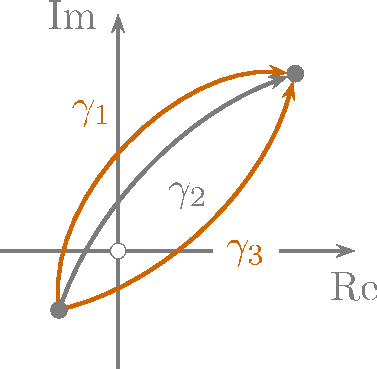
\includegraphics[scale=0.2]{images/ana3-tmp-1}
  \end{figure}
\end{notice}

\begin{theorem}[Definition]
  \begin{enum-arab}
    \item $z = x + \mathrm{i} y \, \implies \, \overline{z} = x - \mathrm{i} y$ heißt \acct{konjugiert komplexe Zahl} zu $z$.

    \item $|z| = \sqrt{x^2 + y^2} = \sqrt{z \cdot \overline{z}}$ heißt \acct{Betrag} von $z$.

    \item Polardarstellung: Sei $z = x + \mathrm{i} y = |z| (\cos \varphi + \mathrm{i} \sin \varphi)$, wobei $\varphi = \arg(z)$ (\acct{Argument} von $z$) eindeutig gegeben ist durch
    %
    \begin{align*}
      - \pi \leq \varphi < \pi \; , \quad \cos \varphi = \frac{x}{\sqrt{x^2 + y^2}} \; , \quad \sin \varphi = \frac{y}{\sqrt{x^2 + y^2}}.
    \end{align*}
    %
    Rechnen mit Polardarstellung:
    %
    \begin{align*}
      z_1 \cdot z_2 &= |z_1| \cdot |z_2| ( \cos(\varphi_1 + \varphi_2) + \mathrm{i} \sin(\varphi_1 + \varphi_2) ) \\
      z^n &= |z|^n (\cos n \varphi + \mathrm{i} \sin n \varphi)
    \end{align*}
    %
    Die Lösung von $z^n = r (\cos \varphi + \mathrm{i} \sin \varphi)$ ist gegeben durch
    %
    \begin{align*}
      |z| &= r^{1/n}, \\
      \varphi &= \frac{\psi}{n} + \frac{2 \pi k}{n} \; , \quad k = 0,1,\ldots,n-1.
    \end{align*}
  \end{enum-arab}
\end{theorem}

\begin{theorem}[Satz]
  $(\mathbb{C},+,\cdot,|\cdot|)$ ist ein \acct{bewerteter Körper}, das heißt für $|\cdot| : \mathbb{C} \to \mathbb{R}$ gelten:
  %
  \begin{enum-arab}
    \item $|z| \geq 0 \; \land \; (|z| = 0 \iff z = 0)$

    \item $|z_1 \cdot z_2| = |z_1| \cdot |z_2|$

    \item $|z_1 + z_2| \leq |z_1| + |z_2|$ ($\bigtriangleup$-Ungleichung)

    Außerdem gilt die >>$\bigtriangleup$-Ungleichung nach unten<<:
    %
    \begin{align*}
      |z_1 \pm z_2| \geq \Big| |z_1| - |z_2| \Big|
    \end{align*}
  \end{enum-arab}
\end{theorem}

\begin{theorem}[Definition]
  Eine Folge $(z_n)$ in $\mathbb{C}$ \acct{konvergiert} gegen $z \in \mathbb{C}$, falls
  %
  \begin{align*}
    \forall \, \varepsilon > 0 \, \exists \, N_\varepsilon \in \mathbb{N} \, \forall \, n > N_\varepsilon : |z_n - z| < \varepsilon.
  \end{align*}
  %
  Man schreibt $z = \lim\limits_{n \to \infty} z_n$ oder $z_n \to z \; (n \to \infty)$.
\end{theorem}

\begin{theorem}[Satz] \label{thm:1.6}
  Es gelte $z_n \to z$ und $w_n \to w$ in $\mathbb{C}$. Dann gelten
  \begin{enum-arab}
    \item $z_n \pm w_n \to z \pm w$,

    $\lim\limits_{n \to \infty} (z_n + w_n) = \lim\limits_{n \to \infty} z_n + \lim\limits_{n \to \infty} w_n$.

    \item $z_n \cdot w_n \to z \cdot w$,

    \item Falls $w \neq 0$ und
    %
    \begin{align*}
      w_n' \coloneq
      \begin{cases}
        1 & \text{falls } w_n = 0 \\
        w_n & \text{sonst}
      \end{cases},
    \end{align*}
    %
    dann
    %
    \begin{align*}
      \frac{z_n}{w_n} \to \frac{z}{w}.
    \end{align*}

    \item $z_n \to z \, \iff \, \Re\, z_n \to \Re\, z \, \land \, \Im\, z_n \to \Im\, z$.
  \end{enum-arab}
\end{theorem}

\begin{theorem}[Definition]
  \begin{enum-arab}
    \item Seien $r > 0$, $z_0 \in \mathbb{C}$. Dann heißt
    %
    \begin{align*}
      K_r(z_0) \coloneq \{ z \in \mathbb{C} : |z - z_0| < r \}
    \end{align*}
    %
    offene Kreisscheibe um $z_0$.

    \begin{figure}[H]
      \centering
      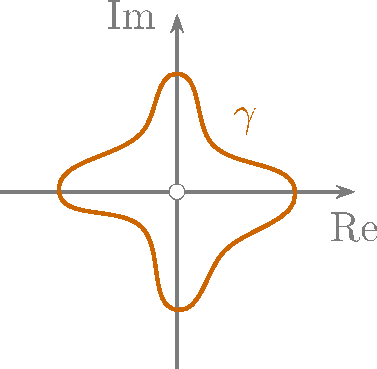
\includegraphics[scale=0.2]{images/ana3-tmp-2}
    \end{figure}

    \item Eine Teilmenge $O \subseteq \mathbb{C}$ heißt \acct{offen}, falls
    %
    \begin{align*}
      \forall \, z \in O \, \exists \, r_z > 0 : K_{r_z}(z) \subseteq O
    \end{align*}
    %
    $A \subseteq \mathbb{C}$ heißt \acct{abgeschlossen}, falls $\mathbb{C} \setminus A$ offen.

    Beliebige Vereinigungen und endliche Schnitte offener Mengen sind offen. Beliebige Schnitte und endliche Vereinigungen abgeschlossener Mengen sind abgeschlossen.

    Für eine beliebige Teilmenge $M \subseteq \mathbb{C}$ ist
    %
    \begin{align*}
      \mathring{M} \coloneq \underset{O \in \{O \subseteq \mathbb{C} : O \, \mathrm{offen} \, \land \, O \subseteq M \}}{\bigcup} O \quad \text{(ist offen)}
    \end{align*}
    %
    das \acct{Innere} von $M$ (die größte offene Menge $O \subseteq M$)
    %
    \begin{align*}
      \overline{M} \coloneq \underset{A \in \{A \subseteq \mathbb{C} : A \, \mathrm{abgeschlossen} \, \land \, M \subseteq A \}}{\bigcap} A \quad \text{(ist abgeschlossen)}
    \end{align*}
    %
    der \acct{Abschluss} von $M$ (die kleinste abgeschlossene Menge $A$ mit $M \subseteq A$)
  \end{enum-arab}
\end{theorem}

\begin{example}
  \begin{enum-arab}
    \item $\emptyset$, $\mathbb{C}$ sind offen und abgeschlossen. Alle anderen Teilmengen von $\mathbb{C}$ sind entweder offen, abgeschlossen oder keins von beidem (beispielsweise halboffene Intervalle).

    \item $K_r(z_0)$ ist offen.
    %
    \begin{align*}
      \overline{K_r(z_0)} = \{ z \in \mathbb{C} : |z-z_0| \leq r \}
    \end{align*}

    \item $\mathbb{R}$ ist nicht offen in $\mathbb{C}$.

	Für $z_0\in \mathbb{R}$ ist für beliebig kleines $r>0$ stets
    %
    \begin{align*}
      K_r(z_0) \;\cap\; \mathbb{C} \setminus \mathbb{R} \neq \emptyset.
    \end{align*}

    \begin{figure}[H]
      \centering
      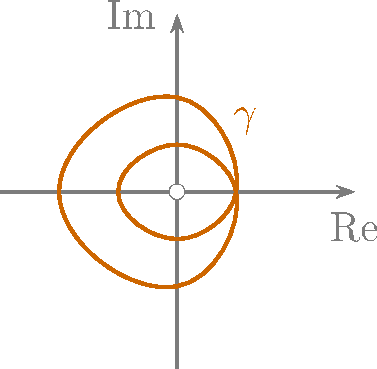
\includegraphics[scale=0.2]{images/ana3-tmp-3}
    \end{figure}

    Ist $\mathbb{R} \subseteq \mathbb{C}$ abgeschlossen? Ja. $\iff$ Ist $\mathbb{C} \setminus \mathbb{R}$ offen? Ja.
  \end{enum-arab}
\end{example}

\begin{theorem}[Definition]
  Sei $O \subseteq \mathbb{C}$ offen, $f : O \to \mathbb{C}$. Dann heißt $f$ \acct{stetig} in $z_0 \in O$, falls
  %
  \begin{align*}
    \forall \, \varepsilon > 0 \, \exists \, \delta_\varepsilon \, \forall \, z \in O : |z - z_0| < \delta \implies |f(z) - f(z_0)| < \varepsilon
  \end{align*}
  %
  oder
  %
  \begin{align*}
    \forall \, (z_n) \text{ Folge in $O$} : z_n \to z_0 \implies f(z_n) \to f(z_0).
  \end{align*}
  %
  $f$ heißt stetig, falls $f$ in jedem $z_0 \in O$ stetig ist.
\end{theorem}

\begin{theorem}[Satz]
  \begin{enum-arab}
    \item Seien $f,g : O \to \mathbb{C}$, $z_0 \in O$, $f,g$ stetig in $z$. Dann sind
    %
    \begin{align*}
      f \pm g \; , \quad f \cdot g \; , \quad \frac{f}{g} \; \text{ falls $g(z_0) \neq 0$}
    \end{align*}
    %
    stetig in $z_0$.

    \item Sei $f : O \to \widetilde{O} \subseteq \mathbb{C}$ stetig in $z_0 \in O$ und $g : \widetilde{O} \to \mathbb{C}$ stetig in $f(z_0)$.

    Dann ist $g \circ f$ stetig in $z_0$. Beweis über Folgen.
  \end{enum-arab}
\end{theorem}

\begin{notice}
  Stetigkeit genauso für $f: M \to \mathbb{C}$ mit beliebiger Menge $M \subseteq \mathbb{C}$.
\end{notice}

\begin{theorem}[Funktionenfolgen]
  Sei $M \subseteq \mathbb{C}$, $f_n$, $f : M \to \mathbb{C}$
  %
  \begin{enum-arab}
    \item $(f_n)$ heißt \acct{punkteweise konvergent} gegen $f$ auf $M$, falls
    %
    \begin{align*}
      \forall \, z \in M \, \forall \, \varepsilon > 0 \, \exists \, N_{\varepsilon,z} \in \mathbb{N} \, \forall \, n > N_{\varepsilon,z} \, : \, |f_n(z) - f(z)| < \varepsilon.
    \end{align*}
    %
    \item $(f_n)$ heißt \acct{gleichmäßig konvergent} gegen $f$ auf $M$, falls
    %
    \begin{align*}
      \forall \, \varepsilon > 0 \, \exists \, N_{\varepsilon} \in \mathbb{N} \, \forall \, n > N_{\varepsilon} \, \forall \, z \in M \, : \, |f_n(z) - f(z)| < \varepsilon.
    \end{align*}
  \end{enum-arab}
\end{theorem}

\begin{theorem}[Satz]
  Seien $f_n : M \to \mathbb{C}$ stetig, $(f_n)$ gleichmäßig konvergent auf $M$ gegen $f$. Dann ist $f$ auch stetig auf $M$.
  %
  \begin{proof}
    Seien $z_0 \in M$, $\varepsilon > 0$ fest und
    %
    \begin{align*}
      |f(z) - f(z_0)| \leq |f(z) - f_n(z)| + |f_n(z) - f_n(z_0)| + |f_n(z_0)-f(z_0)|.
    \end{align*}
    %
    \textbf{1. Schritt:} Wähle ein $N_{\varepsilon}$ so, dass $|f(z) - f_n(z)| < \varepsilon/3$ für $n > N_{\varepsilon}$ und beliebige $z$ (gleichmäßige Konvergenz von $f_n$), also
    %
    \begin{align*}
      |f(z) - f(z_0)| \leq \underbrace{|f(z) - f_n(z)|}_{< \varepsilon/3} + |f_n(z) - f_n(z_0)| + \underbrace{|f_n(z_0)-f(z_0)|}_{< \varepsilon/3}.
    \end{align*}
    %
    \textbf{2. Schritt:} Setze $n \coloneq N_{\varepsilon} + 1$ und nutze die Stetigkeit von $f_n$. Für $|z - z_0| < \delta$ gilt, dann
    %
    \begin{align*}
      |f(z) - f(z_0)| &\leq \underbrace{|f(z) - f_n(z)|}_{< \varepsilon/3} + \overbrace{|f_n(z) - f_n(z_0)|}^{\mathclap{{|f_{N_{\varepsilon} + 1}(z) - f_{N_{\varepsilon} + 1}(z_0)| < \varepsilon/3}}} + \underbrace{|f_n(z_0)-f(z_0)|}_{< \varepsilon/3} \\
      &\leq \frac{\varepsilon}{3} + \frac{\varepsilon}{3} + \frac{\varepsilon}{3} = \varepsilon.
    \end{align*}
    %
  \end{proof}
\end{theorem}

\begin{theorem}[Definition]
  Eine Reihe $\sum\limits_{n=0}^{\infty} a_n$ heißt \acct{absolut konvergent}, falls $\sum\limits_{n=0}^{\infty} |a_n|$ konvergent ist.
\end{theorem}

\begin{theorem}[Weierstraß-Kriterium] \label{thm:1.14}
  Ist $\sum\limits_{n=0}^{\infty} a_n$ mit $a_n \geq 0$ konvergent und gilt $f_n : M \to \mathbb{C}$, $|f_n(z)| \leq a_n$ auf $M \subseteq \mathbb{C}$, so ist die Reihe $\sum\limits_{n=0}^{\infty} f_n(z)$ gleichmäßig konvergent auf $M$ und absolut konvergent für $z \in M$.
\end{theorem}

\begin{example}
  Seien $M \coloneq \overline{K_2(0)} \subseteq \mathbb{C}$, $f_n(z) \coloneq \frac{z^n}{(n+1)^2 2^n}$. Wähle
  %
  \begin{align*}
    a_n \coloneq \frac{1}{(n+1)^2} \; \implies \;
    \begin{dcases}
      \sum\limits_{n=0}^{\infty} \frac{1}{(n+1)^2} < \infty \; , \quad \text{d.h. konvergent} \\
      |f_n(z)| \leq a_n
    \end{dcases}
  \end{align*}
  %
  $\implies$ $g(z) \coloneq \sum\limits_{n=0}^{\infty} f_n(z)$ ist stetig auf $\overline{K_2(0)}$
\end{example}

\begin{theorem}[Potenzreihen]
  Sei $(a_n)$ eine Folge in $\mathbb{C}$,
  %
  \begin{align*}
    R \coloneq \frac{1}{\limsup\limits_{n \to \infty} \sqrt[n]{|a_n|}} \; , \quad \text{mit } \frac{1}{0} \coloneq \infty, \frac{1}{\infty} \coloneq 0.
  \end{align*}
  %
  Dann konvergiert die Potenzreihe
  %
  \begin{align*}
    f(z) \coloneq \sum\limits_{n=0}^{\infty} a_n (z-z_0)^n
  \end{align*}
  %
  für $|z - z_0| < R$ und divergiert für $|z - z_0| > R$. Sie konvergiert gleichmäßig auf jedem Kreis $\overline{K_r(z_0)}$ mit $0 < r < R$. Insbesondere ist $f$ stetig auf $K_R(z_0)$.

  \begin{figure}[H]
    \centering
    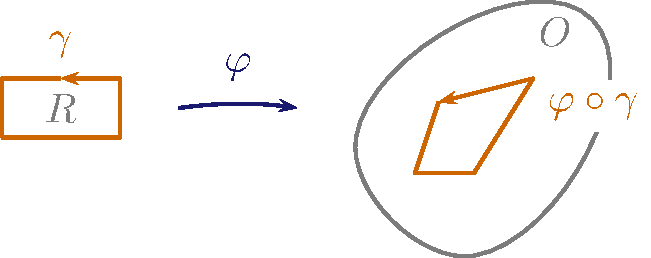
\includegraphics[scale=0.2]{images/ana3-tmp-4}
    \vspace*{-2em}
  \end{figure}
  %
  Falls
  %
  \begin{align*}
    \left| \frac{a_{n+1}}{a_n} \right|
  \end{align*}
  %
  konvergent ist, gilt
  %
  \begin{align*}
    R = \dfrac{1}{\lim_{n\to \infty} \left| \frac{a_{n+1}}{a_n} \right|}.
  \end{align*}
\end{theorem}

\begin{theorem}[Definition]
  \begin{align*}
    \mathrm{e}^z &\coloneq \sum\limits_{n=0}^{\infty} \frac{z^n}{n!} \; , \quad \text{für } z \in \mathbb{C} \\
    \cos z &\coloneq \sum\limits_{n=0}^{\infty} (-1)^n \frac{z^{2n}}{(2n)!} \; , \quad \text{für } z \in \mathbb{C} \\
    \sin z &\coloneq \sum\limits_{n=0}^{\infty} (-1)^n \frac{z^{2n + 1}}{(2n + 1)!} \; , \quad \text{für } z \in \mathbb{C}
  \end{align*}
\end{theorem}

\begin{notice*}
  Exemplarisch für $\mathrm{e}^z$:
  %
  \begin{align*}
    \left| \frac{a_{n+1}}{a_n} \right| = \frac{\frac{1}{(n+1)!}}{\frac{1}{n!}} = \frac{1}{n+1} \to 0
  \end{align*}
  %
  $\implies R = \infty$, die Potenzreihe ist konvergent auf ganz $\mathbb{C}$.
\end{notice*}

\begin{theorem}[Cauchy-Produkt von Reihen]
  Ist $\sum\limits_{n=0}^{\infty} a_n$ absolut konvergent und $\sum\limits_{n=0}^{\infty} b_n$ konvergent in $\mathbb{C}$, so gilt
  %
  \begin{align*}
    \left( \sum\limits_{n=0}^{\infty} a_n \right) \left( \sum\limits_{n=0}^{\infty} b_n \right) =
    \sum\limits_{n=0}^{\infty} \left( \sum\limits_{k=0}^{n} a_k b_{n-k} \right)
  \end{align*}
  %
  \begin{proof}
    Seien
    %
    \begin{align*}
      A \coloneq \sum\limits_{n=0}^{\infty} a_n \; , \quad
      B \coloneq \sum\limits_{n=0}^{\infty} b_n \; , \quad
      B_{\ell} \coloneq \sum\limits_{n=0}^{\ell} b_n
    \end{align*}
    %
    \begin{align*}
      \sum\limits_{n=0}^{N} \sum\limits_{k=0}^{n} a_k b_{n-k} &\overset{m = n - k}{=} \sum\limits_{n=0}^{N} \sum\limits_{m=0}^{N-m} a_n b_m = \sum\limits_{n=0}^{N} a_n \underbrace{\sum\limits_{m=0}^{N-m} b_m}_{B_{N-m} - B + B}
    \end{align*}
    %
    \begin{figure}[H]
      \centering
      \vspace*{-2em}
      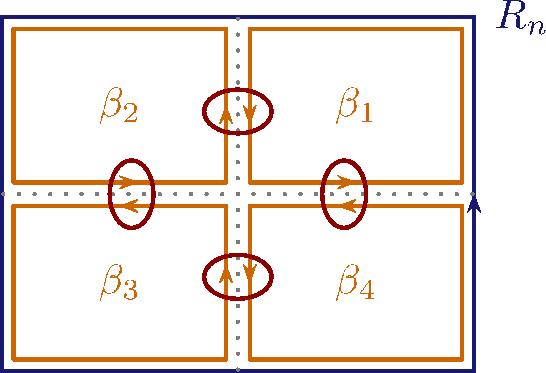
\includegraphics[scale=0.2]{images/ana3-tmp-5}
      \vspace*{-3em}
    \end{figure}
    %
    \begin{align*}
      &\overset{l \coloneq N - n}{\underset{\substack{n = N-\ell}{\ell = 0,1,\ldots,N}}{=}}
        \underbrace{\sum\limits_{\ell = 0}^{N} a_{N - \ell} (B_{\ell} - B)}_{\hypertarget{eq:stern1}{{\color{DarkRed} (\ast)}} \text{ Z.Z. } \to 0} + \underbrace{\sum\limits_{n=0}^{N} a_n B}_{\to A \cdot B} \\
      \hyperlink{eq:stern1}{{\color{DarkRed} (\ast)}} &= \sum\limits_{\ell = 0}^{N_{\varepsilon}} a_{N-\ell} (B_{\ell} - B) + \sum\limits_{\ell=N_{\varepsilon}+1}^{N} a_{N-\ell} (B_{\ell} - B)
    \end{align*}
    %
    \textbf{1. Schritt:} Wähle ein passendes $N_{\varepsilon}$
    %
    \begin{align*}
      \left| \sum\limits_{\ell=N_{\varepsilon}+1}^{N} a_{N-\ell} (B_{\ell} - B) \right|
      &\leq \sup\limits_{\ell \geq N_{\varepsilon}+1} |B_{\ell} - B| \sum\limits_{\ell=N_{\varepsilon}+1}^{N} |a_{N-\ell}| \\
      &\leq \sup\limits_{\ell \geq N_{\varepsilon}+1} |B_{\ell} - B| \sum\limits_{n=0}^{\infty} |a_n| \\
      &\leq \frac{\varepsilon}{2} \; , \quad \text{da } B_{\ell} \to B.
    \end{align*}
    %
    \textbf{2. Schritt:} Abschätzen liefert
    %
    \begin{align*}
      \left| \sum\limits_{\ell = 0}^{N_{\varepsilon}} a_{N-\ell} (B_{\ell} - B) \right|
      &\leq \max\limits_{0 \leq \ell \leq N_{\varepsilon}} |B_{\ell} - B| \sum\limits_{n=N-N_{\varepsilon}}^{\infty} |a_n| \\
      &\leq \frac{\varepsilon}{2} \; , \quad \text{für } N - N_{\varepsilon} > \widetilde{N}_{\varepsilon} \text{ da } \sum\limits_{n=0}^{\infty} |a_n| \text{ konvergent}.
    \end{align*}
    %
    $\implies |\hyperlink{eq:stern1}{{\color{DarkRed} (\ast)}}| < \varepsilon$ für $N - N_{\varepsilon} > \widetilde{N}_{\varepsilon}$ bzw. für $N > \widetilde{N}_{\varepsilon} + N_{\varepsilon}$.
  \end{proof}
\end{theorem}

\begin{notice}[Folgerung]
  \begin{align*}
    \mathrm{e}^{z+w} &= \mathrm{e}^{z} \, \mathrm{e}^{w} \; \, \quad \text{für } z,w \in \mathbb{C}.
  \end{align*}
  %
  \begin{proof} Wir verwenden die Reihendarstellung der Exponentialfunktion.
    \begin{align*}
      \mathrm{e}^{z} \, \mathrm{e}^{w}
      &= \bigg( \sum\limits_{n=0}^{\infty} \underbrace{\frac{z^n}{n!}}_{a_n} \bigg) \bigg( \sum\limits_{n=0}^{\infty} \underbrace{\frac{w^n}{n!}}_{b_n} \bigg)
    \intertext{beide Reihen sind absolut konvergent}
      &= \sum\limits_{n=0}^{\infty} \sum\limits_{k=0}^{n} \frac{z^k}{k!} \frac{w^{n-k}}{(n-k)!} \\
      &= \sum\limits_{n=0}^{\infty} \frac{1}{n!} \sum\limits_{k=0}^{n} \frac{z^k}{k!} \frac{w^{n-k}}{(n-k)!} n! \\
      &= \sum\limits_{n=0}^{\infty} \frac{1}{n!} \sum\limits_{k=0}^{n} \binom{n}{k} z^k w^{n-k} \quad \text{\color{DimGray} Binomischer Lehrsatz} \\
      &= \sum\limits_{n=0}^{\infty} \frac{1}{n!} (z+w)^n = \mathrm{e}^{z+w}
    \end{align*}
  \end{proof}
\end{notice}

\begin{notice}
  Mit der Taylorreihe folgt, dass $\mathrm{e}^z\Big|_{z = x \in \mathbb{R}}$, $\cos z\Big|_{z = x \in \mathbb{R}}$ und $\sin z\Big|_{z = x \in \mathbb{R}}$ dieselben Funktionen sind, wie die aus der Schule bekannten.
\end{notice}

\begin{notice}[Folgerung] \label{thm:1.22}
  \begin{enum-arab}
    \item $\mathrm{e}^{\mathrm{i} z} = \cos z + \mathrm{i} \sin z$ für $z \in \mathbb{C}$ (Eulersche Formel),
    %
    \begin{align*}
      \mathrm{e}^{\mathrm{i} z}
      &= \sum\limits_{n=0}^{\infty} \frac{(\mathrm{i} z)^n}{n!}
      = \sum\limits_{n=0}^{\infty} (-1)^{n} \frac{z^{2n}}{(2n)!} + \mathrm{i} \sum\limits_{n=0}^{\infty} (-1)^{n} \frac{z^{2n+1}}{(2n+1)!}.
    \end{align*}

    \item Mit der Polardarstellung: $z = r (\cos \varphi + \mathrm{i} \sin \varphi)$gilt
    %
    \begin{align*}
      z^n &= r^n \mathrm{e}^{\mathrm{i} n \varphi} \\
      z_1 z_2 &= r_1 r_2 \mathrm{e}^{\mathrm{i} (\varphi_1 + \varphi_2)} \\
      \frac{z_1}{z_2} &= \frac{r_1}{r_2} \mathrm{e}^{\mathrm{i} (\varphi_1 - \varphi_2)}
    \end{align*}
  \end{enum-arab}
\end{notice}

\begin{theorem}[Definition]
  \begin{enum-arab}
    \item $f : O \to \mathbb{C}$ heißt \acct{differenzierbar} in $z_0 \in O$, falls
    %
    \begin{align*}
      f'(z_0) \coloneq \lim\limits_{\substack{z \to z_0}{z \neq z_0}} \frac{f(z) - f(z_0)}{z - z_0}
    \end{align*}
    %
    existiert; $f'(z_0)$ heißt \acct{Ableitung} von $f$ in $z_0$.

    \item $f$ heißt \acct{differenzierbar}, falls $f$ in jedem $z_0 \in \mathbb{C}$ differenzierbar ist. $f' : O \to \mathbb{C}$ heißt \acct{Ableitungsfunktion} von $f$.
  \end{enum-arab}
\end{theorem}

\begin{example} \label{thm:1.23}
  \begin{enum-arab}
    \item Für $f : \mathbb{C} \to \mathbb{C} : z \mapsto c$ ist $f'(z)=0$.

    \item Für $f : \mathbb{C} \to \mathbb{C} : z \mapsto z$ ist $f'(z)=1$.

    \item Für $f : \mathbb{C} \to \mathbb{C} : z \mapsto z^n$ ist $f'(z)=n \, z^{n-1}$.

    \item $f : \mathbb{C} \to \mathbb{C} : z \mapsto |z|^2$ ist in $z_0 \neq 0$ nicht differenzierbar.

    Sei $z_0 = x_0 + \mathrm{i} y_0 \neq 0$:
    %
    \begin{align*}
      z_h &= x_0 + h + \mathrm{i} y_0 \; \implies \; \frac{|z_h|^2 - |z_0|^2}{z_h - z_0} = \frac{2 h x_0 + h^2}{h} \to 2 x_0 \qquad (h \to 0),\\
      z_h &= x_0 + \mathrm{i} (y_0 + h) \; \implies \; \frac{|z_h|^2 - |z_0|^2}{z_h - z_0} = \frac{2 h x_0 + h^2}{\mathrm{i} h} \to - \mathrm{i} 2 x_0 \qquad (h \to 0).
    \end{align*}
  \end{enum-arab}
\end{example}

% % % Vorlesung vom 22.10.2012

\begin{theorem}[Satz]
  Sei $O \subseteq \mathbb{C}$ offen und $f : O \to \mathbb{C}$, $z_0 \in \mathbb{C}$. Dann sind äquivalent:
  %
  \begin{enum-roman}
    \item $f$ ist differenzierbar in $z_0$ mit Ableitung $f'(z_0)$.

    \item $\exists f'(z_0) \in \mathbb{C} : f(z) = f(z_0) + f'(z_0) (z-z_0) + \mathcal{O}(|z-z_0|)$.
  \end{enum-roman}

  \begin{proof}
    \begin{enum-roman}
      \item $\displaystyle \frac{f(z) - f(z_0)}{z-z_0} - f'(z_0) \to 0 \quad \text{für } z \to z_0$.

      \item $\displaystyle \frac{r(z)}{z-z_0} = \frac{f(z) - f(z_0) - (z-z_0) f'(z_0)}{z-z_0} \to 0 \quad \text{für } z \to z_0$.
    \end{enum-roman}
  \end{proof}
\end{theorem}

\begin{theorem}[Satz] \label{thm:1.25}
  \begin{enum-arab}
    \item $f$ differenzierbar in $z_0$ $\implies$ $f$ stetig in $z_0$.

    \item $(f+g)' = f' + g'$.

    \item $(f \, g)' = f' \, g + f \, g'$.

    \item $\displaystyle \left( \frac{f}{g} \right)' = \frac{f' \, g - f \, g'}{g^2} \quad \text{falls } g(z_0) \neq 0$.

    \item $(f \circ g)'(z_0) = f'(g(z_0)) \cdot g'(z_0)$.
  \end{enum-arab}
\end{theorem}

\begin{example}
  \begin{enum-arab}
    \item Polynomfunktionen sind differenzierbar auf $\mathbb{C}$ (folgt aus \ref{thm:1.23}, 3.) und \ref{thm:1.25}, 2.)).

    \item Gebrochen rationale Funktionen sind auf ihrem Definitionsbereich differenzierbar.
  \end{enum-arab}
\end{example}

\begin{theorem}[Definition]
  \begin{enum-arab}
    \item Sei $\gamma \in C^1([a,b] \to \mathbb{C})$ (also auch $\Re \gamma, \Im \gamma \in C^1$). Dann heißt $\gamma$ \acct{Weg} von $z_1 = \gamma(a)$ nach $z_2 = \gamma(b)$. Falls $z_1 = z_2$, heißt $\gamma$ \acct{geschlossen}.

    \item Sei $\gamma$ ein Weg und $f \in C(\mathrm{Bild}(\gamma) \to \mathbb{C})$. Dann heißt
    %
    \begin{align*}
      \int_\gamma f(z) \, \mathrm{d}z &\coloneq \int\limits_{a}^{b} f(\gamma(t)) \, \gamma'(t) \, \mathrm{d}t \\
      &= \int\limits_{a}^{b} \left[ \Re(f(\gamma(t))) \, \Re(\gamma'(t)) - \Im(f(\gamma(t))) \, \Im(\gamma'(t)) \right] \mathrm{d}t \\
      &\phantom{=\;} + \mathrm{i} \int\limits_{a}^{b} \left[ \Im(f(\gamma(t))) \, \Re(\gamma'(t)) + \Re(f(\gamma(t))) \, \Im(\gamma'(t)) \right] \mathrm{d}t
    \end{align*}
    %
    das \acct{Integral von $f$} längs $\gamma$.
  \end{enum-arab}
\end{theorem}

\begin{notice}
  \begin{enum-arab}
    \item Ist $\widetilde{\gamma}$ eine andere Parametrisierung des Weges $\gamma$, sodass folgende Eigenschaften gelten
    %
    \begin{gather*}
      \widetilde{\gamma}(s) = (\gamma \circ \varphi)(s) \quad \text{für } a' \leq s \leq b', \\
      \varphi \in C^1([a',b'] \to [a,b]) \; , \quad \varphi(a') = a \; , \; \varphi(b') = b.
    \end{gather*}
    %
    Dann folgt aus der Substitutionsregel für reelle Integration
    %
    \begin{align*}
      \int_\gamma f(z) \, \mathrm{d}z &= \int\limits_{a}^{b} f(\gamma(t)) \, \gamma'(t) \, \mathrm{d}t \; , \quad \left(t=\varphi(s), \frac {\mathrm{d}t}{\mathrm{d}s} = \varphi'(s)\right) \\
      &= \int\limits_{a'}^{b'} \underbrace{f(\gamma(\varphi(s)))}_{f(\widetilde{\gamma}(s))} \, \underbrace{\gamma'(\varphi(s)) \, \varphi'(s)}_{\frac{\mathrm{d}}{\mathrm{d}s} \widetilde{\gamma}(s) = \frac{\mathrm{d}}{\mathrm{d}s} (\gamma \circ \varphi)(s)} \, \mathrm{d}s \\
      &= \int_{\widetilde{\gamma}} f(z) \, \mathrm{d}z
    \end{align*}

    \item $-\gamma$ ist der zu $\gamma$ entgegengesetzt orientierte Weg.
    %
    \begin{align*}
      -\gamma(t) \coloneq \gamma(a+b-t) \; , \quad a \leq t \leq b.
    \end{align*}
    %
    Es gilt
    %
    \begin{align*}
      \int_{-\gamma} f(z) \, \mathrm{d}z = - \int_{\gamma} f(z) \, \mathrm{d}z.
    \end{align*}

    \item Jede Kurve kann so umparametrisiert werden, dass $a=0$ und $b=1$ gilt.

    \item Verbindungsstrecke: $\gamma = [z_1,z_2]$
    %
    \begin{align*}
      \iff \gamma(t) = z_1 + t(z_2 - z_1) \; , \quad 0 \leq t \leq 1
    \end{align*}

    \begin{figure}[H]
      \centering
      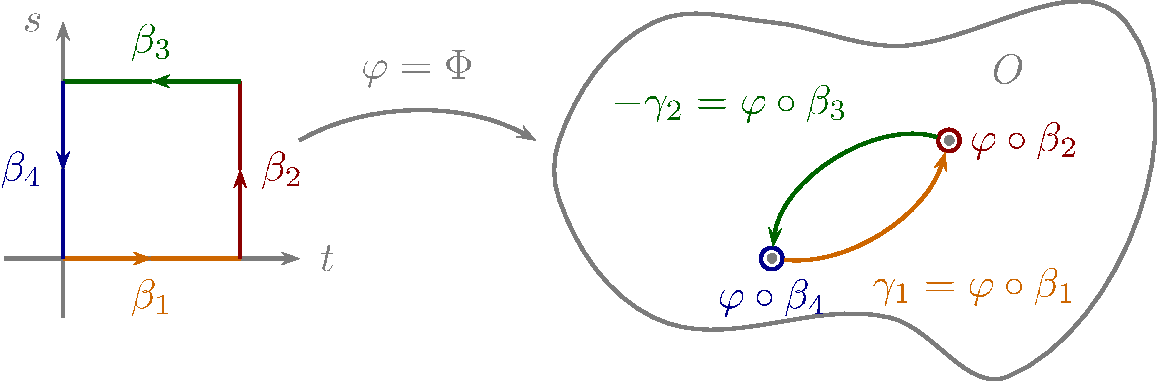
\includegraphics[scale=0.2]{images/ana3-tmp-6}
    \end{figure}

    \item Verallgemeinerung: Ein Weg kann auch nur stückweise $C^1$ sein.
    %
    \begin{align*}
      \gamma \in C([a,b] \to \mathbb{C})
    \end{align*}
    %
    Es existieren $t_0 = a < t_1 < t_2 < \ldots < t_n = b$, sodass
    %
    \begin{align*}
      \gamma_j \coloneq \gamma \Big|_{[t_{j-1},t_j]} \in C^1([t_{j-1},t_j] \to \mathbb{C}).
    \end{align*}
    %
    (das heißt, die Ableitung darf endlich viele Sprünge haben). Dann
    %
    \begin{align*}
      \int_\gamma f(z) \, \mathrm{d}z \coloneq \sum\limits_{j=1}^{n} \int_{\gamma_j} f(z) \, \mathrm{d}z.
    \end{align*}
  \end{enum-arab}
\end{notice}

\begin{example} \label{thm:1.29}
  \begin{enum-arab}
    \item $f(z) \coloneq z^3$, $\gamma = [0,1+\mathrm{i}]$
    %
    \begin{align*}
      \int_{\mathrlap{[0,1+\mathrm{i}]}} z^3 \, \mathrm{d}z
      &= \int\limits_{0}^{1} (t (1+\mathrm{i}))^3 \, (1+\mathrm{i}) \, \mathrm{d}t \\
      &= (1+\mathrm{i})^4 \int\limits_{0}^{1} t^3 \, \mathrm{d}t \\
      &= \frac{(1+\mathrm{i})^4}{4}
    \end{align*}

    \item $f(z) \coloneq \dfrac{1}{z}$, $\gamma(t) = \mathrm{e}^{\mathrm{i} t}$, $0 \leq t \leq 2 \pi$. Da $\gamma(0) = \gamma(2 \pi)$ ist der Weg geschlossen.
    %
    \begin{figure}[H]
      \centering
      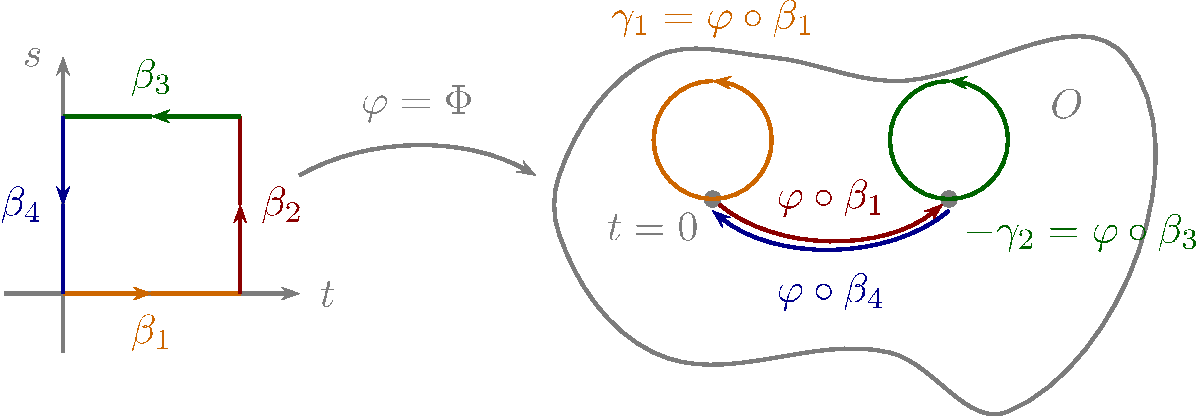
\includegraphics[scale=0.2]{images/ana3-tmp-7}
      \vspace*{-4em}
    \end{figure}
    %
    \begin{align*}
      \int_{\gamma} \frac{1}{z} \mathrm{d}z = \int\limits_{0}^{2 \pi} \frac{1}{\mathrm{e}^{\mathrm{i} t}} \mathrm{i} \mathrm{e}^{\mathrm{i} t} \mathrm{d}t = 2 \pi \mathrm{i} \neq 0
    \end{align*}
  \end{enum-arab}
\end{example}

\begin{theorem}[Satz]
  Sei $O \subseteq \mathbb{C}$ offen, $F : O \to \mathbb{C}$ differenzierbar, $f \coloneq F'$ in $O$ (das heißt, $F$ ist eine \acct{Stammfunktion} von $f$). Ist $\gamma$ ein Weg in $O$, so gilt
  %
  \begin{align*}
    \int_\gamma f(z) \, \mathrm{d}z = F(\gamma(b)) - F(\gamma(a)).
  \end{align*}

  \begin{proof}
    Wegen
    \begin{align*}
      \frac{\mathrm{d}}{\mathrm{d}t} F(\gamma(t)) &= \lim\limits_{\substack{s \to t}{s \neq t}} \frac{F(\gamma(s)) - F(\gamma(t))}{\gamma(s) - \gamma(t)} \, \frac{\gamma(s) - \gamma(t)}{s - t} \\
      &= F'(\gamma(t)) \, \gamma'(t) = f(\gamma(t))  \, \gamma'(t)
    \end{align*}
    %
    können wir die Kettenregel verwenden und es ergibt sich
    %
    \begin{align*}
      \int_\gamma f(z) \, \mathrm{d}z &= \int\limits_{a}^{b} f(\gamma(t)) \, \gamma'(t) \, \mathrm{d}t \\
      &= \int\limits_{a}^{b} \frac{\mathrm{d}}{\mathrm{d}t} F(\gamma(t))  \, \mathrm{d}t \\
      &= \int\limits_{a}^{b} \left[ \frac{\mathrm{d}}{\mathrm{d}t} \Re F(\gamma(t)) + \mathrm{i} \frac{\mathrm{d}}{\mathrm{d}t} \Im F(\gamma(t)) \right] \, \mathrm{d}t.
    \intertext{Nach dem Hauptsatz der Integral- und Differentialrechung im Reellen gilt}
      &= \Big( \Re F(\gamma(b)) + \mathrm{i} \Im F(\gamma(b)) \Big) - \Big( \Re F(\gamma(a)) + \mathrm{i} \Im F(\gamma(a)) \Big) \\
      &= F(\gamma(b)) - F(\gamma(a)).
    \end{align*}
  \end{proof}
\end{theorem}

\begin{notice}[Folgerung]
  \begin{enum-arab}
    \item Besitzt $f$ eine Stammfunktion und ist $\gamma$ geschlossen, so folgt
    %
    \begin{align*}
      \int_\gamma f(z) \, \mathrm{d}z = 0.
    \end{align*}

    \item $f : \mathbb{C} \setminus \{0\} \to \mathbb{C} : z \mapsto \dfrac{1}{z}$ besitzt keine Stammfunktion (siehe \ref{thm:1.29}, 2.)).
  \end{enum-arab}
\end{notice}

\begin{theorem}[Satz] \label{thm:1.32}
  Sei $\gamma$ ein Weg, $f \in C(\mathrm{Bild}(\gamma) \to \mathbb{C})$. Dann
  %
  \begin{align*}
    \left| \int_\gamma f(z) \, \mathrm{d}z \right|
    &\leq \int\limits_{a}^{b} \left| f(\gamma(t)) \right| \, \left| \gamma'(t) \right| \, \mathrm{d}t \\
    &\leq \max\limits_{a \leq t \leq b} \left| f(\gamma(t)) \right| \int\limits_{a}^{b} \left| \gamma'(t) \right| \, \mathrm{d}t.
  \end{align*}

  \begin{proof} Es gilt
    %
    \begin{align*}
      \left| \int_\gamma f(z) \, \mathrm{d}z \right| &= \mathrm{e}^{\mathrm{i} \varphi} \int_\gamma f(z) \, \mathrm{d}z
    \intertext{mit $\varphi = - \arg \left( \int_\gamma f(z) \, \mathrm{d}z \right)$}
      &= \int\limits_{a}^{b} \mathrm{e}^{\mathrm{i} \varphi} \, f(\gamma(t)) \, \gamma'(t) \, \mathrm{d}t \\
      &= \int\limits_{a}^{b} \Re \left( \mathrm{e}^{\mathrm{i} \varphi} \, f(\gamma(t)) \, \gamma'(t) \right) \, \mathrm{d}t
        + \mathrm{i} \int\limits_{a}^{b} \Im \left( \mathrm{e}^{\mathrm{i} \varphi} \, f(\gamma(t)) \, \gamma'(t) \right) \, \mathrm{d}t \\
      &\leq \int\limits_{a}^{b} \left| \Re \left( \mathrm{e}^{\mathrm{i} \varphi} \, f(\gamma(t)) \, \gamma'(t) \right) \right| \, \mathrm{d}t \\
      &\leq \int\limits_{a}^{b} \left| \mathrm{e}^{\mathrm{i} \varphi} \, f(\gamma(t)) \, \gamma'(t) \right| \, \mathrm{d}t \\
      &\leq \int\limits_{a}^{b} \left| \mathrm{e}^{\mathrm{i} \varphi} \right| \, \left| f(\gamma(t)) \right| \, \left| \gamma'(t) \right| \, \mathrm{d}t.
    \end{align*}
    %
    Genau so, falls $\gamma$ nur stückweise $C^1$.
  \end{proof}
\end{theorem}

\begin{theorem}[Definition]
  %
  \begin{align*}
    L(\gamma) \coloneq \int\limits_{a}^{b} \left| \gamma'(t) \right| \, \mathrm{d}t
  \end{align*}
  %
  heißt \acct{Länge} von $\gamma$. Damit wird \ref{thm:1.32} zu
  %
  \begin{align*}
    \left| \text{Integral von $f$ über $\gamma$} \right| \leq \left( \text{Länge von $\gamma$} \right) \, \left( \text{$\max |f|$ auf $\gamma$} \right).
  \end{align*}
\end{theorem}

\begin{example}
  \begin{enum-arab}
    \item $\gamma \coloneq [z_1,z_2]$, $\gamma(t) = z_1 + t(z_2 - z_1)$
    %
    \begin{align*}
      L(\gamma) = \int\limits_{0}^{1} |z_2 - z_1| \, \mathrm{d}t = |z_2 - z_1|
    \end{align*}

    \item $\gamma \coloneq \mathrm{e}^{\mathrm{i} t}$, $0 \leq t \leq 2 \pi$
    %
    \begin{enum-alph}
      \item
      %
      \begin{align*}
        |2 \pi \mathrm{i}| = \left| \int_\gamma \frac{1}{z} \, \mathrm{d}z \right| \leq \max\limits_{\substack{z = \mathrm{e}^{\mathrm{i} t}}{0 \leq t \leq 2 \pi}} \left| \frac{1}{z} \right| \, \int\limits_{0}^{2 \pi} \left| \mathrm{i} \,  \mathrm{e}^{\mathrm{i} t} \right| \, \mathrm{d}t = 2 \pi
      \end{align*}

      \item
      %
      \begin{align*}
        |0| = \left| \int_\gamma z \, \mathrm{d}z \right| \leq \max\limits_{z = \mathrm{e}^{\mathrm{i} t}} |z| \, 2 \pi = 2 \pi
      \end{align*}
    \end{enum-alph}
  \end{enum-arab}
\end{example}

\begin{theorem}[Satz] \label{thm:1.35}
  Sei $(a_n)$ eine Folge in $\mathbb{C}$, $R = \dfrac{1}{\limsup\limits_{n \to \infty} \sqrt[n]{|a_n|}} > 0$.
  Dann ist
  %
  \begin{align*}
    f(z) = \sum\limits_{n=0}^{\infty} a_n \, z^n \; , \quad \text{für } |z| < R
  \end{align*}
  %
  auf dem offenen Konvergenzkreis $\mathring{K}_R(0)$ beliebig oft differenzierbar mit
  %
  \begin{align*}
    f'(z) = \sum\limits_{n=1}^{\infty} a_n \, n \, z^{n-1} \; , \quad
    f''(z) = \sum\limits_{n=2}^{\infty} a_n \, n \, (n-1) \, z^{n-2} \; , \quad \ldots
  \end{align*}

  \begin{proof} Seien
    %
    \begin{align*}
      g(z) \coloneq \sum\limits_{n=1}^{\infty} a_n \, n \, z^{n-1} \; , \quad R' \coloneq \frac{1}{\limsup\limits_{n \to \infty} \sqrt[n]{|a_n \, n|}}
    \end{align*}
    %
    dann gilt
    %
    \begin{enum-arab}
      \item $R' = R$ wegen $\lim\limits_{n \to \infty} \sqrt[n]{n} = 1$. Das heißt: $g$ ist auf demselben $K_R(0)$ definiert wie $f$.

      \item $g = f'$. Seien $w \in K_R(0)$, $z \in K_R(0) \setminus \{w\}$, so folgt
      %
      \begin{gather*}
        \frac{f(z) - f(w)}{z - w} - g(w) = \sum\limits_{n = 1}^{\infty} a_n \underbrace{\left( \frac{z^n - w^n}{z - w} - n \, w^{n-1} \right)}_{{\hypertarget{eq:stern2}{{\color{DarkRed} (\ast)}}}} \\
        \begin{aligned}
          {\hyperlink{eq:stern2}{{\color{DarkRed} (\ast)}}} &= \left| \frac{1}{z - w} \int_{[w,z]} \left( n \, u^{n-1} - n \, w^{n-1} \right) \mathrm{d}u \right| \\
          &\leq \frac{1}{|z-w|} \, L([w,z]) \, n \, |z^{n-1} - w^{n-1}| \\
          \implies &
          \begin{dcases}
            {\hyperlink{eq:stern2}{{\color{DarkRed} (\ast)}}} \to 0 \; , \quad \text{für } z \to w \\
            |a_n(\ldots)| \leq n \, |z|^{n-1} + n \, |w|^{n-1}
          \end{dcases}
        \end{aligned}
      \end{gather*}
      %
      Die Reihe konvergiert also gleichmäßig in $K_r(0)$ für jedes $r < R$. Der Grenzwert von $z \to w$ und die Reihe sind vertauschbar, also
      %
      \begin{align*}
        \frac{f(z) - f(w)}{z - w} - g(w) \to 0.
      \end{align*}
    \end{enum-arab}
  \end{proof}
\end{theorem}

% % % Vorlesung vom 25.10.2012

\begin{example}
  \begin{enum-arab}
    \item
    %
    \begin{align*}
      \mathrm{e}^z &= \sum\limits_{n=0}^{\infty} \frac{z^n}{n!} \; , \quad z \in \mathbb{C} \\
      (\mathrm{e}^z)' &= \sum\limits_{n=1}^{\infty} \frac{n z^{n-1}}{n!} \overset{k = n-1}{=}
        \sum\limits_{k=0}^{\infty} \frac{z^k}{k!}
    \end{align*}

    \item
    %
    \begin{align*}
      (\cos z)'
      &= \left( \sum\limits_{n=0}^{\infty} (-1)^n \frac{z^{2n}}{(2n)!} \right)' \\
      &= - \sum\limits_{n=1}^{\infty} (-1)^{n-1} \frac{z^{2n-1}}{(2n-1)!} \\
      &\overset{k=n-1}{\underset{\substack{n=k+1}{2n = 2k+2}}{=}}
      - \sum\limits_{k=0}^{\infty} (-1)^{k} \frac{z^{2k+1}}{(2k+1)!} \\
      &= - \sin z \; , \quad \text{für } z \in \mathbb{C}
    \end{align*}

    \item Genauso für $(\sin z)' = \cos z$.
  \end{enum-arab}
\end{example}

\begin{theorem}[Definition]
  Sei $O \subseteq \mathbb{C}$ offen, $\gamma_1, \gamma_2 \in C^1([0,1] \to O)$. Dann heißen $\gamma_1$, $\gamma_2$ \acct{$C^1$-homotop} in $O$, falls es eine Abbildung $\Phi \in C^1([0,1] \times [0,1] \to O)$ gibt, sodass
  %
  \begin{align*}
    \Phi(\cdot,0) = \gamma_1 \; , \quad \Phi(\cdot,1) = \gamma_2
  \end{align*}
  %
  und eine der folgenden Bedingungen
  %
  \begin{enum-roman}
    \item $\Phi(0,s) = \gamma_1(0)$, $\Phi(1,s) = \gamma_1(1)$ für $0 \leq s \leq 1$. Insbesondere folgt daraus, dass $\gamma_1(0) = \gamma_2(0)$ und $\gamma_1(1) = \gamma_2(1)$. Die Kurven stimmen also in den Anfangs- und Endpunkten überein.

    \item $\Phi(0,s) = \Phi(1,s)$ für $0 \leq s \leq 1$. $\gamma_1$ und $\gamma_2$ sind also geschlossen, ebenso die Wege $\beta_s \coloneq \Phi(\cdot,s)$.
  \end{enum-roman}
  %
  Wir schreiben $\gamma_1 \sim \gamma_2$ ($\sim$ ist eine Äquivalenzrelation). $\Phi$ heißt Homotopie zwischen $\gamma_1$ und $\gamma_2$. Ein geschlossener Weg $\gamma$ heißt \acct{nullhomotop}, falls $\gamma$ homotop zu einem konstanten Weg ist.
\end{theorem}

\begin{example}
  \begin{enum-arab}
    \item
    \begin{enum-alph}
      \item $O = \mathbb{C}$. Sind $\gamma_1,\gamma_2 \in C^1([0,1] \to \mathbb{C})$ mit $\gamma_1(0) = \gamma_2(0)$ und $\gamma_1(1) = \gamma_2(1)$, dann gilt $\gamma_1 \sim \gamma_2$:
      %
      \begin{align*}
        \Phi(t,s) \coloneq \gamma_1(t) + s \underbrace{(\gamma_2(t) - \gamma_1(t))}_{=0 \text{ für } t=0, t=1}
      \end{align*}
      %
      \begin{figure}[H]
        \centering
        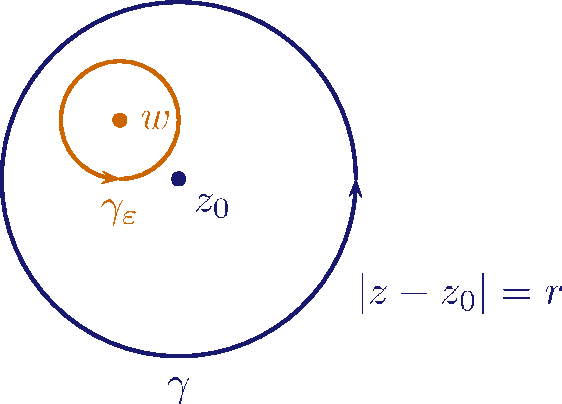
\includegraphics[scale=0.2]{images/ana3-tmp-8}
      \end{figure}

      \item Jeder geschlossene Weg $\gamma \in C^1([0,1] \to \mathbb{C})$ ist in $O \subseteq \mathbb{C}$ nullhomotop: Sei $\gamma_2(t) \coloneq z_0 \in \mathbb{C}$ fest.
      %
      \begin{align*}
        \Phi(t,s) \coloneq \gamma(t) + s (z_0 - \gamma(t))
      \end{align*}
      %
      \begin{figure}[H]
        \centering
        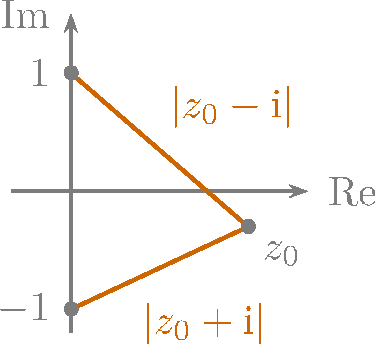
\includegraphics[scale=0.2]{images/ana3-tmp-9}
      \end{figure}
    \end{enum-alph}

    \item $O = \mathbb{C} \setminus \{ 0 \}$
    \begin{enum-alph}
      \item ~
      %
      \begin{figure}[H]
        \centering
        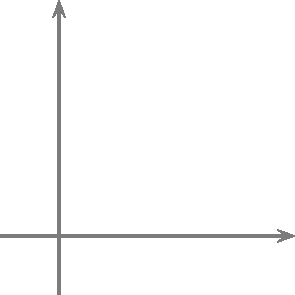
\includegraphics[scale=0.2]{images/ana3-tmp-10}
      \end{figure}
      %
      Offensichtlich: $\gamma_1 \sim \gamma_2$, aber nicht $\gamma_1 \sim \gamma_3$ und auch nicht $\gamma_2 \sim \gamma_3$, weil wir über die $0$ hinüber müssten.

      Anschaulich: Zwei Wege sind homotop, wenn >>dazwischen<< nur Elemente aus $O$ liegen.

      \item ~
      %
      \begin{figure}[H]
        \centering
        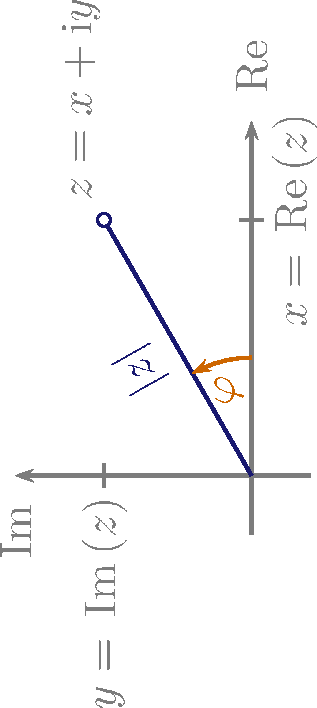
\includegraphics[scale=0.2]{images/ana3-tmp-11}
      \end{figure}
      %
      $\gamma$ ist nicht nullhomotop, aber $\gamma \sim \widetilde{\gamma} : t \mapsto \mathrm{e}^{\mathrm{i} \, 2\pi \, t}$, $0 \leq t \leq 1$

      \item ~
      %
      \begin{figure}[H]
        \centering
        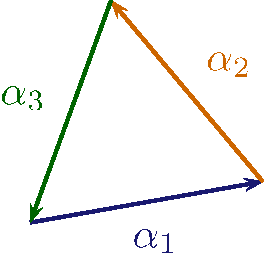
\includegraphics[scale=0.2]{images/ana3-tmp-12}
      \end{figure}

      $\gamma \sim \hat{\gamma} : t \mapsto \mathrm{e}^{\mathrm{i} \, 4\pi \, t}$, $0 \leq t \leq 1$. Zweimal durchlaufener Kreis.
    \end{enum-alph}
  \end{enum-arab}
\end{example}

%
% Henri Menke, 2012 Universität Stuttgart.
%
% Dieses Werk ist unter einer Creative Commons Lizenz vom Typ
% Namensnennung - Nicht-kommerziell - Weitergabe unter gleichen Bedingungen 3.0 Deutschland
% zugänglich. Um eine Kopie dieser Lizenz einzusehen, konsultieren Sie
% http://creativecommons.org/licenses/by-nc-sa/3.0/de/ oder wenden Sie sich
% brieflich an Creative Commons, 444 Castro Street, Suite 900, Mountain View,
% California, 94041, USA.

\section{Holomorphie und Analytizität}
\addtocounter{thmn}{1}
\setcounter{theorem}{0}

% % % Vorlesung vom 25.10.2012

\begin{theorem}[Vereinbarung]
  Zu $f : O \to \mathbb{C}$ setzen wir
  %
  \begin{gather*}
    \widetilde{O} \coloneq \{ (x,y) \in \mathbb{R}^2 : x + \mathrm{i} y \in O \} , \\
    \begin{pmatrix} u \\ v \end{pmatrix} : \widetilde{O} \to \mathbb{R}^2 : (x,y) \mapsto \begin{pmatrix} u(x,y) \\ v(x,y) \end{pmatrix} \coloneq \begin{pmatrix} \Re f(x + \mathrm{i} y) \\ \Im f(x + \mathrm{i} y) \end{pmatrix}.
  \end{gather*}
  %
  $f$ wird interpretiert als Abbildung von $\mathbb{R}^2$ nach $\mathbb{R}^2$.
\end{theorem}

\begin{theorem}[Satz] \label{thm:2.2}
  $O \subseteq \mathbb{C}$ offen, $f : O \to \mathbb{C}$. Dann sind äquivalent:
  %
  \begin{enum-roman}
    \item \label{itm:2.2 i} $f$ ist differenzierbar (in $O$).

    \item \label{itm:2.2 ii} $f$ stetig (in $O$) und für alle Wege $\gamma_1, \gamma_2 \in C^1([0,1] \to O)$ gilt
    %
    \begin{align*}
      \gamma_1 \sim \gamma_2 \implies \int_{\gamma_1} f(z) \, \mathrm{d}z = \int_{\gamma_2} f(z) \, \mathrm{d}z.
    \end{align*}

    \item \label{itm:2.2 iii} $f$ stetig und für alle $\gamma \in C^1([0,1] \to O)$ gilt
    %
    \begin{align*}
      \gamma \text{ nullhomotop } \implies \int_\gamma f(z) \, \mathrm{d}z = 0.
    \end{align*}

    \item \label{itm:2.2 iv} Für jedes $z_0 \in O$ existiert $R > 0$, $(a_n)$ Folge in $\mathbb{C}$, sodass
    %
    \begin{align*}
      f(z) = \sum\limits_{n=0}^{\infty} a_n (z-z_0)^n \; , \quad \text{für } |z-z_0| < R.
    \end{align*}

    \item \label{itm:2.2 v} $f$ ist in $O$ beliebig oft differenzierbar.

    \item \label{itm:2.2 vi} $u, v \in C^1(\widetilde{O} \to \mathbb{R})$ und $u, v$ erfüllen die \acct{Cauchy-Riemannschen Differentialgleichungen}:
    %
    % u_x = \frac{\partial u}{\partial x}
    %
    \begin{align*}
      u_x = v_y \quad \text{und} \quad u_y = -v_x \; , \quad \text{in } \widetilde{O}.
    \end{align*}
  \end{enum-roman}
\end{theorem}

\begin{theorem}[Definition]
  Sei $O \subseteq \mathbb{C}$ offen, $f : O \to \mathbb{C}$. Erfüllt $f$ eine (und damit alle) Bedingungen aus \ref{thm:2.2}, so heißt $f$ \acct{holomorph} (dies betont die beliebige Differenzierbarkeit) oder \acct{analytisch} (dies betont \ref{itm:2.2 iv}).
\end{theorem}

\begin{theorem}[Cauchy'scher Integralsatz für die Bilder von Rechtecken] \label{thm:2.4}
  Sei $O \subseteq \mathbb{C}$ offen, $f : O \to \mathbb{C}$ differenzierbar, $R \coloneq [a,b] \times [c,d]$, $\varphi \in C^1(R \to O)$, $\gamma$ die geschlossene Randkurve von $R$ (stückweise $C^1$). Dann
  %
  \begin{align*}
    \int_{\varphi \circ \gamma} f(z) \, \mathrm{d}z = 0.
  \end{align*}
  %
  \begin{figure}[H]
    \centering
    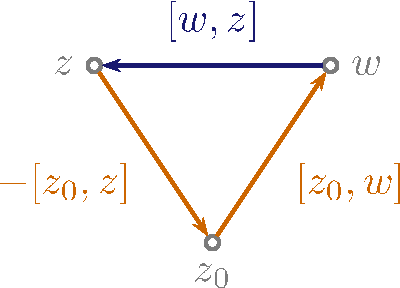
\includegraphics[scale=0.2]{images/ana3-tmp-13}
  \end{figure}
  %
  \begin{proof}
    \begin{enum-arab}
      \item $\varphi \in C^1(R \to O) \implies \varphi \circ \gamma$ ist stückweise $C^1$, also ein Weg in $O$.

      \item Da $R$ kompakt und $\partial_1 \varphi$ und $\partial_2 \varphi$ stetig auf $R$:
      %
      \begin{align*}
        |\nabla \varphi| = \left| \binom{\partial_1 \varphi}{\partial_2 \varphi} \right| \leq c \quad (\leq \infty) \quad  \text{auf } R.
      \end{align*}

      \item \label{itm:2.4 3.} Konstruiere eine Folge $(R_n)$ von Rechtecken mit Randkurven $\gamma_n$:
      %
      \begin{align*}
        R_0 \coloneq R \; , \quad \gamma_0 = \gamma.
      \end{align*}
      %
      Teile $R_n$ durch Seitenhalbierung in vier Rechtecke. Wähle als $R_{n+1}$ dasjenige der vier, für das
      %
      \begin{align*}
        \left| \int_{\varphi \circ \gamma_{n+1}} f(z) \, \mathrm{d}z \right|
      \end{align*}
      %
      am größten ist.
      %
      \begin{figure}[H]
        \centering
        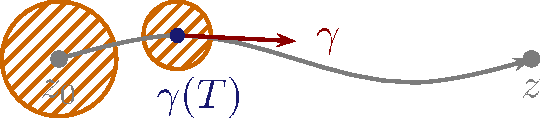
\includegraphics[scale=0.2]{images/ana3-tmp-14}
      \end{figure}
      %
      Integrale über die {\color{DarkRed} rot} markierten Teile heben sich gegenseitig weg.
      %
      \begin{align*}
        \int_{-\gamma} f(z) \, \mathrm{d}z = - \int_{\gamma} f(z) \, \mathrm{d}z.
      \end{align*}
      %
      Daraus folgt
      %
      \begin{align*}
        \int_{\varphi \circ \gamma_n} f(z) \, \mathrm{d}z = \sum\limits_{j = 1}^{4} \int_{\varphi \circ \beta_j} f(z) \, \mathrm{d}z.
      \end{align*}
      %
      Weiterhin folgt
      %
      \begin{align*}
        \left| \int_{\varphi \circ \gamma_n} f(z) \, \mathrm{d}z \right|
        \leq \sum\limits_{j = 1}^{4} \left| \int_{\varphi \circ \gamma_{n+1}} f(z) \, \mathrm{d}z \right|
        \leq 4 \, \left| \int_{\varphi \circ \gamma_{n+1}} f(z) \, \mathrm{d}z \right|.
      \end{align*}
      %
      Durch vollständige Induktion zeigt sich
      %
      \begin{align*}
        \left| \int_{\varphi \circ \gamma_0} f(z) \, \mathrm{d}z \right|
        \leq 4^n \left| \int_{\varphi \circ \gamma_n} f(z) \, \mathrm{d}z \right|.
      \end{align*}

      \item \label{itm:2.4 4.} Sei $x_n$ der Mittelpunkt von $R_n$, dann gilt
      %
      \begin{align*}
        \forall \, x \in R_n : |x - x_n| < L(\gamma_n) \leq \frac{1}{2^n} L(\gamma_0).
      \end{align*}
      %
      Für $m \geq n$ folgt dann
      %
      \begin{align*}
        |x_m - x_n| < \frac{1}{2^n} L(\gamma_0) \; , \quad \text{da } R_m \leq R_n.
      \end{align*}
      %
      Also ist $(x_n)$ Cauchy: $x_m \to y \in R_0$.

      Für $m \geq n$ gilt $x_m \in R_n$, daraus folgt
      %
      \begin{align*}
        |x_n - y| \leq \frac{1}{2^n} L(\gamma_0).
      \end{align*}

      \item \label{itm:2.4 5.} Aus $x_n \to y \in R_0$ folgt mit der Stetigkeit von $\varphi$
      %
      \begin{align*}
        \varphi(x_n) - \varphi(y) \eqcolon z_0 \in O
      \end{align*}
      %
      Sei nun $z = \varphi(x)$ mit $x \in R^n$, dann folgt
      %
      \begin{align*}
        |\Re(z-z_0)| &= |\Re \varphi(x) - \Re \varphi(y)|
      \intertext{und mit dem Mittelwertsatz}
        &= | \nabla (\Re \varphi)(\xi)(x-y)| \\
        &\leq c |x-y| \leq c \, \frac{1}{2^n} L(\gamma_0).
      \end{align*}
      %
      Genauso für $\Im z$
      %
      \begin{align*}
        |z-z_0| \leq \sqrt{2} \, c \, \frac{1}{2^n} L(\gamma_0).
      \end{align*}

% % % Vorlesung vom 29.10.2012

      \item \label{itm:2.4 6.} Sei $\varepsilon > 0$ vorgegeben.
      %
      \begin{align*}
        f(z) = f(z_0) + f'(z_0) (z-z_0) + r(z,z_0)
      \end{align*}
      %
      mit
      \begin{align*}
        \frac{|r(z,z_0)|}{|z-z_0|} < \varepsilon \quad \text{für } |z-z_0| < \delta
      \end{align*}
      %
      Für $n \geq N_\delta$ und gilt
      %
      \begin{align*}
        |z-z_0| < \delta \quad \forall \, z \in \varphi(R_n)
      \end{align*}

      \begin{notice*}
        $\displaystyle |z_n - z_0| < \frac{\delta}{2}$ für $n \geq \widetilde{N}_\delta$

        $\displaystyle |z-z_n| = |\varphi(y)-\varphi(x_n)| \overset{\text{\ref{itm:2.4 5.}}}{\leq} c |y - x_n| \overset{\text{\ref{itm:2.4 4.}}}{<} \frac{\delta}{2}$ für $n > \widetilde{\widetilde{N}}_\delta$
      \end{notice*}

      und somit
      %
      \begin{align*}
        |r(z,z_0)| < \varepsilon |z-z_0| \overset{\text{\ref{itm:2.4 5.}}}{\leq} \sqrt{2} c \frac{\varepsilon}{2^n} L(\gamma_0) \; , \quad z,z_0 \in \varphi(R_n)
      \end{align*}

      \item
      %
      \begin{gather*}
        \begin{aligned}
          \left| \int_{\varphi \circ \gamma_n} f(z) \, \mathrm{d}z \right|
          &\leq \underbrace{\left| \int_{\varphi \circ \gamma_n} \underbrace{\Big(f(z_0) + f'(z_0) (z-z_0)\Big)}_{\text{Besitzt Stammfunktion}} \, \mathrm{d}z \right|}_{=0 \text{ da $\varphi \circ \gamma_n$ geschlossen}}
          + \left| \int_{\varphi \circ \gamma_n} r(z,z_0) \, \mathrm{d}z \right| \\
          &\leq L(\varphi \circ \gamma_n)
          \, \max\limits_{z \in \mathrm{Bild}(\varphi \circ \gamma_n)} |r(z,z_0)| \\
          &\leq \int |(\varphi \circ \gamma_n)'(t)| \mathrm{d}t
          \, \max\limits_{z \in \mathrm{Bild}(\varphi \circ \gamma_n)} |r(z,z_0)| \\
          &\leq \int |\varphi'(\gamma_n(t))| \, |\gamma_n'(t)| \mathrm{d}t
          \, \max\limits_{z \in \mathrm{Bild}(\varphi \circ \gamma_n)} |r(z,z_0)| \\
          &\leq c \cdot L(\gamma_n)
          \, \max\limits_{z \in \mathrm{Bild}(\varphi \circ \gamma_n)} |r(z,z_0)| \\
          &\leq \frac{c}{2^n} L(\gamma_0)
          \, \max\limits_{z \in \mathrm{Bild}(\varphi \circ \gamma_n)} |r(z,z_0)| \\
          &\overset{\text{\ref{itm:2.4 6.}}}{\leq} \frac{c}{2^n} L(\gamma_0) \, \frac{\varepsilon}{2^n} L(\gamma_0) \\
        \end{aligned} \\
        \begin{aligned}
          \overset{\text{\ref{itm:2.4 3.}}}{\implies}& \left| \int_{\varphi \circ \gamma_0} f(z) \, \mathrm{d}z \right|
          \leq 4^n \left| \int_{\varphi \circ \gamma_n} f(z) \, \mathrm{d}z \right| \leq c \, \varepsilon \, L(\gamma_0)^2 \quad \text{für jedes } \varepsilon > 0 \\
          \implies& \int_{\varphi \circ \gamma_n} f(z) \, \mathrm{d}z = 0
        \end{aligned}
      \end{gather*}
    \end{enum-arab}
  \end{proof}
\end{theorem}

\begin{notice}[Folgerung] \label{thm:2.5}
  Sei $O \subseteq \mathbb{C}$ offen, $f : O \to \mathbb{C}$ differenzierbar, $\gamma_1 \sim \gamma_2$ in $O$. Dann
  %
  \begin{align*}
    \int_{\gamma_1} f(z) \, \mathrm{d}z = \int_{\gamma_2} f(z) \, \mathrm{d}z
  \end{align*}

  \begin{proof}
    Sei $\Phi$ die Homotopie, insbesondere
    %
    \begin{gather*}
      \Phi(t,0) = \gamma_1(t) \; , \quad \Phi(t,1) = \gamma_2(t) \\
      \Phi \in C^1([0,1] \times [0,1] \to O)
    \end{gather*}
    %
    Setze zur Anwendung von \ref{thm:2.4} $R \coloneq [0,1] \times [0,1]$, $\varphi \coloneq \Phi$.

    \textbf{Fall 1:} $\Phi(0,1) = \Phi(0,0)$ für $0 \leq s \leq 1$ und $\Phi(1,s) = \Phi(1,0)$

    \begin{figure}[H]
      \centering
      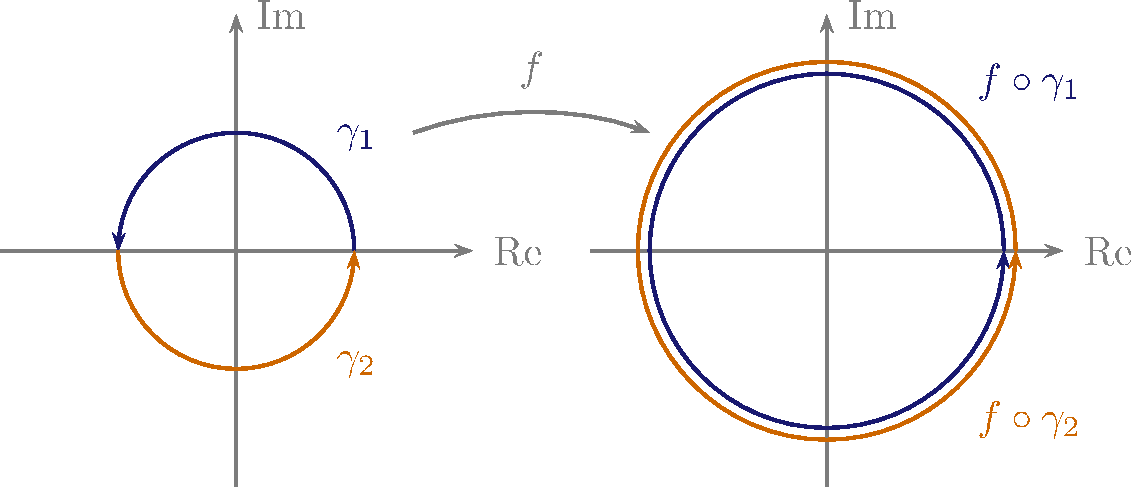
\includegraphics[scale=0.2]{images/ana3-tmp-15}
    \end{figure}

    %
    \begin{gather*}
      \overset{\text{\ref{thm:2.4}}}{\implies}
      \int_{\varphi \circ \beta_1 = \gamma_1} f(z) \, \mathrm{d}z
      + \underbrace{\int_{\varphi \circ \beta_2} f(z) \, \mathrm{d}z}_{=0 \text{, da } \varphi \circ \beta_2 = \mathrm{const.}}
      + \underbrace{\int_{\varphi \circ \beta_3 = -\gamma_2} f(z) \, \mathrm{d}z}_{= - \int_{\gamma_2} f(z) \, \mathrm{d}z}
      + \underbrace{\int_{\varphi \circ \beta_4} f(z) \, \mathrm{d}z}_{=0 \text{, da } \varphi \circ \beta_4 = \mathrm{const.}} = 0 \\
      \implies \int_{\gamma_1} f(z) \, \mathrm{d}z = \int_{\gamma_2} f(z) \, \mathrm{d}z
    \end{gather*}

    \textbf{Fall 2:} $\Phi(0,s) = \Phi(1,s)$ für $0 \leq s \leq t$

    \begin{figure}[H]
      \centering
      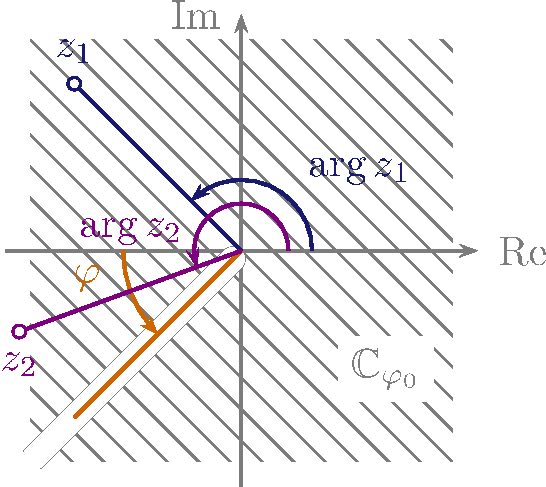
\includegraphics[scale=0.2]{images/ana3-tmp-16}
    \end{figure}

    \begin{gather*}
      \overset{\text{\ref{thm:2.4}}}{\implies}
      \int_{\varphi \circ \beta_1 = \gamma_1} f(z) \, \mathrm{d}z
      + \int_{\varphi \circ \beta_2} f(z) \, \mathrm{d}z
      + \underbrace{\int_{\varphi \circ \beta_3 = - \gamma_2} f(z) \, \mathrm{d}z}_{= - \int_{\gamma_2} f(z) \, \mathrm{d}z}
      + \int_{\varphi \circ \beta_4 = - \varphi \circ \beta_2} f(z) \, \mathrm{d}z = 0 \\
      \implies \int_{\gamma_1} f(z) \, \mathrm{d}z = \int_{\gamma_2} f(z) \, \mathrm{d}z
    \end{gather*}
  \end{proof}
\end{notice}

\begin{proof}[Teilbeweis \ref{thm:2.2}]
  \ref{itm:2.2 i} $\implies$ \ref{itm:2.2 ii}: $f$ differenzierbar $\implies$ $f$ stetig, benutze \ref{thm:2.5}

  \ref{itm:2.2 ii} $\implies$ \ref{itm:2.2 iii}: $\gamma$ nullhomotop $\implies$ $\gamma \sim \widetilde{\gamma}$, da $\widetilde{\gamma} = \text{const.}$, und aus \ref{thm:2.5} folgt
  %
  \begin{align*}
    \int_{\gamma} f(z) \, \mathrm{d}z = \int_{\widetilde{\gamma}} f(z) \, \mathrm{d}z = 0 \; , \quad \text{da } \widetilde{\gamma} = \text{const.} \text{ (Integral über Punkt ist $0$)}
  \end{align*}
\end{proof}

\begin{theorem}[Cauchy-Integralformel für die Kreisscheibe] \label{thm:2.6}
  \text{Kreisscheibe:} Sei $O \subseteq \mathbb{C}$ offen, $f : O \to \mathbb{C}$ differenzierbar, $z_0 \in O$, $r > 0$ mit $\overline{K_r(z_0)} \subseteq O$. Dann gilt
  %
  \begin{align*}
    f(w) = \frac{1}{2 \pi \mathrm{i}} \int_{|z-z_0| = r} \frac{f(z)}{z - w} \, \mathrm{d}z \; , \quad \text{für } |w-z_0| < r
  \end{align*}
  %
  Vereinbarung: Das Integral ist zu verstehen längs der Kurve $\gamma : [0,1] \to O : t \mapsto z_0 + r \, \mathrm{e}^{\mathrm{i} 2 \pi t}$.

  Insbesondere: Ist $f(z)$ auf dem Kreisrand bekannt, dann auch im Kreisinneren.

  \begin{proof} $\gamma_\varepsilon(t) \coloneq w + \varepsilon \, \mathrm{e}^{2 \pi \mathrm{i} t}$, $0 \leq t \leq 1$

    \begin{figure}[H]
      \centering
      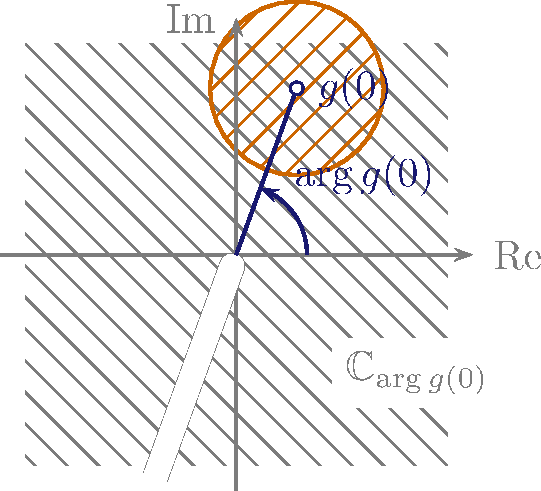
\includegraphics[scale=0.2]{images/ana3-tmp-17}
    \end{figure}

    Offensichtlich: $\gamma \sim \gamma_\varepsilon$ in $O \setminus \{ w \}$ und $f(z)/(z-w)$ ist differenzierbar in $O \setminus \{ w \}$.
    %
    \begin{align*}
      \overset{\text{\ref{thm:2.4}}}{\implies} \int_{|z-z_0| = r} \frac{f(z)}{z-w} \, \mathrm{d}z
      &= \int_{\gamma_\varepsilon} \frac{f(z)}{z-w} \, \mathrm{d}z \\
      &= \underbrace{\int_{\gamma_\varepsilon} \underbrace{\frac{f(z) - f(w)}{z-w}}_{|\cdot| \leq c \text{, weil diffbar}} \, \mathrm{d}z}_{|\cdot| \leq c \, L(\gamma_\varepsilon) = c \, 2 \pi \varepsilon \to 0 \text{ für } \varepsilon \downarrow 0}
      + f(w) \underbrace{\int_{\gamma_\varepsilon} \frac{1}{z-w} \, \mathrm{d}z}_{= 2 \pi \mathrm{i}} \\
      %
      \overset{\varepsilon \downarrow 0}{\implies} \int_{|z-z_0| = r} \frac{f(z)}{z-w} \, \mathrm{d}z &= 2 \pi \mathrm{i} f(w)
    \end{align*}

  \end{proof}
\end{theorem}

\begin{theorem}[Potenzreihenentwicklungssatz] \label{thm:2.7}
  Sei $O \subseteq \mathbb{C}$ offen, $f : O \to \mathbb{C}$ differenzierbar, $z_0 \in O$, $\overline{K_r(z_0)} \subseteq O$. Dann gibt es eine Folge $(a_n) \in \mathbb{C}$ mit
  %
  \begin{align*}
    f(z) = \sum\limits_{n=0}^{\infty} a_n (z-z_0)^n \; , \quad \text{für } |z-z_0| < r
  \end{align*}

  \begin{proof}
    Sei $w \in K_r(z_0)$
    %
    \begin{align*}
      f(w) &\overset{\text{\ref{thm:2.6}}}{=} \frac{1}{2 \pi \mathrm{i}} \int_{|z-z_0| = r} \frac{f(z)}{z-w} \, \mathrm{d}z \\
      &= \frac{1}{2 \pi \mathrm{i}} \int_{|z-z_0| = r} f(z) \frac{1}{z-z_0-(w-z_0)} \, \mathrm{d}z \\
      &= \frac{1}{2 \pi \mathrm{i}} \int_{|z-z_0| = r} f(z) \frac{1}{z-z_0} \frac{1}{1-\frac{w-z_0}{z-z_0}} \, \mathrm{d}z \\
      &= \frac{1}{2 \pi \mathrm{i}} \int_{|z-z_0| = r} f(z) \frac{1}{z-z_0} \sum\limits_{n=0}^{\infty} \left( \frac{w-z_0}{z-z_0} \right)^n \, \mathrm{d}z
    \end{align*}
    %
    \begin{notice*}
      Die geometrische Reihe konvergiert, weil $\left| \frac{w-z_0}{z-z_0} \right| = \frac{|w-z_0|}{r} < 1$.
      %
      \begin{align*}
        &\sum\limits_{n=0}^{\infty} \left(\frac{|w-z_0|}{r}\right)^n \text{ konvergent } \\
        \overset{\text{Weierstraß}}{\underset{\text{\ref{thm:1.14}}}{\implies}}
        &\text{ Reihe gleichmäßig konvergent bezüglich $z$}
      \end{align*}
    \end{notice*}
    %
    Reihe und Integral vertauschen
    %
    \begin{align*}
      = \sum\limits_{n=0}^{\infty} \underbrace{\frac{1}{2 \pi \mathrm{i}} \int_{|z-z_0| = r} \frac{f(z)}{(z-z_0)^{n+1}} \, \mathrm{d}z}_{a_n} \left( w-z_0 \right)^n
    \end{align*}
  \end{proof}
\end{theorem}

\begin{notice}[Folgerung]
  Unter diesen Voraussetzungen gilt für den Konvergenzradius $R$ der Potenzreihe
  %
  \begin{align*}
    R \geq \sup \{ r > 0 : \overline{K_r(z_0)} \subseteq O \}
  \end{align*}
\end{notice}

\begin{example}
  $O = \mathbb{C} \setminus \{ \pm \mathrm{i} \}$, $f(z) = \dfrac{1}{1+z^2}$

  \begin{figure}[H]
    \centering
    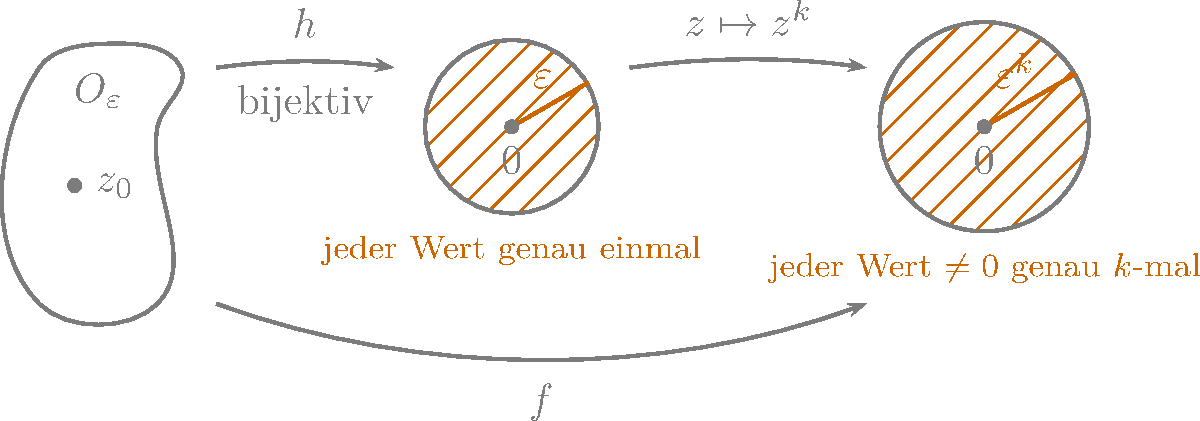
\includegraphics[scale=0.2]{images/ana3-tmp-18}
  \end{figure}

  Entwickle $f$ um $z_0$ in eine Potenzreihe mit Konvergenzradius $R$. Aus 2.8 folgt
  %
  \begin{align*}
    R \geq \min \{ |z_0+\mathrm{i}|,|z_0-\mathrm{i}| \}
  \end{align*}
  %
  Da $|f(z)| \to \infty$ für $z \to \pm \mathrm{i}$ kann die Potenzreihe in $z = \pm \mathrm{i}$ nicht konvergieren.
  %
  \begin{align*}
    \implies R = \min \{ |z_0+\mathrm{i}|,|z_0-\mathrm{i}| \}
  \end{align*}
\end{example}

% % % Vorlesung vom 5.11.2012

\begin{notice}[Folgerung] \label{thm:2.10}
  \begin{enum-arab}
    \item
    \begin{align*}
      a_n = \frac{1}{2 \pi \mathrm{i}} \int_{|z-z_0| = r} \frac{f(z)}{(z-z_0)^{n+1}} \, \mathrm{d}z \text{ für die $a_n$ in \ref{thm:2.7}}
    \end{align*}

    \item
    \begin{align*}
      f(z) &= \sum\limits_{n=0}^{\infty} a_n (z-z_0)^n \overset{\text{Übung}}{\implies} a_n = \frac{f^{(n)}(z_0)}{n!} \\
      \implies f^{(n)}(z_0) &= \frac{n!}{2 \pi \mathrm{i}} \int_{|z-z_0| = r} \frac{f(z)}{(z-z_0)^{n+1}} \, \mathrm{d}z
    \end{align*}
    %
    Auf einer Kreisscheibe um $z_0$ gilt analog zur gewöhnlichen Cauchy-Integralformel (\ref{thm:2.6}) sogar allgemeiner:
    %
    \begin{align*}
      f^{(n)}(w) &= \frac{n!}{2 \pi \mathrm{i}} \int_{|z-z_0| = r} \frac{f(z)}{(z-w)^{n+1}} \, \mathrm{d}z \qquad |w-z_0|<r
    \end{align*}
    %
    (Verwende dazu $z_0 := w$ und $r := |w-z_0|$, sowie die Weghomotopie beider Kurven auf der Kreisscheibe)
    Man nennt diese Form auch \acct{Erweiterte Cauchy'sche Integralformel}.
  \end{enum-arab}
\end{notice}

\begin{theorem}[Definition] \label{thm:2.11}
  Ist $f:\mathbb{C} \to \mathbb{C}$ differenzierbar, so heißt $f$ \acct{ganze Funktion}. Dann gilt mit beliebigem $z_0 \in \mathbb{C}$
  %
  \begin{align*}
    f(z) = \sum\limits_{n=0}^{\infty} a_n (z-z_0)^n
  \end{align*}
  %
  mit Konvergenzradius $R = \infty$, $a_n$ gegeben durch \ref{thm:2.10}
\end{theorem}

\begin{example}
  $\mathrm{e}^{(\cdot)}$, Polynomfunktionen, $\sin$, $\cos$ sind ganz.
\end{example}

\begin{proof}[Teilbeweis \ref{thm:2.2}]
  \ref{itm:2.2 i} $\implies$ \ref{itm:2.2 iv}
  %
  \begin{align*}
    & z_0 \in O \; , \quad O \text{ offen} \\
    \implies& \exists \, r > 0 : K_r(z_0) \subseteq O \\
    \implies& \overline{K_{r/2}(z_0)} \subseteq K_r(z_0) \subseteq O \\
    \overset{\text{\ref{thm:2.7}}}{\implies}& \text{\ref{itm:2.2 iv}} \text{ mit } R \geq \frac{r}{2}
  \end{align*}

  \ref{itm:2.2 iv} $\implies$ \ref{itm:2.2 v}: \ref{thm:1.35}

  \ref{itm:2.2 v} $\implies$ \ref{itm:2.2 i}: offensichtlich
\end{proof}

\begin{theorem}[Cauchy-Abschätzung für Taylor-Koeffizienten] \label{thm:2.13}
  Sei $O \subseteq \mathbb{C}$ offen, $f:O \to \mathbb{C}$ differenzierbar, $\overline{K_r(z_0)} \subseteq O$, $|f(z)| \leq M$ auf $|z-z_0| = r$ und
  %
  \begin{align*}
    f(z) = \sum\limits_{n=0}^{\infty} a_n (z-z_0)^n \; , \quad \text{für } |z-z_0| < r
  \end{align*}
  %
  Dann
  %
  \begin{align*}
    \left| \frac{f^{(n)}(z_0)}{n!} \right| = |a_n| \leq \frac{M}{r^n} \; , \quad \text{für } n \in \mathbb{N}
  \end{align*}

  \begin{proof}
    \begin{align*}
      |a_n| &\overset{\text{\ref{thm:2.10}}}{=} \Bigg| \frac{1}{2 \pi \mathrm{i}} \int_{|z-z_0| = r} \underbrace{\frac{f(z)}{(z-z_0)^{n+1}}}_{|\cdot| \leq \frac{M}{r^{n+1}}} \, \mathrm{d}z \Bigg| \\
      &\overset{\text{\ref{thm:1.32}}}{\leq} \frac{1}{2 \pi} \frac{M}{r^{n+1}} \underbrace{L(|z-z_0| = r)}_{2 \pi r} \\
      &= \frac{M}{r^n}
    \end{align*}
  \end{proof}
\end{theorem}

\begin{theorem}[Satz von Liouville]
  Jede ganze Funktion, die beschränkt ist, ist konstant.

  \begin{proof}
    Aus \ref{thm:2.11}
    %
    \begin{align*}
      f(z) = \sum\limits_{n=0}^{\infty} a_n z^n \; , \quad \text{für } z \in \mathbb{C}
    \end{align*}
    %
    Aus \ref{thm:2.13}
    %
    \begin{align*}
      |a_n| \leq \frac{M}{r^n} \text{ wobei } |f(z)| \leq M \; , \quad \overline{K_r(0)} \subseteq \mathbb{C}
    \end{align*}
    %
    Dann folgt mit $r \to \infty$
    %
    \begin{gather*}
      \implies a_n = 0 \; , \quad \text{für } n = 1, 2, \ldots \\
      \implies f(z) = a_0 + 0  \; , \quad \text{für } z \in \mathbb{C}
    \end{gather*}
  \end{proof}
\end{theorem}

\begin{theorem}[Riemannscher Hebbarkeitssatz]
  Sei $O \subseteq \mathbb{C}$ offen, $z_0 \in O$, $f:O \setminus \{ z_0 \} \to \mathbb{C}$ differenzierbar, und
  %
  \begin{align*}
    \exists \, r > 0 \, \exists \, M > 0 : |f(z)| \leq M \; , \quad \text{für } 0 < |z-z_0| < r
  \end{align*}
  %
  Dann kann $f$ in $z=z_0$ holomorph ergänzt werden, d.h. es existiert $a \in \mathbb{C}$, so dass
  %
  \begin{align*}
    \widetilde{f} : O \to \mathbb{C} : z \mapsto
    \begin{cases}
      a & z=z_0 \\
      f(z) & \text{sonst}
    \end{cases}
  \end{align*}
  %
  differenzierbar ist.

  \begin{proof}
    Setze
    %
    \begin{align*}
      g(z) \coloneq
      \begin{cases}
        0 & z=z_0 \\
        (z-z_0)^2 \, f(z) & \text{sonst}
      \end{cases}
    \end{align*}
    %
    Dann ist $g$ in $O \setminus \{ z_0 \}$ differenzierbar und auch in $z_0$
    %
    \begin{align*}
      & \lim\limits_{\substack{z \to z_0}{z \neq z_0}} \frac{g(z) - g(z_0)}{z - z_0} \\
      =& \lim\limits_{\substack{z \to z_0}{z \neq z_0}} \underbrace{(z-z_0)}_{\to 0} \, \overbrace{f(z)}^{\mathclap{\text{beschränkt}}} = 0
    \end{align*}
    %
    \begin{notice*}
      Beschränkte Folge mal Nullfolge ergibt Nullfolge
    \end{notice*}
    %
    \begin{align*}
      \implies & g \text{ differenzierbar in } O \; , \quad g(z_0) = g'(z_0) = 0 \\
      \overset{\text{\ref{thm:2.2}, \ref{itm:2.2 i} $\implies$ \ref{itm:2.2 iv}}}{\implies} &
        g(z) = \sum\limits_{n=0}^{\infty} a_n (z-z_0)^n \; , \quad |z-z_0| \leq r
    \intertext{weil $a_0 = g(z_0) = 0$ und $a_1 = g'(z_0) = 0$, folgt}
     \implies & g(z) = \sum\limits_{n=2}^{\infty} a_n (z-z_0)^n \; , \quad |z-z_0| < r \\
     \implies & f(z) = \frac{g(z)}{(z-z_0)^2} = \sum\limits_{n=2}^{\infty} a_n (z-z_0)^{n-2} \; , \quad \text{für } 0 < |z-z_0| < r
    \end{align*}
    %
    Setze $a \coloneq a_2$ für Definition von $\widetilde{f}$
    %
    \begin{align*}
      \implies & \widetilde{f}(z) = \sum\limits_{n=2}^{\infty} a_n (z-z_0)^{n-2} \; , \quad |z-z_0| < r
    \end{align*}
    %
    also differenzierbar in $O$.
  \end{proof}
\end{theorem}

\begin{example}
  $f : O \to \mathbb{C}$ differenzierbar, $z_0 \in O$
  %
  \begin{align*}
    g(z) \coloneq
    \begin{dcases}
      \frac{f(z) - f(z_0)}{z - z_0} & \text{sonst} \\
      f'(z_0) & z = z_0
    \end{dcases}
  \end{align*}
  %
  Somit ist $g$ holomorph auf $O$.
\end{example}

\begin{theorem}[Hilfssatz]\label{thm:2.17}
  Sei $O \subseteq \mathbb{C}$ offen, $f:O \to \mathbb{C}$ erfülle \ref{itm:2.2 iii} aus \ref{thm:2.2}. Dann: Ist $D \subseteq O$ eine abgeschlossene Dreiecksfläche mit geschlossener Randkurve $\partial D$ (stückweise Intervalle), so gilt
  %
  \begin{align*}
    \int_{\partial D} f(z) \, \mathrm{d}z = 0
  \end{align*}

  \begin{proof}
    Hauptidee: $\partial D$ umparametrisieren zu einer $C^1$-Kurve
    %
    \begin{align*}
      p(t) \coloneq 3 t^2 - 2 t^3
    \end{align*}

    \begin{figure}[H]
      \centering
      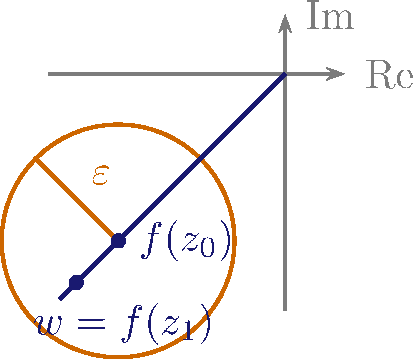
\includegraphics[scale=0.2]{images/ana3-tmp-19}
    \end{figure}

    \begin{align*}
      \implies
      \begin{dcases}
        p(0) = 0 \; , \quad p(1) = 1 \\
        p'(t) > 0 \; , \quad \text{für } 0 < t < 1 \\
        p'(0) = 0 \; , \quad p'(1) = 0
      \end{dcases}
    \end{align*}
    %
    Sei $\partial D : [0,3] \to O$ gegeben durch
    %
    \begin{align*}
      \gamma(t) =
      \begin{dcases}
        \alpha_1(t) & 0 \leq t \leq 1 \\
        \alpha_2(t) & 1 \leq t \leq 2 \\
        \alpha_3(t) & 2 \leq t \leq 3
      \end{dcases}
    \end{align*}

    \begin{figure}[H]
      \centering
      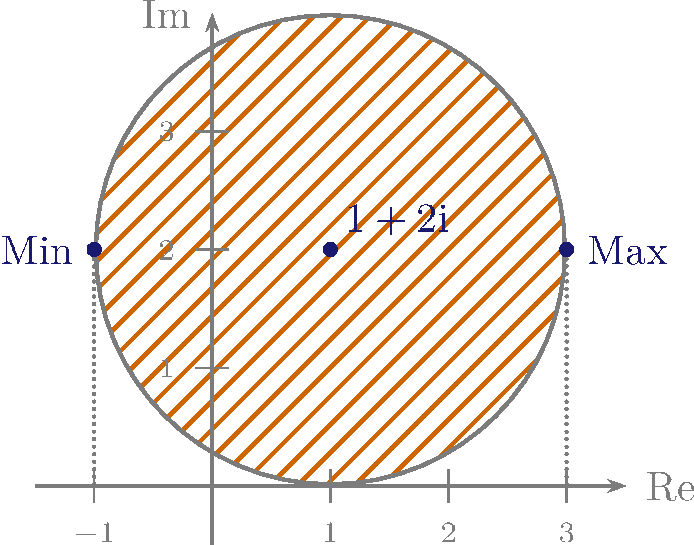
\includegraphics[scale=0.2]{images/ana3-tmp-20}
    \end{figure}

    Sei $\beta_1(t) \coloneq \alpha_1(p(3t))$, $0 \leq t \leq 1/3$
    %
    \begin{align*}
      \implies \int_{\beta_1} f(z) \, \mathrm{d}z \overset{\text{1.28}}{=} \int_{\alpha_1} f(z) \, \mathrm{d}z \; , \quad \beta_1'(0) = 0 , \; \beta_1'\left(\frac{1}{3}\right) = 0
    \end{align*}
    %
    Genauso
    %
    \begin{align*}
      \beta_2(t) &\coloneq \alpha_2\left( 1 + p \left( 3 \left( t - \frac{1}{3} \right) \right) \right) \; , \quad \frac{1}{3} \leq t \leq \frac{2}{3} , \; \beta_2'\left(\frac{1}{3}\right) = 0 , \; \beta_2'\left(\frac{2}{3}\right) = 0 \\
      \beta_3(t) &\coloneq \alpha_3\left( 2 + p \left( 3 \left( t - \frac{2}{3} \right) \right) \right) \; , \quad \frac{2}{3} \leq t \leq 1
    \end{align*}
    %
    Setze
    %
    \begin{gather*}
      \widetilde{\gamma}(t) \coloneq
      \begin{dcases}
        \beta_1(t) & 0 \leq t \leq \frac{1}{3} \\
        \beta_2(t) & \frac{1}{3} \leq t \leq \frac{2}{3} \\
        \beta_3(t) & \frac{2}{3} \leq t \leq 1
      \end{dcases} \\
      \implies \widetilde{\gamma} \in C^1([0,1] \to \mathbb{C}) \text{ ist Randkurve von $D$}
    \end{gather*}
    %
    Dann ist $\widetilde{\gamma}$ nullhomotop:
    %
    \begin{gather*}
      \Phi(t,s) \coloneq \underbrace{(1-s) \widetilde{\gamma}(t) + s \widetilde{\gamma}(0)}_{\in D \subseteq O \text{ da $D$ konvex}} \; , \quad \Phi \in C^1 \\
      \implies \widetilde{\gamma} \sim \widetilde{\gamma}(0) \text{, also $C^1$-nullhomotop} \\
      \overset{\text{\ref{itm:2.2 iii} von \ref{thm:2.2}}}{\implies} \int_{\widetilde{\gamma}} f(z) \, \mathrm{d}z = 0
    \end{gather*}
  \end{proof}
\end{theorem}

\begin{theorem}[Satz von Morera]
  Sei $O \subseteq \mathbb{C}$ offen, $f:O \to \mathbb{C}$ stetig und für jede abgeschlossene Dreiecksfläche $D \subseteq O$ gelte
  %
  \begin{align*}
    \int_{\partial D} f(z) \, \mathrm{d}z = 0
  \end{align*}
  %
  Dann ist $f$ holomorph auf $O$.

  \begin{proof}
    Idee: Zeige, dass $f$ in einem Kreis $K_r(z_0)$ mit $\overline{K_r(z_0)} \subseteq O$ eine Stammfunktion $F$ besitzt. Wähle $z_0 \in O$ und $K_r(z_0)$.

    Setze
    %
    \begin{align*}
      F(z) \coloneq \int_{[z_0,z]} f(\zeta) \, \mathrm{d}\zeta \; , \quad \text{für } z \in K_r(z_0)
    \end{align*}
    %
    Behauptung: $F' = f$ in $K_r(z_0)$. Sei $z \in K_r(z_0)$.
    %
    \begin{align*}
       & \left| \frac{F(w) - F(z)}{w - z} - f(z) \right| \\
      =& \left| \frac{1}{w - z} \left( \int_{[z_0,w]} f(\zeta) \, \mathrm{d}\zeta - \int_{[z_0,z]} f(\zeta) \, \mathrm{d}\zeta - \int_{[z,w]} f(z) \, \mathrm{d}\zeta \right. \right. \\
        & \left. \left. \phantom{\frac{1}{w - z} \qquad} + \int_{[w,z]} f(\zeta) \, \mathrm{d}\zeta + \int_{[z,w]} f(\zeta) \, \mathrm{d}\zeta \right) \right|
    \end{align*}

    \begin{figure}[H]
      \centering
      \caption{Es gilt anschaulich $\int_{[z_0,w]} f(\zeta) \, \mathrm{d}\zeta - \int_{[z_0,z]} f(\zeta) \, \mathrm{d}\zeta + \int_{[w,z]} f(\zeta) \, \mathrm{d}\zeta = 0$}
      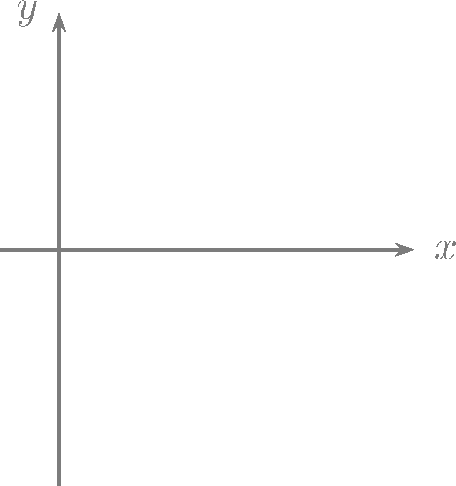
\includegraphics[scale=0.2]{images/ana3-tmp-21}
    \end{figure}

    \begin{align*}
      &= \frac{1}{|w - z|} \left| \int_{[z,w]} \Big( f(\zeta) - f(z) \Big) \, \mathrm{d}\zeta \right| \\
      &\leq \frac{1}{|w - z|} \underbrace{\max\limits_{\zeta \in [z,w]} \Big|f(\zeta) - f(z)\Big|}_{< \varepsilon \text{ für } |w-z| < \delta \text{, da $f$ stetig}} \, \underbrace{L([z,w])}_{=|w-z|} \\
      &< \varepsilon \; , \quad \text{für } |w-z| < \delta
    \end{align*}
    %
    Damit gilt $F' = f$.
    $F$ ist demnach differenzierbar auf $K_r(z_0)$, also nach \ref{thm:2.2} beliebig oft differenzierbar.
    Also ist auch $f$ (beliebig oft) differenzierbar auf $K_r(z_0)$.
    Da $z_0\in O$ beliebig gewählt war, ist $f$ auf ganz $O$ differenzierbar und damit holomorph.
  \end{proof}
\end{theorem}

% % % Vorlesung vom 8.11.2012

\begin{proof}[Teilbeweis \ref{thm:2.2}]
  \ref{itm:2.2 iii} $\overset{\text{\ref{thm:2.17}}}{\implies}$ Vorraussetzung von Morera erfüllt.

  $\overset{\text{Morera}}{\implies}$ \ref{itm:2.2 i} $f$ differenzierbar in $O$.
\end{proof}

\begin{notice}
  \begin{enum-arab}
    \item Beweis von Morera zeigt
    %
    \begin{align*}
      \text{$f$ differenzierbar } &\iff \text{ $f$ besitzt eine lokale Stammfunktion} \\
      &\phantom{\iff} \forall \, z_0 \in O \, \exists \, r > 0 \, \exists \, F : F' = f \text{ in } K_r(z_0)
    \end{align*}

    \item Wenn $f$ differenzierbar in $O$ ist, muss $f$ nicht unbedingt eine globale Stammfunktion (Stammfunktion auf $O$) besitzen: Z.B. $O = K_1(0) \setminus \{0\}$, $f(z) = 1/z$.

    Später: Stammfunktionen können holomorph fortgesetzt werden. Z.B. $\ln z$ als Stammfunktion von $1/z$.
  \end{enum-arab}
\end{notice}

\begin{theorem}[Satz] \label{thm:2.20}
  Sei $O \subseteq \mathbb{C}$ offen, $f : O \to \mathbb{C}$, $z_0 = x_0 + \mathrm{i} y_0 \in O$
  %
  \begin{align*}
    \widetilde{O} &\coloneq \{(x,y) \in \mathbb{R}^2 : x + \mathrm{i} y \in O\} \\
    u(x,y) &\coloneq \Re f(x + \mathrm{i} y) \\
    v(x,y) &\coloneq \Im f(x + \mathrm{i} y)
  \end{align*}
  %
  Es sind äquivalent
  %
  \begin{enum-roman}
    \item \label{itm:2.20 i} $f$ ist differenzierbar in $z_0$.

    \item \label{itm:2.20 ii} $\begin{pmatrix} u \\ v \end{pmatrix} : \widetilde{O} \subseteq \mathbb{R}^2 \to \mathbb{R}^2$ ist differnzierbar in $(x_0,y_0)$ und es gelten die Cauchy-Riemannschen Differentialgleichungen:
    %
    \begin{align*}
      u_x(x_0,y_0) &= v_y(x_0,y_0) \\
      u_y(x_0,y_0) &= -v_x(x_0,y_0) .
    \end{align*}
  \end{enum-roman}
  %
  Sind die Bedingungen erfüllt, so gilt
  %
  \begin{align*}
    u_x(x_0,y_0) &= \Re f'(z_0) \\
    u_y(x_0,y_0) &= - \Im f'(z_0).
  \end{align*}

  \begin{proof}
    %
    \begin{align*}
      &\iff f(z) = f(z_0) + f'(z_0)(z-z_0) + o(|z-z_0|) \\
      &\iff
      \begin{dcases}
        \Re f(z) = \Re f(z_0) + \Re f'(z_0) \Re (z-z_0) - \Im f'(z_0) \Im (z-z_0) \\ \mspace{100mu} + o(|z-z_0|) \\
        \Im f(z) = \Im f(z_0) + \Im f'(z_0) \Re (z-z_0) - \Re f'(z_0) \Im (z-z_0) \\ \mspace{100mu} + o(|z-z_0|)
      \end{dcases}
    \end{align*}
    %
    Sei $z = x + \mathrm{i} y$, dann zerfallen
    %
    \begin{align*}
      \Re (z-z_0) &= x - x_0 \\
      \Im (z-z_0) &= y - y_0
    \end{align*}
    %
    \begin{align*}
      \phantom{\text{\ref{itm:2.20 i}}} &\iff
      \begin{pmatrix}
        u(x,y) \\ v(x,y)
      \end{pmatrix}
      =
      \begin{pmatrix}
        u \\ v
      \end{pmatrix}
      (x_0,y_0) +
      \begin{pmatrix}
        \Re f'(z_0) & -\Im f'(z_0) \\
        \Im f'(z_0) & \Re f'(z_0)
      \end{pmatrix}
      \begin{pmatrix}
        x-x_0 \\
        y-y_0
      \end{pmatrix}\\
      &\phantom{\iff\quad}
      +
      o
      \left(\left|
      \begin{pmatrix}
        x \\ y
      \end{pmatrix}
      -
      \begin{pmatrix}
        x_0 \\ y_0
      \end{pmatrix}
      \right|\right) \\
      %
      &\iff
      \begin{pmatrix}
        u \\ v
      \end{pmatrix}
      \text{ ist differenzierbar in } (x_0,y_0) \text{ mit der Jacobi-Matrix} \\
      &\phantom{\iff\quad}
      \begin{pmatrix}
        \Re f'(z_0) & -\Im f'(z_0) \\
        \Im f'(z_0) & \Re f'(z_0)
      \end{pmatrix}
      =
      \begin{pmatrix}
        u_x & u_y \\
        v_x & v_y
      \end{pmatrix}
      (x_0,y_0)
    \end{align*}
  \end{proof}
\end{theorem}

\begin{proof}[Restbeweis \ref{thm:2.2}]
  \ref{itm:2.2 vi} $\implies$ $\begin{pmatrix} u \\ v \end{pmatrix} : \widetilde{O} \to \mathbb{R}^2$ differenzierbar und es gelten die Cauchy-Riemannschen Differentialgleichungen. $\overset{\text{\ref{thm:2.20}}}{\implies}$ \ref{itm:2.2 i}

  \ref{itm:2.2 i} $\overset{\text{\ref{thm:2.20}}}{\implies}$ $\begin{pmatrix} u \\ v \end{pmatrix}$ differenzierbar in $O$ und es gelten die Cauchy-Riemannschen Differentialgleichungen.

  $\implies$ \ref{itm:2.2 v} $\implies$ $f'$ stetig $\overset{\text{\ref{thm:2.20}}}{\implies}$ $u_x$, $u_y$, $v_x$, $v_y$ stetig

  $\implies$ \ref{itm:2.2 vi}
\end{proof}

\begin{example}
  Sei $O = \mathbb{C}$, $f(z) = \sin z = \frac{1}{2 \mathrm{i}} \left( e^{\mathrm{i} z} - e^{-\mathrm{i} z} \right)$. Zum selbst nachrechnen
  %
  \begin{align*}
    = \underbrace{\cosh y \sin x}_{u(x,y)} + \mathrm{i} \underbrace{\sinh y \cos x}_{v(x,y)}
  \end{align*}
  %
  \begin{align*}
    \left.
    \begin{matrix}
      u_x = \cosh y \cos x \\
      v_y = \cosh y \cos x \\
    \end{matrix}
    \right\} \text{>> $=$ <<}
    \\
    \left.
    \begin{matrix}
      u_y = \sinh y \sin x \\
      v_x = - \sinh y \sin x \\
    \end{matrix}
    \right\} \text{>> $=$ <<}
  \end{align*}
\end{example}

\begin{theorem}[Definition]
  \begin{enum-arab}
    \item $M \subseteq \mathbb{C}$ heißt \acct{wegzusammenhängend}, falls gilt
    %
    \begin{align*}
      \forall \, z_0,z_1 \in M \, \exists \, \gamma:[a,b] \to M \text{ Weg } \text{ stückweise } C^1 : \gamma(a) = z_0 \lor \gamma(b) = z_1
    \end{align*}
    %
    \item $G \subseteq \mathbb{C}$ heißt \acct{Gebiet}, falls $G$ offen und wegzusammenhängend.
  \end{enum-arab}
\end{theorem}

\begin{theorem}[Satz]
  Sei $G \subseteq \mathbb{C}$ Gebiet, $f$ holomorph in $G$ mit $f' = 0$ in $G$. Dann ist $f$ konstant in $G$.

  \begin{proof}
    Sei $z_0 \in G$ fest, $z \in G$, $\gamma$ Weg von $z_0$ nach $z$.
    %
    \begin{gather*}
      0 = \int_{\gamma} f'(\zeta) \, \mathrm{d}\zeta = f(z) - f(z_0) \\
      \implies \forall \, z \in G : f(z) = f(z_0)
    \end{gather*}
  \end{proof}
\end{theorem}

\begin{theorem}[Satz] \label{thm:2.24}
  Sei $G \in \mathbb{C}$ Gebiet, $f$ holomorph in $G$
  %
  \begin{align*}
    \exists \, z_0 \in G \, \forall \, n \in \mathbb{N} : f^{(n)}(z_0) = 0
  \end{align*}
  %
  Damit ist $f$ konstant in G.

  \begin{proof}
    Sei $z \in G$, $\gamma$ ein Weg von $z_0$ nach $z$: $\gamma(a) = z_0$, $\gamma(b) = z$. Setze
    %
    \begin{align*}
      T \coloneq \sup \left\{ t \in [a,b] : f \circ \gamma \Big|_{[a,t]} = \text{const.} \right\} \neq \emptyset \text{, da $t=a$ enthalten.}
    \end{align*}

    \begin{figure}[H]
      \centering
      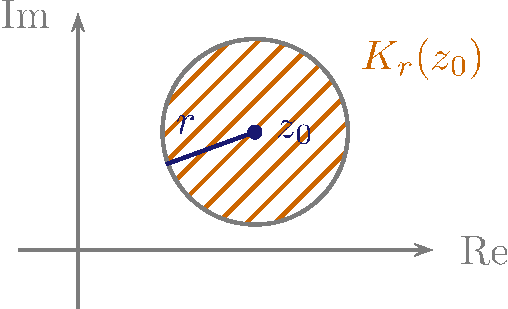
\includegraphics[scale=0.2]{images/ana3-tmp-22}
    \end{figure}

    \begin{enum-arab}
      \item \label{itm:2.24 1} Zeige $T > a$

      \item \label{itm:2.24 2} Zeige $T = b$ (Dann $f(z) = f(z_0) \, \forall \, z \in G$)
    \end{enum-arab}

    Zu \ref{itm:2.24 1}
    %
    \begin{align*}
      f(z) &\overset{\text{\ref{thm:2.7}}}{\underset{\text{\ref{thm:2.10}}}{=}} \sum\limits_{n=0}^{\infty} \frac{f^{(n)}(z_0)}{n!} (z-z_0)^n \quad \text{für } |z-z_0| < R \\
      &= f(z_0)
    \end{align*}
    %
    $\gamma$ stetig $\implies$ $\exists \, \delta > 0 \, \forall \, t \in [a,a+\delta[ : |\gamma(t) - \underbrace{\gamma(a)}_{=z_0}| < R$

    $\implies$ $T \geq a + \delta > a$

    Zu \ref{itm:2.24 2}: Annahme: $T < b$. Behauptung
    %
    \begin{align*}
      f^{(n)} (\gamma(t)) = 0 \quad \text{für } n \in \mathbb{N}, a \leq t \leq T
    \end{align*}
    %
    Induktionsanfang:
    %
    \begin{align*}
      f'(\gamma(t)) &= \lim\limits_{z \to \gamma(t)} \frac{f(z) - f(\gamma(t))}{z - \gamma(t)} \\
      &\overset{\text{Teilfolge}}{=} \lim\limits_{\substack{s \to t}{s \in [a,T]}} \frac{f(\gamma(s)) - f(\gamma(t))}{\gamma(s) - \gamma(t)} \overset{f|_{[a,T]}}{=} 0
    \end{align*}
    %
    Induktionsschritt genauso.

    $\implies$ $\forall \, n \in \mathbb{N} : f^{(n)}(\gamma(T)) = 0$

    $\overset{\text{wie \ref{itm:2.24 1}}}{\implies}$ $f(z) = f(\gamma(T)) = f(z_0)$ für $|z-\gamma(T)| < R$
  \end{proof}
\end{theorem}

%
% vim: ts=2:sw=2:expandtab
% Henri Menke, 2012 Universität Stuttgart.
%
% Dieses Werk ist unter einer Creative Commons Lizenz vom Typ
% Namensnennung - Nicht-kommerziell - Weitergabe unter gleichen Bedingungen 3.0 Deutschland
% zugänglich. Um eine Kopie dieser Lizenz einzusehen, konsultieren Sie
% http://creativecommons.org/licenses/by-nc-sa/3.0/de/ oder wenden Sie sich
% brieflich an Creative Commons, 444 Castro Street, Suite 900, Mountain View,
% California, 94041, USA.

\section{Nullstellen}
\addtocounter{thmn}{1}
\setcounter{theorem}{0}

% % % Vorlesung vom 8.11.2012

\begin{theorem}[Defintion]
  Sei $O \to \mathbb{C}$ offen, $f$ holomorph in $O$, $z_0 \in O$, $f(z_0)=0$. Falls
  %
  \begin{align*}
    \exists \, k \in \mathbb{N} : f^{(k)}(z_0) \neq 0
  \end{align*}
  %
  so heißt
  %
  \begin{align*}
    K \coloneq \min \{ k \in \mathbb{N} : f^{(k)}(z_0) \neq 0 \}
  \end{align*}
  %
  die \acct{Ordnung} oder \acct{Vielfachheit} der Nullstelle $z_0$. Andernfalls heißt die Ordnung der Nullstelle unendlich.
\end{theorem}

Betrachte:
%
\begin{align*}
  f : \mathbb{C} \to \mathbb{C} : z \mapsto z^2 : r \mathrm{e}^{\mathrm{i} \varphi} \mapsto r^2 \mathrm{e}^{2 \mathrm{i} \varphi}
\end{align*}

\begin{figure}[H]
  \centering
  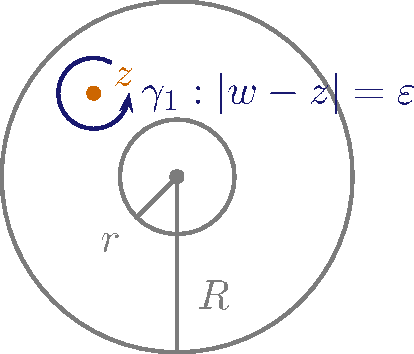
\includegraphics[scale=0.2]{images/ana3-tmp-23}
\end{figure}

Offensichtlich ist $f$ nicht injektiv. Jedes Element $w \neq 0$ hat genau zwei Urbilder.

Abhilfe: \acct{Riemannsche Fläche}. Lege zwei $\mathbb{C} \setminus \{ 0 \}$ Ebenen übereinander, schneide sie jeweils an der positiven reellen Achse auseinander, verbinde den Rand für $\Im z \uparrow 0$ der unteren Ebene mit dem Rand $\Im z \downarrow 0$ der oberen, verbinde die beiden anderen Ränder. Dann ist die Funktion
%
\begin{align*}
  f : \mathbb{C} \setminus \{0\} \to F = \{ r \mathrm{e}^{\mathrm{i} \varphi} : r > 0, \varphi \in \mathbb{R}, \mathrm{e}^{\mathrm{i} \varphi + 2 \pi} \neq \mathrm{e}^{\mathrm{i} \varphi}, r \mathrm{e}^{\mathrm{i} \varphi + 4 \pi} = \mathrm{e}^{\mathrm{i} \varphi} \}
\end{align*}
%
bijektiv. Die Riemannsche Fläche hat zwei Blätter.

% % % Vorlesung vom 12.11.2012

\begin{example*}
  \begin{align*}
    f(z) = \sin z^2
  \end{align*}
  %
  Nullstelle bei $z=0$
  %
  \begin{align*}
    f'(0) &= 2 z \cos z^2 \Big|_{z=0} = 0 \\
    f''(0) &= 2 \cos z^2 - 4 z^2 \sin z^2 \Big|_{z=0} = 2
  \end{align*}
  %
  $z=0$ ist Nullstelle 2. Ordnung.
\end{example*}

\begin{notice*}[Ziel:]
  Ist $z_0$ Nullstelle der Ordnung $k \in \mathbb{N}$, so verhält sich $f$ und ihre >>Umkehrfunktionen<< lokal wie
  %
  \begin{align*}
    z \mapsto (z-z_0)^k
  \end{align*}
  %
  und ihre >>Umkehrfunktionen<<.
\end{notice*}

\begin{theorem}[Hilfssatz]
  Sei $0 \leq \varphi \leq 2 \pi$, $\mathbb{C}_{\varphi_0} \coloneq \{ r \mathrm{e}^{\mathrm{i} \varphi} : r > 0, -\pi + \varphi_0 < \varphi < \pi + \varphi_0 \}$ $=\mathbb{C} \setminus \{ r \mathrm{e}^{\mathrm{i} (\varphi_0 + \pi)} : r > 0 \}$

  \begin{figure}[H]
    \centering
    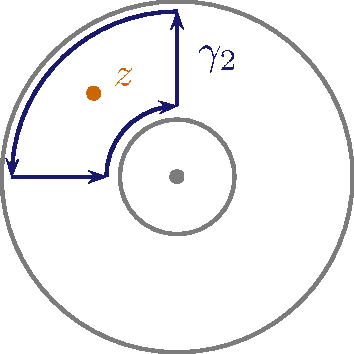
\includegraphics[scale=0.2]{images/ana3-tmp-24}
    \vspace*{-4em}
  \end{figure}

  \begin{align*}
    \arg_{\varphi_0} (z) \coloneq
    \begin{dcases}
      \arg z & -\pi + \varphi_0 < \arg z < \pi \\
      \arg z + 2 \pi & -\pi \leq \arg z < -\pi + \varphi_0
    \end{dcases}
  \end{align*}
  %
  Dann ist $\arg_{\varphi_0} : \mathbb{C}_{\varphi_0} \to ]-\pi+\varphi_0 , \pi+\varphi_0[$ stetig.

  \begin{proof}
    $z \mapsto 1/|z|$, $z \mapsto \Re z$, $z \mapsto \Im z$ sind stetig auf $\mathbb{C}_{\varphi_0}$.
    %
    \begin{align*}
      \arg_{\varphi_0} (z) =
      \begin{dcases}
        \arccos \frac{\Re z}{|z|} \; (\text{evtl. } + 2 \pi) & \text{für } \Im z \geq 0 \\
        \arcsin \frac{\Im z}{|z|} \; (\text{evtl. } + 2 \pi) & \text{für } \Re z \geq 0 \\
        2 \pi - \arccos \frac{\Re z}{|z|} \; (\text{evtl. } + 2 \pi) & \text{für } \Im z \leq 0
      \end{dcases}
    \end{align*}
    %
    Jede einzelne Zeile ist stetig und die Bereiche überlappen sich. Also ist $\arg_{\varphi_0}$ stetig auf der Vereinigung der einzelnen Bereiche.
  \end{proof}
\end{theorem}

\begin{theorem}[Satz]
  Sei $0 \leq \varphi_0 \leq 2 \pi$, $\sqrt[k]{\cdot} : \mathbb{C}_{\varphi_0} \to \mathbb{C}$ mit
  %
  \begin{align*}
    z^{1/k} \coloneq \sqrt[k]{z} \coloneq |z|^{1/k} \mathrm{e}^{\mathrm{i}\frac{1}{k}\arg_{\varphi_0}z}
  \end{align*}
  %
  Dann ist $\sqrt[k]{\cdot}$ holomorph und
  %
  \begin{align*}
    (\sqrt[k]{z})^k = z \qquad \sqrt[k]{z}' = \frac{1}{k (\sqrt[k]{z})^{k-1}}
  \end{align*}

  \begin{proof}
    \begin{enum-arab}
      \item $\sqrt[k]{\cdot}$ ist stetig als Kombination stetiger Funktionen

      \item $\sqrt[k]{\cdot}$ ist injektiv, denn
      %
      \begin{align*}
        (\sqrt[k]{z})^k = |z| \mathrm{e}^{\mathrm{i} \arg_{\varphi_0}z} = z
      \end{align*}

      \item Ableitung: Sei $z_0 \in \mathbb{C}_{\varphi_0}$, $f(z) \coloneq z^k$
      %
      \begin{align*}
        \sqrt[k]{z}'\Big|_{z=z_0} &= \lim\limits_{\substack{z \to z_0}{z \neq z_0}} \frac{\sqrt[k]{z} - \sqrt[k]{z_0}}{z-z_0} \\
        &\overset{g \coloneq \sqrt[k]{\cdot}}{=} \lim\limits_{\substack{z \to z_0}{z \neq z_0}} \frac{g(z) - g(z_0)}{z-z_0} \\
        &= \lim\limits_{\substack{z \to z_0}{z \neq z_0}} \frac{g(z) - g(z_0)}{f(g(z)) - f(g(z_0))} \\
        &= \lim\limits_{\substack{z \to z_0}{z \neq z_0}} \frac{1}{\frac{f(g(z)) - f(g(z_0))}{g(z) - g(z_0)}} \\
        &= \frac{1}{\lim\limits_{\substack{\zeta \to g(z_0)}{\zeta \neq g(z_0)}} \dfrac{f(\zeta) - f(g(z_0))}{\zeta - g(z_0)}} \\
        &= \frac{1}{f'(g(z_0))} \overset{f'(z)=k z^{k-1}}{=} \frac{1}{k (\sqrt[k]{z})^{k-1}}
      \end{align*}
    \end{enum-arab}
  \end{proof}
\end{theorem}

\begin{theorem}[Satz] \label{thm:3.4}
  Sei $O \subseteq \mathbb{C}$ offen, $f$ holomorph in $O$, $z_0 \in O$ Nullstelle der Ordnung $k \in \mathbb{N}$. Dann existiert $r > 0$ und eine holomorphe Funktion $h : K_r(z_0) \to \mathbb{C}$ mit
  %
  \begin{align*}
    h(z_0) = 0 \; , \quad h'(z_0) \neq 0 \; , \quad f(z) = h(z)^k \text{ für } |z-z_0| < r
  \end{align*}

  \begin{proof}
    O.B.d.A.\footnote{Ohne Bedenken des Autors}: $z_0 = 0$, und weil $f^{(j)}=0$, $j=0,\ldots,k-1$
    %
    \begin{align*}
      f(z) = \sum\limits_{n=k}^{\infty} a_n z^n = z^k \underbrace{\left( a_k + \sum\limits_{n=k+1}^{\infty} a_n z^{n-k} \right)}_{\eqcolon g(z)} \; , \quad \text{für } |z| < R
    \end{align*}
    %
    Dann ist $g$ holomorph in $K_r(0)$, $g(0) = a_k \neq 0$.

    \begin{figure}[H]
      \centering
      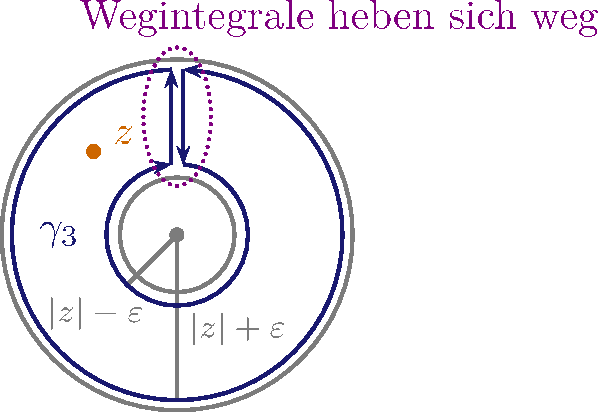
\includegraphics[scale=0.2]{images/ana3-tmp-25}
    \end{figure}

    Da $g$ stetig ist:
    %
    \begin{align*}
      \exists \, r > 0 : |z| < r \implies |g(z) - g(0)| < \frac{|g(0)|}{2}
    \end{align*}
    %
    Dann folgt:
    %
    \begin{align*}
      |z| < r \implies g(z) \in \mathbb{C}_{\arg g(0)}
    \end{align*}
    %
    Definiere
    %
    \begin{align*}
      h(z) \coloneq z \sqrt[k]{g(z)} \; , \quad \text{für } |z| < r
    \end{align*}
    %
    Dann:
    %
    \begin{align*}
      h(0) &= 0 \sqrt[k]{g(0)} = 0 \\
      h'(0) &= 1 \underbrace{\sqrt[k]{g(0)}}_{\neq 0} + 0 \frac{1}{k (\sqrt[k]{g(0)})^{k-1}} \neq 0
    \end{align*}
    %
    $h$ ist holomorph auf $K_r(0)$ als Produkt und Verkettung holomorpher Funktionen.
  \end{proof}
\end{theorem}

\begin{example}
  Sei $f : \mathbb{C} \to \mathbb{C} : z \mapsto \mathrm{e}^z$
  %
  \begin{align*}
    |f'(z)| &= |\mathrm{e}^z| = \left| \mathrm{e}^{\Re z + \mathrm{i} \Im z} \right| = \left| \mathrm{e}^{\Re z} \right| \left| \mathrm{e}^{\mathrm{i} \Im z} \right| \\
    &= \mathrm{e}^{\Re z} > 0
  \end{align*}
  %
  Trotzdem ist $f$ nicht injektiv:
  %
  \begin{align*}
    \mathrm{e}^{z + 2 \pi \mathrm{i}} = \mathrm{e}^z
  \end{align*}
\end{example}

\begin{theorem}[Lokale Umkehrfunktion] \label{thm:3.6}
  $f$ holomorph in $O$, $z_0 \in O$, $f'(z_0) \neq 0$. Dann existiert $r > 0$, sodass $f\Big|_{K_r(z_0)}$ injektiv ist. Weiter gelten
  %
  \begin{item-triangle}
    \item $f(K_r(z_0))$ ist offen

    \item $f^{-1} : f(K_r(z_0)) \to K_r(z_0)$ ist holomorph

    \item $(f^{-1}(w))' = \dfrac{1}{f'(f^{-1}(w))}$ für $w \in f(K_r(z_0))$
  \end{item-triangle}

  \begin{proof}
    Seien
    %
    \begin{align*}
      u(x,y) \coloneq \Re f(x+\mathrm{i}y) \\
      v(x,y) \coloneq \Im f(x+\mathrm{i}y)
    \end{align*}
    %
    Dann
    %
    \begin{align*}
      f(z) = w_1 + \mathrm{i} w_2 &\iff
      \begin{dcases}
        \Re f(x+\mathrm{i}y) = w_1 \\
        \Im f(x+\mathrm{i}y) = w_2
      \end{dcases}
      \\
      &\iff
      \begin{dcases}
        g_1(x,y,w_1,w_2) \coloneq u(x,y) - w_1 = 0 \\
        g_2(x,y,w_1,w_2) \coloneq v(x,y) - w_2 = 0
      \end{dcases}
    \end{align*}
    %
    Es gelten
    %
    \begin{enum-arab}
      \item $g_1,g_2 \in C^1(\cdot)$

      \item und
      %
      \begin{align*}
        \begin{vmatrix}
          \partial_x g_1 & \partial_y g_1 \\
          \partial_x g_2 & \partial_y g_2
        \end{vmatrix}
        &=
        \begin{vmatrix}
          u_x & u_y \\
          v_x & v_y
        \end{vmatrix}
        =
        \begin{vmatrix}
          \Re f' & -\Im f' \\
          \Im f' & \Re f'
        \end{vmatrix}
        \\
        &= |f'(z_0)|^2 \neq 0
      \end{align*}

      \item $g_j(x_0,y_0,\underbrace{\Re f(z_0)}_{u(x_0,y_0)},\underbrace{\Im f(z_0)}_{v(x_0,y_0)}) = 0$. Also $(x_0,y_0,\Re f(z_0),\Im f(z_0))$ ist eine Lösung.
      %
      \begin{theorem*}[Satz über implizite Funktionen]
        Es existiert eine Umgebung $\widetilde{U}$ von $(u(x_0,y_0),$ $v(x_0,y_0))$ % FIXME: Zeilenumbruch durch Leerzeichen erreicht
        im $\mathbb{R}^2$ und $\varphi_1,\varphi_2 \in C^1(\widetilde{U} \to \mathbb{R})$ mit
        %
        \begin{align*}
          g_j(\varphi_1(w_1,w_2),\varphi_2(w_1,w_2),w_1,w_2) = 0 \; , \quad j=1,2
        \end{align*}
        %
        und diese Lösungen sind eindeutig in einer Umgebung $\widetilde{V}$ von $(x_0,y_0)$.
      \end{theorem*}
      %
      Setze
      %
      \begin{align*}
        V \coloneq \{ x+\mathrm{i}y : x,y \in \widetilde{V} \}
        \implies
        \begin{dcases}
          f \Big|_{V} \text{ ist injektiv} \\
          f^{-1}(w_1,w_2) = \varphi_1(w_1,w_2) + \mathrm{i} \varphi_2(w_1,w_2) \\
          f^{-1} \text{ ist stetig, da } \varphi_1, \varphi_2 \text{ stetig}
        \end{dcases}
      \end{align*}
      %
      $\implies \exists \, r > 0 : K_r(z_0) \subseteq V$, da $V$ Umgebung von $z_0$. Wir wissen:
      %
      \begin{align*}
        f(f^{-1}(w)) &= w \\
        \implies
        (f^{-1}(w))' &= \lim\limits_{u \to w} \frac{f^{-1}(u) - f^{-1}(w)}{u - w} \\
        &= \lim\limits_{u \to w} \frac{1}{\frac{f(f^{-1}(u)) - f(f^{-1}(w))}{f^{-1}(u) - f^{-1}(w)}} = \frac{1}{f'(f^{-1}(w))}
      \end{align*}
    \end{enum-arab}
  \end{proof}
\end{theorem}

\begin{theorem}[Blätterzahl einer Nullstelle] \label{thm:3.7}
  Sei $f$ holomorph in $O$, $z_0 \in O$ Nullstelle der Ordnung $k \in \mathbb{N}$. Zu jedem genügend kleinen $\varepsilon > 0$ existiert eine offene Umgebung $O_\varepsilon$ von $z_0$ mit
  %
  \begin{align*}
    f(O_\varepsilon) = K_\varepsilon(0)
  \end{align*}
  %
  , sodass
  %
  \begin{align*}
    f\Big|_{O_\varepsilon} \text{ nimmt }
    \begin{dcases}
      \text{jeden Wert $w$ mit } 0 < |w| < \varepsilon \text{ genau $k$ Mal an} \\
      w=0 \text{ genau ein Mal an}
    \end{dcases}
  \end{align*}

  \begin{proof}
    \ref{thm:3.4} $\implies$ $f(z) = h(z)^k$, $h$ holomorph in $K_r(z_0)$ $h'(z_0) \neq 0$.

    \ref{thm:3.6} $\implies$ $h\Big|_{K_\delta(z_0)}$ injektiv, falls $\delta$ klein genug. Außerdem $h(K_\delta(z_0))$ offen. Wähle $\varepsilon > 0$ mit $K_\varepsilon(0) \subseteq h(K_\delta(z_0))$. Setze $O_\varepsilon \coloneq h^{-1}(K_\delta(z_0))$. Dann:

    \begin{figure}[H]
      \centering
      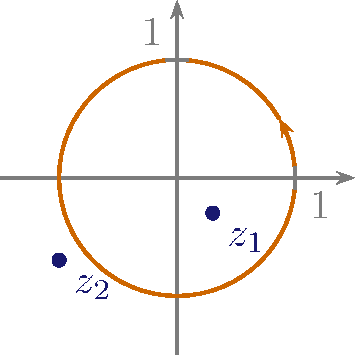
\includegraphics[scale=0.2]{images/ana3-tmp-26}
    \end{figure}
  \end{proof}
\end{theorem}

% % % Vorlesung vom 15.11.2012

\begin{notice}[Folgerung:] \label{thm:3.8}
  Nullstellen endlicher Ordnung sind isoloiert: Ist $f$ holomorph in $O$, $z_0 \in O$ Nullstelle endlicher Ordnung, so gilt:
  %
  \begin{align*}
    \exists \, \varepsilon \, \forall \, z \in K_\varepsilon(z_0) \setminus \{ z_0\} : f(z) \neq 0
  \end{align*}
\end{notice}

\begin{theorem}[Satz von der inversen Abbildung] \label{thm:3.9}
  Seien $O_1, O_2 \subseteq \mathbb{C}$ offen, $f : O_1 \to O_2$ holomorph und bijektiv. Dann
  %
  \begin{item-triangle}
    \item $f'(z) \neq 0$ in $O_1$

    \item $f^{-1}$ ist holomorph

    \item $\left(f^{-1}(w)\right)' = \dfrac{1}{f'(f^{-1}(w))}$
  \end{item-triangle}

  \begin{proof}
    Annahme: $\exists \, z_0 \in O_1 : f'(z_0) = 0$
    %
    \begin{align*}
      g(z) \coloneq f(z) - f(z_0)
    \end{align*}
    %
    Also ist $g$ holomorph und $z_0$ ist Nullstelle mindestens 2. Ordnung.

    \minisec{Fall 1: $z_0$ ist Nullstelle endlicher Ordnung}

    $\overset{\text{\ref{thm:3.7}}}{\implies}$ $g$ ist nicht injektiv.

    $\implies$ $f$ ist nicht injektiv. $\lightning$

    \minisec{Fall 2: $z_0$ ist Nullstelle der Ordnung $\infty$}

    $\overset{\text{\ref{thm:2.24}}}{\implies}$ $g = \mathrm{const.}$ in $K_\varepsilon(z_0) \subseteq O_1$.

    $\implies$ $f = \mathrm{const.}$ in $K_\varepsilon(z_0) \subseteq O_1$. $\lightning$

    Rest aus \ref{thm:3.6}
  \end{proof}
\end{theorem}

\begin{theorem}[Identitätssatz] \label{thm:3.10}
  Sei $G \subseteq \mathbb{C}$ Gebiet, $f,g$ holomorph in $G$, $(z_n)$ Folge in $G$, $z_n \to z_0 \in G$, $z_n \neq z_0$ für $n \in \mathbb{N}$, $f(z_n) = g(z_n)$. Dann ist $f=g$ in $G$.

  \begin{proof}
    Sei $h \coloneq f - g$ in $G$. Dann gilt $h$ holomorph, $h(z_n) = 0$. Daraus folgt $h(z_0) = 0$. Wegen $h(z_n) = 0$, $z_n \to z_0$ und $z_n \neq z_0$ ist die Nullstelle $z_0$ nicht isoliert.

    $\overset{\text{\ref{thm:3.8}}}{\implies}$ $z_0$ ist Nullstelle der Ordnung $\infty$.

    $\overset{\text{\ref{thm:2.24}}}{\implies}$ $h = \mathrm{const.}$ in G und $h(z_0) = 0$ $\implies$ $h=0$ in $G$, also $f=g$ in $G$.
  \end{proof}
\end{theorem}

\begin{theorem}[Gebietstreue] \label{thm:3.11}
  $G \subseteq \mathbb{C}$ Gebiet, $f$ holomorph in $G$, $f \neq \mathrm{const.}$. Dann ist $f(G)$ ein Gebiet.

  \begin{proof}
    \begin{enum-arab}
      \item $f(G)$ ist wegzusammenhängend: Seien $w_j = f(z_j) \in f(G)$, $j=1,2$.
      %
      \begin{align*}
        \text{$G$ Gebiet }
        &\implies \text{ Es existiert ein Weg $\gamma$ in $G$ von $z_1$ nach $z_2$} \\
        &\implies \text{ $f \circ \gamma$ ist Weg von $w_1$ nach $w_2$ in $f(G)$}
      \end{align*}

      \item $f(G)$ ist offen: Sei $w_0 = f(z_0) \in f(G)$.
      %
      \begin{align*}
        g \coloneq f(z) - f(z_0) \; , \quad z \in G
      \end{align*}
      %
      $\implies$ $g$ holomorph, $z_0$ Nullstelle.

      \minisec{Fall 1: $z_0$ hat Ordnung $\infty$}

      $\overset{\text{\ref{thm:2.24}}}{\implies}$ $g = \mathrm{const.}$, also $f = \mathrm{const.}$. $\lightning$

      \minisec{Fall 2: $z_0$ hat endliche Ordnung $k \in \mathbb{N}$}

      $\overset{\text{\ref{thm:3.7}}}{\implies}$ $\exists \, O_\varepsilon \in G : K_\varepsilon(0) \subseteq \mathrm{Bild}(g)$

      $\implies$ $K_\varepsilon(f(z_0)) = f(z_0) \oplus K_\varepsilon(0) \subseteq \mathrm{Bild}(f)$

      $\implies$ $\exists \, \varepsilon > 0 : K_\varepsilon(w_0) \subseteq f(G)$
    \end{enum-arab}
  \end{proof}
\end{theorem}

\begin{theorem*}[Definition]
  $K$ ist kompakt, $\iff$
  %
  \begin{align*}
    \text{$\forall \, (O_i)_{i \in I}$ offenes Mengensystem } : K \subseteq \bigcup\limits_{i \in I} O_i \implies \exists \, i_1, \ldots, i_n \in J : K \subseteq \bigcup\limits_{j=1}^{n} O_{ij}
  \end{align*}

  $K$ ist folgenkompakt, $\iff$
  %
  \begin{align*}
    \forall \, (x_n) \text{ Folge in } K : \text{ Es existiert eine Teilfolge } (x_{n_k}) \text{ mit } x_{n_k} \to x \in K
  \end{align*}

  $H$ eine Borel $K \subseteq \mathbb{R}^n$, dann
  %
  \begin{align*}
    \text{$K$ kompakt }
    &\iff \text{ $K$ beschränkt und $K$ abgeschlossen} \\
    &\implies \text{ gilt immer} \\
    &\impliedby \text{ gilt nicht in $\infty$-dimensionalen Räumen}
  \end{align*}
\end{theorem*}

\begin{theorem}[Maximumprinzip I] \label{thm:3.12}
  Sei $G \subseteq \mathbb{C}$ ein Gebiet und $f$ holomorph in $G$. Falls ein $z_0 \in G$ existiert, so dass
  %
  \begin{align}
    \forall \, z \in G : |f(z)| \leq |f(z_0)| \label{eq:3.12stern1} \tag{$\ast$}
  \end{align}
  %
  oder
  %
  \begin{align*}
    f(z_0) \neq 0 \; \land \; \forall \, z \in G : |f(z)| \geq |f(z_0)|
  \end{align*}
  %
  (d.h. $f$ nimmt in $G$ das Maximum oder Minimum $\neq 0$ an) Dann gilt $f = \mathrm{const.}$ in $G$

  \begin{proof}
    Sei $|f(z)| \leq |f(z_0)|$ für alle $z \in G$ und $f$ nicht konstant.
    Nach \ref{thm:3.11} ist $f(G)$ ein Gebiet und insbesondere offen, es existiert also $\varepsilon > 0$ mit
    %
    \begin{align*}
      K_\varepsilon(f(z_0)) \subseteq f(G)
    \end{align*}
    %
    Wir finden jetzt anschaulich ein $w \in K_\varepsilon(f(z_0))$ mit $|w| > |f(z_0)|$.
    Da $w$ im Bild von $f$ liegt, existiert auch ein $z_1 \in G$ mit
    %
    \begin{align*}
      |f(z_1)| = |w| > |f(z_0)|
    \end{align*}
    %
    \begin{figure}[H]
      \centering
      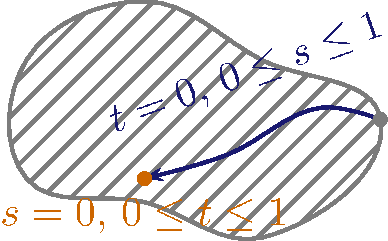
\includegraphics[scale=0.2]{images/ana3-tmp-27}
    \end{figure}
    %
    Das stellt ein Widerspruch zur Vorraussetzung dar.

    Den zweiten Fall behandelt man analog (die Forderung $f(z_0) \neq 0$ wird klar, weil man in diesem Fall keinen Widerspruch erzeugen kann).
  \end{proof}
\end{theorem}

\begin{theorem}[Maximumprinzip II] \label{thm:3.13}
  Sei $G \subseteq \mathbb{C}$ Gebiet, $G$ beschränkt, $f : \bar{G} \to \mathbb{C}$ stetig und $f$ holomorph in $G$. Dann
  %
  \begin{enum-arab}
    \item $\exists \, z_1 \in \partial G \, \forall \, z \in \bar{G} : |f(z)| \leq |f(z_1)|$

    \item Falls $\min\limits_{z \in \bar{G}} |f(z)| > 0$:
    %
    \begin{align*}
      \exists \, z_2 \in \partial G \, \forall \, z \in \bar{G}: |f(z)| \geq |f(z_2)|
    \end{align*}
  \end{enum-arab}

  \begin{proof}
    $\bar{G}$ ist kompakt und $|f| : \bar{G} \to \mathbb{R}$ stetig, also
    %
    \begin{align*}
      \exists \, z_1,z_2 \in \bar{G} \, \forall \, z \in \bar{G} : |f(z_2)| \leq |f(z)| \leq |f(z_1)|
    \end{align*}
    %
    Falls $z_1 \in \partial G$, sind wir schon fertig.
    Sei also $z_1 \in G$.
    Damit ist nach \ref{thm:3.12} $f$ konstant in $G$ und wegen der Stetigkeit auch in $\bar{G}$, also ist $z_1 \in \partial G$ wählbar. Genauso für $z_2$.
  \end{proof}
\end{theorem}

\begin{example}
  $f(z) = \mathrm{e}^z$, $G = K_2(1 + 2 \mathrm{i})$
  %
  \begin{figure}[H]
    \centering
    \psset{unit=0.7cm}
    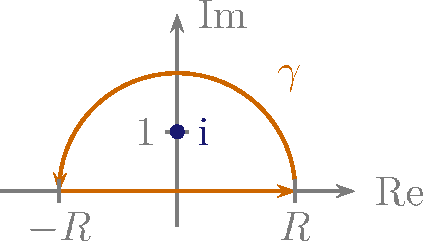
\includegraphics[scale=0.2]{images/ana3-tmp-28}
    \psset{unit=1cm}
    \vspace*{-4em}
  \end{figure}
  %
  \begin{align*}
    |f(z)| &= |\mathrm{e}^z| = \mathrm{e}^{\Re z} \\
    \implies \quad \mathrm{e}^{-1} &= |f(-1+2\mathrm{i})| \leq |f(z)| \leq \mathrm{e}^3 = |f(3+2\mathrm{i})|
  \end{align*}
\end{example}

\begin{theorem}[Satz]
  Sei $f : ]a,b[ \to \mathbb{R}$, $x_0 \in ]a,b[$, $f$ in $x_0$ (reell-) analytisch, d.h.
  %
  \begin{align*}
    f(x) = y_0 + \sum\limits_{n=K}^{\infty} a_n (x-x_0)^n \quad \text{für } |x-x_0| < r
  \end{align*}
  %
  ($r>0$, $a_n \in \mathbb{R}$, $K \in \mathbb{N}$, $a_K \neq 0$). Dann existiert ein $\varepsilon > 0$, sodass
  %
  \begin{align*}
    f_{+} \coloneq f \Big|_{[x_0,x_0+\varepsilon[} \qquad f_{-} \coloneq f \Big|_{]x_0-\varepsilon,x_0]}
  \end{align*}
  %
  injektiv sind, dass $f_{+}^{-1}$, $f_{-}^{-1}$ sind als \acct{Puiseux-Reihen} darstellbar.
  %
  \begin{align*}
    f_{\pm}^{-1}(y) = x_0 + \sum\limits_{n=1}^{\infty} b_n \left( \pm |y-y_0|^{1/K} \right)^n
    \quad \text{für } y \in
    \begin{dcases}
      f_{+}([x_0,x_0+\varepsilon[) \\
      f_{-}(]x_0-\varepsilon,x_0])
    \end{dcases}
  \end{align*}
  %
  ($b_n \in \mathbb{R}$, $b_1 = |a_K|^{-1/K} \neq 0$)

  Die Reihen für $f_{+}$ und $f_{-}$ haben dieselben Koeffizienten $b_n$. Einziger Unterschied: $+$ oder $-$ in $(\cdot)^n$.

  \begin{proof} % % % Vorlesung vom 19.11.2012
    O.B.d.A. $a_K > 0$. Sei
    %
    \begin{align*}
      g(z) &\coloneq \sum\limits_{n=K}^{\infty} a_n (z-x_0)^n \quad \text{für } |z-x_0| < r \\
      &\implies
      \begin{dcases}
        g \text{ holomorph} \\
        z = x_0 \text{ ist $K$-fache Nullstelle} \\
        y_0 + g(x) = f(x) \text{ für } x_0 - r < x < x_0 + r
      \end{dcases}
    \end{align*}
    %
    $\overset{\text{\ref{thm:3.4}}}{\implies}$ $g(z) = h(z)^K$ für $|z-x_0| < \varepsilon$, $h$ holomorph und $h'(x_0) \neq 0$.

    Aus dem Beweis von \ref{thm:3.4}:
    %
    \begin{align*}
      h(z) = (z-x_0) \underbrace{\left( \sum\limits_{n=K}^{\infty} a_n (z-x_0)^{n-K} \right){1/K}}_{=a_K > 0 \text{ für } z=x_0}
    \end{align*}
    %
    also $(\cdot)^{1/K} : \mathbb{C}_0 \to \mathbb{C}$, insbesondere $(\cdot)^{1/K} : [0,\infty[ \to \mathbb{R}$ ist die reelle $K$-te Wurzel.
    %
    \begin{align*}
      &\implies
      \begin{dcases}
        h^{-1} \text{ holomorph nach \ref{thm:3.6}} \\
        h(x) \in \mathbb{R} \text{ für } x_0-\varepsilon < x < x_0+\varepsilon \\
        h'(x_0) = 1 \cdot a_K^{1/K} + 0 \cdot \ldots = a_K^{1/K} > 0 \\
        \implies h \text{ streng monoton wachsend in } ]x_0-\varepsilon',x_0+\varepsilon'[ \text{ und reell} \\
        \implies h^{-1} \text{ streng monoton wachsend und reell}
      \end{dcases} \\
      &\implies
      \begin{dcases}
        h^{-1}(z) = x_0 + \sum\limits_{n=1}^{\infty} b_n \, z^n \text{ für } |z-x_0| < r' \\
        b_1 = \frac{{h^{-1}}'(0)}{1!} = \frac{1}{h'(x_0)} = \frac{1}{a_K^{1/K}} \\
        b_n \in \mathbb{R} \text{, da } b_n = \frac{1}{n!} \frac{\mathrm{d}^n h^{-1}}{\mathrm{d}x^n}(x_0) = \text{reeller Ableitung von } h^{-1}\Big|_{]x_0-r',x_0+r'[}
      \end{dcases} \\
    \end{align*}
    %
    Also:
    \begin{gather*}
      \begin{aligned}
        f(x) = y
        &\iff g(x) = y-y_0 \\
        &\iff h(x)^K = y-y_0 \\
      \end{aligned} \\
      \implies
      \left\{
      \begin{aligned}
        &x \geq x_0 : h(x) \geq h(x_0) = 0 \implies y \geq y_0 \\
        &\qquad \implies h(x) = (y-y_0)^{1/K} \\
        &\qquad \implies x = h^{-1} (y-y_0)^{1/K} = \underbrace{x_0 + \sum\limits_{n=1}^{\infty} b_n \left( (y-y_0)^{1/K} \right)^n}_{\eqcolon f_{+}^{-1}} \\
        &x \leq x_0 : h(x) \leq h(x_0) = 0 \implies y \leq y_0 \\
        &\qquad \implies h(x) = - |y-y_0|^{1/K} \\
        &\qquad \implies x = h^{-1}\left(-|y-y_0|^{1/K}\right) = \underbrace{x_0 + \sum\limits_{n=1}^{\infty} b_n \left( -|y-y_0|^{1/K} \right)^n}_{\eqcolon f_{-}^{-1}}
      \end{aligned}
      \right.
    \end{gather*}
  \end{proof}
\end{theorem}

\begin{example}
  $f(x) = c (x-x_0)^4$, $x \in \mathbb{R}$
  %
  \begin{figure}[H]
    \centering
    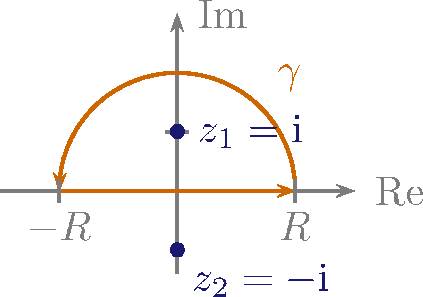
\includegraphics[scale=0.2]{images/ana3-tmp-29}
    \vspace*{-4em}
  \end{figure}
  %
  \minisec{Fall $c<0$:}
  %
  \begin{gather*}
    f_{+} : [x_0,\infty[ \to ]-\infty,0] \\
    f_{+}^{-1}(y) = x_0 + \left| \frac{y}{c} \right|^{1/4} \\
    f_{-} : ]-\infty,x_0] \to ]-\infty,0] \\
    f_{-}^{-1}(y) = x_0 - \left| \frac{y}{c} \right|^{1/4}
  \end{gather*}
  %
  Für $c<0$ dieselben Abbildungsvorschriften für $f_{+}^{-1}$, $f_{-}^{-1}$.
\end{example}

%
% vim: ts=2:sw=2:expandtab
% Henri Menke, 2012 Universität Stuttgart.
%
% Dieses Werk ist unter einer Creative Commons Lizenz vom Typ
% Namensnennung - Nicht-kommerziell - Weitergabe unter gleichen Bedingungen 3.0 Deutschland
% zugänglich. Um eine Kopie dieser Lizenz einzusehen, konsultieren Sie
% http://creativecommons.org/licenses/by-nc-sa/3.0/de/ oder wenden Sie sich
% brieflich an Creative Commons, 444 Castro Street, Suite 900, Mountain View,
% California, 94041, USA.

\section{Integrale längs geschlossener Kurven}
\addtocounter{thmn}{1}
\setcounter{theorem}{0}

% % % Vorlesung vom 19.11.2012

\begin{example}
  \begin{align*}
    f(z) &= \sum\limits_{n=0}^{\infty} a_n \, z^n \quad \text{für } |z| < r \\
    g(z) &= \sum\limits_{n=1}^{\infty} b_n \, z^n \quad \text{für } |z| < R \, , \; \frac{1}{R} < r
  \end{align*}
  %
  \begin{notice*}[Nebenrechnung:]
    $\left| \dfrac{1}{z} \right| < R \iff |z| > \dfrac{1}{R}$
  \end{notice*}
  %
  Sei $h(z) \coloneq f(z) + g(1/z)$
  %
  \begin{align*}
    \implies
    \begin{dcases}
      h \text{ holomorph im Kreisring } \frac{1}{R} < |z| < r \\
      \text{Für } \frac{1}{R} < |z| < r \text{ gilt } h(z) = \sum\limits_{n=-\infty}^{\infty} c_n \, z^n
      \text{ mit } c_n =
      \begin{cases}
        a_n & n \geq 0 \\
        b_n & n \leq -1
      \end{cases}
    \end{dcases}
  \end{align*}
\end{example}

\begin{theorem}[Laurent-Entwicklung] \index{Laurent-Entwicklung} \label{thm:4.2}
  Sei $0 \leq r < R$ und
  %
  \begin{align*}
    K_{r,R}(z_0) \coloneq \{ z \in \mathbb{C} : r < |z-z_0| < R \}
  \end{align*}
  %
  und $f$ holomorph in $K_{r,R}(z_0)$. Dann ist $f$ als \acct{Laurent-Reihe} darstellbar.
  %
  \begin{align*}
    f(z) \coloneq \sum\limits_{n=-\infty}^{\infty} a_n (z-z_0)^n \quad \text{für } z \in K_{r,R}(z_0)
  \end{align*}
  %
  wobei
  %
  \begin{align*}
    a_n = \frac{1}{2 \pi \mathrm{i}} \int\limits_{|z-z_0| = \varrho} \frac{f(z)}{(z-z_0)^{n+1}} \mathrm{d}z \quad \text{für } r < \varrho < R
  \end{align*}
  %
  (\acct{Cauchy-Formel für Laurent-Koeffizienten}).
  %
  \begin{align*}
    H(z) \coloneq \sum\limits_{n=-1}^{-\infty} a_n (z-z_0)^n
  \end{align*}
  %
  heißt \acct[0]{Hauptteil},
  %
  \begin{align*}
    N(z) \coloneq \sum\limits_{n=0}^{\infty} a_n (z-z_0)^n
  \end{align*}
  %
  heißt \acct[0]{Nebenteil} der Laurent-Reihe.
\end{theorem}

\begin{notice}
  \begin{enum-arab}
    \item $r=0$ ist erlaubt. Dann hat $f$ in $z_0$ eine isolierte Singularität (siehe unten). Riemannscher Hebbarkeitssatz: Entweder ist $f$ beschränkt bei $z_0$, dann ist es holomorph fortsetzbar in $z_0$, oder $f$ ist unbeschränkt für $z \to z_0$.

    Im ersten Fall sei $\widetilde{f}$ die holomorphe Fortsetzung. Für $n<0$ gilt dann
    %
    \begin{align*}
      a_n &= \frac{1}{2 \pi \mathrm{i}} \int\limits_{|z-z_0|=\varrho} \underbrace{f(z) \, (z-z_0)^{-n-1}}_{\text{holomorph in }K_{r,R}(z_0)} \, \mathrm{d}z = 0
    \end{align*}
    %
    Damit ist der Hauptteil der Laurentreihe $H(z) = 0$.

    \item $N(z)$ konvergiert immer im ganzen äußeren Kreis $K_{R}(z_0)$. $H(z)$ konvergiert immer außerhalb des inneren Kreises: $\{z \in \mathbb{C} : |z-z_0| > r \} = \mathbb{C} \setminus \overline{K_r(z_0)}$.
  \end{enum-arab}
\end{notice}

\begin{proof}[Beweis von \ref{thm:4.2}]
  O.B.d.A. $z_0 = 0$.
  Sei $z$ aus $K_{r,R}(0)$ fest, $\varepsilon \coloneq \dfrac{1}{2} \min \{ R - |z|, |z| - r\}$
  %
  \begin{figure}[H]
    \centering
    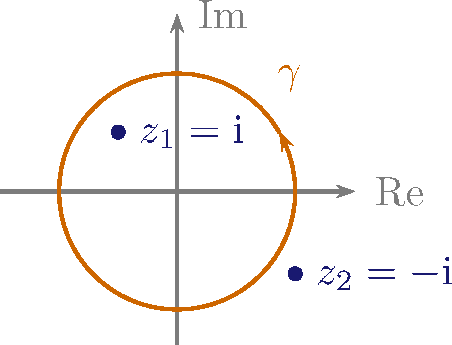
\includegraphics[scale=0.2]{images/ana3-tmp-30}
    \hspace*{2em}
    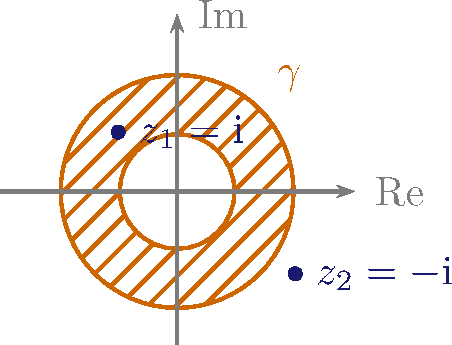
\includegraphics[scale=0.2]{images/ana3-tmp-31}
    \hspace*{2em}
    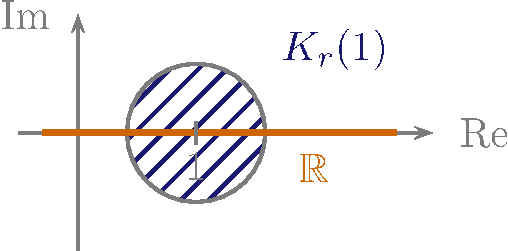
\includegraphics[scale=0.2]{images/ana3-tmp-32}
  \end{figure}
  %
  Es gilt: $\gamma_1 \sim \gamma_2 \sim \gamma_3$ in $K_{r,R}(0) \setminus \{z\}$.

  Cauchyscher Integralsatz (\ref{thm:2.4})
  %
  \begin{align*}
    f(z)
    &= \frac{1}{2 \pi \mathrm{i}} \int_{|w-z|=\varepsilon} \frac{f(w)}{w-z} \, \mathrm{d}w = \frac{1}{2 \pi \mathrm{i}} \int_{\gamma_3} \frac{f(w)}{w-z} \, \mathrm{d}w
  \intertext{Weil der innere Weg in mathematisch negativer Richtung durchlaufen wird erhält das zugehörige Interal ein negatives Vorzeichen}
    &= \frac{1}{2 \pi \mathrm{i}} \int_{|w|=|z|+\varepsilon} \frac{f(w)}{w-z} \, \mathrm{d}w - \frac{1}{2 \pi \mathrm{i}} \int_{|w|=|z|-\varepsilon} \frac{f(w)}{w-z} \, \mathrm{d}w \\
    &= \frac{1}{2 \pi \mathrm{i}} \int_{|w|=|z|+\varepsilon} \frac{f(w)}{w} \, \underbrace{\frac{1}{1 - \frac zw}}_{\mathclap{= \sum\limits_{n=0}^{\infty} (z/w)^n \text{ gleichmäßig}}} \, \mathrm{d}w
    - \frac{1}{2 \pi \mathrm{i}} \int_{|w|=|z|-\varepsilon} \frac{f(w)}{-z} \, \underbrace{\frac{1}{1 - \frac wz}}_{\mathclap{= \sum\limits_{n=0}^{\infty} (w/z)^n \text{ gleichmäßig}}} \, \mathrm{d}w
  \intertext{Vertausche Integral und Summe}
    &= \sum\limits_{n=0}^{\infty} \frac{1}{2 \pi \mathrm{i}} \int_{|w|=|z|+\varepsilon=\varrho} \frac{f(w)}{w^{n+1}} \, \mathrm{d}w \, z^n
    + \sum\limits_{n=0}^{\infty} \frac{1}{2 \pi \mathrm{i}} \int_{|w|=|z|-\varepsilon=\varrho} \frac{f(w)}{w^{-n}} \, \mathrm{d}w \, z^{-n-1} \\
    &= \sum\limits_{n=0}^{\infty} \underbrace{\frac{1}{2 \pi \mathrm{i}} \int_{\varrho} \frac{f(w)}{w^{n+1}} \, \mathrm{d}w}_{= a_n \text{ für } n \in \mathbb{N}} \, z^n
    + \sum\limits_{k=-1}^{-\infty} \underbrace{\frac{1}{2 \pi \mathrm{i}} \int_{\varrho} \frac{f(w)}{w^{k+1}} \, \mathrm{d}w}_{= a_k \text{ für } -k \in \mathbb{N}} \, z^k \\
  \end{align*}
\end{proof}

\begin{theorem}[Definition]
  \begin{enum-arab}
    \item Sei $O \subseteq \mathbb{C}$ offen, $f$ holomorph in $O$. Dann hat $f$ in $z_0 \in \mathbb{C} \setminus O$ eine \acct{isolierte Singularität}, falls
    %
    \begin{align*}
      \exists \, r > 0 : K_{0,r}(z_0) \subseteq O
    \end{align*}
    %
    (mit anderen Worten: einzig $z_0$ ist nicht in $O$ enthalten und $z_0$ ist komplett umhüllt von $O$)

    \item $f$ habe in $z_0$ eine isolierte Singularität. Nach \ref{thm:4.2} gilt
    %
    \begin{align*}
      f(z) = \sum\limits_{n = -\infty}^{\infty} a_n \, (z-z_0)^n \quad \text{in } K_{0,r}(z_0)
    \end{align*}
    %
    \begin{enum-alph}
      \item Falls $H(z) = 0$, d.h. $a_n = 0$ für $n \leq -1$, heißt die Singularität \acct[0]{hebbar}. \index{hebbare Singularität}

      \item Falls $H(z)$ nur endlich viele Summanden hat und $H \neq 0$, also
      %
      \begin{align*}
        \exists \, N \leq -1 : \big( a_N \neq 0 \land \, \forall \, n < N : a_n = 0 \big)
      \end{align*}
      %
      dann heißt $z_0$ \acct{Polstelle},
      %
      \begin{align*}
        K \coloneq - \min \{ n \in \mathbb{Z} : a_n \neq 0 \}
      \end{align*}
      %
      heißt \acct{Ordnung des Pols}.

      \item Falls $H$ unendlich viele Summanden hat
      %
      \begin{align*}
        \forall \, N \in \mathbb{Z} \, \exists \, n < N : a_n \neq 0
      \end{align*}
      %
      hat $f$ in $z_0$ eine \acct{wesentliche Singularität}
    \end{enum-alph}
  \end{enum-arab}
\end{theorem}

\begin{example}
  \begin{enum-arab}
    \item Sei $\varrho = \mathbb{C} \setminus \{ 0 \}$, \[ f : O \to \mathbb{C} : z \mapsto \mathrm{e}^{1/z} = \sum\limits_{n=0}^{\infty} \frac{1}{n!} z^{-n} \] hat wesentliche Singularität in $z_0 = 0$.

    \item Sei $f(z) \coloneq \dfrac{p(z)}{q(z)}$ wobei $p,q$ Polynome sind. Vereinfachungen:
    %
    \begin{enum-arab}
      \item $\mathrm{Grad}(p) < \mathrm{Grad}(q)$, sonst Polynomdivision

      \item Seien $z_1,\ldots,z_n$ Nullstellen von $q$. Es soll $p(z_j)\neq 0$ sein ($j=1,\ldots,n$), sonst gemeinsame Faktoren kürzen, eventuell holomorph ergänzen.
    \end{enum-arab}
    %
    Partialbruchzerlegung:
    %
    \begin{align*}
      &q(z) = (z-z_1)^K \widetilde{q}(z) \quad \widetilde{q}(z) \neq 0 \\
      \implies \quad &f(z) = \underbrace{\sum\limits_{n=1}^{\infty} \frac{c_j}{(z-z_1)^n}}_{\mathclap{\text{Hauptteil der Laurent-Reihe}}} + \frac{\widetilde{p}(z)}{\widetilde{q}(z)} \quad \text{mit } \mathrm{Grad}(\widetilde{p}) < \mathrm{Grad}(\widetilde{q}) \\
      \implies \quad &f \text{hat in $z_1$ einen Pol der Ordnung $K$}
    \end{align*}
  \end{enum-arab}
\end{example}

% % % Vorlesung vom 22.11.2012

\begin{notice}
  $f$ hat genau dann in $z_0$ einen Pol der Ordnung $K$, falls
  %
  \begin{align*}
    f(z) &= \sum\limits_{n=-K}^{\infty} a_n (z-z_0)^n = \frac{1}{(z-z_0)^K} \underbrace{\sum\limits_{n=-K}^{\infty} a_n (z-z_0)^{n+K}}_{= g(z)}
  \end{align*}
  %
  das heißt, falls
  %
  \begin{align*}
    f(z) &= \frac{1}{(z-z_0)^K} g(z)
  \end{align*}
  %
  $g$ holomorph in $K_\varepsilon(z_0)$ und $g(z) \neq 0$, weil $a_{-K} \neq 0$

  $\implies$ Falls $f$ in $z_0$ einen Pol der Ordnung $K \geq 1$ hat, gilt
  %
  \begin{align*}
    |f(z)| = \frac{1}{|z-z_0|^K} |g(z)| \to \infty \text{ für } z \to z_0
  \end{align*}
\end{notice}

\begin{theorem}[Casorati-Weierstraß-Sokhotski]
  Hat $f$ in $z_0$ eine wesentliche Singularität, so ist $f(K_{0,\varepsilon}(z_0))$ dicht in $\mathbb{C}$ sobald $\varepsilon$ so klein, dass $f$ auf ganz $K_{0,\varepsilon}(z_0)$ definiert ist, dann für alle solchen $\varepsilon > 0$.
  %
  \begin{proof}
    Sei so ein $\varepsilon > 0$ fest. Annahme:
    %
    \begin{align*}
      \exists \, w \in \mathbb{C} \, \exists \, \delta > 0 : K_\delta(w) \in \mathbb{C} \setminus f(K_{0,\varepsilon}(z_0))
    \end{align*}
    %
    Sei
    %
    \begin{gather*}
      g(z) \coloneq \frac{1}{f(z) - w} \; , \quad z \in K_{0,\varepsilon}(z_0) \\
      \implies
      \begin{dcases}
        g \text{ holomorph} \\
        g \text{ beschränkt } |g(z)| = \frac{1}{|f(z) - w|} < \frac{1}{\delta}
      \end{dcases}
    \end{gather*}
    %
    Riemannscher Hebbarkeitssatz: $g$ fortsetzbar zu $\widetilde{g} : K_\varepsilon(z_0) \to \mathbb{C}$ holomorph.

    \minisec{Fall 1:}

    \begin{align*}
      \widetilde{g}(z_0) \neq 0
      &\implies \dfrac{1}{\widetilde{g}} \text{ holomorph in } K_{\widehat{\varepsilon}}(z_0) \\
      &\implies f(z) = \frac{1}{\widetilde{g}(z)} + w \text{ holomorph fortsetzbar in } z = z_0 \\
      &\implies H = 0 \; \lightning
    \end{align*}

    \minisec{Fall 2:}

    $\widetilde{g}(z_0) = 0$, $K$ Ordnung der Nullstelle

    \begin{enum-alph}
      \item $K = \infty$: Dann $\widetilde{g} = 0$ in $K_\varepsilon(z_0)$ $\lightning$ $\widetilde{g}(z)=\dfrac{1}{f(z)-w} \neq 0$ für $z \in K_{0,\varepsilon}(z_0)$

      \item $K \in \mathbb{N}$:
      %
      \begin{align*}
        \widetilde{g}(z_0)
        &= \sum\limits_{n=-K}^{\infty} a_n (z-z_0)^n \; , \quad |z-z_0| < \varepsilon \\
        &= (z-z_0)^K \sum\limits_{n=K}^{\infty} a_n (z-z_0)^{n-K} \\
        &= (z-z_0)^K h(z) \; , \quad h \text{ holomorph}, h(z_0) \neq 0 \\
        \implies \quad \frac{1}{\widetilde{g}(z)} &= \frac{1}{(z-z_0)^K} \frac{1}{h(z)} \text{ für } 0 < |z-z_0| < \widetilde{\varepsilon} \\
        \implies \quad f(z) &= \frac{1}{\widetilde{g}(z)} + w \text{ hat Pol der Ordnung $K$ in $z_0$ $\lightning$}
      \end{align*}
    \end{enum-alph}
  \end{proof}
\end{theorem}

\begin{notice}[Folgerung:] \label{thm:4.8}
  $f$ hat Pol in $z_0$ $\iff$ $|f(z)| \to \infty$ für $z \to z_0$. $f$ hat wesentliche Singularität in $z_0$
  %
  \begin{itemize}
    \item[$\iff$] $f(K_\varepsilon(z_0))$ ist dicht in $\mathbb{C}$ für jedes genügend kleine $\varepsilon > 0$

    \item[$\iff$] $|f(z)|$ unbeschränkt, aber nicht bestimmt divergent
    \footnote{
      $|f(z)|$ bestimmt divergent für $z-z_0$
      \begin{itemize}
        \item[$\iff$] $|f(z)| \to \infty$
        \item[$\iff$] $\forall \, M > 0 \, \exists \, \delta > 0 : |z-z_0| < \delta \implies |f(z)| > M$
      \end{itemize}
    }
    für $z \to z_0$
  \end{itemize}
  %
  $f$ hat hebbare Singularität in $z_0$ $\iff$ $|f|$ beschränkt für $z \to z_0$
\end{notice}

\begin{theorem}[Definition]
  Sei $\gamma$ geschlossener Weg, $z_0 \in \mathbb{C} \setminus \mathrm{Bild}(\gamma)$. Dann heißt
  %
  \begin{align*}
    \nu(\gamma,z_0) \coloneq \frac{1}{2 \pi \mathrm{i}} \int_\gamma \frac{1}{z-z_0} \, \mathrm{d}z
  \end{align*}
  %
  die \acct{Umlaufszahl} von $\gamma$ um $z_0$.
\end{theorem}

\begin{theorem}[Satz]
  $\nu(\gamma,z_0) \in \mathbb{Z}$

  \begin{proof}
    $\nu(\gamma,z_0) \in \mathbb{Z} \iff \mathrm{e}^{2 \pi \mathrm{i} \nu(\gamma,z_0)}$. Sei
    %
    \begin{align*}
      \varphi(s) \coloneq \exp\left( \int\limits_{a}^{s} \frac{1}{\gamma(t) - z_0} \gamma'(t) \, \mathrm{d}t \right) \; , \quad (\gamma:[a:b] \to \mathbb{C})
    \end{align*}
    %
    Zeige $\varphi(b) = 1$.
    %
    \begin{align*}
      &&\varphi'(s) &= \varphi(s) \frac{1}{\gamma(s) - z_0} \gamma'(s) \; , \quad \text{ für } s \in [a,b] \setminus \{ t_0,\ldots,t_n \} \\
      &\implies& \frac{\mathrm{d}}{\mathrm{d}s} \left( \frac{\varphi(s)}{\gamma(s) - z_0} \right)
      &= \frac{\varphi' \, (\gamma - z_0) - \varphi \, \gamma'}{(\gamma - z_0)^2} = 0 \; , \quad \text{ für } s \in [a,b] \setminus \{ t_0,\ldots,t_n \} \\
      &\implies& \frac{\varphi(s)}{\gamma(s) - z_0} &= \mathrm{const} \text{ auf Teilintervallen}
    \intertext{es existieren nur endliche viele Teilintervalle und $\dfrac{\varphi(s)}{\gamma(s) - z_0}$ ist stetig}
      &\implies& \frac{\varphi(s)}{\gamma(s) - z_0} &= \mathrm{const} \text{ auf } [a,b] \\
      &&&= \frac{\varphi(a)}{\gamma(a) - z_0} \\
      &&&= \frac{1}{\gamma(a) - z_0} \\
      &\overset{s = b}{\implies}& \varphi(b) &= \frac{\gamma(b) - z_0}{\gamma(a)-z_0} = 1 \quad \text{da } \gamma(a)=\gamma(b)
    \end{align*}
  \end{proof}
\end{theorem}

\begin{example}
  \begin{enum-arab}
    \item $\gamma_N : [0,N] \to \mathbb{C} : t \mapsto \mathrm{e}^{2 \pi \mathrm{i} t}$
    %
    \begin{figure}[H]
      \centering
      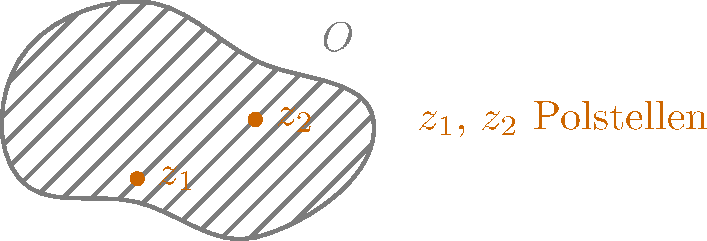
\includegraphics[scale=0.2]{images/ana3-tmp-33}
    \end{figure}
    %
    $\nu(\gamma_N,0) = N$ $\implies$ $\nu(-\gamma_N,0) = -N$

    $\nu(\gamma_N,z_1) = N$ falls $|z_1| < 1$ ($\gamma_N \overset{\text{in } \mathbb{C}\setminus\{z_1\}}{\sim} \widetilde{g}_N : t \mapsto z_1 + \mathrm{e}^{2 \pi \mathrm{i} t}$, dasselbe Integral)

    $\nu(\gamma_N,z_2) = 0$ falls $|z_2| > 1$, da $\gamma_N$ nullhomotop in $\mathbb{C} \setminus \{z_2\}$

    \item
    %
    \begin{figure}[H]
      \centering
%      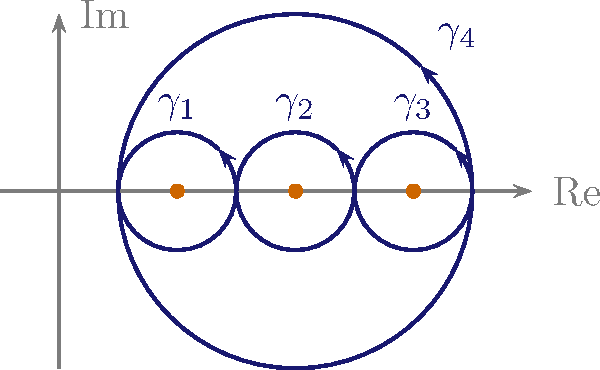
\includegraphics[scale=0.2]{images/ana3-tmp-34}
    \end{figure}
    %
    \begin{align*}
      \nu(\gamma,z_j) =
      \begin{dcases}
        0 & j = 3 \\
        1 & j = 1 \\
        -1 & j = 2 \\
      \end{dcases}
    \end{align*}
  \end{enum-arab}
\end{example}

\begin{theorem}[Satz] \label{thm:4.12}
  Sei
  %
  \begin{align*}
    f(z) = \sum\limits_{n = -\infty}^{\infty} a_n (z-z_0)^n \; , \quad 0 < |z-z_0| < R
  \end{align*}
  %
  und $\gamma$ geschlossener Weg in $K_{0,R}(z_0)$. Dann
  %
  \begin{align*}
    \int_{\gamma} f(z) \, \mathrm{d}z = 2 \pi \mathrm{i} a_{-1} \nu(\gamma,z_0)
  \end{align*}

  \begin{proof}
    \begin{align*}
      g(z)
      &\coloneq f(z) - a_{-1} (z-z_0)^{-1} \\
      &\coloneq \sum\limits_{\substack{n=-\infty}{n \neq -1}}^{\infty} a_n (z-z_0)^n
    \end{align*}
    %
    Dann ist
    %
    \begin{align*}
      G(z) \coloneq \sum\limits_{\substack{n=-\infty}{n \neq -1}}^{\infty} \frac{a_n}{n+1} (z-z_0)^{n+1}
    \end{align*}
    %
    eine Stammfunktion in $K_{0,R}(z_0)$
    %
    \begin{align*}
      \implies \quad \int_\gamma g(z) \, \mathrm{d}z &= G(\text{Endpunkt}) - G(\text{Anfangspunkt}) = 0 \\
      \implies \quad \int_\gamma f(z) \, \mathrm{d}z &= \underbrace{\int_\gamma g(z) \, \mathrm{d}z}_{=0} + a_{-1} \underbrace{\int_\gamma (z-z_0)^{-1} \, \mathrm{d}z}_{= \nu(\gamma,z_0) 2 \pi \mathrm{i}}
    \end{align*}
  \end{proof}
\end{theorem}

\begin{theorem}[Definition]
  Sei $f$ holomorph in $O$ mit isolierter Singularität $z_0$ und der Laurent-Entwicklung
  %
  \begin{align*}
    f(z) = \sum\limits_{n = -\infty}^{\infty} a_n (z-z_0)^n \; , \quad 0 < |z-z_0| < R
  \end{align*}
  %
  Dann heißt
  %
  \begin{align*}
    \mathrm{Res}(f,z_0) \coloneq a_{-1} \overset{\text{\ref{thm:4.12}}}{=} \frac{1}{2 \pi \mathrm{i}} \int_{|z-z_0|=r} f(z) \, \mathrm{d}z \; , \quad \text{ für } 0 < r < R
  \end{align*}
  %
  \acct{Residuum} von $f$ in $z_0$.
\end{theorem}

\begin{example} ~
  \begin{enum-arab}
    \item
    %
    \begin{gather*}
      \frac{\sin z}{z^2} = \sum\limits_{n=0}^{\infty} (-1)^n \frac{z^{2n-1}}{(2n + 1)!}
      = \underbrace{\frac{(-1)^0}{1!}}_{=a_{-1}} z^{-1} + \frac{(-1)^1}{3!} z^{1} + \frac{(-1)^2}{5!} z^{3} + \ldots \\
      \implies \quad \mathrm{Res}\left(\frac{\sin z}{z^2},0\right) = \frac{(-1)^0}{1!} = 1
    \end{gather*}

    \item
    %
    \begin{gather*}
      \mathrm{e}^{1/z} = \sum\limits_{n=0}^{\infty} \frac{1}{n!} \frac{1}{z^n} \\
      \implies \quad \mathrm{Res}\left(\mathrm{e}^{1/z},0\right) = 1
    \end{gather*}

    \item
    %
    \begin{gather*}
      \mathrm{e}^{1/z^2} = \frac{1}{0!} \frac{1}{z^0} + \frac{1}{1!} \frac{1}{z^2} + \frac{1}{2!} \frac{1}{z^4} + \ldots
    \intertext{es gibt hier kein $z^{-1}$, also $a_{-1}=0$}
      \implies \quad \mathrm{Res}\left(\mathrm{e}^{1/z^2},0\right) = 0
    \end{gather*}
  \end{enum-arab}
\end{example}

\begin{theorem}[Residuensatz]
  Sei $O \subseteq \mathbb{C}$ offen, $f$ holomorph in $O \setminus S$, es gelte
  %
  \begin{align*}
    \forall \, z \in S : f \text{ hat in $z$ eine isolierte Singularität}
  \end{align*}

  und $\gamma$ sei ein $C^1$-nullhomotoper Weg in $O$, $\mathrm{Bild}(\gamma) \cap S = \emptyset$. Dann
  %
  \begin{align*}
    \int_\gamma f(z) \, \mathrm{d}z = \sum\limits_{z \in S} 2 \pi \mathrm{i} \, \mathrm{Res}(f,z) \nu(\gamma,z)
  \end{align*}
  %
  und die Summe hat nur endlich viele Summanden $\neq 0$.

  \begin{proof} % % % Vorlesung vom 26.11.2012
    \textbf{Schritt 1:} Zeige, dass nur endlich viele Summanden $\neq 0$ sind.
    %
    \begin{enum-alph}
      \item Für alle hebbaren Singularitäten $z$ gilt $\mathrm{Res}(f,z) = 0$
      %
      \begin{align*}
        \implies \sum\limits_{S} \ldots = \sum\limits_{S'} \ldots
      \end{align*}
      %
      mit $S' \coloneq \{z \in S : f$ hat in $z$ eine wesentliche Sungilarität, oder einen Pol$\}$.

      \item \label{itm:4.15 b)} Sei $\Phi$ die Homotopie zwischen $\gamma$ und einem konstanten Weg.
      %
      \begin{figure}[H]
        \centering
        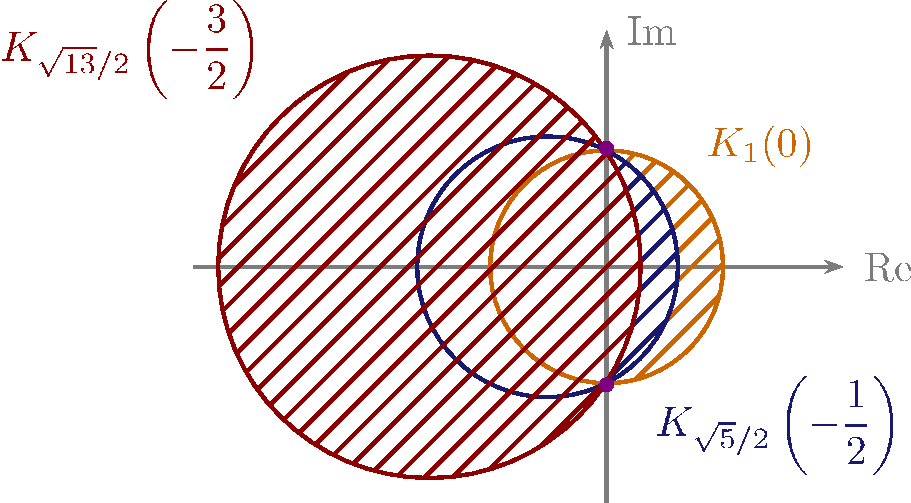
\includegraphics[scale=0.2]{images/ana3-tmp-35}
      \end{figure}
      %
      $\mathrm{Bild}(\Phi)$ ist kompakt ($\Phi$ ist stetig, $[0,1] \times [0,1]$ ist kompakt).
      %
      \begin{notice*}[Behauptung:]
        In $\mathrm{Bild}(\Phi)$ liegen nur endlich viele isolierte Singularitäten.
      \end{notice*}
      %
      \begin{notice*}[Annahme:]
        Es gibt mindestens abzählbar viele isolierte Singularitäten.
      \end{notice*}
      %
      \begin{align*}
        \overset{\mathrm{Bild}(\Phi) \text{ kompakt}}{\implies} \exists \text{ Häufungspunkt } z_0 \in \mathrm{Bild}(\Phi) .
      \end{align*}
      %
      Sei $(z_n)$ Folge in $S'$, $z_n \to z_0$, $z_n \neq z_0$.
      %
      \begin{align*} %FIXME: thm:4.8 referenziert fälschlicherweise ins Kapitel Mannigfaltigkeiten.
        \overset{\text{\ref{thm:4.8}}}{\implies}& \exists \, (\widetilde{z}_n) \in O : |\widetilde{z}_n - z_n| \leq \frac{1}{n} \land |f(\widetilde{z}_n)| \geq n \\
        \implies& \widetilde{z}_n \to z_0 \land |f(\widetilde{z}_n)| \to \infty \\
        \overset{\text{\ref{thm:4.8}}}{\implies}& \text{$f$ hat in $z_0$ einen Pol oder eine wesentliche Singularität} \\
        & \quad \lightning (z_n \to z_0 \text{ und } z_0 \text{ ist isolierte Singularität}).
      \end{align*}

      \item Für $z_0 \in S' \setminus \mathrm{Bild}(\Phi)$ gilt $\nu(\gamma,z_0) = 0$. Setze
      %
      \begin{align*}
        g(z) \coloneq \frac{1}{z - z_0}
      \end{align*}
      %
      holomorph in $\mathbb{C} \setminus \{z_0\}$.
      %
      \begin{gather*}
        \mathrm{Bild}(\Phi) \subseteq \mathbb{C} \setminus \{z_0\} \\
        \begin{aligned}
          \implies& \text{$\Phi$ ist eine Homotopie zwischen $\gamma$ und einer} \\
                  & \text{ konstanten Kurve in $\mathbb{C} \setminus \{z_0\}$.} \\ % FIXME: Mehrzeiliger Text im mathmode.
          \overset{\mathllap{\gamma \text{ nullhomotop}}\mspace{-50mu}}{\implies}& \int_\gamma \frac{1}{z-z_0} \, \mathrm{d}z = 0 \\
          \implies& \nu(\gamma,z_0) = 0 \\
          \implies& \sum\limits_{z \in S'} \ldots = \sum\limits_{z \in S''}  \ldots \overset{\text{\ref{itm:4.15 b)}}}{=} \text{endliche Summe}. \qquad S'' \coloneq S' \cap \mathrm{Bild}(\Phi)
        \end{aligned}
      \end{gather*}
    \end{enum-alph}

    \textbf{Schritt 2:} $S'' = \{ z_1,\ldots,z_n \}$, $H_j$ Hauptteil in $z_j$. Sei
    %
    \begin{align*}
      g(z) \coloneq f(z) - H_j(z)
    \end{align*}
    %
    holomorph in $O \setminus S$
    %
    \begin{align*}
      \implies& \text{$g$ hat in $\mathrm{Bild}(\Phi)$ nur hebbare Singularitäten.} \\
      \implies& \text{Es existiert eine holomorphe Fortsetzung $\widetilde{g}$ in einer} \\
              & \text{offenen Umgebung $U$ von $\mathrm{Bild}(\Phi)$.} \\ % FIXME: Mehrzeiliger Text im mathmode.
      \overset{\mathllap{\gamma \text{ nullhomotop in } U}\mspace{-50mu}}{\implies}& \int_{\gamma} g \, \mathrm{d}z = \int_\gamma \widetilde{g}(z) \, \mathrm{d}z = 0 \\
      \implies& \int_\gamma f(z) \, \mathrm{d}z = \underbrace{\int_\gamma g(z) \, \mathrm{d}z}_{=0} + \underbrace{\sum\limits_{j=1}^{n} \int_\gamma H_j(z) \, \mathrm{d}z}_{\overset{\text{\ref{thm:4.12}}}{=} 2 \pi \mathrm{i} \nu(\gamma,z_j) \mathrm{Res}(f,z_j)}
    \end{align*}
  \end{proof}
\end{theorem}

\begin{example} ~
  \begin{figure}[H]
    \centering
    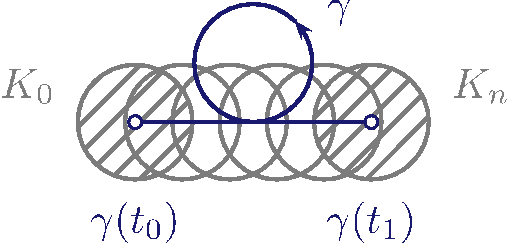
\includegraphics[scale=0.2]{images/ana3-tmp-36}
    \vspace*{-4em}
  \end{figure}
  %
  \begin{align*}
    \int_\gamma \frac{\mathrm{e}^{\mathrm{i} z}}{1 + z^2} \, \mathrm{d}z
  \end{align*}
  %
  $S = \{\pm \mathrm{i}\}$, $\nu(\gamma,-\mathrm{i}) = 0$. Berechne $\mathrm{Res}(f,\mathrm{i})$
  %
  \begin{align*}
    \frac{\mathrm{e}^{\mathrm{i} z}}{1 + z^2}
    &= \frac{\mathrm{e}^{\mathrm{i} z}}{2 \mathrm{i}} \left( \frac{1}{z - \mathrm{i}} - \frac{1}{z + \mathrm{i}} \right) \\
    &= \frac{\mathrm{e}^{\mathrm{i} z}}{2 \mathrm{i}} \frac{1}{z - \mathrm{i}} + \text{etwas Holomorphes für } z \neq -\mathrm{i}
  \end{align*}
  %
  $\dfrac{\mathrm{e}^{\mathrm{i} z}}{2 \mathrm{i}} \dfrac{1}{z - \mathrm{i}}$ hat in $z = \mathrm{i}$ einen Pol der Ordnung $1$.
  %
  \begin{gather*}
    a_{-1} = \frac{\mathrm{e}^{\mathrm{i} z}}{2 \mathrm{i}} \Big|_{z=\mathrm{i}} = \frac{\mathrm{e}^{-1}}{2 \mathrm{i}} \\
    \int_\gamma \frac{\mathrm{e}^{\mathrm{i} z}}{1 + z^2} \, \mathrm{d}z = 2 \pi \mathrm{i} \frac{\mathrm{e}^{-1}}{2 \mathrm{i}} 1 = \pi \mathrm{e}^{-1}
  \end{gather*}
\end{example}

% % % Vorlesung vom 26.11.2012

\begin{theorem}[Residuenberechnung] \label{thm:4.17}
  \begin{enum-arab}
    \item Falls $f$ in $z_0$ einen Pol der Ordnung $K$ hat:
    %
    \begin{align*}
      f(z) = \sum\limits_{n=-K}^{\infty} a_n (z-z_0)^n \; , \quad |z-z_0| < r, a_{-K} \neq 0 .
    \end{align*}
    %
    \begin{enum-alph}
      \item $K=1$:
      %
      \begin{align*}
        \boxed{a_{-1} = \lim\limits_{z \to z_0} (z-z_0) f(z)} = \lim\limits_{z \to z_0} \sum\limits_{n=-1}^{\infty} a_n (z-z_0)^{n+1}
      \end{align*}

      \item $K \geq 2$:
      %
      \begin{gather*}
        \frac{\mathrm{d}^{K-1}}{\mathrm{d}z^{K-1}} \left( (z-z_0)^K f(z) \right)
        = \sum\limits_{n=-1}^{\infty} (n+K) \ldots (n+2) a_n (z-z_0)^{n+1} \\
        \to (-1+K)(-1+K-1)\ldots(-1+2) a_{-1} \text{ für } z \to z_0 \\
        \implies \boxed{\mathrm{Res}(f,z_0) = a_{-1} = \lim\limits_{z \to z_0} \frac{1}{(K-1)!} \frac{\mathrm{d}^{K-1}}{\mathrm{d}z^{K-1}} \left( (z-z_0)^K f(z) \right)}
      \end{gather*}
    \end{enum-alph}

    \item Falls $f = g/h$, $g,h$ holomorph, $g(z_0) \neq 0$, $h(z_0) = 0$, $h'(z_0) \neq 0$, dann hat $f$ in $z_0$ einen Pol erster Ordnung. Sei
    %
    \begin{align*}
      \varphi(z) \coloneq
      \begin{dcases}
        \frac{h(z) - h(z_0)}{z - z_0} & z \neq z_0 \\
        h'(z_0) & z = z_0
      \end{dcases}
    \end{align*}
    %
    Dann ist $\varphi$ holomorph im Definitionsbereich von $h$.
    %
    \begin{align*}
      \implies&& f(z) &= (z-z_0) \varphi(z) \\
      \implies&& f(z) &= \frac{1}{z-z_0} \frac{g(z)}{\varphi(z)} \\
      \overset{K=1}{\implies}&& \mathrm{Res}(f,z_0) &= \lim\limits_{z \to z_0} (z-z_0) f(z) \\
      &&&= \frac{g(z_0)}{\varphi(z_0)} \\
      && \Aboxed{\mathrm{Res}(f,z_0) &= \frac{g(z_0)}{h'(z_0)}}
    \end{align*}
  \end{enum-arab}
\end{theorem}

\begin{example}
  \begin{enum-arab}
    \item $f(z) = \dfrac{\mathrm{e}^{\mathrm{i}z}}{1 + z^2}$, $z_0 = \mathrm{i}$.
    %
    \begin{align*}
      \overset{\text{\ref{thm:4.17}}}{\implies} \mathrm{Res}(f,\mathrm{i}) = \frac{\mathrm{e}^{\mathrm{i}z}}{2z} \Big|_{z=\mathrm{i}} = \frac{\mathrm{e}^{-1}}{2 \mathrm{i}} = -\frac{\mathrm{i}}{2 \mathrm{e}}
    \end{align*}

    \item Berechne
    %
    \begin{gather*}
      \int\limits_{-\infty}^{\infty} \frac{\cos x}{(1+x^2)^2} \mathrm{d}x \\
      \left| \frac{\cos x}{(1+x^2)^2} \right| \leq \frac{1}{1+x^2} \\
      \int\limits_{-\infty}^{\infty} \frac{1}{1+x^2} \mathrm{d}x < \infty \\
      \mathllap{\implies} \int\limits_{-\infty}^{\infty} \frac{\cos x}{(1+x^2)^2} \mathrm{d}x \text{ absolut konvergent}
    \end{gather*}
    %
    Betrachte $f(z) = \dfrac{\mathrm{e}^{\mathrm{i}z}}{(1+z^2)^2}$, denn $\Re f(x) = \dfrac{\cos x}{(1+x^2)^2}$ für $x \in \mathbb{R}$.
    %
    \begin{figure}[H]
      \centering
      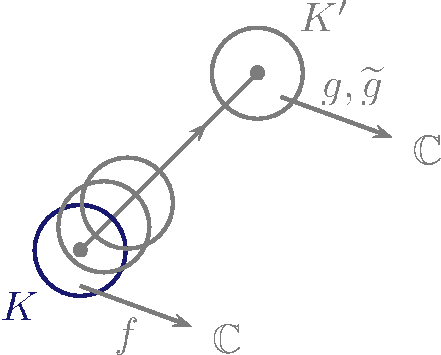
\includegraphics[scale=0.2]{images/ana3-tmp-37}
      \vspace*{-2em}
    \end{figure}
    %
    \begin{align*}
      \mathrm{Res}(f,\mathrm{i})
      &\overset{K=2}{\underset{\text{\ref{thm:4.17}}}{=}} \frac{1}{1!} \frac{\mathrm{d}}{\mathrm{d}z} \left( \frac{(z-\mathrm{i})^2 \mathrm{e}^{\mathrm{i}z}}{(1+z^2)^2} \right) \bigg|_{z = \mathrm{i}} \\
      &= \frac{\mathrm{d}}{\mathrm{d}z} \left( \frac{\mathrm{e}^{\mathrm{i}z}}{(z + \mathrm{i})^2} \right) \bigg|_{z = \mathrm{i}} \\
      &= \frac{\mathrm{i} \mathrm{e}^{\mathrm{i}z} (z+\mathrm{i})^2 - \mathrm{e}^{\mathrm{i}z} 2 (z+\mathrm{i})}{(z+\mathrm{i})^4}  \bigg|_{z = \mathrm{i}} \\
      &= \frac{\mathrm{i} \mathrm{e}^{-1} 2 \mathrm{i} - 2 \mathrm{e}^{-1}}{(2\mathrm{i})^3} = - \mathrm{i} \frac{\mathrm{e}^{-1}}{2}
    \end{align*}
    %
    Residuensatz
    %
    \begin{align*}
      \int_{\gamma_R} f(z) \, \mathrm{d}z = 2 \pi \mathrm{i} \left( - \mathrm{i} \frac{\mathrm{e}^{-1}}{2} \right) = \frac{\pi}{\mathrm{e}}
    \end{align*}
    %
    Für $|z| = R$, $\Im z \geq 0$:
    %
    \begin{gather*}
      |f(z)| = \left| \frac{\mathrm{e}^{\mathrm{i}z}}{(1+z^2)^2} \right| = \frac{\mathrm{e}^{-\Im z}}{|1+z^2|^2} \overset{|z^2+1|\geq||z^2|-1|}{\leq} \frac{1}{(|z|^2 - 1)^2} = \frac{1}{(R^2 - 1)^2} \\
      \begin{aligned}
        \implies \left| \int_{\substack{|z|=R}{\Im z > 0}} f(z) \, \mathrm{d}z \right|
        &\leq \max |f| \, L(\gamma) \\
        &\leq \frac{1}{(R^2 - 1)^2} \pi R \to 0 \; , \quad (R \to \infty)
      \end{aligned} \\
      \implies \frac{\pi}{\mathrm{e}} = \int_{\gamma_R} f(z) \, \mathrm{d}z = \lim\limits_{R \to \infty} \int_{\gamma_R} f(z) \, \mathrm{d}z = \int\limits_{-\infty}^{\infty} \frac{\cos x + \mathrm{i} \sin x}{(1+x^2)^2} \\
      \implies \int\limits_{-\infty}^{\infty} \frac{\cos x}{(1+x^2)^2} \mathrm{d}x = \frac{\pi}{\mathrm{e}} .
    \end{gather*}
  \end{enum-arab}
\end{example}

\begin{theorem}[Definition] \label{thm:4.19}
  Sei $G \subseteq \mathbb{C}$ ein Gebiet. Ein geschlossener Weg $\gamma$ in $\mathbb{C}$ \acct{berandet} $G$, falls
  %
  \begin{align*}
    \nu(\gamma,z) =
    \begin{dcases}
      1 & z \in G \\
      0 & z \in \mathbb{C}\setminus \overline{G}
    \end{dcases}
  \end{align*}
\end{theorem}

\begin{example*}
  \begin{enum-arab}
    \item $G = K_1(0)$, $\gamma_N(t) = \mathrm{e}^{2 \pi \mathrm{i} t N}$, $0 \leq t \leq 1$.
    %
    \begin{figure}[H]
      \centering
      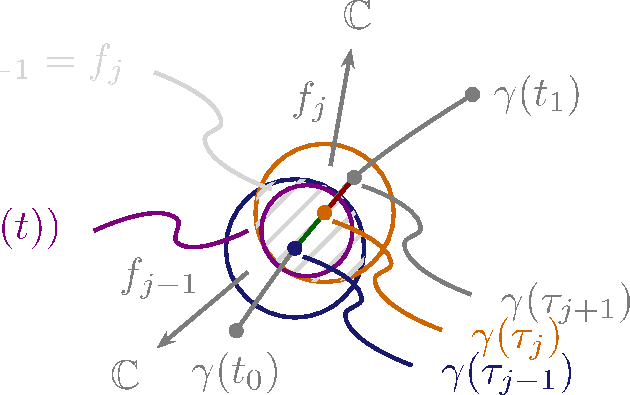
\includegraphics[scale=0.2]{images/ana3-tmp-38}
      \vspace*{-2em}
    \end{figure}
    %
    $\nu(\gamma,z_1) = 1$, falls $|z_1| < 1$ und $\nu(\gamma,z_2) = 0$, falls $|z_2| > 1$.

    $\gamma_1$ berandet $G$, $\gamma_N$ berandet $G$ nicht.

    \item $G = K_{1,2}(0)$
    %
    \begin{figure}[H]
      \centering
      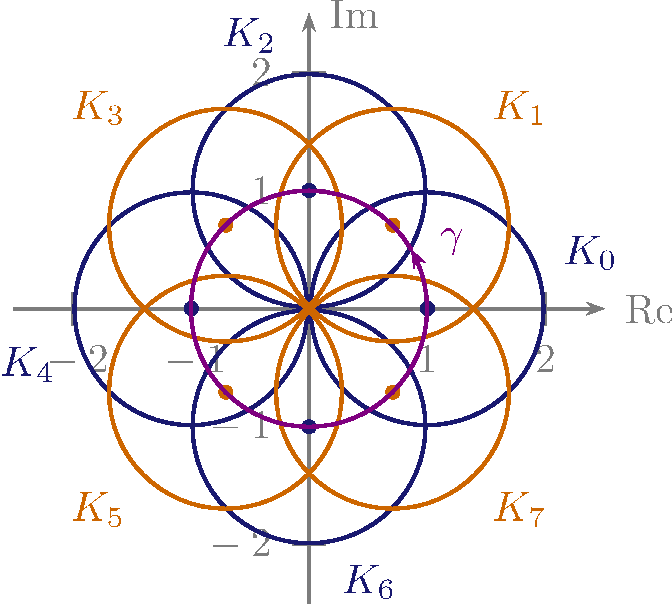
\includegraphics[scale=0.2]{images/ana3-tmp-39}
      \vspace*{-2em}
    \end{figure}
    %
    Der Rand besteht aus zwei disjunkten Wegen (Zykel). Deshalb greift hier unsere Definition nicht.
  \end{enum-arab}
\end{example*}

\begin{theorem}[Definition] \label{thm:4.20}
  Sei $O \subseteq \mathbb{C}$ offen, $f$ holomorph in $O \setminus S$ (insbesondere $O \setminus S$ offen) und
  %
  \begin{align*}
    \forall \, z \in S : f \text{ hat einen Pol in } z.
  \end{align*}
  %
  Dann heißt $f$ \acct{meromorph} in $O$.
  %
  \begin{figure}[H]
    \centering
    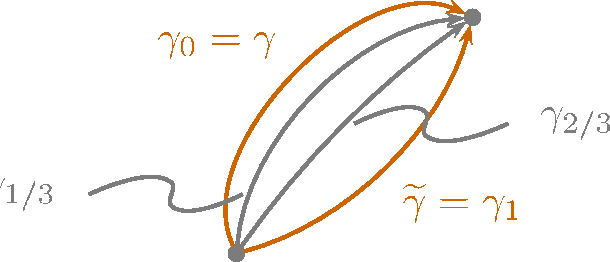
\includegraphics[scale=0.2]{images/ana3-tmp-40}
  \end{figure}
\end{theorem}

% % % Vorlesung vom 29.11.2012

\begin{theorem}[Null- und Polstellen zählendes Integral] \label{thm:4.21}
  Sei $f$ meromorph in $O$, $G$ ein Gebiet, $\overline{G} \subset O$ und $\gamma$ ein Weg in $O$ der $G$ berandet und keine Null- oder Polstelle trifft. Dann gilt
  %
  \begin{align*}
    \frac{1}{2\pi \mathrm{i}} \int_\gamma \frac{f'(z)}{f(z)} \, \mathrm{d}x = N_G - P_G
  \end{align*}
  %
  wobei $N_G$ die Anzahl der Nullstellen in $G$ und $P_G$ die Anzahl der Pole in $G$ bezeichnet, jeweils mit Ordnung gezählt.

  \begin{proof}
    Sei $S \coloneq \{ z \in O : f(z) = 0 \lor f\text{ hat Pol in }z \}$.
    Dann besteht $S$ nur aus isolierten Punkten (Nullstellen nach \ref{thm:3.8}, Polstellen nach Definition).
    %
    \begin{align*}
      g \coloneq \frac{f'}{f} \quad \text{ist holomorph in $O \setminus S$}
    \end{align*}
    %
    Nach dem Residuensatz ist
    %
    \begin{align*}
      \int_\gamma g(z) \, \mathrm dz = \sum_{z \in S} 2 \pi \mathrm{i} \mathrm{Res}(g,z) \underbrace{\nu(\gamma,z)}_{= \begin{cases} 1 & z \in G \\ 0 & z \in O \setminus G \end{cases}} = \sum_{z \in S \cap G} 2 \pi \mathrm{i} \mathrm{Res}(g,z)
    \end{align*}
    %
    Betrachte einen einzelnen Summanden, bzw. ein $z_0 \in S \cap G$ und schreibe:
    %
    \begin{align*}
      f(z) = (z-z_0)^k \widetilde{f}(z) \qquad \widetilde{f}(z_0) \neq 0
    \end{align*}
    %
    mit holomorphem $\widetilde{f}$.
    Für $k\ge 1$ ist $k$ die Ordnung der Nullstelle und für $k \le -1$ ist $-k$ die Ordnung des Pols.
    %
    \begin{align*}
      f'(z) &= k (z-z_0)^{k-1} \widetilde{f}(z) + (z-z_0)^k \widetilde{f}'(z) \\
      g(z) &= \frac{f'(z)}{f(z)} = \frac{k}{(z-z_0)} + \underbrace{\frac{\widetilde{f}'(z)}{\widetilde{f}(z)}}_{\text{holomorph bei $z_0$}}
    \end{align*}
    %
    Damit ist
    %
    \begin{align*}
      \mathrm{Res}(g,z_0) = \lim\limits_{z \to z_0} (z-z_0) g(z) = k
    \end{align*}
    %
    Betrachtet man nun wieder die Summe, so ergibt sich sofort die Behauptung.
  \end{proof}
\end{theorem}

\begin{example}
  \begin{align*}
    f(z) = \frac{(z-2)(z-3)}{(z-1)^2}
  \end{align*}
  %
  ist meromorph in $\mathbb C$.
  %
  \begin{figure}[H]
    \centering
    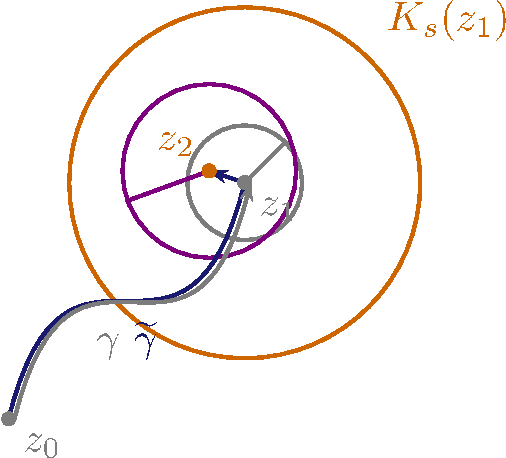
\includegraphics[scale=0.2]{images/ana3-tmp-41}
    \vspace*{-3em}
  \end{figure}
  %
  \begin{align*}
    \frac{1}{2\pi \mathrm{i}} \int_{\gamma_j} \frac{f'(z)}{f(z)} \, \mathrm dz
    =
    \begin{cases}
      -2 & j=1 \\
      1 & j=2,3 \\
      0 & j=4
    \end{cases}
  \end{align*}
\end{example}

\begin{notice}[Folgerung (Null- und Polstellen zählendes Integral 2)] \label{thm:4.22}
  Seien die Voraussetzungen wie in \ref{thm:4.21}.
  Dann gilt
  %
  \begin{align*}
    N_G - P_G = \nu(f \circ \gamma, 0)
  \end{align*}

  \begin{proof}
    Sei $\gamma : [a,b] \to \mathbb{C}$, dann gilt nach \ref{thm:4.41}: % FIXME: 4.41 existiert nicht.
    %
    \begin{align*}
      N_G - P_G &= \frac{1}{2 \pi \mathrm{i}} \int_\gamma \frac{f'(z)}{f(z)} \, \mathrm{d}z \\
      &= \frac{1}{2\pi \mathrm{i}} \int_a^b \frac{1}{\underbrace{f(\gamma(t))}_{= \frac{1}{f \circ \gamma}}} \underbrace{f'(\gamma(t)) \gamma'(t)}_{=(f \circ \gamma)'} \mathrm{d}t
    \intertext{(wobei das Integral evtl. eine Summe über Teilintervalle ist)}
      &= \frac{1}{2\pi \mathrm{i}} \int_{f \circ \gamma} \frac{1}{z} \, \mathrm{d}z \\
      &= \nu(f \circ \gamma, 0)
    \end{align*}
  \end{proof}
\end{notice}

\begin{theorem}[Satz von Rouch\'{e}] \label{thm:4.23}
  Seien $f$, $g$ holomorph in $\mathbb{O}$, $G \subseteq O$ berandet vom Weg $\gamma$ in $O$. Gilt
  %
  \begin{align*}
    |g(z)| < |f(z)| \text{ für } z \in \mathrm{Bild}(\gamma)
  \end{align*}
  %
  dann haben $f$ und $f+g$ gleich viele Nullstellen in $G$ (die Nullstellen mit Ordnung gezählt).

  \begin{proof}
    Mit \ref{thm:4.22}
    %
    \begin{align*}
      N_G(f) &= \nu(f \circ \gamma, 0) \\
      N_G(f+g) &= \nu((f+g) \circ \gamma, 0)
    \end{align*}
    %
    Zeige, dass $f \circ g \sim (f+g) \circ \gamma$ in $\mathbb{C} \setminus \{O\}$.

    $\gamma$ muss eventuell umparametrisiert werden, damit $\gamma \in C^1$.
    %
    \begin{align*}
      \Phi(t,s) \coloneq (f \circ \gamma) (t) + s (g \circ \gamma)(t)
    \end{align*}
    %
    dann
    %
    \begin{align*}
      \left.
      \begin{aligned}
        \Phi &\in C^1([0,1] \times [0,1] \to \mathbb{C}) \\
        \Phi(t,0) &= (f \circ \gamma)(t) \\
        \Phi(t,1) &= ((f+g) \circ \gamma)(t) \\
        \Phi &\in \mathrm{Bild}(\Phi) \qquad {\color{DarkRed} (*)}
      \end{aligned}
      \right\} \implies \text{ fertig}
    \end{align*}
    %
    Zu ${\color{DarkRed} (*)}$:
    %
    \begin{align*}
      \left| (f \circ \gamma) (t) + s (g \circ \gamma) (t) \right|
      &= \left| f(\gamma(t)) + s \, g(\gamma(t)) \right| \\
      &\geq \left| f(\gamma(t)) \right| - s \left| g(\gamma(t)) \right|
    \intertext{da $0 \leq s \leq 1$}
      &\geq \left| f(\gamma(t)) \right| - \left| g(\gamma(t)) \right| \\
      &\geq 0 \text{ nach Vereinbarung.}
    \end{align*}
  \end{proof}
\end{theorem}

\begin{notice*}[Folgerung]
  Sei
  %
  \begin{align*}
    p(z) = z^n + \sum\limits_{k=0}^{n-1} a_k \, z^k .
  \end{align*}
  %
  Dann hat $p$ in $\overline{K_R(0)}$ mit
  %
  \begin{align*}
    R \coloneq \max \left\{ \sum\limits_{k=0}^{n-1} |a_k| , 1 \right\}
  \end{align*}
  %
  genau $n$ Nullstellen (mit Vielfachheit gezählt). Dies sind alle Nullstellen von $p$.

  \begin{proof}
    Seien
    %
    \begin{align*}
      f(z) = z^n \qquad g(z) &= \sum\limits_{k=0}^{n-1} a_k \, z^k \\
      \implies \quad f + g &= p
    \end{align*}
    %
    $f$ hat die $n$-fache Nullstelle $z_0 = 0$ und sonst keine in jeder Kreisscheibe $G = K_r(0)$ mit $r > 0$. Sei nun $r > R$. Zeige
    %
    \begin{align*}
      |g(z)| < |f(z)| \; , \quad \text{ für } |z| = r.
    \end{align*}
    %
    Dann folgt aus Rouch\'{e} (\ref{thm:4.23}) die gesamte Behauptung.
    %
    \begin{align*}
      P_N(f+g) &= P_N(f) = n \text{ in jedem } K_r(0) \text{ mit } r > R \\
      |g(z)| &\overset{|z| = r}{\leq} \sum\limits_{k=0}^{n-1} |a_k| \, r^k
    \intertext{aus $r > R \geq 1$ folgt $r^k \leq r^{n-1}$}
      &\leq \underbrace{\sum\limits_{k=0}^{n-1} |a_k|}_{\leq R < r} \, r^{n-1} \\
      &< r^n = |f(z)|
    \end{align*}
  \end{proof}
\end{notice*}

%
% Henri Menke, 2012 Universität Stuttgart.
%
% Dieses Werk ist unter einer Creative Commons Lizenz vom Typ
% Namensnennung - Nicht-kommerziell - Weitergabe unter gleichen Bedingungen 3.0 Deutschland
% zugänglich. Um eine Kopie dieser Lizenz einzusehen, konsultieren Sie
% http://creativecommons.org/licenses/by-nc-sa/3.0/de/ oder wenden Sie sich
% brieflich an Creative Commons, 444 Castro Street, Suite 900, Mountain View,
% California, 94041, USA.

\section{Analytische Fortsetzung}
\addtocounter{thmn}{1}
\setcounter{theorem}{0}

% % % Vorlesung vom 29.11.2012

\begin{example}
  Betrachte
  %
  \begin{align*}
    f(z) = \sum\limits_{n=0}^{\infty} (-z^2)^n \quad \text{ für } |z| < 1
  \end{align*}
  %
  und $f(z) = \dfrac{1}{1 + z^2}$ (geometrische Reihe). Sei
  %
  \begin{align*}
    g(z) \coloneq \frac{1}{1 + z^2} \quad \text{ für } z \neq \pm \mathrm{i}
  \end{align*}
  %
  \begin{figure}[H]
    \centering
    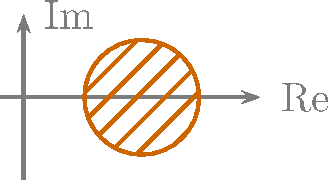
\includegraphics[scale=0.2]{images/ana3-tmp-42}
  \end{figure}
  %
  Entwickle $f$ um $z = -1/2$ in eine Potenzreihe
  %
  \begin{align*}
    f_1(z) = \sum\limits_{n=0}^{\infty} a_n (z-z_1)^n
  \end{align*}
  %
  Wir wissen: $f = g$ in $K_1(0)$, also ist $f_1$ gleichzeitig Entwicklung von $g$.

  $\implies$ $f_1$ hat den Konvergenzradius $r_1 = \dfrac{\sqrt{5}}{2}$.

  Entwickle $f_1$ um $z_2 = -\dfrac{3}{2}$:
  %
  \begin{align*}
    f_2(z) = \sum\limits_{n=0}^{\infty} b_n (z-z_2)^n \quad \text{ in } K_{r_2}(z_2)
  \end{align*}
  %
  mit $r_2 = \dfrac{\sqrt{13}}{2}$ (da $f_2$ Entwicklung von $g$ ist). Wir haben $f$, das nur auf $K_1(0)$ definiert ist holomorph auf $K_1(0) \cup K_{\sqrt{5}/{2}}(-1/2) \cup K_{\sqrt{13}/2}(-3/2)$ fortgesetzt.
\end{example}

\begin{theorem}[Definition]
  Ein Tupel $\mathcal{K} = (K_0,\ldots,K_n)$ offener Kreisscheiben $K_j = K_{r_j}(z_j)$ heißt \acct{Kreiskette}, falls
  %
  \begin{align*}
    z_j \in K_{j-1} \lor z_{j-1} \in K_{j} \; , \quad j = 1,\ldots,n
  \end{align*}
  %
  Sind $f_j : K_j \to \mathbb{C}$ holomorph mit
  %
  \begin{align*}
    f_j \Big|_{K_j \cap K_{j-1}} = f_{j-1} \Big|_{K_j \cap K_{j-1}} \; , \quad j = 1,\ldots,n
  \end{align*}
  %
  so heißt $f_0$ \acct{analytisch fortsetzbar} längs $\mathcal{K}$, $f_n$ heißt \acct{analytische Fortsetzung} von $f_0$ längs $\mathcal{K}$.
\end{theorem}

\begin{notice}
  \begin{enum-arab}
    \item  Nach dem Identitätssatz ist $f_1$ und dann auch $f_2,\ldots,f_n$ eindeutig.

    \item Sind $(K_0,\ldots,K_n)$, $(\widetilde{K}_0,\ldots,\widetilde{K}_m)$ Kreisketten mit $\widetilde{K}_0 = K_0$ und $\widetilde{K}_m = K_n$, gilt dann $\widetilde{f}_m = f_n$? (Im Allgemeinen nein)
  \end{enum-arab}
\end{notice}

\begin{theorem}[Defintion]
  Sei $\gamma \in C([t_0,t_1] \to \mathbb{C})$. Eine Kreiskette $\mathcal{K} = (K_0,\ldots,K_n)$ verläuft \acct{längs} $\gamma$, falls es eine Unterteilung $t_0 = \tau_0 < \tau_1 < \ldots < \tau_n < t_1$ gibt, sodass
  %
  \begin{gather*}
    \gamma(\tau_j) \text{ Mittelpunkt von } K_j \; , \quad j = 0,\ldots,n \\
    \gamma([\tau_{j-1},\tau_{j}]) \subseteq K_{j-1} \cap K_j \; , \quad j = 1,\ldots,n
  \end{gather*}
  %
  Die zweite Bedingung verhindert, dass $\gamma$ wie im Bild aus der Kreiskette hinausläuft.
  %
  \begin{figure}[H]
    \centering
    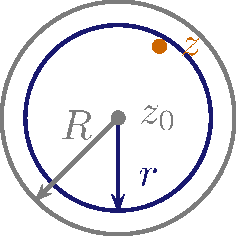
\includegraphics[scale=0.2]{images/ana3-tmp-43}
  \end{figure}
\end{theorem}

\begin{example}
  Sei $N \in \mathbb{N}$, $N \geq 2$, $\gamma(t) = \mathrm{e}^{2 \pi \mathrm{i} t}$, $0 \leq t \leq N$. Sei
  %
  \begin{align*}
    \tau_j &\coloneq \frac{j}{8} \; , \quad j = 0,\ldots,8N \\
    K_j &\coloneq K_1(\gamma(\tau_j)) \; , \quad j = 0,\ldots,8N
  \end{align*}
  %
  Dann verläuft $\mathcal{K} = (K_0,\ldots,K_{8N})$ längs $\gamma$.
\end{example}

% % % Vorlesung vom 03.12.2012

\begin{figure}[H]
  \centering
  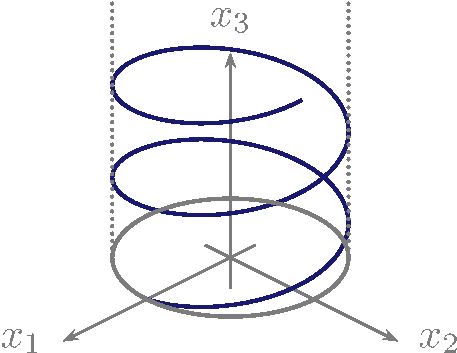
\includegraphics[scale=0.2]{images/ana3-tmp-44}
\end{figure}

\begin{theorem}[Satz] \label{thm:5.6}
  Seien $\gamma \in C([t_0,t_1] \to \mathbb{C})$, $K,K'$ offene Kreisscheiben um $\gamma(t_0)$ bzw. $\gamma(t_1)$, $f$ holomorph in $K$ und $g,\widetilde{g}$ holomoprh in $K'$ und $g,\widetilde{g}$ seien aus $f$ durch analytische Fortsetzung längs Kreisketten entstanden, die längs $\gamma$ verlaufen. Dann gilt
  %
  \begin{align*}
    g = \widetilde{g}
  \end{align*}

  \begin{proof}
    \begin{enum-arab}
      \item Vorüberlegung

      \begin{figure}[H]
        \centering
        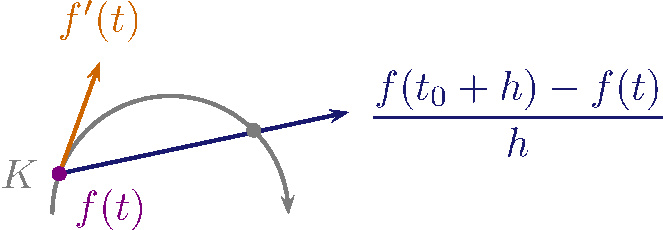
\includegraphics[scale=0.2]{images/ana3-tmp-45}
      \end{figure}

      Sei $t_0 = \tau_0 < \tau_1 < \ldots < \tau_n = t_1$ die Unterteilung von $[t_0,t_1]$ mit Kreiskette $K = K_0,K_1,\ldots,K_n=K'$ und holomorphe Funktionen $f_j : K_j \to \mathbb{C}$, die $f$ zu $g$ fortsetzen. Für $t \in [\tau_{j-1},\tau_j]$ sei
      %
      \begin{align*}
        P_t(z) \coloneq \sum\limits_{n=0}^{\infty} a_n(t) (z-\gamma(t))^n \; , \quad z \in K_{r(t)}(\gamma(t))
      \end{align*}
      %
      die Potenzreihenentwicklung von $f_{j-1}$ um $\gamma(t)$. Beachte: $P_t$ ist auch die Potenzreihe von $f_j$ um $\gamma(t)$, da $f_j = f_{j-1}$ in $K_j \cap K_{j-1}$. Also in $P_t$ Potenzreihenentwicklung von $f_j$ um $\gamma(t)$ sogar für $t \in [\tau_{j-1},\tau_{j+1}]$. Da $\gamma$ stetig: Für festes $t \in [t_0,t_1]$
      %
      \begin{align*}
        \exists \, \delta > 0 : |\gamma(t') - \gamma(t)| < r(t) \text{ für } |t'-t| < \delta \text{, } t_0 \leq t' \leq t_1
      \end{align*}
      %
      Wähle $\delta$ so klein, dass $t,t'$ im selben Intervall $[\tau_{j-1},\tau_{j+1}]$ liegen.

      $\implies$ Für $|t'-t| < \delta$ erhält man $P_{t'}$ durch Entwicklung von $P_t$ um $\gamma(t')$, da um $\gamma(t') : P_t = f_j$

      Das nennt man die \acct[0]{lokale Verträglichkeit der Familie $(P_t)_{t_0 \leq t \leq t_1}$}.

      Dasselbe für $\widetilde{g}$: Unterteilung $t_0 = \sigma_0 < \sigma_1 < \ldots < \sigma_m = t_1$, $\widetilde{P}_t$ Entwicklung von $\widetilde{f}_j$ um $\gamma(t)$.

      \item Eigentlicher Beweis
      %
      \begin{align*}
        M \coloneq \{t \in [t_0,t_1] : P_t = \widetilde{P}_t \}
      \end{align*}
      %
      Zeige: $M = [t_0,t_1] \implies g = P_{t_1} = \widetilde{P}_{t_1} = \widetilde{g}$.
      %
      \begin{enum-arab}
        \item \label{itm:5.6 a)} $M \neq \emptyset$: Wegen $f_0 = f = \widetilde{f}_0$ gilt $[t_0,t_0 + \delta] \subseteq M$, $\delta$ so gewählt, dass $\gamma(t) \in K = K_0 = \widetilde{K}_0$ für $t_0 \leq t \leq t_0 + \delta$.

        \item \label{itm:5.6 b)} $M$ ist relativ offen\footnote{relativ offen: Ich kann $M$ bekommen durch den Schnitt einer offenen Menge mit $[t_0,t_1]$}: Sei $s \in M$, $\delta > 0$ so klein, dass \[|\gamma(t) - \gamma(s)| < \min\{r(s),\widetilde{r}(s)\} \text{ für } s - \delta < t < s + \delta\] (Stetigkeit von $\gamma$). Aus der lokalen Verträglichkeit folgt: $P_t$ entsteht aus Entwicklung von $P_s$ um $\gamma(t)$ genauso $\widetilde{P}_t$ aus $\widetilde{P}_s$.
        %
        \begin{align*}
          P_s \overset{s \in M}{=} \widetilde{P}_s \implies P_t = \widetilde{P}_t \text{ für } s - \delta < t < s + \delta
        \end{align*}

        \item \label{itm:5.6 c)} $M$ ist abgeschlossen: Sei $(s_n)$ in $M$, $s_n \to s$, $s_n \neq s$. Dann gilt $\gamma(s_n) \to \gamma(s)$ und entweder $\gamma(s_n) = \gamma(s)$ für ein $n$ $\implies$ $s \in M$, da $P_s = P_{s_n}$ oder $\gamma(s_n) \neq \gamma(s)$ für $n \in \mathbb{N}$: Für $n > N_\delta$:
        \begin{align*}
          P_s(\gamma(s_n)) = P_{s_n}(\gamma(s_n)) = \widetilde{P}_{s_n}(\gamma(s_n)) = \widetilde{P}_s(\gamma(s_n))
          \overset{\text{Identitätssatz}}{\implies} \widetilde{P}_s = P_s .
        \end{align*}
      \end{enum-arab}
      %
      \ref{itm:5.6 a)}, \ref{itm:5.6 b)} und \ref{itm:5.6 c)} $\implies$ $M = [t_0,t_1]$.
    \end{enum-arab}
  \end{proof}
\end{theorem}

\begin{theorem}[Definition]
  Sei $\gamma \in C([t_0,t_1] \to \mathbb{C})$, $K,K'$ offene Kreisscheiben um $\gamma(t_0)$ bzw. $\gamma(t_1)$. $f$ holomorph in $K$, $g$ holomorph in $K'$. Dann heißt $g$ \acct{analytische Fortsetzung} von $f$ längs $\gamma$, falls es eine längs $\gamma$ verlaufende Kreiskette $\mathcal{K}$ gibt, sodass $g$ analytische Fortsetzung von $f$ längs $\mathcal{K}$ ist.
\end{theorem}

\begin{example} Seien
  $N \in \mathbb{N}$, $N \geq 2$, $f(z) = |z|^{1/N} \mathrm{e}^{\mathrm{i}\frac{1}{N}\arg z}$
  %
  \begin{align*}
    \gamma(t) = \mathrm{e}^{2 \pi \mathrm{i} t} \; , \quad 0 \leq t \leq N
  \end{align*}
  %
  $\tau_j = \dfrac{j}{8N}$, $K_j = K_1(\gamma(\tau_j))$, $j = 0,\ldots,8N$.
  %
  \begin{figure}[H]
    \centering
    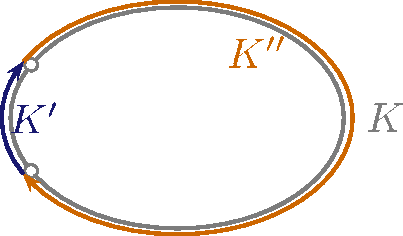
\includegraphics[scale=0.2]{images/ana3-tmp-46}
  \end{figure}
  %
  Setze $f$ längs $K_0,K_1,\ldots,K_{8N}$ fort
  %
  \begin{align*}
    f_0 = f \Big|_{K_0} \text{ für } j = 1,2
  \end{align*}
  %
  Wie sieht $f_3$ aus?
  %
  \begin{align*}
    \arg_\pi (z) \coloneq
    \begin{dcases}
      \arg(z) & \Im z > 0 \\
      \pi & z \in ]-\infty,0[ \\
      \arg(z+2\pi) & \Im z < 0
    \end{dcases}
  \end{align*}
  %
  Setze $g_1(z) \coloneq |z|^{1/N} \mathrm{e}^{\mathrm{i}\frac{1}{N}\arg_\pi z}$
  %
  \begin{align*}
    \implies&
    \begin{cases}
      g_1 \text{ holomorph in } \mathbb{C} \setminus [0,\infty[ \\
      g_1 \Big|_{\{z: \Im z > 0\}} = f \Big|_{\{z: \Im z > 0\}}
    \end{cases} \\
    \implies&
    f_j = g_1 \Big|_{K_j} \; , \quad j = 3,4,5,6
  \end{align*}
  %
  Setze $g_2(z) \coloneq |z|^{1/N} \mathrm{e}^{\mathrm{i}\frac{1}{N}\arg_\pi (z+2\pi)}$
  %
  \begin{align*}
    \implies&
    \begin{cases}
      g_2 \text{ holomorph in } \mathbb{C} \setminus ]-\infty,0] \\
      g_2 \Big|_{\{z: \Im z < 0\}} = g_1 \Big|_{\{z: \Im z < 0\}}
    \end{cases} \\
    \implies&
    f_j = g_2 \Big|_{K_j} \; , \quad j = 7,8,9,10
  \end{align*}
  %
  Beachte: $K_8 = K_0$, aber $f_8 = \mathrm{e}^{\mathrm{i}\frac{2 \pi}{N}} f_0 \neq f_0$.
  %
  \begin{align*}
    f_{16} &= \mathrm{e}^{\mathrm{i} \, 2 \frac{2 \pi}{N}} f_0 \neq f_0 \\
    &\vdots \\
    f_{8N} &= \mathrm{e}^{\mathrm{i} \, N \frac{2 \pi}{N}} f_0 = f_0
  \end{align*}
  %
  Nach der $N$-ten Umkreisung der $0$ landen wir wieder bei der ursprünglichen Funktion.
\end{example}

\begin{theorem}[Umparametrisierung]
  Sei $\gamma \in C([t_0,t_1] \to \mathbb{C})$, $f_1$ analytische Fortsetzung von $f$ längs $\gamma$, $\varphi : [s_0,s_1] \to [t_0,t_1]$ stetig, streng monoton wachsend, $\varphi(s_0) = t_0$, $\varphi(s_1) = t_1$. Damit ist $f_1$ auch analytische Fortsetzung von $f$ längs $\gamma \circ \varphi$. Insbesondere kann immer $s_0 = 0$, $s_1 = 1$ gewählt werden.

  \begin{proof}
    Verwende dieselbe Kreiskette, als Unterteilung von $[s_0,s_1] : s_j = \varphi^{-1}(\tau_j)$.
  \end{proof}
\end{theorem}

\begin{theorem}[Monodromiesatz] \label{thm:5.10}
  Seien $\gamma, \widetilde{\gamma} \in C([0,1] \to \mathbb{C})$ mit $\gamma(0) = \widetilde{\gamma}(0)$, $\gamma(1) = \widetilde{\gamma}(1)$. Weiter sei $\Phi \in C([0,1] \times [0,1] \to \mathbb{C})$ eine Homotopie zwischen $\gamma,\widetilde{\gamma}$, das heißt
  %
  \begin{gather*}
    \Phi(\cdot,0) = \gamma \qquad \Phi(\cdot,1) = \widetilde{\gamma} \\
    \Phi(0,s) = \gamma(0) \qquad \Phi(1,s) = \gamma(1) \; , \quad 0 \leq s \leq 1
  \end{gather*}
  %
  Ist $f_0$ holomorph in einer Kreisscheibe $K_r(\gamma(0))$ und lässt sich $f_0$ längs jedes Weges $\gamma_s \coloneq \Phi(\cdot,s)$ analytisch fortsetzen, dann stimmen die analytischen Fortsetzungen von $f_0$ längs $\gamma$ und $\widetilde{\gamma}$ überein.

  \begin{figure}[H]
    \centering
    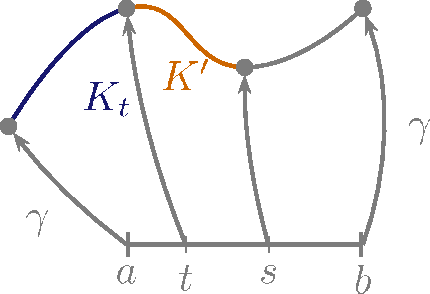
\includegraphics[scale=0.2]{images/ana3-tmp-47}
  \end{figure}
  %
  Der Beweis verläuft ähnlich wie in \ref{thm:5.6}.
\end{theorem}

\begin{theorem}[Definition]
  Ein Gebiet $G \subseteq \mathbb{C}$ heißt \acct{einfach zusammenhängend}, wenn jede geschlossene stetige Kurve $\gamma$ in $G$ nullhomotop ist, das heißt es existiert eine Homotopie $\Phi \in C([0,1] \times [0,1] \to G)$ zwischen $\gamma$ und einer konstanten Kurve.

  Oder äquivalent: Zu je zwei Kurven $\gamma_1,\gamma_2 \in C([0,1] \to G)$ mit $\gamma_1(0) = \gamma_2(0)$ und $\gamma_1(1) = \gamma_2(1)$ existiert eine Homotopie $\Phi \in C([0,1] \times [0,1] \to G)$.
\end{theorem}

\begin{example*}
  \begin{align*}
    \mathbb{C} \setminus [0,\infty[ \quad &\text{Gebiet, einfach zusammenhängend}\\
    \mathbb{C} \setminus \{0\} \quad  & \text{Gebiet, nicht einfach zusammenhängend} \\
    & \text{(Der Kreis um die $0$ ist nicht nullhomotop)}
  \end{align*}
\end{example*}

% % % Vorlesung vom 06.12.2012

\begin{notice}[Folgerung]
  $G \subseteq \mathbb{C}$ einfach zusammenhängendes Gebiet, $f_0$ holomorph in $K_r(z_0) \subseteq G$. Lässt sich $f_0$ längs jeder stetigen Kurve $\gamma$ mit Anfangspunkt $z_0$ analytisch fortsetzen, dann gibt es genau eine holomorphe Funktion
  %
  \begin{align*}
    f : G \to \mathbb{C} \quad \text{mit} \quad f \Big|_{K_r(z_0)} = f_0
  \end{align*}
  %
  \begin{proof}
    \begin{enum-arab}
      \item Definiere $f : G \to \mathbb{C}$. Sei $z_1 \in G$. Da $G$ ein Gebiet ist folgt: Es existiert eine stetige Kurve $\gamma$ von $z_0$ nach $z_1$. Setze $f_0$ längs $\gamma$ fort zu $f_1 : K_s(z_1) \to \mathbb{C}$ ($f_1$ ist holomorph). Setze $f(z_1) \coloneq f_1(z_1)$. $f$ ist sinnvoll definiert: Ist $\widetilde{\gamma}$ eine andere stetige Kurve von $z_0$ nach $z_1$. Da $G$ einfach zusammenhängend ist folgt $\gamma \sim \widetilde{\gamma}$.

      Monodromiesatz \ref{thm:5.10}: Fortsetzung längs $\widetilde{\gamma}$ liefert dieselbe Funktion $f_1$.

      \item Zeige: $f$ ist holomorph. Sei $z_1 \in G$ fest, $f_1$ wie oben. Zeige \[ f \Big|_{K_{s/3}}(z_1). \] Dann ist $f$ holomorph in $K_{s/3}(z_1)$. Da $z_1 \in G$ holomorph ist, ist $f$ holomorph in $G$.

      \begin{figure}[H]
        \centering
        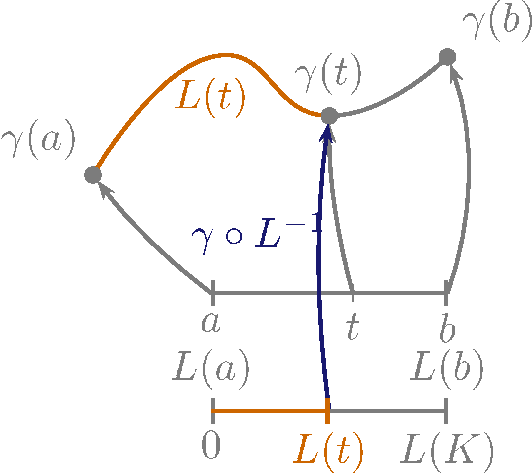
\includegraphics[scale=0.2]{images/ana3-tmp-48}
      \end{figure}

      Sei $z_2 \in K_{s/3}(z_1)$. Bilde $\widetilde{\gamma}$ aus $\gamma$ durch Anhängen der Strecke $z_1 z_2$. Ergänze dei Kreiskette $\mathcal{K}$ längs $\gamma$, die zur Fortsetzung längs $\gamma$ verwendet wurde, durch $K_{s/2}(z_2)$ zur Kreiskette $\widetilde{\mathcal{K}}$ längs $\widetilde{\gamma}$. $f(z_2)$ wird definiert durch analytische Fortsetzung von $f_0$ längs $\widetilde{\gamma}$. Dies liefert $f_2 : K_{s/2}(z_2) \to \mathbb{C}$. Wegen \[ f_2 = f_1 \text{ in } K_{s/2}(z_2) \cap K_s(z_1) \] folgt $f(z_2) \coloneq f_2(z_2) = f_1(z_2)$.

      \item Zeige: $f$ ist eindeutig. Ist $\mathcal{K} = (K_1,\ldots,K_n)$ Kreiskette längs $\gamma$, so ist $f \Big|_{K_j}$ eine analytische Fortsetzung längs $\gamma$. Aus Satz \ref{thm:5.6} folgt: Jede andere Fortsetzung längs $\gamma$ liefert dieselbe analytische Fortsetzung.
    \end{enum-arab}
  \end{proof}
\end{notice}

\begin{example}
  \begin{align*}
    f_0(z) = |z|^{1/N} \mathrm{e}^{\mathrm{i}\frac{1}{N}\arg z} \quad \text{in } K_1(2)
  \end{align*}
  %
  \begin{figure}[H]
    \centering
    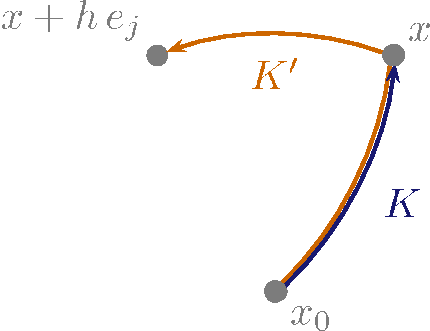
\includegraphics[scale=0.2]{images/ana3-tmp-49}
  \end{figure}
  %
  Falls $G = \mathbb{C} \setminus ]-\infty,0]$
  %
  \begin{align*}
    f(z) = |z|^{1/N} \mathrm{e}^{\mathrm{i}\frac{1}{N}\arg z}
  \end{align*}
  %
  falls $G = \mathbb{C} \setminus ]-\mathrm{i} \infty,\mathrm{i} 0]$
  %
  \begin{align*}
    f(z) = |z|^{1/N} \mathrm{e}^{\mathrm{i}\frac{1}{N}\arg_{\pi/2} z}
  \end{align*}
\end{example}

\begin{notice}[Ausblick]
  Erweiterung des Wegintegrals auf stetige Kurven. Ist $f$ analytische fortsetzbar längs $\gamma$ mit Unterteilung \[ t_0 = \tau_0 < \tau_1 < \ldots < \tau_n = t_1 , \] so definiere
  %
  \begin{align*}
    \int_\gamma f(z) \, \mathrm{d}z &\coloneq \sum\limits_{j=1}^{\infty} \int_{\gamma|_{[\tau_{j-1},\tau_j]}} f(z) \, \mathrm{d}z \\
    \int_{\gamma|_{[\tau_{j-1},\tau_j]}} f(z) \, \mathrm{d}z &\coloneq F_j(\gamma(\tau_j)) - F_j(\gamma(\tau_{j-1})).
  \end{align*}
  %
  $F$ ist die lokale Stammfunktion der Fortsetzung von $f$ in $K_j$.
\end{notice}

%
% vim: ts=2:sw=2:expandtab
% Henri Menke, 2012 Universität Stuttgart.
%
% Dieses Werk ist unter einer Creative Commons Lizenz vom Typ
% Namensnennung - Nicht-kommerziell - Weitergabe unter gleichen Bedingungen 3.0 Deutschland
% zugänglich. Um eine Kopie dieser Lizenz einzusehen, konsultieren Sie
% http://creativecommons.org/licenses/by-nc-sa/3.0/de/ oder wenden Sie sich
% brieflich an Creative Commons, 444 Castro Street, Suite 900, Mountain View,
% California, 94041, USA.

\setcounter{thmn}{0}
\chapter{Vektoranalysis}

%
% Henri Menke, 2012 Universität Stuttgart.
%
% Dieses Werk ist unter einer Creative Commons Lizenz vom Typ
% Namensnennung - Nicht-kommerziell - Weitergabe unter gleichen Bedingungen 3.0 Deutschland
% zugänglich. Um eine Kopie dieser Lizenz einzusehen, konsultieren Sie
% http://creativecommons.org/licenses/by-nc-sa/3.0/de/ oder wenden Sie sich
% brieflich an Creative Commons, 444 Castro Street, Suite 900, Mountain View,
% California, 94041, USA.

\section{Kurvenintegrale}
\addtocounter{thmn}{1}
\setcounter{theorem}{0}

% % % Vorlesung vom 06.12.2012

\begin{theorem}[Definition]
  Sei $f \in C([a,b] \to \mathbb{R}^n)$.
  %
  \begin{enum-arab}
    \item $K \coloneq \mathrm{Bild}(f)$ heißt \acct{Kurve} im $\mathbb{R}^n$, $(f,[a,b])$ heißt \acct{Parameterdarstellung} von $K$. Ist $f(a) = f(b)$, so heißt $K$ geschlossen.

    \item Ist $f\Big|_{[a,b[}$ injektiv, so heißt $K$ \acct{Jordan-Kurve}.
  \end{enum-arab}
  %
  \begin{figure}[H]
    \centering
%    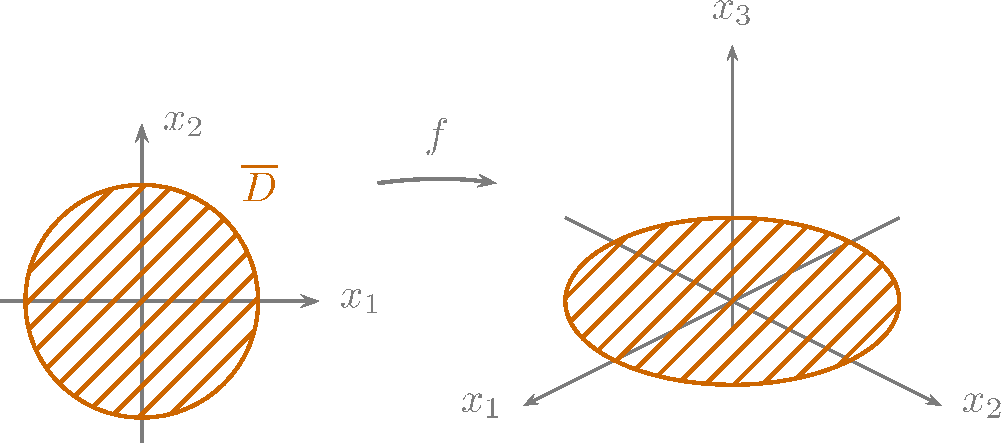
\includegraphics[scale=0.2]{images/ana3-tmp-50}
  \end{figure}
  %
  Diese Kurve ist geschlossen und nicht Jordan.
\end{theorem}

\begin{notice}
  Die Parameterdarastellung induziert den Durchlaufsinn.
\end{notice}

\begin{example} \label{thm:6.3}
  Für $r > 0$, $c > 0$ beschreibt
  %
  \begin{align*}
    f(t) = \begin{pmatrix} r \cos t \\ r \sin t \\ c t \end{pmatrix} \; , \quad 0 \leq t \leq 4 \pi
  \end{align*}
  %
  \begin{figure}[H]
    \centering
    %\psset{Alpha=0,Beta=0}
    \includegraphics[scale=0.2]{images/ana3-tmp-51}
  \end{figure}
  %
  eine Schraubenlinie mit Radius $r$ und Ganghöhe $\frac{c}{2 \pi}$.
\end{example}

\begin{theorem}[Definition]
  Seien $(f,[a,b])$ und $(g,[c,d])$ zwei Parameterdarstellungen von $K$. Existiert $\varphi \in C^1([a,b] \to \mathbb{R})$ mit
  %
  \begin{item-triangle}
    \item $\varphi'(t) > 0$ in $[a,b]$

    \item $\varphi(a) = c$, $\varphi(b) = d$

    \item $f(t) = (g \circ \varphi)(t)$, $t \in [a,b]$
  \end{item-triangle}
  %
  so heißen die Parameterdarstellungen \acct[0]{äquivalent}\index{Parameterdarstellung!äquivalent}.
\end{theorem}

\begin{example}
  \begin{enum-arab}
    \item Die Parameterdarstellung
    %
    \begin{align*}
      g(t) = \begin{pmatrix} r \cos \left( 8 \pi \frac{t}{1 + t} \right) \\ r \sin \left( 8 \pi \frac{t}{1 + t} \right) \\ c \left( 8 \pi \frac{t}{1 + t} \right) \end{pmatrix} \; , \quad 0 \leq t \leq 1
    \end{align*}
    %
    ist äquivalent zu $f$ aus \ref{thm:6.3} (mit $\varphi(t) = 8 \pi \frac{t}{1 + t}$).

    \item Die Parameterdarstellung
    %
    \begin{align*}
      h(t) = \begin{pmatrix} r \cos t^2 \\ r \sin t^2 \\ c t^2 \end{pmatrix} \; , \quad 0 \leq t \leq \sqrt{4 \pi}
    \end{align*}
    %
    ist nicht äquivalent zu $f$ aus \ref{thm:6.3} ($\varphi(t) = t^2$), weil $\varphi'(0) = 0$.
  \end{enum-arab}
\end{example}

\begin{theorem}[Definition]
  Sei $(f,[a,b])$ Parameterdarstellung von $K$. Existiert $f'(t_0)$ und ist $f'(t_0) \neq 0$, so heißt
  %
  \begin{align*}
    T_f(t_0) \coloneq \frac{1}{\|f'(t_0)\|} f'(t_0)
  \end{align*}
  %
  \acct{Tangenteneinheitsvektor} an $K$ im Punkt $f(t_0)$.
  %
  \begin{figure}[H]
    \centering
    \includegraphics[scale=0.2]{images/ana3-tmp-52}
  \end{figure}
\end{theorem}

\begin{theorem}[Satz]
  Sind $(f,[a,b])$ und $(g,[c,d])$ äquivalente Parameterdarstellungen von $K$, so gilt
  %
  \begin{align*}
    T_f(t) &= \frac{f'(t)}{\|f'(t)\|} = \frac{(g \circ \varphi)'(t)}{\|(g \circ \varphi)'(t)\|} \\
    &= \frac{g'(\varphi(t)) \varphi'(t)}{\|g'(\varphi(t)) \varphi'(t)\|} \overset{\varphi'(t) > 0}{=} \frac{g'(\varphi(t))}{\|g'(\varphi(t))\|} \\
    &= T_g(\varphi(t))
  \end{align*}
\end{theorem}

\begin{theorem}[Definition]
  Sei $K$ eine Kurve im $\mathbb{R}^n$.
  %
  \begin{enum-arab}
    \item Existiert eine Parameterdarstellung $(f,[a,b])$ mit $f \in C^1([a,b] \to \mathbb{R}^n)$ und $f'(t) \neq 0$ auf $[a,b]$, so heißt $K$ \acct[0]{glatt}\index{Kurve!glatt}. Insbesondere ist dann $T_f$ stetig.

    \item $K$ heißt \acct[0]{stückweise glatt}\index{Kurve!stückweise glatt}, falls es eine Parameterdarstellung $(f,[a,b])$ gibt und eine Unterteilung $a=t_0 < t_1 < \ldots < t_n=b$, sodass die Teilkurven von $K$ glatt sind:
    %
    \begin{align*}
      f\Big|_{[t_{j-1},t_j]} \in C^1([t_{j-1},t_j] \to \mathbb{R}^n)
    \end{align*}
    %
    und $f'(t) \neq 0$ für $t_{j-1} \leq t \leq t_j$.
  \end{enum-arab}
\end{theorem}

\begin{notice}
  Glatte Kurven haben keine Ecken, stückweise glatte Kurven können Ecken besitzen.
\end{notice}

\begin{theorem}[Definition]
  Sei $K$ eine Jordan-Kurve mit der Parameterdarstellung $(f,[a,b])$.
  %
  \begin{enum-arab}
    \item Falls
    %
    \begin{gather*}
      \exists \, M > 0 \, \forall \, m \in \mathbb{N} \, \forall \, a=t_0 < t_1 < \ldots < t_n=b : \\ \quad L_{\{t_0,\ldots,t_n\}}(K) \coloneq \sum\limits_{j=1}^{n} \left\| f(t_j) - f(t_{j-1}) \right\| \leq M
    \end{gather*}
    %
    so heißt $K$ \acct[0]{rektifizierbar}. \index{Kurve!rektifizierbar}

    \begin{figure}[H]
      \centering
%      \includegraphics[scale=0.2]{images/ana3-tmp-53}
    \end{figure}

    \item Ist $K$ rektifizierbar, so heißt
    %
    \begin{align*}
      L(K) \coloneq \sup\limits_{n \in \mathbb{N}} L_{\{t_0,\ldots,t_n\}}(K)
    \end{align*}
    %
    die \acct[0]{Bogenlänge}\index{Kurve!Bogenlänge} von $K$.
  \end{enum-arab}
\end{theorem}

\begin{theorem}[Satz] \label{thm:6.11}
  Sei $K$ glatte Jordan-Kurve mit Parameterdarstellung $(f,[a,b])$, $f \in C^1([a,b] \to \mathbb{R}^n)$. Dann ist $K$ rektifizierbar und es gilt
  %
  \begin{align*}
    L(K) = \int\limits_{a}^{b} \|f'(t)\| \, \mathrm{d}t
  \end{align*}

  \begin{proof}
    \begin{enum-arab}
      \item Für $a=t_0 < t_1 < \ldots < t_n=b$ gilt
      %
      \begin{align*}
        \|f(t_j) - f(t_{j-1})\|
        &= \left\| \int\limits_{t_{j-1}}^{t_j} f'(t) \, \mathrm{d}t \right\|
        \leq \int\limits_{t_{j-1}}^{t_j} \|f'(t)\| \, \mathrm{d}t \\
        \implies L_{\{t_0,\ldots,t_n\}}(K)
        &\leq \int\limits_{a}^{b} \|f'(t)\| \, \mathrm{d}t \eqcolon M \\
        L(K) &\leq M
      \end{align*}
      %
      $\implies$ $K$ ist rektifizierbar.

      \item Sei $\varepsilon > 0$ fest. $f'$ gleichmäßig stetig
      %
      \begin{align*}
        \implies \quad \exists \, \delta > 0 \, \forall \, |s-t| < \delta : \|f'(s) - f'(t)\| < \varepsilon
      \end{align*}
      %
      Sei $a=t_0 < t_1 < \ldots < t_n=b$ mit $\max|t_j - t_{j-1}| < \delta$
      %
      \begin{align*}
        \implies \quad \|f'(t)\|
        &= \|f'(t) - f'(t_j) + f'(t_j)\| \\
        &\leq \varepsilon + \|f'(t_j)\| \quad \text{für } t_{j-1} \leq t \leq t_j \\
        \implies \quad \int\limits_{t_{j-1}}^{t_j} \|f'(t)\| \, \mathrm{d}t
        &\leq \varepsilon (t_j - t_{j-1}) + \|f'(t_j)\| (t_j - t_{j-1}) \\
        &= \varepsilon (t_j - t_{j-1}) + \left\| \int\limits_{t_{j-1}}^{t_j} \left( f'(t_j) - f'(t) + f'(t) \right) \, \mathrm{d}t \right\| \\
        &\leq 2 \varepsilon (t_j - t_{j-1}) + \|f'(t_j) - f'(t_{j-1})\| \\
        \overset{\sum_j}{\implies} \int\limits_{a}^{b} \|f'(t)\| \, \mathrm{d}t
        &\leq 2 \varepsilon (b-a) + L_{\{t_0,\ldots,t_n\}} (K) \\
        &\leq 2 \varepsilon (b-a) + L (K) \\
        \overset{\varepsilon \downarrow 0}{\implies} \int\limits_{a}^{b} \|f'(t)\| \, \mathrm{d}t &\leq L(K)
      \end{align*}
    \end{enum-arab}
  \end{proof}
\end{theorem}

% % % Vorlesung vom 10.12.2012

\begin{theorem}[Hilfssatz] \label{thm:6.12}
  Sei $K$ eine rektifizierbare Jordan-Kurve mit Parameterdarstellung $(\gamma,[a,b])$. Ist $a < c < b$, $K' = \gamma([a,c])$, $K'' = \gamma([c,b])$, dann sind $K'$, $K''$ rektifizierbare Jordan-Kurven und es gilt $L(K') + L(K'') = L(K)$.

  \begin{proof}
    \begin{enum-arab}
      \item Seien $a = t_0 < t_1 < \ldots < t_n = c$ und $c = s_0 < s_1 < \ldots < s_n = b$.
      %
      \begin{align*}
        \implies
        \underbrace{L_{\{t_0,\ldots,t_n\}}(K')}_{\geq 0}
        + \underbrace{L_{\{s_0,\ldots,s_n\}}(K'')}_{\geq 0}
        &= L_{\{t_0,\ldots,t_n=s_0,\ldots,s_n\}}(K) \\
        &\geq L(K)
      \end{align*}
      %
      $\implies$ $K'$,$K''$ sind rektifizierbar, $L(K') + L(K'') \leq L(K)$.

      \item Sei $\varepsilon > 0$ gegeben, $\{t_0,\ldots,t_n\}$ mit
      %
      \begin{align*}
        L_{\{t_0,\ldots,t_n\}}(K) \geq L(K) - \varepsilon
      \end{align*}
      %
      Füge eventuell $c$ als Unterteilungspunkt dazu. \[\{t_0' = a < t_1' < \ldots < t_k' = c < t_{k+1}' < \ldots < t_m' = b\}\] Wegen der Dreiecksungleichung
      %
      \begin{align*}
        L_{\{t_0',\ldots,t_m'\}}(K) \geq L_{\{t_0,\ldots,t_n\}}(K) \geq L(K) - \varepsilon
      \end{align*}
      %
      wegen
      %
      \begin{align*}
        \|\gamma(t_{k+1}')-\gamma(t_{k-1}')\| &= \|\gamma(t_{k+1}')-\gamma(t_{k}')\| + \|\gamma(t_{k}')-\gamma(t_{k-1}')\|.
      \end{align*}
      %
      Außerdem
      %
      \begin{align*}
        L_{\{t_0',\ldots,t_m'\}}(K) = L_{\{t_0',\ldots,t_k'\}}(K') + L_{\{t_k',\ldots,t_m'\}}(K'')
      \end{align*}
      %
      damit folgt
      %
      \begin{align*}
        L(K') + L(K'') \geq L(K) - \varepsilon
      \end{align*}
      %
      da $\varepsilon > 0$ beliebig $L(K') + L(K'') \geq L(K)$.

      \begin{figure}[H]
        \centering
        \includegraphics[scale=0.2]{images/ana3-tmp-54}
      \end{figure}
    \end{enum-arab}
  \end{proof}
\end{theorem}

\begin{notice}
  Ist $K$ eine rektifizierbare Jordan-Kurve mit äquivalenten Parameterdarstellungen $f$ und $g$, so gilt
  %
  \begin{align*}
    L^{(f)}(K)
    &= \sup\limits_{\{\ldots\}} \sum\limits_{j=1}^{n} \|f(t_j) - f(t_{j-1})\| \\
    &= \sup\limits_{\{\ldots\}} \sum\limits_{j=1}^{n} \|g(s_j) - g(s_{j-1})\| \\
    &= L^{(g)}(K)
  \end{align*}
  %
  denn zu $\{t_0,\ldots,t_n\}$ >>passt<< genau die Unterteilung $\{\varphi^{-1}(t_0),\ldots,\varphi^{-1}(t_n)\}$ und umgekehrt.
\end{notice}

\begin{theorem}[Hilfssatz] \label{thm:6.14}
  Sei $K$ eine rektifizierbare Jordan-Kurve mit der Parameterdarstellung $(\gamma,[a,b])$. Definiere $L : [a,b] \to \mathbb{R}$ durch
  %
  \begin{align*}
    L(t) \coloneq L(K_t) \; , \quad K_t \coloneq \gamma([a,t]) , \; a \leq t \leq b
  \end{align*}
  %
  \begin{figure}[H]
    \centering
    \includegraphics[scale=0.2]{images/ana3-tmp-55}
  \end{figure}
  %
  Dann gelten:
  %
  \begin{enum-arab}
    \item $L$ ist streng monoton wachsend

    \item $L$ ist stetig

    \item $\mathrm{Bild}(L) = [0,L(K)]$

    \item Falls $K$ glatt ist und $\gamma \in C^1$, dann ist $L$ differenzierbar und \[L'(t) = \|\gamma'(t)\|\]
  \end{enum-arab}

  \begin{proof}
    \begin{enum-arab}
      \item \label{itm:6.14 1)} Sei $a \leq t < s \leq b$.
      %
      \begin{align*}
        L(s) &\overset{\text{\ref{thm:6.12}}}{=} L(t) + L(K') \; , \quad K' = \gamma([t,s]) \\
        L(K') &\geq \|\gamma(s) - \gamma(t)\| > 0
      \end{align*}
      %
      da $K$ Jordan-Kurve und $s,t$ nicht zugleich Anfangs- und Endpunkt.

      \item \label{itm:6.14 2)}
      \begin{enumerate}
        \item \label{itm:6.14 2)a}Zeige: $L$ ist stetig in $t=b$. Sei $\varepsilon > 0$. Wähle $a = t_0 < \ldots < t_n = b$ mit $L_{\{t_0,\ldots,t_n\}}(K) > L(K) - \varepsilon$ {\color{DarkRed} $(*)$}. $\gamma$ ist gleichmäßig stetig, wenn gilt
        %
        \begin{align*}
          \exists \, \delta > 0 : |s-t| < \delta \implies |\gamma(s) - \gamma(t)| < \frac{\varepsilon}{2} \tag*{\color{DarkGreen} $(**)$}
        \end{align*}
        %
        Setze $K_j \coloneq \gamma([t_j,t_{j-1}])$
        %
        \begin{gather*}
          \overset{\text{\ref{thm:6.12}}}{\implies} \sum\limits_{j=1}^{n} L(K_j) = L(K) \\
          \begin{aligned}
            \implies 0 &\leq L(K_n) - \|\gamma(t_n)-\gamma(t_{n-1})\|
            \leq \sum\limits_{j=1}^{n} \Big( \underbrace{L(K_j) - \|\gamma(t_j)-\gamma(t_{j-1})\|}_{\geq 0} \Big) \\
            &= L(K) - L_{\{t_0,\ldots,t_n\}}(K) < \frac{\varepsilon}{2}
          \end{aligned}
        \end{gather*}
        %
        O.B.d.A. kann angenommen werden:
        %
        \begin{align*}
          |t_j - t_{j-1}| < \delta
        \end{align*}
        %
        Andernfalls füge geeignet weitere Unterteilungspunkt hinzu. Da dabei $L_{\{\ldots\}}(K)$ höchstens größer wird bleibt {\color{DarkRed} $(*)$} erhalten.
        %
        \begin{align*}
          \implies L(K_n) &\leq \frac{\varepsilon}{2} + \|\gamma(t_n) - \gamma(t_{n-1})\| \overset{\color{DarkGreen} (**)}{<} \varepsilon \\
          \implies 0 &\overset{\text{\ref{itm:6.14 1)}}}{\leq} L(\ell = t_n) - L(t) \; , \quad \text{für } t_{n-1} \leq t \leq t_n = \ell \\
          &\overset{\text{\ref{itm:6.14 1)}}}{\leq} L(\ell) - L(t_{n-1}) \\
          &= L(K_n) \\
          &< \varepsilon
        \end{align*}
        %
        $\implies$ $L$ ist (linksseitig) stetig bei $t=b$.

        \item \label{itm:6.14 2)b} Für $t \in ]a,b]$ betrachte $\gamma([a,t])$. Wende a) an, dann folgt, dass $L$ linksseitig stetig bei $t$ ist.

        \item \label{itm:6.14 2)c} Rechtsseitige Stetigkeit bei $t = a$: Wie \ref{itm:6.14 2)a}, aber $K_1$ anstelle von $K_n$:
        %
        \begin{align*}
          0 &\leq L(K_1) - \|\gamma(t_1) - \gamma(t_0 = a)\| \leq \ldots \leq \frac{\varepsilon}{2} \\
          \implies L(K_1) &< \varepsilon
        \end{align*}

        \item Für $t \in [a,b[$ betrachte $\gamma([t,b])$, wende \ref{itm:6.14 2)c} an $\implies$ $L$ rechtsseitig stetig in $t$.
      \end{enumerate}

      \item Klar.

      \item $\displaystyle L(t) \overset{\text{\ref{thm:6.11}}}{=} \int\limits_{a}^{t} \|\underbrace{\gamma'(\tau)}_{\text{stetig}}\| \, \mathrm{d}\tau \implies L'(t) = \|\gamma'(t)\|$
    \end{enum-arab}
  \end{proof}
\end{theorem}

\begin{theorem}[Definition]
  Sei $K$ eine rektifizierbare Jordan-Kurve mit der Parameterdarstellung $(\gamma,[a,b])$. Dann heißt
  %
  \begin{align*}
    (g,[0,L(K)]) \; , \quad \text{mit } g(s) \coloneq \gamma(L^{-1}(s))
  \end{align*}
  %
  \acct{Bogenlängendarstellung} von $K$ (äquivalente Parameterdarstellungen führen auf dieselbe Bogenlängedarstellung).

  \begin{figure}[H]
    \centering
    \includegraphics[scale=0.2]{images/ana3-tmp-56}
  \end{figure}
  %
  Beide {\color{DarkOrange3} orangenen} Linien sind gleich lang.
\end{theorem}

\begin{notice}[Folgerung:]
  Falls $K$ glatt und $\gamma$ differenzierbar folgt aus \ref{thm:1.14} 4.), dass $L$ differenzierbar ist. Wegen
  %
  \begin{align*}
    (L^{-1})'(s) = \frac{1}{L'(L^{-1}(s))} = \frac{1}{\|\gamma'(L^{-1}(s))\|} \neq 0 \text{, da $K$ glatt ist}
  \end{align*}
  %
  ergibt sich für die Bogenlängendarstellung von $K$
  %
  \begin{align*}
    \|g'(s)\| = \|\gamma'(L^{-1}(s)) \, {L^{-1}}'(s)\| = 1
  \end{align*}
\end{notice}

\begin{example}
  Sei eine Kurve durch die Parametrisierung $\gamma$ gegeben:
  \begin{align*}
    \gamma(t) &= r \begin{pmatrix} \cos(2 \pi t) \\ \sin(2 \pi t) \end{pmatrix} \; , \quad 0 \leq t \leq 1 \\
    \|\gamma'(t)\| &= \left\| r \begin{pmatrix} -2 \pi \sin(2 \pi t) \\ 2 \pi \cos(2 \pi t) \end{pmatrix} \right\| = 2 \pi r \\
    \implies L(t) &= \int\limits_{0}^{t} \|\gamma'(\tau)\| \, \mathrm{d}\tau = 2 \pi r t = s \\
    \implies L^{-1}(s) &= t = \frac{s}{2 \pi r}
  \end{align*}
  %
  Damit ergibt sich die Bogenlängendarstellung:
  %
  \begin{align*}
    g(s) = \gamma(L^{-1}(s)) = r \begin{pmatrix} \cos\frac{s}{r} \\ \sin\frac{s}{r} \end{pmatrix} \; , \quad 0 \leq s \leq 2 \pi r
  \end{align*}
\end{example}

\begin{theorem}[Definition]
  Sei $K$ eine rektifizierbare Jordan-Kurve mit Bogenlängendarstellung $(g, [0,L(K)])$, $f : D \subseteq \mathbb{R}^n \to \mathbb{R}$ stetig, $K \subseteq D$. Dann heißt
  %
  \begin{align*}
    \int_K f \, \mathrm{d}s \coloneq \int\limits_{0}^{L(K)} f(g(s)) \, \mathrm{d}s
  \end{align*}
  %
  \acct{Kurvenintegral von $f$ über $K$}.
\end{theorem}

\begin{theorem}[Satz]
  Sei $K$ eine glatte, rektifizierbare Jordan-Kurve, $f : D \subseteq \mathbb{R}^n \to \mathbb{R}$ stetig, $K \subseteq D$ und $(\gamma,[a,b])$ die Parameterdarstellung von $K$. Dann
  %
  \begin{align*}
    \int_K f \, \mathrm{d}s = \int\limits_{a}^{b} f(\gamma(t)) \, \|\gamma'(t)\| \, \mathrm{d}t
  \end{align*}

  \begin{proof}
    \begin{align*}
      \int_K f \, \mathrm{d}s &= \int\limits_{0}^{L(K)} f(g(s)) \, \mathrm{d}s
    \intertext{Nebenrechnung}
      g &= \gamma \circ L^{-1}
    \intertext{Substitution: $s = L(t)$}
      \frac{\mathrm{d}s}{\mathrm{d}t} &= L'(t) = \|\gamma'(t)\|
    \intertext{Einsetzen}
      &\overset{s=L(t)}{=} \int\limits_{0=L(a)}^{L(K)=L(b)} f(g(L(t))) \, \|\gamma'(t)\| \, \mathrm{d}t \\
      &= \int\limits_{a}^{b} f(\gamma(t)) \, \|\gamma'(t)\| \, \mathrm{d}t
    \end{align*}
  \end{proof}
\end{theorem}

\begin{example}
  \begin{enum-arab}
    \item $\gamma : [a,b] \to \mathbb{R}^1 : t \mapsto t$
    %
    \begin{align*}
      \implies& K = [a,b] \\
      \implies& \int_K f \, \mathrm{d}s = \int\limits_{a}^{b} f(\gamma(t)) \, 1 \, \mathrm{d}t
    \end{align*}
    %
    Also: Kurvenintegral beinhaltet >>altes<< Integral über Intervalle.

    \item $\gamma(t) = \begin{pmatrix} t \\ a t \end{pmatrix}, \; 0 \leq t \leq 1$, $f(x,y) = x^2 + y^2$
    %
    \begin{align*}
      \int_K f \, \mathrm{d}s = \int\limits_{0}^{1} (t^2 + a^2 t^2) \, \sqrt{1 + a^2} \, \mathrm{d}t = \frac{1}{3} (1+a^2)^{3/2}
    \end{align*}
  \end{enum-arab}
\end{example}

% % % Vorlesung vom 13.12.2012

\begin{notice}[Eigenschaften von Kurvenintegralen:]
  \begin{enum-arab}
    \item Linearität:
    %
    \begin{align*}
      \int_K (\lambda \, f + \mu \, g) \, \mathrm{d}s = \lambda \int_K f \, \mathrm{d}s + \mu \int_K g \, \mathrm{d}s
    \end{align*}

    \item \acct{Standardabschätzung}:
    \begin{align*}
      \left| \int_K f \, \mathrm{d}s \right| \leq \max\limits_{x \in K} |f(x)| \, L(K)
    \end{align*}

    \item Sei $K = K_1 \cup K_2$, dann
    \begin{align*}
      \int_K f \, \mathrm{d}s = \int_{K_1} f \, \mathrm{d}s + \int_{K_2} f \, \mathrm{d}s
    \end{align*}
  \end{enum-arab}
\end{notice}

\begin{theorem}[Definition]
  \begin{enum-arab}
    \item Seien $f : D \subseteq \mathbb{R}^n \to \mathbb{R}^n$, $D$ offen, $f$ differenzierbar. Dann heißt
    %
    \begin{align*}
      \mathrm{div}\, f = \nabla \cdot f =
      \begin{pmatrix} \partial_{x_1} \\ \vdots \\ \partial_{x_n} \end{pmatrix}
      \cdot
      \begin{pmatrix} f_1 \\ \vdots \\ f_n \end{pmatrix}
      =
      \sum\limits_{j=1}^{n} \partial_{x_j} f_j
    \end{align*}
    %
    \acct{Divergenz}\index{Vektorfeld!Divergenz} von $f$ (Quellenstärke). In diesem Zusammenhang heißt $f$ auch \acct{Vektorfeld}.

    \item Seien $f : D \subseteq \mathbb{R}^n \to \mathbb{R}$, $D$ offen, $f$ differenzierbar. Dann heißt
    %
    \begin{align*}
      \mathrm{grad}\, f = \nabla f = \begin{pmatrix} \partial_{x_1} \\ \vdots \\ \partial_{x_n} \end{pmatrix} f = \begin{pmatrix} \partial_{x_1} f \\ \vdots \\ \partial_{x_n} f \end{pmatrix}
    \end{align*}
    %
    \acct{Gradient}\index{Vektorfeld!Gradient} von $f$. Man nennt $f$ auch \acct{Skalarfeld}\index{Vektorfeld!Skalarfeld}.

    \item Seien $f : D \subseteq \mathbb{R}^n \to \mathbb{R}^n$ ein Vektorfeld und $D$ offen. Gibt es eine Funktion $F : D \to \mathbb{R}$, sodass \[ \nabla F = f \text{ in } D \] so heißt $f$ \acct{Gradientenfeld}\index{Vektorfeld!Gradientenfeld}, $F$ heißt \acct{Potential}\index{Vektorfeld!Potential} von $f$.

    \item Seien $f : D \subseteq \mathbb{R}^3 \to \mathbb{R}^3$, $f$ differenzierbar. Dann heißt
    %
    \begin{align*}
      \mathrm{rot}\, f = \nabla \times f =
      \begin{pmatrix} \partial_{x_1} \\ \partial_{x_2} \\ \partial_{x_3} \end{pmatrix}
      \times
      \begin{pmatrix} f_1 \\ f_2 \\ f_3 \end{pmatrix}
      =
      \begin{pmatrix} \partial_{x_2} f_3 - \partial_{x_3} f_2 \\ \partial_{x_3} f_1 - \partial_{x_1} f_3 \\ \partial_{x_1} f_2 - \partial_{x_2} f_1 \end{pmatrix}
    \end{align*}
    %
    \acct{Rotation}\index{Vektorfeld!Rotation} von $f$ (Wirbelstärke).
  \end{enum-arab}
\end{theorem}

\begin{notice}[Rechenregeln:]
  Seien im Folgenden $f,g : \mathbb{R}^n \to \mathbb{R}^n$, $f_3,g_3 : \mathbb{R}^3 \to \mathbb{R}^3$ Vektorfelder, $a,b : \mathbb{R}^n \to \mathbb{R}$ Skalarfelder und $\lambda, \mu \in \mathbb{R}$ Skalare.
  \begin{enum-arab}
    \item Linearität:
    \begin{align*}
      \nabla \cdot (\lambda \, f + \mu \, g) &= \lambda \, \nabla \cdot f + \mu \, \nabla \cdot g \\
      \nabla \, (\lambda \, f + \mu \, g) &= \lambda \, \nabla \, f + \mu \, \nabla \, g \\
      \nabla \times (\lambda \, f_3 + \mu \, g_3) &= \lambda \, \nabla \times f_3 + \mu \, \nabla \times g_3
    \end{align*}

    \item Produktregeln:
    \begin{align*}
      \nabla \cdot (a \, f) &= (\nabla \, a) \cdot f + a \, \nabla \cdot f \\
      \nabla (a \, b) &= a \, \nabla \, b + b \, \nabla \, a \\
      \nabla \times (a \, f) &= a \, (\nabla \times f) + (\nabla \, a) \times f
    \end{align*}

    \item
    \begin{align*}
      \nabla \times (\nabla \, f_3) &= 0 \\
      \nabla \cdot (\nabla \times f_3) &= 0
    \end{align*}
  \end{enum-arab}
\end{notice}

\begin{theorem}[Definition]
  Sei $K$ eine glatte Jordan-Kurve mit der Parameterdarstellung $(\gamma,[a,b])$, $f : D \subseteq \mathbb{R}^n \to \mathbb{R}^n$ stetig, $K \subseteq D$. Dann heißt
  %
  \begin{align*}
    \int_K f \cdot T \, \mathrm{d}s \coloneq \int\limits_{a}^{b} f(\gamma(t)) \cdot \gamma'(t) \, \mathrm{d}t
  \end{align*}
  %
  das \acct{Wegintegral} von $f$ über $K$.
\end{theorem}

\begin{notice}
  \begin{enum-arab}
    \item Die Definition ergibt durchaus ihren Sinn, denn aus der Definition des bekannten Kurvenintegrals erhält man:
    %
    \begin{align*}
      \int_K f \cdot T \, \mathrm{d}s = \int\limits_{a}^{b} \left( f(\gamma(t)) \cdot \frac{\gamma'(t)}{\|\gamma'(t)\|} \right) \|\gamma'(t)\| \, \mathrm{d}t = \int\limits_{a}^{b} f(\gamma(t)) \cdot \gamma'(t) \, \mathrm{d}t
    \end{align*}

    \item Das Wegintegral wird in der Physik auch als Arbeitsintegral bezeichnet.
    %
    \begin{align*}
      W = \int \bm{F}(\bm{r}) \, \frac{\partial \bm{r}(t)}{\partial t} \, \mathrm{d}t
    \end{align*}

    \item Andere Schreibweise
    %
    \begin{align*}
      \int_K f \cdot T \, \mathrm{d}s &= \sum\limits_{j=1}^{n} \int_K f_j \, \mathrm{d}x_j \\
      \int_K f_j \, \mathrm{d}x_j &= \int\limits_{a}^{b} f_j(\gamma(t)) \cdot \gamma_j'(t) \, \mathrm{d}t
    \end{align*}
  \end{enum-arab}
\end{notice}

\begin{theorem}[Satz] \label{thm:6.26}
  Ist $f : D \to \mathbb{R}^n$ ein Gradientenfeld mit Potential $F : D \to \mathbb{R}$, so gilt für jede Kurve $K \subseteq D$
  %
  \begin{align*}
    \int_K f \cdot T \, \mathrm{d}s = F(\text{Endpunkt}) - F(\text{Anfangspunkt})
  \end{align*}
  %
  Insbesondere: Wegintegral ist wegunabhängig.

  \begin{proof} Betrachte
    \begin{align*}
      \int_K f \cdot T \, \mathrm{d}s &= \int_K f(\gamma(t)) \cdot \gamma'(t) \, \mathrm{d}t
    \intertext{wobei $f(\gamma(t)) = \nabla F(\gamma(t))$}
      &= \int\limits_{a}^{b} \frac{\mathrm{d}}{\mathrm{d}t} (F \circ \gamma)(t) \, \mathrm{d}t
   \intertext{mit der Kettenregel}
     \frac{\mathrm{d}}{\mathrm{d}t} (F \circ \gamma)(t) &= \sum\limits_{j=1}^{n} \partial_{x_j} F(\gamma(t)) \cdot \gamma_j'(t)
   \intertext{mit dem Hauptsatz der Differential und Integralrechnung}
     \int_K f \cdot T \, \mathrm{d}s &= (F \circ \gamma)(b) - (F \circ \gamma)(a) \\
     &= F(\gamma(b)) - F(\gamma(a))
    \end{align*}
  \end{proof}
\end{theorem}

\begin{theorem}[Satz]
  Sei $D \subseteq \mathbb{R}^n$ ein Gebiet, $f \in C(D \to \mathbb{R}^n)$. Ist das Wegintegral über stückweise glatte Kurven in $D$ wegunabhängig, so besitzt $f$ ein Potential in $D$.

  \begin{proof}
    Sei $x_0 \in D$ fest. Zu $x \in D$ wähle eine Kurve $K$ von $x_0$ nach $x$, setze
    %
    \begin{align*}
      F(x) \coloneq \int_K f \cdot T \, \mathrm{d}s
    \end{align*}
    %
    Da das Integral wegunabhängig ist, ist $F$ sinnvoll definiert. Sei $j = \{1,\ldots,n\}$, $x \in D$.

    \begin{figure}[H]
      Vorüberlegung

      \centering
      \includegraphics[scale=0.2]{images/ana3-tmp-57}
    \end{figure}

    \begin{align*}
      F(x + h \, e_j) - F(x)
      &= \int\limits_{x}^{x + h \, e_j} f \cdot T \, \mathrm{d}s \\
      &= \int\limits_{0}^{h} f(x + t \, e_j) \cdot e_j \, \mathrm{d}t \\
      &= \int\limits_{0}^{h} f_j(x + t \, e_j) \, \mathrm{d}t
    \end{align*}

    \begin{align*}
      \left| \frac{1}{h} ( F(x + h \, e_j) ) - F(x) - f_j \right|
      &= \bigg| \frac{1}{h} \int\limits_{0}^{h} \underbrace{\left( f_j(x + t \, e_j) - f_j(x) \right)}_{|\cdot| < \varepsilon \text{ für } |h| < \delta} \, \mathrm{d}t \bigg| \\
      &< \frac{1}{h} \, \varepsilon \, h = \varepsilon \text{ für } |h| < \delta
    \end{align*}
  \end{proof}
\end{theorem}

%
% Henri Menke, 2012 Universität Stuttgart.
%
% Dieses Werk ist unter einer Creative Commons Lizenz vom Typ
% Namensnennung - Nicht-kommerziell - Weitergabe unter gleichen Bedingungen 3.0 Deutschland
% zugänglich. Um eine Kopie dieser Lizenz einzusehen, konsultieren Sie
% http://creativecommons.org/licenses/by-nc-sa/3.0/de/ oder wenden Sie sich
% brieflich an Creative Commons, 444 Castro Street, Suite 900, Mountain View,
% California, 94041, USA.

\section{Flächenintegrale im \texorpdfstring{$\mathbb{R}^3$}{R\textsuperscript{3}}}
\addtocounter{thmn}{1}
\setcounter{theorem}{0}

% % % Vorlesung vom 13.12.2012

\begin{theorem}[Definition]
  Sei $D \subseteq \mathbb{R}^2$ ein Gebiet, $f \in C^1(\overline{D} \to \mathbb{R}^3)$, $f|_D$ injektiv und
  %
  \begin{align*}
    \mathrm{Rang}\begin{pmatrix} \partial_{x_1} f(x) & \partial_{x_2} f(x) \end{pmatrix}
    = \mathrm{Rang}
    \begin{pmatrix}
      \partial_{x_1} f_1 & \partial_{x_2} f_1 \\
      \partial_{x_1} f_2& \partial_{x_2} f_2 \\
      \partial_{x_1} f_3 & \partial_{x_2} f_3 \\
    \end{pmatrix}
    = 2
  \end{align*}
  %
  für $x \in \overline{D}$. Dann heißt
  %
  \begin{align*}
    F \coloneq \mathrm{Bild}(f)
  \end{align*}
  %
  \acct{Fläche im $\mathbb{R}^3$}, $(f,\overline{D})$ heißt Parameterdarstellung von $f$.
\end{theorem}

\begin{theorem}[Satz]
  Ist $(\gamma,[a,b])$ Parameterdarstellung einer glatten Kurve in $\overline{D} \subset \mathbb{R}^2$, so ist $(f \circ \gamma,[a,b])$ eine glatte Kurve im $\mathbb{R}^3$.

  \begin{proof}
    \begin{enum-arab}
      \item $\gamma \in C^1$, $f \in C^1 \implies f \circ \gamma \in C^1$.

      \item
      \begin{align*}
        (f \circ \gamma)'(t) &=
        \begin{pmatrix}
          (f_1 \circ \gamma)'(t) \\
          (f_2 \circ \gamma)'(t) \\
          (f_3 \circ \gamma)'(t) \\
        \end{pmatrix} \\
        &=
        \begin{pmatrix}
          (\partial_{x_1} f_1) \gamma_1' + (\partial_{x_2} f_1) \gamma_2' \\
          (\partial_{x_1} f_2) \gamma_1' + (\partial_{x_2} f_2) \gamma_2' \\
          (\partial_{x_1} f_3) \gamma_1' + (\partial_{x_2} f_3) \gamma_2' \\
        \end{pmatrix} \\
        &= \gamma_1'(t) \partial_{x_1} f(\gamma(t)) + \gamma_2'(t) \partial_{x_2} f(\gamma(t)) \\
        &\neq 0
      \end{align*}
      %
      da $\{ \partial_{x_1} f, \partial_{x_2} f \}$ linear unabhängig und $\left(\begin{smallmatrix} \gamma_1' \\ \gamma_2' \end{smallmatrix}\right) \neq 0$.
    \end{enum-arab}
  \end{proof}
\end{theorem}

\begin{notice}[Folgerung:]
  Der Tangenteneinheitsvektor von $f \circ \gamma$ an der Stelle $t_0 \in [a,b]$:
  %
  \begin{align*}
    T_{f \circ \gamma}(t_0) = \frac{(f \circ \gamma)'(t_0)}{\| (f \circ \gamma)'(t_0) \|} = c_1 \partial_{x_1} f(\gamma(t_0)) + c_2 \partial_{x_2} f(\gamma(t_0))
  \end{align*}
  %
  liegt immer in der von $\{ \partial_{x_1} f, \partial_{x_2} f \}$ aufgespannten Ebene durch $f(\gamma(t_0))$.
\end{notice}

\begin{theorem}[Definition]
  Sei $(f,\overline{D})$ Parameterdarstellung einer Fläche $F$.
  %
  \begin{enum-arab}
    \item Für $x \in D$ heißt die Ebene \[ \{ f(x) + t \partial_{x_1} f(x) + s \partial_{x_2} f(x) : s,t \in \mathbb{R} \} \] die \acct{Tangentialebene} an $F$ im Punkt $f(x)$.

    \item Der \acct{Normaleneinheitsvektor} im Punkt $f(x)$ an die Fläche $F$ ist gegeben durch
    %
    \begin{align*}
      n(x) \coloneq \frac{\partial_{x_1} f(x) \times \partial_{x_2} f(x)}{\| \partial_{x_1} f(x) \times \partial_{x_2} f(x) \|}
    \end{align*}
  \end{enum-arab}
\end{theorem}

\begin{notice}
  $\| \partial_{x_1} f(x) \times \partial_{x_2} f(x) \|$ ist der Flächeninhalt des Parallelogramms, das von den beiden Vektoren $\partial_{x_1} f(x)$ und $\partial_{x_2} f(x)$ aufgespannt wird.
\end{notice}

\begin{theorem}[Definition]
  Sei $(f,\overline{D})$ Parameterdarstellung einer Fläche $F$ und $g \in C(\overline{D} \to \mathbb{R})$.
  %
  \begin{enum-arab}
    \item
    %
    \begin{align*}
      |F| \coloneq \int_{\overline{D}} \| \partial_{x_1} f(x) \times \partial_{x_2} f(x) \| \, \mathrm{d}x
    \end{align*}
    %
    heißt \acct{Flächeninhalt der Fläche $F$}.

    \item
    %
    \begin{align*}
      \int_{\overline{D}} g(f(x)) \cdot \| \partial_{x_1} f(x) \times \partial_{x_2} f(x) \| \, \mathrm{d}x \eqcolon \int_F g \, \mathrm{d}\sigma
    \end{align*}
    %
    heißt \acct{Integral} von $g$ über $F$. Offensichtlich
    %
    \begin{align*}
      \int_F 1 \, \mathrm{d}\sigma = |F|
    \end{align*}
  \end{enum-arab}
\end{theorem}

% % % Vorlesung vom 17.12.2012

\begin{example}
  \begin{align*}
    D &= \{ x \in \mathbb{R}^2 : |x| < \sqrt{2} \} \\
    f(x_1,x_2) &= \begin{pmatrix} x_1 \\ x_2 \\ 2 - x_1^2 - x_2^2 \end{pmatrix}
  \end{align*}

  \begin{figure}[H]
    \centering
    %\psset{Alpha=0,Beta=0}
    \includegraphics[scale=0.2]{images/ana3-tmp-58}
  \end{figure}

  \begin{align*}
    \partial_{x_1} f &= \begin{pmatrix} 1 \\ 0 \\ - 2 x_1 \end{pmatrix} \\
    \partial_{x_2} f &= \begin{pmatrix} 0 \\ 1 \\ - 2 x_2 \end{pmatrix} \\
    \| \partial_{x_1} f \times \partial_{x_1} f \| &= \left\| \begin{pmatrix} 1 \\ 0 \\ - 2 x_1 \end{pmatrix} \times \begin{pmatrix} 0 \\ 1 \\ - 2 x_2 \end{pmatrix} \right\| = \left\| \begin{pmatrix} 2 x_1 \\ 2 x_2 \\ 1 \end{pmatrix} \right\| \neq 0 \\
    |F| &= \int_{|x| < \sqrt{2}} \sqrt{1 + 4 |x|^2} \, \mathrm{d}x
  \intertext{Transformation auf Polarkoordinaten: $x = r \cos\varphi$, $y = r \sin\varphi$, $\mathrm{d}x = r \, \mathrm{d}r \, \mathrm{d}\varphi$}
    &= \int\limits_{\varphi = 0}^{2\pi} \int\limits_{r = 0}^{\sqrt{2}} \sqrt{1 + 4 r^2} \, r \, \mathrm{d}r \, \mathrm{d}\varphi \\
    &= \int\limits_{\varphi = 0}^{2\pi} \frac{1}{12} (1 + 4 r^2)^{3/2} \bigg|_{r=0}^{\sqrt{2}} \, \mathrm{d}\varphi \\
    &= \int\limits_{\varphi = 0}^{2\pi} \frac{1}{12} (27 - 1) \, \mathrm{d}\varphi \\
    &= \int\limits_{\varphi = 0}^{2\pi} \frac{13}{6} \, \mathrm{d}\varphi \\
    &= \frac{13}{3} \pi
  \end{align*}
\end{example}

%
% Henri Menke, 2012 Universität Stuttgart.
%
% Dieses Werk ist unter einer Creative Commons Lizenz vom Typ
% Namensnennung - Nicht-kommerziell - Weitergabe unter gleichen Bedingungen 3.0 Deutschland
% zugänglich. Um eine Kopie dieser Lizenz einzusehen, konsultieren Sie
% http://creativecommons.org/licenses/by-nc-sa/3.0/de/ oder wenden Sie sich
% brieflich an Creative Commons, 444 Castro Street, Suite 900, Mountain View,
% California, 94041, USA.

\section{Volumenintegrale und Integralsätze}
\addtocounter{thmn}{1}
\setcounter{theorem}{0}

% % % Vorlesung vom 17.12.2012

\begin{theorem}[Definition]
  Sei $n \in \mathbb{N}$, $n \geq 2$. Eine Menge $S \subseteq \mathbb{R}^n$ heißt \acct{projizierbar} in $x_n$-Richtung, falls es ein beschränktes Gebiet $G \subseteq \mathbb{R}^{n-1}$ und $\alpha, \beta \in C(\overline{G} \to \mathbb{R})$ mit $\alpha(x') \leq \beta(x')$ für $x' \in G$ gibt, sodass
  %
  \begin{align*}
    S = \{ (x_1,\ldots,x_{n-1},x_n) = (x',x_n) \in \mathbb{R}^n : x' \in G \land \alpha(x') \leq x_n \leq \beta(x') \}
  \end{align*}
  %
  Ist $S$ projizierbar in jede $x_j$-Richtung ($j = 1,\ldots,n$), so heißt $S$ \acct{Standardbereich}.
\end{theorem}

\begin{figure}[H]
  z.B. $n=2$. Die Funktion ist projizierbar in $x_2$-Richtung, aber nicht in $x_1$-Richtung.

  \centering
  \includegraphics[scale=0.2]{images/ana3-tmp-59}
\end{figure}

\begin{notice}
  Ist $S$ projizierbar in $x_n$-Richtung und $f : S \to \mathbb{R}$ messbar mit
  \begin{align*}
    \int_S |f| \, \mathrm{d}x < \infty
  \end{align*}
  so folgt aus dem Satz von Fubini:
  %
  \begin{enum-arab}
    \item $f(x',\cdot) : [\alpha(x'),\beta(x')] \to \mathbb{R}$ ist messbar für fast alle $x' \in G$

    \item fast überall ist
    %
    \begin{align*}
      F(x') \coloneq \int\limits_{\alpha(x')}^{\beta(x')} f(x',x_n) \, \mathrm{d}x_n
    \end{align*}
    %
    definiert

    \item
    \begin{align*}
      \int_S f \, \mathrm{d}x = \int_{\overline{G}} \int\limits_{x_n = \alpha(x')}^{\beta(x')} f(x',x_n) \, \mathrm{d}x_n \, \mathrm{d}x'
    \end{align*}
  \end{enum-arab}
\end{notice}

\begin{example}
  $S = \{ x \in \mathbb{R}^3 : 0 \leq x_3 \leq 2 - x_2^2 \land x_2 \geq 0 \land x_1^2 + x_2^2 \leq 1 \}$. Vorstellung: Schnitt von
  %
  \begin{figure}[H]
    \centering
    %\psset{Alpha=0,Beta=0}
    \includegraphics[scale=0.2]{images/ana3-tmp-60}
    \hspace*{4em}
    \includegraphics[scale=0.2]{images/ana3-tmp-61}
  \end{figure}
  %
  $S$ ist projizierbar in $x_3$-Richtung:
  %
  \begin{gather*}
    G = \{ (x_1,x_2) : x_2 \geq 0 \land x_1^2 + x_2^2 < 1 \}_{(x_1,x_2) \in G} \\
    \alpha(x_1,x_2) = 0 \qquad \beta(x_1,x_2) = 2 - x_2^2 > 2 - 1 > \alpha(x_1,x_2)
  \end{gather*}
  %
  \begin{figure}[H]
    \centering
    \includegraphics[scale=0.2]{images/ana3-tmp-62}
  \end{figure}
  %
  $\overline{G}$ ist projizierbar in $x_2$-Richtung
  %
  \begin{align*}
    I &= ]-1,1[ \\
    \widetilde{\alpha}(x_1) &= 0 \\
    \widetilde{\beta}(x_1) &= \sqrt{1 - x_1^2}
  \end{align*}
  \begin{align*}
    \implies \quad \int_S x_2 x_3 \, \mathrm{d}x
    &= \int_{\overline{G}} \left( \int\limits_{0}^{2 - x_2^2} x_2 x_3 \, \mathrm{d}x_3 \right) \mathrm{d}(x_1,x_2) \\
    &= \int_{\overline{G}} x_2 \frac{x_3^2}{2} \bigg|_{x_3 = 0}^{2 - x_2^2} \mathrm{d}(x_1,x_2) \\
    &= \int_{\overline{G}} \frac{1}{2} x_2 (2 - x_2^2)^2 \mathrm{d}(x_1,x_2) \\
    &= \frac{1}{2} \int_{\overline{I}} \left( \int\limits_{0}^{\sqrt{1 - x_1^2}} x_2 (2 - x_2^2)^2 \, \mathrm{d}x_2 \right) \mathrm{d}x_1 \\
    &= \frac{1}{2} \int_{\overline{I}} -\frac{1}{6} (2 - x_2^2)^3 \bigg|_{0}^{\sqrt{1 - x_1^2}} \, \mathrm{d}x_1 \\
    &= \frac{1}{2} \int_{\overline{I}} \frac{8}{6} - \frac{1}{6} (1 + x_1^2)^3 \, \mathrm{d}x_1 \\
    &= \frac{1}{12} \int\limits_{-1}^{1} (7 - x_1^6 - 3 x_1^4 - 3 x_1^2) \, \mathrm{d}x_1 \\
    &= \frac{1}{12} (14 - \frac{2}{7} - \frac{6}{5} - 2)
  \end{align*}
\end{example}

\begin{theorem}[Integralsatz im $\mathbb{R}^2$] \label{thm:8.4}
  Sei $S \subseteq \mathbb{R}^2$ ein Standardbereich, dann sei $f,g \in C^1(D \to \mathbb{R})$, $D$ offen und $\overline{S} \subseteq D$. Bei der projizierten Darstellung in $x_1$- bzw. $x_2$-Richtung seien $\alpha,\beta$ stückweise glatt. $\partial S$ werde im Gegenuhrzeigersinn\footnote{Neologismus von PD Dr. Lesky, eigentlich: >>gegen den Uhrzeigersinn<<} durchlaufen. Dann
  %
  \begin{align*}
    \left( \int_{\partial S} f \, \mathrm{d}x_2 = \right) \quad \int_{\partial S} f \cdot T_2 \, \mathrm{d}s &= - \int \partial_{x_1} f \, \mathrm{d}(x_1,x_2) \tag*{{\color{DarkRed} $(*)$}} \\
    \left( \int_{\partial S} g \, \mathrm{d}x_1 = \right) \quad \int_{\partial S} g \cdot T_1 \, \mathrm{d}s &= - \int \partial_{x_2} g \, \mathrm{d}(x_1,x_2) \\
  \end{align*}
  %
  wobei $T = \left( \begin{smallmatrix} T_1 \\ T_2 \end{smallmatrix} \right)$ der Tangentenvektor ist.

  \begin{proof} Vorüberlegung
    \begin{figure}[H]
      \centering
      \includegraphics[scale=0.2]{images/ana3-tmp-63}
    \end{figure}
    %
    Parameterdarstellung von $\partial S$:
    %
    \begin{gather*}
      \begin{aligned}
        \gamma(t) &=
        \begin{cases}
          \begin{pmatrix} a + t(b-a) \\ \alpha(a + t(b-a)) \end{pmatrix} & 0 \leq t < 1 \\
          \begin{pmatrix} b \\ \alpha(b) + (t-1) (\beta(b) - \alpha(b)) \end{pmatrix} & 1 \leq t < 2 \\
          \begin{pmatrix} b + (t-2) (a-b) \\ \beta(b + (t-2) (a-b)) \end{pmatrix} & 2 \leq t < 3 \\
          \begin{pmatrix} a \\ \beta(a) + (t-3) (\alpha(a) - \beta(a)) \end{pmatrix} & 3 \leq t < 4 \\
        \end{cases} \\
        %
        \implies \quad
        \gamma'(t) &=
        \begin{cases}
          \begin{pmatrix} b-a \\ \ldots \end{pmatrix} & 0 < t < 1 \\
          \begin{pmatrix} 0 \\ \ldots \end{pmatrix} & 1 < t < 2 \\
          \begin{pmatrix} a-b \\ \ldots \end{pmatrix} & 2 < t < 3 \\
          \begin{pmatrix} 0 \\ \ldots \end{pmatrix} & 3 < t < 4 \\
        \end{cases} \\
      \end{aligned} \\
      \begin{aligned}
        \implies \quad
        \int_{\partial S} g \cdot T_1 \, \mathrm{d}s
        &= \int\limits_{0}^{4} g(\gamma(t)) \cdot \gamma_1'(t) \, \mathrm{d}t \\
        &= \int\limits_{0}^{1} g\begin{pmatrix} a + t(b-a) \\ \alpha(a + t(b-a)) \end{pmatrix} (b-a) \, \mathrm{d}t + 0 \\
        &\quad+ \int\limits_{2}^{3} g\begin{pmatrix} b + (t-2) (a-b) \\ \beta(b + (t-2) (a-b)) \end{pmatrix} (a-b) \, \mathrm{d}t + 0 \\
        &= \int\limits_{a}^{b} g\begin{pmatrix} x_1 \\ \alpha(x_1) \end{pmatrix} \, \mathrm{d}x_1 - \int\limits_{a}^{b} g\begin{pmatrix} x_1 \\ \beta(x_1) \end{pmatrix} \, \mathrm{d}x_1
      \intertext{Andererseits}
        \int_{S} \partial_{x_2} g \, \mathrm{d}(x_1,x_2)
        &= \int\limits_{x_1 = a}^{b} \int\limits_{x_2 = \alpha(x_1)}^{\beta(x_1)} \partial_{x_2} g(x_1,x_2) \, \mathrm{d}x_2 \, \mathrm{d}x_1 \\
        &= \int\limits_{x_1 = a}^{b} \left( g(x_1,\beta(x_1)) - g(x_1,\alpha(x_1)) \right) \, \mathrm{d}x_1
      \end{aligned}
    \end{gather*}
    %
    Für Gleichung {\color{DarkRed} $(*)$} genauso, aber $\partial S$ in andere Richtung parametrisieren
    %
    \begin{figure}[H]
      \centering
      \includegraphics[scale=0.2]{images/ana3-tmp-64}
    \end{figure}
  \end{proof}
\end{theorem}

\begin{notice}[Folgerungen:] \label{thm:8.5}
  Voraussetzungen wie in \ref{thm:8.4}, aber $f \in C^1(D \to \mathbb{R}^2)$
  %
  \begin{enum-arab}
    \item Satz von Green:
    %
    \begin{align*}
       & \int_S (\partial_{x_2} f_1 - \partial_{x_1} f_2) \, \mathrm{d}x = - \int_{\partial S} f \cdot T \, \mathrm{d}s \\
      \overset{\text{\ref{thm:8.4}}}{=}& - \int f_1 \cdot T_1 \, \mathrm{d}s - \int f_2 \cdot T_2 \, \mathrm{d}s
    \end{align*}

    \item Satz von Gauß in der Ebene
    %
    \begin{align*}
      \int_S \mathrm{div}\, f \, \mathrm{d}x &= \int_{\partial S} f \cdot n \, \mathrm{d}s
    \end{align*}
    %
    $n$ ist der Normaleneinheitsvektor, der ins Äußere von $S$ zeigt: $T = \left( \begin{smallmatrix} T_1 \\ T_2 \end{smallmatrix} \right) \implies n = \left( \begin{smallmatrix} T_2 \\ - T_1 \end{smallmatrix} \right)$.
    %
    \begin{figure}[H]
      \centering
      \includegraphics[scale=0.2]{images/ana3-tmp-65}
    \end{figure}
  \end{enum-arab}
\end{notice}

\begin{example}
  $D = \mathbb{R}^2$, $f(x_1,x_2) = a \begin{pmatrix} x_1 \\ x_2 \end{pmatrix} + b \begin{pmatrix} x_2 \\ - x_1 \end{pmatrix}$, $S = K_1(0)$
  %
  \begin{figure}[H]
    \centering
    \includegraphics[scale=0.2]{images/ana3-tmp-66}
    \hspace*{4em}
    \includegraphics[scale=0.2]{images/ana3-tmp-67}
    \vspace*{-3em}
  \end{figure}
  %
  \begin{align*}
    \int_S \mathrm{div}\, f \, \mathrm{d}x &= \int_S 2 a \, \mathrm{d}x = 2 a \pi = \int_{\partial S} \left( a \begin{pmatrix} x_1 \\ x_2 \end{pmatrix} \cdot n + 0 \right) \, \mathrm{d}s \\
    \int_S \left( \partial_{x_2} f_1 - \partial_{x_1} f_2 \right) \, \mathrm{d}x &= 2 b \pi = - \int_{\partial S} \left( 0 + b \begin{pmatrix} x_2 \\ -x_1 \end{pmatrix} \cdot t \right) \, \mathrm{d}s
  \end{align*}
\end{example}

% % % Vorlesung vom 20.12.2012

\begin{example}
  $S$ ist kein Standardbereich.
  %
  \begin{figure}[H]
    \centering
    \includegraphics[scale=0.2]{images/ana3-tmp-68}
  \end{figure}
  %
  $S_1$ ist ein Standardbereich. $S$ ist darstellbar als disjunkte Vereinigung von Standardbereichen.
\end{example}

\begin{theorem}[Definition]
  $S \subseteq \mathbb{R}^n$ heißt \acct{Greenscher Bereich}, wenn $S = S_1 \dot{\cup} \ldots \dot{\cup} S_k$, wobei $S_j$ ein Standardbereich ist.
\end{theorem}

\begin{theorem}[Folgerung]
  Der \acct{Satz von Green}
  %
  \begin{align*}
    \int_S \left( \frac{\partial f_1}{\partial x_2} - \frac{\partial f_2}{\partial x_1} \right) \, \mathrm{d}x = - \int_{\partial S} f \cdot T \, \mathrm{d}s
  \end{align*}
  %
  gilt auch in Greenschen Bereichen, wenn $\partial S$ stückweise glatt so parametrisiert ist, dass
  %
  \begin{align*}
    n = \begin{pmatrix} T_2 \\ - T_1 \end{pmatrix} \qquad \left( T = \begin{pmatrix} T_1 \\ T_2 \end{pmatrix} \right)
  \end{align*}
  %
  in jedem Punkt von $\partial S$ aus $S$ hinaus weist.

  \begin{proof}[Zum Beweis]
    \begin{figure}[H]
      \centering
      \includegraphics[scale=0.2]{images/ana3-tmp-69}
    \end{figure}
    %
    Green gilt in jedem $S_j$. Wegintegrale über gemeinsame Randteile heben sich weg.
  \end{proof}
\end{theorem}

\begin{theorem}[Satz von Gauß im $\mathbb{R}^3$]
  Sei $f \in C^1(D \to \mathbb{R}^3)$, $D \subseteq \mathbb{R}^3$ offen, $S \subseteq D$ Standardbereich, so dass bei jeder Projektion der untere und obere Rand Flächen sind. Dann gilt
  %
  \begin{align*}
    \int_S \nabla \cdot f \, \mathrm{d}x = \int_{\partial S} f \cdot n \, \mathrm{d}\sigma
  \end{align*}
  %
  wobei $n$ der Normaleneinheitsvektor ist, der aus $S$ hinaus weist.

  \begin{proof}
    Sei $S_3$ Projektion von $S$ in $x_3$-Richtung.
    %
    \begin{align*}
      \overline{S} = \{ (x', x_3) \in \mathbb{R}^3 : \alpha(x) \leq x_3 \leq \beta(x) \}
    \end{align*}
    %
    Zeige:
    %
    \begin{align*}
      \int_S \partial_{x_3} f_3 \, \mathrm{d}x = \int_{\partial S} f_3 \cdot n_3 \, \mathrm{d}\sigma
    \end{align*}
    %
    \begin{figure}[H]
      \centering
      \psset{Alpha=60}
      \includegraphics[scale=0.2]{images/ana3-tmp-70}
    \end{figure}
    %
    Der Normalenvektor auf $F_1$ ist gegeben durch
    %
    \begin{align*}
      n
      &= \frac{1}{\|\ldots\|} \left( \partial_{x_1} \begin{pmatrix} x_1 \\ x_2 \\ \beta(x_1,x_2) \end{pmatrix} \times \partial_{x_2} \begin{pmatrix} x_1 \\ x_2 \\ \beta(x_1,x_2) \end{pmatrix} \right) \\
      &= \frac{1}{\|\ldots\|} \left( \begin{pmatrix} 1 \\ 0 \\ \partial_{x_1} \beta \end{pmatrix} \times  \begin{pmatrix} 0 \\ 1 \\ \partial_{x_2} \beta \end{pmatrix} \right) \\
      &= \frac{1}{\|\ldots\|} \begin{pmatrix} 0 \\ 0 \\ 1 \beta \end{pmatrix} \\
      \implies n_3 &= \frac{1}{\|\ldots\|} > 0
    \end{align*}
    %
    Da die Komponente $n_3$ positiv ist, zeigt der Normalenvektor nach oben. Nach Voraussetzung muss der Normalenvektor immer aus $S$ hinausweisen. Vergleich man dies mit der Grafik zeigt sich, dass die Voraussetzung erfüllt ist. Wir haben also den richtigen Normalenvektor gefunden. Analog für $F_2$ und $F_3$:
    %
    \begin{align*}
      F_2: \qquad n_3 &= - \frac{1}{\|\ldots\|} \\
      F_3: \qquad n_3 &= 0
    \end{align*}
    %
    \begin{align*}
      \int_{\partial S} f_3 \cdot n_3 \, \mathrm{d}\sigma
      &= \int_{F_1} f_3 \cdot \frac{1}{\|\ldots\|} \, \mathrm{d}\sigma + \int_{f_2} f_3 \cdot \frac{-1}{\|\ldots\|} \, \mathrm{d}\sigma + \int_{F_3} 0 \, \mathrm{d}\sigma \\
      &= \int_{S_3} f_3 \begin{pmatrix} x_1 \\ x_2 \\ \beta(x_1,x_2) \end{pmatrix} \cdot \frac{1}{\|\ldots\|} \|\ldots\| \, \mathrm{d}(x_1,x_2) \\
      &\qquad - \int_{S_3} f_3 \begin{pmatrix} x_1 \\ x_2 \\ \alpha(x_1,x_2) \end{pmatrix} \, \mathrm{d}(x_1,x_2)
    \end{align*}
    %
    Linke Seite
    %
    \begin{align*}
      \int_S \partial_{x_3} f_3 \, \mathrm{d}x
      &= \int_{S_3} \int\limits_{x_3 = \alpha(x_1,x_2)}^{\beta(x_1,x_2)} \partial_{x_3} f(x_1,x_2,x_3) \, \mathrm{d}x_3 \, \mathrm{d}(x_1,x_2)
    \end{align*}
    %
    Rechte Seite
    %
    \begin{align*}
      \int_{S_3} \Big( f_3(x_1,x_2,\beta(x_1,x_2)) - f_3(x_1,x_2,\alpha(x_1,x_2)) \Big) \, \mathrm{d}(x_1,x_2)
    \end{align*}
  \end{proof}
\end{theorem}

\begin{theorem}[Satz von Stokes im $\mathbb{R}^3$] \label{thm:8.11}
  Seien $D \subseteq \mathbb{R}^3$ offen, $f \in C^1(D \to \mathbb{R}^3)$, $F \subseteq D$, Fläche mit Parameterdarstellung $(\varphi,S)$, $S \subseteq \mathbb{R}^2$ Greenscher Bereich mit stückweise glattem $\partial S$, $\varphi \in C^2(\overline{S} \to \mathbb{R}^3)$. Dann gilt:
  %
  \begin{align*}
    \int_F (\nabla \times f) \cdot n \, \mathrm{d}\sigma = \int_{\partial F} f \cdot T \, \mathrm{d}s
  \end{align*}
  %
  Hierbei mit $\partial F$ so orientiert sein, dass es Bild einer für den Greenschen Satz richtig orientierten Randkurve $\gamma$ von $S$ ist.
  %
    \begin{figure}[H]
      \centering
      \psset{Alpha=90}
      \includegraphics[scale=0.2]{images/ana3-tmp-71}
    \end{figure}
  %
  Der Satz sagt aus: Egal wie $F$ (z.B. $F_1$, $F_2$) in $D$ liegt, solange der Rand gleich bleibt, bleibt \[ \int_F \nabla \times f \, \mathrm{d}x \] gleich.

  \begin{proof}
    Sei
    %
    \begin{align*}
      &\quad \int_{\partial F} f \cdot T \, \mathrm{d}s = \sum\limits_{j=1}^{3} \int_{\varphi \circ \gamma} f_j \cdot T_j \, \mathrm{d}s \\
      &\quad \int_{\varphi \circ \gamma} f_j \cdot T_j \, \mathrm{d}s = \int\limits_{a}^{b} f_1(\varphi \circ \gamma(t)) \left( \frac{\mathrm{d}}{\mathrm{d}t} (\varphi_1 \circ \gamma)(t) \right) \, \mathrm{d}t \\
      &= \int\limits_{a}^{b} f_1(\varphi \circ \gamma(t)) \begin{pmatrix} \partial_{x_1} \varphi_1(\gamma(t)) \\ \partial_{x_2} \varphi_1(\gamma(t)) \end{pmatrix} \, \gamma'(t) \, \mathrm{d}t
    \intertext{$\gamma'(t)$ ist der Tangentenvektor von $\gamma(t)$.}
      &= \int_{\gamma(t)} (f_1 \circ \varphi) \begin{pmatrix} \partial_{x_1} \varphi_1 \\ \partial_{x_2} \varphi_1 \end{pmatrix} \cdot T \, \mathrm{d}s
    \intertext{mit dem Satz von Green (\ref{thm:8.5})}
      &\overset{\text{\ref{thm:8.5}}}{=} \int_S \left\{ \partial_{x_1} \left( (f_1 \circ \varphi) \cdot \partial_{x_2} \varphi_1 \right) - \partial_{x_2} \left( (f_1 \circ \varphi) \cdot \partial_{x_1} \varphi_1 \right) \right\} \, \mathrm{d}(x_1,x_2)
    \intertext{Nach dem Satz von Schwartz dürfen wir die partiellen Ableitungen vertauschen}
      &= \int_{S} \left\{ \partial_{x_1} (f_1 \circ \varphi) \cdot \partial_{x_2} \varphi - \partial_{x_2} (f_1 \circ \varphi) \cdot \partial_{x_1} \varphi \right\} \, \mathrm{d}(x_1,x_2) \\
      &\overset{x'=(x_1,x_2)}{=} \int_S \left( \sum\limits_{j=1}^{3} (\partial_{y_j} f_1) \, \varphi(x') \cdot \partial_{x_1} \varphi_j(x') \cdot \partial_{x_2} \varphi_1 \right. \\
      &\qquad \left. - \sum\limits_{j=1}^{3} (\partial_{y_j} f_1) \, \varphi(x') \cdot \partial_{x_2} \varphi_j(x') \cdot \partial_{x_1} \varphi_1 \right) \, \mathrm{d}x'
    \intertext{Die Summanden für $j=1$ heben sich weg.}
      &= \int_S \Big(\partial_{y_2} f_1 (\partial_{x_1} \varphi_2 \cdot \partial_{x_2} \varphi_1 - \partial_{x_2} \varphi_2 \cdot \partial_{x_1} \varphi_1) \\
      &\qquad + \partial_{y_3} f_1 (\partial_{x_1} \varphi_3 \cdot \partial_{x_2} \varphi_1 - \partial_{x_2} \varphi_3 \cdot \partial_{x_1} \varphi_1) \Big) \, \mathrm{d}x'
    \intertext{Vergleich mit der anderen Seite.}
      &\quad \int_F (\nabla \times f) \cdot n \, \mathrm{d}\sigma = \int_S (\nabla \times f) \cdot (\partial_{x_1} \varphi \times \partial_{x_2} \varphi) \, \mathrm{d}(x_1,x_2)
    \end{align*}
    %
    Damit wurde bewiesen: In allen Termen, in denen $f_1$ vorkommt, stimmen linke und rechte Seite überein. Dasselbe für $f_2$ und $f_3$.
  \end{proof}
\end{theorem}

\begin{notice*}
  Aus dem Satz von Stokes \ref{thm:8.11} folgt: $D \subseteq \mathbb{R}^3$ offen und konvex, $f \in C^2(D \to \mathbb{R}^3)$. Dann sind äquivalent:
  %
  \begin{enum-roman}
    \item $\nabla \times f = 0$ in $D$

    \item $f$ besitzt in $D$ ein Potential
    %
    \begin{align*}
      \exists \, \Phi \in C^1(D \to \mathbb{R}) : f = \nabla \Phi
    \end{align*}
  \end{enum-roman}
\end{notice*}

%
% Henri Menke, 2012 Universität Stuttgart.
%
% Dieses Werk ist unter einer Creative Commons Lizenz vom Typ
% Namensnennung - Nicht-kommerziell - Weitergabe unter gleichen Bedingungen 3.0 Deutschland
% zugänglich. Um eine Kopie dieser Lizenz einzusehen, konsultieren Sie
% http://creativecommons.org/licenses/by-nc-sa/3.0/de/ oder wenden Sie sich
% brieflich an Creative Commons, 444 Castro Street, Suite 900, Mountain View,
% California, 94041, USA.

\section{Mannigfaltigkeiten} \index{Mannigfaltigkeit}
\addtocounter{thmn}{1}
\setcounter{theorem}{0}

% % % Vorlesung vom 07.01.2013

\begin{figure}[H]
  Fläche im $\mathbb{R}^3$

  \centering
  \includegraphics[scale=0.2]{images/ana3-tmp-72}
\end{figure}

\begin{theorem}[Definition] \label{thm:9.1}
  \begin{enum-arab}
    \item $S \subseteq \mathbb{R}^n$ heißt \acct{$k$-dimensionale Mannigfaltigkeit} in $\mathbb{R}^n$ ($1 \leq k \leq n$), falls zu jedem $x \in S$ eine offene Umgebung $U(x)$ auf $S$ (d.h. $U(x) = O \cap S$, $O \subseteq \mathbb{R}^n$ offen) existiert und eine Abbildung \[ \varphi_x : K_1^{(k)}(0) \to U(x) \qquad \left( K_1^{(k)}(0) = \{ y \in \mathbb{R}^k : |y| < 1 \} \right) \] mit
    %
    \begin{enum-alph}
      \item $\varphi_x$ bijektiv und
      \item $\varphi_x$, $\varphi_x^{-1}$ stetig.
    \end{enum-alph}
    %
    $(\varphi_x,U(x))$ heißt \acct{Karte}.

    \item Eine Menge
    %
    \begin{align*}
      A(S) = \{ (\varphi_{x_j},U(x_j)) : 1 \leq j \leq N \} \eqcolon \{ (\varphi_j,U_j) : 1 \leq j \leq N \}
    \end{align*}
    %
    mit
    %
    \begin{align*}
      S = \bigcup\limits_{j=1}^{N} U_j
    \end{align*}
    %
    heißt \acct{Atlas} von S.

    \item $S$ ist von der \acct{Klasse $m \in N$} ($S \in C^m$) falls ein Atlas $A(S)$ existiert, sodass $\varphi_j$, $\varphi_j^{-1}$ $m$-Mal stetig differenzierbar. Falls $S \in C^m$, betrachten wir nur solche Atlanten.

    \item $S \subseteq \mathbb{R}^n$ mit $S = \{ x_0,\ldots,x_N \}$ heißt \acct[0]{Mannigfaltigkeit} \index{Mannigfaltigkeit!$0$-dimensional}.
  \end{enum-arab}
\end{theorem}

\begin{theorem}[Vereinbarung] \label{thm:9.2}
  Ab jetzt betrachten wir nur Mannigfaltigkeiten.
\end{theorem}

\begin{example} \label{thm:9.3}
  Sei $S = \{ x \in \mathbb{R}^3 : |x| = R \}$ eine Kugel mit Radius $r$ und seien folgende Karten $\varphi_k : K_1^{(2)}(0) \to S$ für $k \in \{1,2,\dotsc,6\}$ gegeben:
  %
  \begin{align*}
    \varphi_{1,2}(y_1,y_2) &\coloneq \left( y_1,y_2,\pm \sqrt{1-y_1^2-y_2^2} \right) \\
    U_{1,2} &= S \cap \{ x \in \mathbb{R}^3 : x_3 \gtrless 0 \} \\
    %
    \varphi_{3,4}(y_1,y_2) &\coloneq \left( y_1,\pm \sqrt{1-y_1^2-y_2^2},y_2 \right) \\
    U_{3,4} &= S \cap \{ x \in \mathbb{R}^3 : x_2 \gtrless 0 \} \\
    %
    \varphi_{5,6}(y_1,y_2) &\coloneq \left( \pm \sqrt{1-y_1^2-y_2^2},y_1,y_2 \right) \\
    U_{5,6} &= S \cap \{ x \in \mathbb{R}^3 : x_1 \gtrless 0 \}
  \end{align*}
  %
  Dann $A(S) = \{ (\varphi_j,U_j) , 1 \leq j \leq 6 \}$ ein Atlas. Also ist $S$ eine $2$-dimensionale Mannigfaltigkeit mit Atlas $A$.
\end{example}

\begin{figure}[H]
  Fläche im $\mathbb{R}^3$ mit Rand:

  \centering
  \includegraphics[scale=0.2]{images/ana3-tmp-73}
\end{figure}

\begin{theorem}[Definition] \label{thm:9.4}
  \begin{enum-arab}
    \item $S \subseteq \mathbb{R}^n$ heißt \acct[0]{$k$-dimensionale Mannigfaltigkeit mit Rand}\index{$k$-dimensionale Mannigfaltigkeit!mit Rand} ($1 \leq k \leq n$), wenn es zu jedem $x \in S$ eine offene Umgebung $U(x) = O \cap S$, $O \subseteq \mathbb{R}^n$ offen gibt und eine Abbildung
    %
    \begin{multline*}
      \varphi_x : K_1^{(k)}(0) \to U(x) \text{ oder } \varphi_x : K_1^{(k)+}(0) \to U(x) \; , \\
      K_1^{(k)+}(0) \coloneq \{ y \in K_1^{(k)}(0) : y_k \geq 0 \}, k \geq 2
    \end{multline*}
    %
    bzw. im Fall $k=1$
    %
    \begin{align*}
      \varphi_x &: ]-1,1[ \to U(x) \text{ oder } \varphi_x : [0,1[ \to U(x) \text{ oder } \varphi_x : ]-1,0] \to U(x)
    \end{align*}
    %
    mit den Eigenschaften wie in \ref{thm:9.1} existiert. Die Begriffe >>Atlas<< und >>$C^m$<< werden analog definiert.

    \item $x \in S$ heißt \acct{Randpunkt} von $S$\footnote{Vorraussetzung: $\partial S \neq \emptyset$}, falls eine Karte $(\phi_x, U(x))$ existiert, sodass
    %
    \begin{align*}
      \varphi_x &:  K_1^{(k)+}(0) \to U(x)
    \intertext{ bzw.}
      \varphi_x &: \begin{matrix} [0,1[ \\ ]-1,0] \end{matrix} \to U(x)
    \intertext{und}
      \varphi_x^{-1}(x) \in \{ x \in \mathbb{R}^k : x_k = 0 \} \quad (k \geq 2)
    \intertext{bzw.}
      \varphi_x^{-1}(x) &= 0 \quad (k = 1) .
    \end{align*}
    %
    Die Menge aller Randpunkte ist $\partial S$.
  \end{enum-arab}
\end{theorem}

\begin{notice} \label{thm:9.5}
  Die Festlegung $x \in \partial S$ hängt nicht von der Wahl der Karte ab. Sind $(\varphi_1,U_1)$, $(\varphi_2,U_2)$ zwei Karten mit $x \in U_1 \cap U_2$, so bildet
  %
  \begin{align*}
    \varphi_1^{-1} \circ \varphi_2 : K_1^{(k)+}(0) &\to K_1^{(k)+}(0) \\
    {[0,1[} &\to {]-1,0]} \\
    &\phantom{\to}\!\vdots
  \end{align*}
  %
  innere Punkte auf innere Punkte ab (Ohne Beweis). Also auch Randpunkte auf Randpunkte.
\end{notice}

\begin{theorem}[Satz] \label{thm:9.6}
  Ist $S \in C^m$ eine $k$-dimesionale Mannigfaltigkeit mit Rand im $\mathbb{R}^n$ ($k \ge 1$), so ist $\partial S$ eine $(k-1)$-dimensionale Mannigfaltigkeit der Klasse $C^m$ ohne Rand. Insbesondere ist $\partial(\partial S) = \emptyset$.
  %
  \begin{proof}
    \begin{enumerate}
      \item[$k=1$:] $x \in \partial S \iff x = \varphi_x(0)$. Da es nur endlich viele Karten gibt, bekommt man endlich viele Punkte in $\partial S$, also ergibt sich eine $0$-dimensionale Mannigfaltigkeit.

      \item[$k=2$:] Zu $x \in \partial S$ existiert eine Karte $(\varphi_x,U(x))$, $\varphi_x \in C^m$, $\varphi_x^{-1} \in C^m$. Sei
      %
      \begin{align*}
        \widetilde{\varphi}_x(y_1,\ldots,y_{k-1}) &\coloneq \varphi_x(y_1,\ldots,y_{k-1},0) \\
        \widetilde{U}(x) &\coloneq U(x) \cap \partial S = O \cap S \cap \partial S = O \cap \partial S \; , \quad O \subseteq \mathbb{R}^n \text{ offen.} \\
        \implies (\widetilde{\varphi}_x,\widetilde{U}(x)) \text{ ist Karte.}
      \end{align*}
      %
      endlich viele überdecken $\partial S$
      %
      \begin{align*}
        \widetilde{\varphi}_x \in C^m \; , \quad \widetilde{\varphi}_x^{-1} = \underbrace{\left(\varphi_x^{-1}\Big|_{\partial S}\right)}_{\mathclap{\text{erste $k-1$ Koordinaten}}} \in C^m
      \end{align*}
      %
      Alle $\widetilde{\varphi}_x$ sind auf $K^{(k-1)}(0)$ definiert, also kein Rand.
    \end{enumerate}
  \end{proof}
\end{theorem}

\begin{theorem}[Satz] \label{thm:9.7}
  Sei $k \geq 1$ und $S \in C^1$ eine $k$-dimensionale Mannigfaltigkeit in $\mathbb{R}^n$. Sei außerdem $x_0 \in S$ mit einer Karte $(\varphi_1,U_1)$, $x_0 \in U_1$. Dann heißt
  %
  \begin{align*}
    T_{x_0} \coloneq \mathrm{LH} \left\{ \frac{\partial \varphi_1}{\partial y_1} \left(\varphi_1^{-1}(x_0)\right) , \ldots , \frac{\partial \varphi_1}{\partial y_k} \left(\varphi_1^{-1}(x_0)\right) \right\}
  \end{align*}
  %
  \acct{Tangentialraum} in $x_0$. Es gilt
  %
  \begin{enum-alph}
    \item $\dim T_{x_0} = k$,

    \item $T_{x_0}$ ist unabhängig von der Karte.
  \end{enum-alph}
  %
  \begin{proof}
    \begin{enum-alph}
      \item
      \begin{align*}
        \mathrm{Id} &= \varphi_1^{-1} \circ \varphi_1 : K_1^{(k)}(0) \to K_1^{(k)}(0) : y \to y \\
        \implies E_k &=
        \underbrace{
        \begin{pmatrix}
          1 & 0 & \cdots & 0 \\
          0 & \ddots & & \vdots \\
          \vdots & & \ddots & 0 \\
          0 & \cdots & 0 & 1 \\
        \end{pmatrix}
        }_{\mathrm{Rang}=k}
        = \left( \frac{\partial \mathrm{Id}}{\partial y_1} \frac{\partial \mathrm{Id}}{\partial y_2} \ldots \frac{\partial \mathrm{Id}}{\partial y_k} \right)(y_0) \; , \quad y_0 = \varphi^{-1}(x_0) \\
        &\overset{\text{Kettenregel}}{=} \left( \frac{\partial \varphi_1^{-1}}{\partial x_1} \frac{\partial \varphi_1^{-1}}{\partial x_2} \ldots \frac{\partial \varphi_1^{-1}}{\partial x_n} \right)(x_0)
        \cdot
        \underbrace{\left( \frac{\partial \varphi_1}{\partial y_1} \frac{\partial \varphi_1}{\partial y_2} \ldots \frac{\partial \varphi_1}{\partial y_k} \right)(y_0)}_{\implies \mathrm{Rang} \leq k} \\
        \implies \dim T_{x_0} &= k
      \end{align*}

      \item ~
      \begin{figure}[H]
        \centering
        \includegraphics[scale=0.2]{images/ana3-tmp-74}
      \end{figure}
      %
      Seien $(\varphi_j,U_j)$, $j=1,2$ zwei Karten mit $x_0 \in U_1 \cap U_2$. Setze $D_j \coloneq \varphi_j^{-1}(U_1 \cap U_2)$. Dann ist $\varphi_1^{-1} \circ \varphi_2 : D_2 \to D_1$ bijektiv.
      %
      \begin{align*}
        \frac{\partial \varphi_2}{\partial z_i}(z_0) &= \frac{\partial}{\partial z_i} \left( \varphi_1 \circ \left( \varphi_1^{-1} \circ \varphi_2 \right) \right)(z_0) \\
        &= \sum\limits_{j=1}^{k} \frac{\partial \varphi_1}{\partial y_j} \underbrace{\left( \frac{\partial \left( \varphi_1^{-1} \circ \varphi_2 \right)}{\partial z}(z_0) \right)_{\text{$j$-te Koord.}}}_{:= \lambda_j} \\
        &= \sum_{j=1}^k \lambda_j \frac{\partial \varphi_1}{\partial y_j} \in T_{x_0} \\
        \implies& \mathrm{LH} \left\{ \frac{\partial \varphi_2}{\partial z_1} (z_0) , \ldots , \frac{\partial \varphi_2}{\partial z_k} (z_0) \right\} \subset T_{x_0}
      \end{align*}
      Betrachtet man $\varphi_2^{-1} \circ \varphi_1$, ergibt sich die andere Richtung und damit $\mathrm{LH} \{ \ldots \} = T_{x_0}$
    \end{enum-alph}
  \end{proof}
\end{theorem}

\begin{theorem}[Orientierung von Karten] \label{thm:9.8}
  \begin{enum-arab}
    \item Zwei Basen $\{b_1,\ldots,b_k\}$, $\{c_1,\ldots,c_k\}$ eines $k$-dimensionalen Raumes heißen \acct[0]{gleich orientiert}\index{Karte!gleich orientiert}, falls
    %
    \begin{align*}
      b_j = \sum\limits_{i=1}^{k} \alpha_{ji} c_i \quad\land\quad \det(\alpha_{ji}) > 0
    \end{align*}

    \item Sei $S \in C^1$. Zwei Karten $(\varphi_1,U_1)$ heißen gleich orientiert, falls
    %
    \begin{align*}
      \det \left( \frac{\partial \left( \varphi_1^{-1} \circ \varphi_2 \right)_j}{\partial z}(z_0) \right) > 0 \text{ für } z_0 \in D_2 \text{(vgl. vorher)}
    \end{align*}
    %
    (Vorzeichen der Determinante ist auf $D_2$ konstant, da stetig und immer $\neq 0$)
  \end{enum-arab}
\end{theorem}

% % % Vorlesung vom 10.01.2013

\paragraph{Korrektur} zu \ref{thm:9.1}, Punkt 3: $S \in C^m$, $m \geq 1$, falls $\varphi_j \in C^m$ $(j = 1,\ldots,N)$ und

Damit wird in \ref{thm:9.7} $\dim T_{x_0} = k$ offensichtlich, da \[ T_{x_0} = \mathrm{LH}\left\{ \frac{\partial \varphi}{\partial y_1} \left( \varphi^{-1}(x_0) \right),\ldots,\frac{\partial \varphi}{\partial y_k} \left( \varphi^{-1}(x_0) \right) \right\} \]

\begin{notice*}[Ergänzung:]
  Zwei Karten $(\varphi_1,U_1)$, $(\varphi_2,U_2)$ sind \acct[0]{verträglich} \index{Karte!Verträglichkeit}, falls \[ \det\left( \frac{\partial(\varphi^{-1} \circ \varphi_2)}{\partial z} \right) > 0. \]
\end{notice*}

\begin{theorem}[Orientierung von Mannigfaltigkeiten] \label{thm:9.9}
  \begin{enum-arab}
    \item Zwei Karten $(\varphi_1,U_1)$, $(\varphi_2,U_2)$ heißen \acct[0]{kompatibel} \index{Karte!Kompatibilität}, falls $U_1 \cap U_2 = \emptyset$ oder falls sie gleich orientiert sind.

    \item Ein Atlas heißt \acct[0]{orientiert} \index{Atlas!orientiert}, wenn alle seine Karten paarweise kompatibel sind.

    \item Eine Mannigfaltigkeit $S \in C^1$ heißt \acct[0]{orientierbar} \index{Mannigfaltigkeit!orientierbar}, falls sie mindestens einen orientierten Atlas besitzt.

    \item Zwei orientierte Atlanten $A(S)$, $\widetilde{A}(S)$ heißen \acct[0]{kompatibel} \index{Atlas!kompatibel}, falls $A(S) \cup \widetilde{A}(S)$ orientiert ist. Dies definiert eine Äquivalenzrelation auf der Menge aller orientierten Atlanten von $S$. Jede Äquivalenzklasse heißt \acct[0]{Orientierung} \index{Mannigfaltigkeit!Orientierung} von $S$.
  \end{enum-arab}
\end{theorem}

\begin{example} \label{thm:9.10}
  \begin{enum-arab}
    \item ~
    %
    \begin{align*}
      S &= \left\{ t \left(\begin{smallmatrix} 1 \\ 1 \\ 1 \end{smallmatrix}\right) : 0 \leq t \leq 3 \right\} \\
      \varphi_1(y) &\coloneq \frac{3}{2} (y+1) \begin{pmatrix} 1 \\ 1 \\ 1 \end{pmatrix} \; , \quad y \in K_1^{(1)}(0) = ]-1,1[ \; , \; U_1 = \left\{ t \left(\begin{smallmatrix} 1 \\ 1 \\ 1 \end{smallmatrix}\right) : 0 < t < 3 \right\} \\
      \varphi_2(y) &\coloneq z \begin{pmatrix} 1 \\ 1 \\ 1 \end{pmatrix} \; , \quad z \in [0,1[ \; , \; U_2 = \left\{ t \left(\begin{smallmatrix} 1 \\ 1 \\ 1 \end{smallmatrix}\right) : 0 \leq t < 1 \right\}
    \end{align*}
    %
    Kompatibilität? $U_1 \cap U_2 \neq \emptyset$
    %
    \begin{align*}
      \varphi_1^{-1} \circ \varphi_2(z) &= \frac{2}{3} z - 1 \\
      \frac{\mathrm{d}}{\mathrm{d}z} \left( \varphi_1^{-1} \circ \varphi_2 \right) &= \frac{2}{3} > 0
    \end{align*}
    %
    $\implies$ gleich orientiert.
    %
    \begin{align*}
      \varphi_3(z) &\coloneq (3-z) \begin{pmatrix} 1 \\ 1 \\ 1 \end{pmatrix} \; , \quad z \in [0,1[ , U_3 = \left\{ t \left(\begin{smallmatrix} 1 \\ 1 \\ 1 \end{smallmatrix}\right) : 2 < t \leq 3 \right\}
    \end{align*}
    %
    Kompatibilität? $U_3 \cap U_2 = \emptyset \quad \checkmark$
    %
    \begin{align*}
      U_3 \cap U_1 &\neq \emptyset \\
      \varphi_1^{-1} \circ \varphi_3(z) &= \frac{2}{3} (3-z) - 1 \\
      \frac{\mathrm{d}}{\mathrm{d}z} \left( \varphi_1^{-1} \circ \varphi_3 \right) &= -\frac{2}{3} < 0
    \end{align*}
    %
    $\implies$ nicht gleich orientiert. Stattdessen:
    %
    \begin{align*}
      \varphi_3(z) &\coloneq (3+z) \begin{pmatrix} 1 \\ 1 \\ 1 \end{pmatrix} \; , \quad z \in ]-1,0] , U_3 = \left\{ t \left(\begin{smallmatrix} 1 \\ 1 \\ 1 \end{smallmatrix}\right) : 2 < t \leq 3 \right\}
    \end{align*}
    %
    \begin{itemize}
      \item[$\implies$] $(\varphi_1,U_1)$, $(\varphi_3,U_3)$ gleich orientiert.

      \item[$\implies$] $A(S) = \{ (\varphi_j,U_j), j=1,2,3 \}$ ist orientierbarer Atlas von $S$.
    \end{itemize}

    \item ~
    %
    \begin{align*}
      S &= \left\{ \left(\begin{smallmatrix} x_1 \\ x_2 \\ x_3 \end{smallmatrix}\right) : x_1^2 + x_2^2 = 1 \land 0 \leq x_3 \leq 1 \right\}
    \end{align*}
    %
    \begin{figure}[H]
      \centering
      \psset{Alpha=60}
      \includegraphics[scale=0.2]{images/ana3-tmp-75}
    \end{figure}
    %
    $\partial S$ besteht aus zwei Kreisen. $S$ ist orientierbar (ohne Beweis). Durch die Orientierung von $S$ wird eine Orientierung von $\partial S$ induziert.

    \item Möbius-Band: Nicht orientierbare Mannigfaltigkeit.
  \end{enum-arab}
\end{example}

\begin{theorem}[Definition] \label{thm:9.11}
  Sei $S \in C^1$ orientierbare Mannigfaltigkeit mit Rand der Dimension $k \geq 2$, $A(S)$ orientierter Atlas. Durch die Konstruktion von \ref{thm:9.6} wird ein orientierter Atlas $A(\partial S)$ gegeben. Die dadurch definierte Orientierung von $\partial S$ heißt \acct[0]{verträglich} \index{Atlas!verträglich orientiert} mit der Orientierung von $S$.
  %
  \begin{figure}[H]
    \centering
    \includegraphics[scale=0.2]{images/ana3-tmp-76}
  \end{figure}
  %
  Wir wissen: $x_0 \in \partial S$, $x_0 \in U_1 \cap U_2$, $(\varphi_1,U_1),(\varphi_2,U_2) \in A(S)$ orientiert
  \[ \implies \det \left( \frac{\partial (\varphi_1^{-1} \circ \varphi_2)}{\partial z} \right) > 0 \]
  Sei $\psi \coloneq \varphi_1^{-1} \circ \varphi_2 . \varphi_2^{-1}(U_1 \cap U_2) \to \varphi_1^{-1}(U_1 \cap U_2)$. $\psi$ bildet Randpunkte auf Randpunkte ab.
  \[ \psi_k(z_1,\ldots,z_{k-1},0) = 0 \quad \implies \quad \frac{\partial}{\partial z_j} \psi_k(\varphi_2^{-1}(x_0)) = 0 \; , \quad j=1,\ldots,k-1 \]
  $\psi$ bildet innere Punkte auf innere Punkte ab.
  \[ \psi_k(z_1,\ldots,z_{k-1},z_k>0) > 0 \quad \implies \quad \frac{\partial}{\partial z_k} \psi_k(\varphi_2^{-1}(x_0)) > 0 \]
  %
  \begin{align*}
    \implies 0 < \det\left( \frac{\partial \psi}{\partial z} \right)= \det
    \begin{pmatrix}
    \ldots & \ldots & \ldots & \ldots \\
    \ldots & \ldots & \ldots & \ldots \\
    \frac{\partial \psi_k}{\partial z_1} & \ldots & \frac{\partial \psi_k}{\partial z_{k-1}} & \frac{\partial \psi_k}{\partial z_k}
    \end{pmatrix}
  \end{align*}
  %
  Nach dem Entwicklungssatz nach der $k$-ten Zeile:
  %
  \begin{align*}
    = (-1)^{2k} \frac{\partial \psi_k}{\partial z_k} \left(\varphi_2^{-1}(x_0)\right) \det\left(\frac{\partial (\psi_1,\ldots,\psi_k)}{\partial (z_1,\ldots,z_k)}\right) \left(\varphi^{-1}(x_0)\right)
  \end{align*}
  %
  Zugehörige Karten $(\widetilde{\varphi}_j,\widetilde{U}_j)$ des Randes $\partial S$:
  %
  \begin{align*}
    \widetilde{\varphi}_j(y_1,\ldots,y_{k-1}) \coloneq \varphi_j(y_1,\ldots,y_{k-1},0) \; , \quad \widetilde{U}_j = U_j \cap \partial S
  \end{align*}
  %
  Aus \ref{thm:9.6}: $\{ (\widetilde{\varphi}_1,\widetilde{U}_1),\ldots,(\widetilde{\varphi}_n,\widetilde{U}_n) \}$ ist Atlas von $S$. Es gilt \[(\widetilde{\varphi}_1^{-1} \circ \widetilde{\varphi}_2)_i(z_1,\ldots,z_{k-1}) = \underbrace{(\varphi_1^{-1} \circ \varphi_2)_i}_{\psi_i}(z_1,\ldots,z_{k-1},0) \; , \quad i = 1,\ldots,k-1.\]
  %
  \begin{align*}
    \implies \det \left( \frac{\partial (\widetilde{\varphi}_1^{-1} \circ \widetilde{\varphi}_2)}{\partial (z_1,\ldots,z_{k-1})} \right) = \det \left( \frac{\partial (\psi_1,\ldots,\psi_{k-1})}{\partial (z_1,\ldots,z_{k-1})} \right) > 0
  \end{align*}
  %
  $\implies$ $\{ (\widetilde{\varphi}_1,\widetilde{U}_1),\ldots,(\widetilde{\varphi}_N,\widetilde{U}_N) \}$ ist orientierter Atlas von $\partial S$.
\end{theorem}

\begin{example}
  $S = \overline{K_1^{(2)}(0)} \subseteq \mathbb{R}^2$, $\partial S = \left\{ \left(\begin{smallmatrix} x_1 \\ x_2 \end{smallmatrix}\right) : x_1^2 + x_2^2 = 1 \right\}$
  %
  \begin{enum-arab}
    \item Sei $(\varphi,U) : \varphi\left(\begin{smallmatrix} x_1 \\ x_2 \end{smallmatrix}\right) = \left(\begin{smallmatrix} x_1 \\ x_2 \end{smallmatrix}\right)$, $U = K_1^{(2)}(0)$. Annahme: $A(S)$ ist orientierter Atlas der $(\varphi,U)$ enthält.
    %
    \begin{figure}[H]
      \centering
      \includegraphics[scale=0.2]{images/ana3-tmp-77}
    \end{figure}
    %
    $\implies$ verträgliche Orientierung von $\partial S$ im Gegenuhrzeigersinn.

    Falls $A(S)$ die Karte $(\widetilde{\varphi},\widetilde{U})$ mit $\widetilde{\varphi}\left(\begin{smallmatrix} x_1 \\ x_2 \end{smallmatrix}\right) = \left(\begin{smallmatrix} -x_1 \\ x_2 \end{smallmatrix}\right)$ enthält, ist die verträgliche Orientierung von $\partial S$ im Uhrzeigersinn.
  \end{enum-arab}
\end{example}

%
% Henri Menke, 2012 Universität Stuttgart.
%
% Dieses Werk ist unter einer Creative Commons Lizenz vom Typ
% Namensnennung - Nicht-kommerziell - Weitergabe unter gleichen Bedingungen 3.0 Deutschland
% zugänglich. Um eine Kopie dieser Lizenz einzusehen, konsultieren Sie
% http://creativecommons.org/licenses/by-nc-sa/3.0/de/ oder wenden Sie sich
% brieflich an Creative Commons, 444 Castro Street, Suite 900, Mountain View,
% California, 94041, USA.

\section{Zerlegung der Eins}
\addtocounter{thmn}{1}
\setcounter{theorem}{0}

% % % Vorlesung vom 14.01.2013

\begin{theorem}[Definition] \label{thm:10.1}
  Sei $\psi \in \mathbb{R}^n \to \mathbb{R}$ oder $\mathbb{C}$ (oder was anderes). Der Träger (engl.: support) von $\psi$
  %
  \begin{align*}
    \mathrm{supp} \psi \coloneq \overline{\{ x \in \mathbb{R}^n : \psi(x) \neq 0 \}}.
  \end{align*}
\end{theorem}

\begin{theorem}[Satz] \label{thm:10.2}
  Sei $M \subseteq \mathbb{R}^n$, $\{ O_\alpha : \alpha \in A \}$ offene Überdeckung von $M$. Dann existiert eine abzählbare oder endliche Menge $\{ \psi_j : C^\infty(\mathbb{R}^n \to \mathbb{R}) \}$ mit
  %
  \begin{enum-roman}
    \item \label{itm:10.2 i} $\forall \, j \, \forall \, x \in \mathbb{R}^n : 0 \leq \psi_j(x) \leq 1$.

    \item \label{itm:10.2 ii} $\forall \, j : \mathrm{supp} \psi_j$ ist kompakt.

    \item \label{itm:10.2 iii} $\forall \, j \, \exists \, \alpha \in A : \mathrm{supp} \psi_j \subseteq O_\alpha$.

    \item \label{itm:10.2 iv} $\forall \, x \in M : \# \{ j : \psi_j(x) \neq 0 \} < \infty$.

    \item \label{itm:10.2 v} $\forall \, x \in M : \sum\limits_{j} \psi_j(x) = 1$.
  \end{enum-roman}
  %
  Die Familie $\{ \psi_j \}$ heißt \acct{Zerlegung der Eins} bezüglich $\{ O_\alpha : \alpha \in A \}$.
\end{theorem}

\begin{theorem}[Satz] \label{thm:10.3}
  Sei $K \subseteq \mathbb{R}^n$ kompakt, $M \subseteq \mathbb{R}^n$ abgeschlossen, $K \cap M = \emptyset$. Dann
  %
  \begin{align*}
    \mathrm{d}(K,M) \coloneq \inf \{ |x-y| : x \in K, y \in M \} > 0
  \end{align*}
  %
  und dieses Infimum ist eine Minimum.

  \begin{proof}
    Seien $(x_n)$ Folge in $K$, $(y_n)$ Folge in $M$, $|x_n-y_n| \to \mathrm{d}(K,M)$.
    %
    \begin{itemize}
      \item[] $K$ kompakt $\implies$ $x_{n_k} \to x \in K$

      \item[$\implies$] $|y_{n_k}| \leq |y_{n_k} - x_{n_k}| + |x_{n_k}|$ $\implies$ $(y_{n_k})$ ist beschränkt.

      \item[$\overset{\text{Bolzano-}}{\underset{\text{Weierstraß}}{\implies}}$] $y_{n_k} \to y \in \mathbb{R}^n$

      \item[] $M$ abgeschlossen $\implies$ $y \in M$

      \item[$\implies$] $x \in K , y \in M, \mathrm{d}(x,y) = \lim\limits_{\ell \to \infty}|x_{n_{k_\ell}} - y_{n_{k_\ell}}| = \mathrm{d}(K,M)$.
    \end{itemize}
  \end{proof}
\end{theorem}

\begin{theorem}[Satz] \label{thm:10.4}
  \begin{enum-arab}
    \item
    \begin{align*}
      g_1(x) \coloneq
      \begin{cases}
        \mathrm{e}^{-1/x} & x > 0 \\
        0 & x \leq 0
      \end{cases}
    \end{align*}
    %
    $\implies$ $g_1 \in C^\infty(\mathbb{R} \to \mathbb{R})$, $g_1 \geq 0$, $\mathrm{supp}(g_1) = [0,\infty[$.

    \item
    \begin{align*}
      g_2(x) \coloneq g_1(1-|x|^2) \; , \quad  \text{für $x \in \mathbb{R}^n$}
    \end{align*}
    %
    $\implies$ $g_2 \in C^\infty(\mathbb{R}^n \to \mathbb{R})$, $g_1 \geq 0$ für $x \in \mathbb{R}^n$, $\mathrm{supp}(g_2) = \overline{K_1^{(n)}(0)}$.

    \item
    \begin{align*}
      g_3(x) \coloneq \frac{1}{\int\limits_{\mathbb{R}^n} g_2(x) \, \mathrm{d}x} g_2(x) \; , \quad x \in \mathbb{R}^n
    \end{align*}
    %
    Dann zusätzlich \[ \int\limits_{\mathbb{R}^n} g_3(x) \, \mathrm{d}x = 1. \]

    \item Sei $\delta > 0$, \[ g_\delta(x) \coloneq \frac{1}{\delta^n} g_3\left( \frac{x}{\delta} \right) \; , \quad x \in \mathbb{R}^n \]
    $\implies$ $g_\delta \in C^\infty(\mathbb{R}^n \to \mathbb{R})$, $g_\delta \geq 0$ für $x \in \mathbb{R}^n$, $\mathrm{supp}(g_\delta) = \overline{K_\delta(0)}$, $\displaystyle \int\limits_{\mathbb{R}^n} g_3(x) \, \mathrm{d}x = 1$.
  \end{enum-arab}
\end{theorem}

\begin{theorem}[Satz] \label{thm:10.5}
  Sei $O \subseteq \mathbb{R}^n$ offen, $K \subseteq O$ kompakt. Dann existiert $\varphi \in C^\infty(\mathbb{R}^n \to \mathbb{R})$ mit $\varphi(x) \geq 0$ für $x \in \mathbb{R}^n$, $\mathrm{supp}(\varphi) \subseteq O$, $\varphi(x) = 1$ auf $K$.

  \begin{proof} Sei
    \begin{align*}
      \delta \coloneq \frac{1}{4} \mathrm{d}(K, \mathbb{R}^n \setminus O) \overset{\text{\ref{thm:10.3}}}{>} 0.
    \end{align*}
    %
    Setze $K_j \coloneq \{ x \in \mathbb{R}^n : \mathrm{d}(x,K) \leq \delta \}$. Dann $K_\delta \subseteq O$, $K_\delta$ abgeschlossen. Damit hat\footnote{$\chi_M(x) = \begin{cases} 1 & x \in M \\ 0 & \text{sonst} \end{cases}$}
    %
    \begin{align*}
      \varphi(x) \coloneq \int\limits_{\mathbb{R}^n} \chi_{K_\delta}(y) \, g_\delta(y-x) \, \mathrm{d}\mu_y
    \end{align*}
    %
    die gewünschten Eigenschaften.
    %
    \begin{item-triangle}
      \item $\varphi(x) \geq 0$ \quad $\checkmark$

      \item $\mathrm{supp}(\varphi) \subseteq \{ x \in \mathbb{R}^n : \mathrm{d}(x,K) \leq 2 \delta \} \subseteq O$ \quad $\checkmark$

      \item $\displaystyle x \in K : \varphi(x) = \int\limits_{y \in K_\delta} 1 \cdot g_\delta(y-x) \, \mathrm{d}\mu_y = \int\limits_{\mathclap{y \in \overline{K_\delta(x)} \subseteq K_\delta}
      %|y-x| \leq \delta
      } g_\delta(y-x) \, \mathrm{d}\mu_y = \int\limits_{\mathbb{R}^n} g_\delta(y) \, \mathrm{d}y = 1$ \quad $\checkmark$

      \item $\varphi \in C^\infty$ (ohne Beweis) \quad $\checkmark$
    \end{item-triangle}
  \end{proof}
\end{theorem}

\begin{theorem}[Satz] \label{thm:10.6}
  Sei $O \subseteq \mathbb{R}^n$ offen, $K \subseteq O$ kompakt. Dann existiert $O' \subseteq \mathbb{R}^n$ offen und beschränkt mit $K \subseteq O' \subseteq \overline{O'} \subseteq O$.

  \begin{proof}
    Sei $\delta \coloneq \mathrm{d}(K,\mathbb{R}^n \setminus O) \overset{\text{\ref{thm:10.3}}}{>} 0$ falls $O \neq \mathbb{R}^n$, $\delta = 1$ falls $O = \mathbb{R}^n$.
    %
    \begin{align*}
      & O' \coloneq \bigcup\limits_{x \in K} K_{\delta/2}(x) = \{ x \in \mathbb{R}^n : \mathrm{d}(x,K) \leq \delta/2 \} \\
      \implies &
      \begin{cases}
        O' \text{ offen (Vereinigung offener Mengen)} \\
        K \subseteq O' \\
        \overline{O'} = \{ x \in \mathbb{R}^n : \mathrm{d}(x,K) \leq \delta/2 \} \subseteq O
      \end{cases}
    \end{align*}
  \end{proof}
\end{theorem}

\begin{theorem}[Satz] \label{thm:10.7}
  Sei $K \subseteq \mathbb{R}^n$ kompakt, $\{ O_1,\ldots,O_N \}$ offene Überdeckung von $K$. Dann existieren $O_1',\ldots,O_N' \subseteq \mathbb{R}^n$ offen mit
  %
  \begin{align*}
    \overline{O_j'} \subseteq O_j \; , \quad O_j' \text{ beschränkt} \; , \quad K \subseteq \bigcup\limits_{j=1}^{N} O_j
  \end{align*}

  \begin{proof}
    \begin{align*}
      K_1 \coloneq K \cap \left( \mathbb{R}^n \setminus \bigcup\limits_{j=2}^{N} O_j \right) \quad \text{ist kompakt.}
    \end{align*}
    %
    $K_1 \subseteq O_1$, da $K_1 \cap (\mathbb{R}^n \setminus O_1) = K \cap \bigcap\limits_{j=1}^{N} \mathbb{R}^n \setminus O_j = \emptyset$. Wähle $O_1' \subseteq \mathbb{R}^n$ offen und beschränkt mit $K_1 \subseteq O_1' \subseteq \overline{O_1} \subseteq O_1$ (\ref{thm:10.6}).

    $\implies$ $\{ O_1',O_2,O_3,\ldots,O_N \}$ überdeckt $K$ wegen
    %
    \begin{align*}
      \emptyset
      &= K_1 \cap (\mathbb{R}^n \setminus O_1') \\
      &= K \cap (\mathbb{R}^n \setminus O_1') \cap \left( \bigcap\limits_{j=2}^{N} \mathbb{R}^n \setminus O_j \right) \\
      &= K \cap \mathbb{R}^n \setminus \left( O_1' \cup \bigcup\limits_{j=2}^{N} \mathbb{R}^n \setminus O_j \right) \\
    \end{align*}
    %
    und $O_1'$ beschränkt, $\overline{O_1'} \subseteq O_1$. Sukzessive $O_j$ durch $O_j'$ ersetzen $\implies$ fertig.
  \end{proof}
\end{theorem}

\begin{proof}[Beweis von \ref{thm:10.2}]
  \minisec{Fall 1:} $M$ ist kompakt.
  %
  \begin{align*}
    \implies \exists \, \alpha_1,\ldots,\alpha_N \in A : M \subseteq \bigcup\limits_{j=1}^{N} O_{\alpha_j}
  \end{align*}
  %
  Wähle $O_{\alpha_j}' \subseteq \mathbb{R}^n$ offen, $O_{\alpha_j}'$ beschränkt, $\overline{O_{\alpha_j}'} \subseteq O_{\alpha_j}$ mit $M \subseteq \bigcup\limits_{j=1}^{N} O_{\alpha_j}$ (\ref{thm:10.7}). $\overline{O_{\alpha_j}'}$ beschränkt und abgeschlossen $\overset{\text{Borel}}{\implies}$ kompakt.
  %
  \begin{multline*}
    \implies \varphi_{\alpha_j} \in C^\infty(\mathbb{R}^n \to \mathbb{R}) \text{ mit } \varphi_{\alpha_j}(x) = 1 \text{ für } x \in \overline{O_{\alpha_j}'}, \mathrm{supp} \varphi_{\alpha_j} \subseteq O_{\alpha_j}, \varphi_{\alpha_j} \geq 0.
  \end{multline*}
  %
  Setze
  %
  \begin{align*}
    \widetilde{\psi}_j(x) \coloneq \frac{\varphi_{\alpha_j}(x)}{\sum\limits_{k=1}^{N} \varphi_{\alpha_k}(x)}
  \end{align*}
  %
  $\implies$ \ref{itm:10.2 i},\ref{itm:10.2 ii},\ref{itm:10.2 iii},\ref{itm:10.2 iv},\ref{itm:10.2 v} erfüllt. Es fehlt $\psi_j \in C^\infty(\mathbb{R}^n \to \mathbb{R})$.

  \ref{thm:10.5} $\implies$ Es existiert $\varphi \in C^\infty(\mathbb{R}^n \to \mathbb{R})$ mit $\varphi = 1$ auf $M_N$ und $\mathrm{supp}\varphi \subseteq \bigcup\limits_{j=1}^{N} O_{\alpha_j}'$. Setze $\psi_j(x) \coloneq \varphi(x) \widetilde{\psi}_j(x)$.

  $\implies$ \ref{itm:10.2 i},\ref{itm:10.2 ii},\ref{itm:10.2 iii},\ref{itm:10.2 iv},\ref{itm:10.2 v} erfüllt und $\psi_j \in C^\infty(\mathbb{R}^n \to \mathbb{R})$.

  % % % Vorlesung vom 17.01.2013

  \minisec{Fall 2:} $M$ ist offen.
  %
  \begin{align*}
    M_j \coloneq \left\{ x \in M : |x| \leq j \land \mathrm{d}(x,\mathbb{R}^n \setminus M) \geq \frac{1}{j} \right\}
  \end{align*}
  %
  Also ist $M_j$ kompakt und $M = \bigcup\limits_{j \in \mathbb{N}} M_j$. Für festes $j$:
  %
  \begin{align*}
    \left\{ O_\alpha \cap \mathrm{int}(M_{j+1}) \cap (\mathbb{R}^n \setminus M_{j-2}) : \alpha \in A \right\}
  \end{align*}
  %
  ist eine offene Überdeckung von $M_j \setminus \mathrm{int}(M_{j-1}) = M_j \cap \mathbb{R}^n \setminus M_{j+1}$.
  %$M_j \setminus M_{j+1} = M_j \cap \mathbb{R}^n \setminus M_{j+1}$

  \begin{figure}[H]
    \centering
    \includegraphics[scale=0.2]{images/ana3-tmp-78}
  \end{figure}

  Nach Schritt 1 ist $\{ \psi_{jk} : k = 1,\ldots,N_j \}$ eine Zerlegung der Eins auf $M_j \setminus \mathrm{int}(M_{j-1})$. Definiere
  %
  \begin{align*}
    \sigma(x) \coloneq \sum\limits_{j=1}^{\infty} \sum\limits_{k=1}^{N_j} \psi_{jk}(x).
  \end{align*}
  %
  Nach Konstruktion gilt: Zu jedem $x \in M$ existiert eine offene Umgebung $U(x)$, sodass die Summe $U(x)$ endlich ist ($x \notin M \implies \psi_{jk}(x) = 0$).
  %
  \begin{align*}
    \implies \sigma \in C^\infty(\mathbb{R}^n \to \mathbb{R})
  \end{align*}
  %
  Außerdem $\sigma(x) \geq 1$ für $x \in M$.
  %
  \begin{align*}
    \implies \left\{ \frac{1}{\sigma} \psi_{jk} : j \in \mathbb{N}, 1 \leq k \leq N_j \right\}
  \end{align*}
  %
  ist die Zerlegung der Eins auf $M$.

  \minisec{Fall 3:} $M \subseteq \mathbb{R}^n$ beliebig.
  %
  \begin{align*}
    M \subseteq O \coloneq \bigcup\limits_{\alpha \in A} O_\alpha
  \end{align*}
  %
  mit $\{ O_\alpha : \alpha \in A \}$ überdeckt $O$. Wende Fall 2 an.
\end{proof}

%
% Henri Menke, 2012 Universität Stuttgart.
%
% Dieses Werk ist unter einer Creative Commons Lizenz vom Typ
% Namensnennung - Nicht-kommerziell - Weitergabe unter gleichen Bedingungen 3.0 Deutschland
% zugänglich. Um eine Kopie dieser Lizenz einzusehen, konsultieren Sie
% http://creativecommons.org/licenses/by-nc-sa/3.0/de/ oder wenden Sie sich
% brieflich an Creative Commons, 444 Castro Street, Suite 900, Mountain View,
% California, 94041, USA.

\section{Integration auf Mannigfaltigkeiten}
\addtocounter{thmn}{1}
\setcounter{theorem}{0}

% % % Vorlesung vom 17.01.2013

\begin{theorem}[Definition] \label{thm:11.1}
  Sei $1 \leq k \leq n$ und $\{ v_1 ,\ldots, v_k \} \subseteq \mathbb{R}^n$. Dann ist der \acct{$k$-Inhalt}

  aufgespannten Parallelepipeds definiert durch
  %
  \begin{align*}
    V^{(k)}(v_1 ,\ldots, v_k) \coloneq
    \Bigg(
      \det
      \underbrace{\Bigg(
        \underbrace{(v_1 ,\ldots, v_k)^*}_{k \times n} \cdot \underbrace{(v_1 ,\ldots, v_k)}_{n \times k}
      \Bigg)}_{k \times k}
    \Bigg)^{1/2}
  \end{align*}
\end{theorem}

\begin{notice} \label{thm:11.2}
  \begin{enum-arab}
    \item Sei $B \coloneq (v_1 ,\ldots, v_k)$.
    %
    \begin{align*}
      B^* B \text{ symmetrisch } \implies \det(B^* B) = \text{ Produkt der Eigenwerte } \lambda_1, \ldots, \lambda_k
    \end{align*}
    %
    Für $x \in \mathbb{R}^k$: $\braket{B^* B x, x}_{\mathbb{R}^k} = \braket{B x, B x}_{\mathbb{R}^n} \geq 0$. \[ \implies \lambda_j \geq 0 \left( x \text{ ist Eigenvektor} : 0 \leq \braket{B^* B x, x} = \lambda \braket{x, x} \right). \]

    \item $k=n$: (Es gilt $\det(A \cdot B) = \det A \cdot \det B$ und für $A$ hermitesch $\det A^* = \det A$)
    %
    \begin{align*}
      V^{(n)}(v_1 ,\ldots, v_n)
      &= \left(\det \left( (v_1 ,\ldots, v_n)^* \cdot (v_1 ,\ldots, v_n)\right)\right)^{1/2} \\
      &= \left| \det (v_1 ,\ldots, v_n) \right|
    \end{align*}

    \item $k=1$:
    %
    \begin{align*}
      V^{(1)}(v)
      &= \left( \det(v^* \cdot v) \right)^{1/2} \\
      &= (v_1^1 + \ldots + v_n^2)
    \end{align*}

    \item $\{ v_1 ,\ldots, v_k \}$ linear abhängig $\implies$ $\mathrm{Rang}(v_1,\ldots,v_k) < k$. \[ \implies V^{(k)}(v_1,\ldots,v_k) = 0 \]

    \item Sei $S$ eine $C^1$-Mannigfaltigkeit, $(\varphi,U)$ eine Karte, $x_0 \in U$, $y_0 = \varphi^{-1}(x_0)$,\[ \left(\frac{\partial \varphi}{\partial y}\right) \coloneq \left( \frac{\partial \varphi}{\partial y_1},\ldots,\frac{\partial \varphi}{\partial y_k} \right) \]
    %
    Dann ist \[ \left[ \det \left( \left( \frac{\partial \varphi}{\partial y} \right)^* \left( \frac{\partial \varphi}{\partial y} \right) \right) \right]^{1/2} \]
    % Bug in LaTeX: The code below display a black box under the root!
    % \sqrt{\det\left( \left( \frac{\partial \varphi}{\partial y} \right)^* \left( \frac{\partial \varphi}{\partial y} \right) \right)}
    der $k$-Inhalt der Parallelepipeds, das von den Tangentialvektoren $\frac{\partial \varphi}{\partial y_1},\ldots,\frac{\partial \varphi}{\partial y_k}$ aufgespannt wird.
  \end{enum-arab}
\end{notice}

\begin{theorem}[Definition] \label{thm:11.3}
  Eine Mannigfaltigkeit $S \subseteq \mathbb{R}^n$ heißt \acct[0]{kompakt}\index{Mannigfaltigkeit!kompakt} wenn sie als Teilmenge des $\mathbb{R}^n$ kompakt ist.
\end{theorem}

\begin{example} \label{thm:11.4}
  \begin{enum-arab}
    \item $S \coloneq \{ x \in \mathbb{R}^n : x_1^2 + \ldots + x_{k+1}^2 = 1 \land x_{k+2} = \ldots = x_k = 0 \}$ ist kompakt, $k$-dimensional, $\partial S \neq \emptyset$.

    \item $S \coloneq \{ x \in \mathbb{R}^n : |x| < 1 \}$ nicht kompakt, $\partial S = \emptyset$.

    \item $S \coloneq \{ x \in \mathbb{R}^n : |x| \leq 1 \land x_n \leq 0 \}$ kompakt. $\partial S = \{ x \in \mathbb{R}^n : |x| \leq 1 \land x_n = 0 \} \cup \{ x \in \mathbb{R}^n : |x| = 1 \land x_n < 0 \}$.
  \end{enum-arab}
\end{example}

\begin{theorem}[Definition] \label{thm:11.5}
  Sei $S$ kompakte, $k$-dimensionale $C^1$-Mannigfaltigkeit mit Atlas $A(S) = \{ (\varphi_j,U_j) : j = 1,\ldots,N \}$. Seien $O_1,\ldots,O_N \subseteq \mathbb{R}^n$ offen mit $U_j = O_j \cap S$, $\{ \psi_1,\ldots,\psi_N \}$ Zerlegung der Eins auf $S$ bezüglich $\{ O_1,\ldots,O_N \}$. Für $f \in C(S \to \mathbb{R})$ ist
  %
  \begin{align*}
    \int\limits_{S} f \, \mathrm{d}V^{(k)}
    &\coloneq \sum\limits_{j=1}^{N} \int\limits_{U_j} \underbrace{\psi_j \cdot f}_{\mathrm{supp}(\psi_j \cdot f) \subseteq U_j} \, \mathrm{d}V^{(k)} \\
    &\coloneq \sum\limits_{j=1}^{N} \int\limits_{y \in K_1^{(k)}(0)} (\psi_j \cdot f) (\varphi_j(y)) \left[ \det \left( \left( \frac{\partial \varphi_j}{\partial y} \right)^* \left( \frac{\partial \varphi_j}{\partial y} \right) \right) \right]^{1/2} \, \mathrm{d}y
  \end{align*}
  %
  (oder auch Integral über $y \in K_1^{(k)+}(0)$)
\end{theorem}

\begin{theorem}[Satz] \label{thm:11.6}
  Die Defintion $\int_S f \, \mathrm{d}V^{(k)}$ ist unabhängig von der Wahl des Atlas, der $O_j$ und der Zerlegung der Eins.

  \begin{proof}
    Sei $\widetilde{A}(S) = \{ (\widetilde{\varphi}_j, \widetilde{U}_j ) : j=1,\ldots,M \}$ weiterer Atlas und $\{ \widetilde{\psi}_1 ,\ldots, \widetilde{\psi}_M \}$ entsprechende Zerlegung der Eins. Dann
    %
    \begin{align*}
      & \sum\limits_{j=1}^{N} \int\limits_{U_j} \psi_j \cdot f \, \mathrm{d}V^{(k)} \\
      =& \sum\limits_{j=1}^{N} \sum\limits_{\ell=1}^{M} \int\limits_{U_j} \widetilde{\psi}_\ell \cdot \psi_j \cdot f \, \mathrm{d}V^{(k)} \\
      =& \sum\limits_{j=1}^{N} \sum\limits_{\ell=1}^{M} \int\limits_{y \in \varphi_j^{-1}(U_j \cap \widetilde{U}_\ell)} \left(\widetilde{\psi}_\ell \cdot \psi_j \cdot f\right) (\varphi(y)) \left[ \det \left( \left( \frac{\partial \varphi_j}{\partial y} \right)^* \left( \frac{\partial \varphi_j}{\partial y} \right) \right) \right]^{1/2} \, \mathrm{d}V^{(k)}
    \end{align*}
    %
    Sei $j,\ell$ mit $U_j \cap \widetilde{U}_\ell \neq \emptyset$, $\Phi_{\ell j} \coloneq \widetilde{\varphi}_\ell \circ \varphi_j$, $\varphi_j^{-1}(U_j \cap \widetilde{U}_\ell) \to \varphi_\ell^{-1}(U_j \cap \widetilde{U}_\ell)$ und $\Phi_{\ell j}^{-1} \coloneq \varphi_j^{-1} \circ \widetilde{\varphi}_\ell$. Seien nun $z = \Phi_{\ell j}(y)$ und $y = \Phi_{\ell j}^{-1}(z)$.
    %
    \begin{multline*}
      = \sum\limits_{j=1}^{N} \sum\limits_{\ell=1}^{M} \int\limits_{y \in \varphi_\ell^{-1}(U_j \cap \widetilde{U}_\ell)}
      \left(\widetilde{\psi}_\ell \cdot \psi_j \cdot f\right)
      \underbrace{(\varphi(\Phi_{\ell j}^{-1}(z)))}_{\widetilde{\varphi}_\ell(z)}
      %
      \\
      %
      \left[ \det \left( \left( \frac{\partial \varphi_j}{\partial y}(\Phi_{\ell j}^{-1}(z)) \right)^* \left( \frac{\partial \varphi_j}{\partial y}(\ldots) \right) \right) \right]^{1/2}
      \left| \det\left( \frac{\partial \Phi_{\ell j}^{-1}}{\partial z} \right) \right|
      \, \mathrm{d}z
    \end{multline*}

    \begin{notice*}[Nebenrechnung:] $\varphi_j = \widetilde{\varphi}_\ell \circ \Phi_{\ell j}$
      \begin{align*}
        \implies& \left( \frac{\partial \varphi_j}{\partial y}(y) \right) = \left( \frac{\partial \widetilde{\varphi}_\ell}{\partial z} (\Phi_{\ell j}(y)) \right) \cdot \left( \frac{\partial \Phi_{\ell j}}{\partial y}(y) \right) \\
        %
        \implies& \det \left( \left( \frac{\partial \varphi_j}{\partial z} (\Phi_{\ell j}^{-1}(z)) \right)^* \cdot \left( \frac{\partial \varphi_j}{\partial z} (\ldots) \right) \right) \\
        %
        =& \det \left(
          \left( \frac{\partial \Phi_{\ell j}}{\partial y}(\Phi_{\ell j}^{-1}(z)) \right)^*
          \left( \frac{\partial \widetilde{\varphi}_\ell}{\partial z} (z) \right)^*
          \left( \frac{\partial \widetilde{\varphi}_\ell}{\partial z} (z) \right)
          \left( \frac{\partial \Phi_{\ell j}}{\partial y}(\Phi_{\ell j}^{-1}(z)) \right)
        \right) \\
        %
        =& \det \left(
          \left( \frac{\partial \widetilde{\varphi}_\ell}{\partial z} (z) \right)^*
          \left( \frac{\partial \widetilde{\varphi}_\ell}{\partial z} (z) \right)
        \right)
        \det \left(
          \left( \frac{\partial \Phi_{\ell j}}{\partial y}(\Phi_{\ell j}^{-1}(z)) \right)
        \right)^2 \\
        %
        =& \sum \sum \int\limits_{z \in \widetilde{\varphi}_\ell^{-1}(U_j \cap \widetilde{U}_\ell)}
        \left(\widetilde{\psi}_\ell \cdot \psi_j \cdot f\right)(z)
        \left[ \det \left( \left( \frac{\partial \widetilde{\varphi}_\ell}{\partial y} \right)^* \left( \frac{\partial \widetilde{\varphi}_\ell}{\partial y} \right) \right) \right]^{1/2} \\
        &\qquad
        \left| \det\left( \frac{\partial \Phi_{\ell j}^{-1}}{\partial y} (\Phi_{\ell j}^{-1}(z)) \right) \right|
        \left| \det\left( \frac{\partial \Phi_{\ell j}^{-1}}{\partial z} (z) \right) \right|
        \, \mathrm{d}z \\
        %
        =& \sum\limits_{j=1}^{N} \sum\limits_{\ell = 1}^{M} \int\limits_{\widetilde{U}_\ell} \widetilde{\psi}_\ell \cdot \psi_j \cdot f \, \mathrm{d}V^{(k)} \\
        %
        =& \sum\limits_{\ell = 1}^{M} \int\limits_{\widetilde{U}_\ell} \widetilde{\psi}_\ell \cdot f \, \mathrm{d}V^{(k)} \\
        %
        =& \text{Definition des Integrals $\int_S f \, \mathrm{d}V^{(k)}$ mit Hilfe des Atlas $\widetilde{A}(S)$.}
      \end{align*}
    \end{notice*}
  \end{proof}
\end{theorem}

% % % Vorlesung vom 21.01.2013

\begin{example} \label{thm:11.7}
  Sei $D = \overline{K_1^{(k)}(0)}$, $\varphi \in C^1(D \to \mathbb{R}^n)$, $\varphi : D \to \varphi(D)$ bijektiv, $\varphi^{-1}$ stetig, $\mathrm{Rang}(\partial_y \varphi) = k$, $S \coloneq \varphi(D)$. Dann ist $S$ kompakte $k$-dimensionale $C^1$-Mannigfaltigkeit. Für $f \in C(S \to \mathbb{R})$ gilt
  %
  \begin{align*}
    \int_S f \, \mathrm{d}V^{(k)} = \int_D f(\varphi(y)) \left[ \det \left( \left( \frac{\partial \varphi}{\partial y} \right)^* \left( \frac{\partial \varphi}{\partial y} \right) \right) \right]^{1/2} \, \mathrm{d}y
  \end{align*}
\end{example}

%
% Henri Menke, 2012 Universität Stuttgart.
%
% Dieses Werk ist unter einer Creative Commons Lizenz vom Typ
% Namensnennung - Nicht-kommerziell - Weitergabe unter gleichen Bedingungen 3.0 Deutschland
% zugänglich. Um eine Kopie dieser Lizenz einzusehen, konsultieren Sie
% http://creativecommons.org/licenses/by-nc-sa/3.0/de/ oder wenden Sie sich
% brieflich an Creative Commons, 444 Castro Street, Suite 900, Mountain View,
% California, 94041, USA.

\section{Differentialformen}
\addtocounter{thmn}{1}
\setcounter{theorem}{0}

% % % Vorlesung vom 21.01.2013

\begin{theorem}[Vereinbarung] \label{thm:12.1}
  Im Folgenden immer: $S$ ist eine kompakte orientierbare $k$-dimensionale $C^1$-Mannigfaltigkeit mit orientiertem Atlas $A(S) = \{ (\varphi_j,U_j) , 1 \leq j \leq N \}$ und passender Zerlegung der Eins $\{ \psi_1,\ldots,\psi_N \}$.
\end{theorem}

\begin{theorem}[Arbeit] \label{thm:12.2}
  Sei $n=3$, $k=1$, $F \in C(S \to \mathbb{R}^3)$. Die \acct{Arbeit} längs $S$ im Kraftfeld $F$ ist gegeben durch
  %
  \begin{align*}
    A &\coloneq \int_S \braket{F,t_0} \mathrm{d}V^{(1)}
  \intertext{wobei $t_0$ der Tangenteneinheitsvektor ist.}
    &= \sum\limits_{j=1}^{N} \int_{U_j} \psi_j \braket{F,t_0} \mathrm{d}V^{(1)} \\
    &= \sum\limits_{j=1}^{N}
    \int\limits_{\substack{y \in ]-1,1[ \\ \lor y \in ]-1,0] \\ \lor y \in [0,1[}}
    \psi_j(\varphi_j(y))
    %\Braket{F(\varphi_j(y)), \frac{\varphi_j'(y)}{\| \varphi_j'(y) \|}}
    \left\langle F(\varphi_j(y)), \frac{\varphi_j'(y)}{\| \varphi_j'(y) \|} \right\rangle
    \left[ \det \left( \left( \varphi_j'(y) \right)^* \left(  \varphi_j'(y) \right) \right) \right]^{1/2} \, \mathrm{d}y \\
    &= \sum\limits_{j=1}^{N} \int\limits_{\ldots} \psi_j(\varphi_j(y)) \left( \sum\limits_{k=1}^{N} F_k(\varphi_j(y)) \varphi_{jk}'(y) \right) \, \mathrm{d}y
  \end{align*}
\end{theorem}

\begin{theorem}[Fluss] \label{thm:12.3}
  Sei $n=3$, $k=2$, $V \in C(S \to \mathbb{R}^3)$. Der \acct{Fluss} von $V$ durch $S$ ist definiert durch

  \begin{align*}
    F &\coloneq \int_S \braket{V,n_0} \, \mathrm{d}V^{(k)}
  \end{align*}
  %
  wobei $n_0$ der Normaleneinheitsvektor ist.
  %
  \begin{align*}
    = \sum\limits_{j=1}^{N}
    \int\limits_{\substack{y \in K_1^{(2)}(0) \\ \lor y \in K_1^{(2)+}(0)}}
    \psi_j(\varphi_j(y)) \Bigg(
      & V_1(\varphi_j(y)) \cdot \det\left( \frac{\partial(\varphi_{j_2},\varphi_{j_3})}{\partial y} \right) \\
      &+ V_2(\varphi_j(y)) \cdot \det\left( \frac{\partial(\varphi_{j_3},\varphi_{j_1})}{\partial y} \right) \\
      &+ V_3(\varphi_j(y)) \cdot \det\left( \frac{\partial(\varphi_{j_1},\varphi_{j_2})}{\partial y} \right)
    \Bigg)
    \, \mathrm{d}y
  \end{align*}
\end{theorem}

\begin{theorem}[Definition] \label{thm:12.4}
  Sie $O \subseteq \mathbb{R}^n$ offen. Eine \acct{Differentialform} in $O$ oder $k$-Form in $O$ ist eine Abbildung
  %
  \begin{align*}
    \omega : \left\{
      \begin{gathered}
        \text{$k$-dim. kompakten orientierbaren} \\
        \text{$C^1$-Mannigfaltigkeiten in $O$}
      \end{gathered}
    \right\}
    \to \mathbb{R}
  \end{align*}
  %
  symbolisch gegeben durch
  %
  \begin{align*}
    \omega = \sum\limits_{i_1 = 1}^{n} \ldots \sum\limits_{i_k = 1}^{n} a_{i_1 ,\ldots, i_k} (x) \, \mathrm{d}x_{i_1} \wedge \mathrm{d}x_{i_2} \wedge \ldots \wedge \mathrm{d}x_{i_k}
  \end{align*}
  %
  $a_{i_1 ,\ldots, i_k} \in C(S \to \mathbb{R})$ mit
  %
  \begin{align*}
    \omega(S) \coloneq \int_S \omega \coloneq \sum\limits_{j=1}^{N} \int_{D_j} \left( \sum\limits_{i_1 = 1}^{n} \ldots \sum\limits_{i_k = 1}^{n} (\psi_j \cdot a_{i_1 ,\ldots, i_k})(\varphi_j(y)) \right) \cdot \det\left( \frac{\partial (\varphi_{ji_1},\ldots,\varphi_{ji_k})}{\partial y} \right) \, \mathrm{d}y
  \end{align*}
  %
  $D_j = K_1^{(k)}(0)$ oder $\varphi_j = \left(\begin{smallmatrix} \varphi_{j_1} \\ \vdots \\ \varphi_{j_k} \end{smallmatrix}\right)$. Eine $0$-Form in $O$ ist gegeben durch $a \in C(O \to \mathbb{R})$ und
  %
  \begin{align*}
    \omega(S) \coloneq \sum\limits_{j=1}^{N} a(x_j) \eqcolon \int_S \omega
  \end{align*}
  %
  $\omega$ ist von der Klasse $C^m$, falls $a_{i_1 ,\ldots, i_k} \in C^m(O \to \mathbb{R})$. Das bedeutet, $\omega$ ist durch Vorgabe der $a_{i_1 ,\ldots, i_k}$ definiert.
\end{theorem}

\begin{notice} \label{thm:12.5}
  Die Definition von $\int_S \omega$ ist unabhängig vom Atlas und der Zerlegung der Eins, falls der neue Atlas gleich orientiert wie der ursprüngliche ist.
\end{notice}

\begin{example} \label{thm:12.6}
  Seien$n=3$, $k=2$, $O \subseteq R^3$, $V \in C(O \to R^3)$.
  %
  \begin{align*}
    \omega \coloneq V_1 \mathrm{d}x_2 \wedge \mathrm{d}x_3 + V_2 \mathrm{d}x_3 \wedge \mathrm{d}x_1 + V_3 \mathrm{d}x_1 \wedge \mathrm{d}x_2 \implies \omega(S)=\text{Fluss von V durch S}
  \end{align*}
  %
\end{example}

\begin{notice}[Eigenschaften:] \label{thm:12.7}
  Sei $k \geq 2$.
  %
  \begin{enum-arab}
    \item Falls $\omega = a(x) \, \mathrm{d}x_{i_1} \wedge \ldots \wedge \mathrm{d}x_{i_k}$ und $i_j = i_\ell$ für ein Paar $(j,\ell)$ mit $j \neq \ell$. Dann ist $\omega = 0$. Insbesondere $\mathrm{d}x_i \wedge \mathrm{d}x_i = 0$.

    \item
    \begin{gather*}
      \mathrm{d}x_{i_1} \wedge \ldots \wedge \mathrm{d}x_{i_j} \wedge \ldots \wedge \mathrm{d}x_{i_\ell} \wedge \ldots \wedge \mathrm{d}x_{i_k} \\
      \mathrm{d}x_{i_1} \wedge \ldots \wedge \mathrm{d}x_{i_\ell} \wedge \ldots \wedge \mathrm{d}x_{i_j} \wedge \ldots \wedge \mathrm{d}x_{i_k} \\
    \end{gather*}
  \end{enum-arab}

  \begin{proof}
    \begin{enum-arab}
      \item Sieht man direkt aus
      %
      \begin{align*}
        \det \left( \frac{\partial (\varphi_{i_1} ,\ldots, \varphi_{i_k})}{\partial y} \right) = 0
      \end{align*}
      %
      wobei die Spalten $i_j$ und $i_\ell$ gleich sind.

      \item Folgt aus: Vertauscht man in der Matrix $A$ zwei Spalten, so wird $\det A$ mit $-1$ multipliziert.
    \end{enum-arab}
  \end{proof}
\end{notice}

\begin{notice}[Lineare Struktur:] \label{thm:12.8}
  Für $k$-Formen $\omega_1,\omega_2$ und $c_1, c_2 \in \mathbb{R}$ ist
  %
  \begin{align*}
    (c_1 \omega_1 + c_2 \omega_2)(S)
    &= \int_S (c_1 \omega_1 + c_2 \omega_2) \\
    &\coloneq c_1 \int_S \omega_1 + c_2 \int_S \omega_2 = c_1 \omega_1(S) + c_2 \omega_2(S)
  \end{align*}
\end{notice}

\begin{example} \label{thm:12.9}
  $\omega = 1 \cdot \mathrm{d}x_1 \wedge \mathrm{d}x_2 + 1 \cdot \mathrm{d}x_2 \wedge \mathrm{d}x_1$ $\implies$ $\omega = 0$.
\end{example}

\begin{theorem}[Definition] \label{thm:12.10}
  Es sei $I = (i_1\ldots,i_k)$ mit $1 \leq i_1 < i_2 < \ldots < i_k \leq n$. Dann heißt $I$ \acct{wachsender Index}. Wir setzen
  %
  \begin{align*}
    \mathcal{G} &\coloneq \{ I : I \text{ wachender Index der Länge } k \} \\
    \mathrm{d}x_I &\coloneq \mathrm{d}x_{i_1} \wedge \ldots \wedge \mathrm{d}x_{i_k} \; , \quad \text{mit } I = (i_1,\ldots,i_k)
  \end{align*}
  %
  $\mathrm{d}x_I$ mit $I \in \mathcal{G}^{(k)}$ heißt \acct{$k$-Grundform} im $\mathbb{R}^n$.
\end{theorem}

\begin{theorem}[Satz] \label{thm:12.11}
  \begin{enum-arab}
    \item Ist \[ \omega = \sum\limits_{I \in \mathcal{G}^{(k)}} a_I(x) \, \mathrm{d}x_I = 0 \] so folgt $a_I = 0$ für $I \in \mathcal{G}^{(k)}$.

    \item Jede $k$-Form $\omega$ in $O$ besitzt eine eindeutige Darstellung
    %
    \begin{align*}
      \omega = \sum\limits_{I \in \mathcal{G}^{(k)}} a_I \, \mathrm{d}x_I
    \end{align*}
    %
    d.h. $(a_I : I \in \mathcal{G}^{(k)})$ sind die $\binom{n}{k}$ Koordinaten von $\omega$. Die Abbildung
    %
    \begin{align*}
      \omega \mapsto (a_I : I \in \mathcal{G}^{(k)}) \text{ mit } \omega = \sum a_I \, \mathrm{d}x_I
    \end{align*}
    %
    ist bijektiv und linear.
  \end{enum-arab}

  \begin{proof}
    \begin{enum-arab}
      \item Ann: $\omega = 0$, aber $a_{I_0} \neq 0$ für mindestens ein $I_0 \in \mathcal{G}^{(k)}$. Sei $x_0 \in O$ mit $a_{I_0} (x_0) \neq 0$, o.B.d.A. $a_{I_0}(x_0) > 0$. Wähle $\delta > 0$ mit
      %
      \begin{align*}
        a_{I_0} (x) \geq \frac{1}{2} a_{I_0}(x_0) > 0 \text{ für } x \in K_\delta(x_0), \overline{K_\delta(x_0)} \subseteq O
      \end{align*}
      %
      Wähle $D \coloneq \overline{K_1^{(k)}(0)}$.
      %
      \begin{align*}
        \varphi(y) \coloneq x_0 + \delta \sum\limits_{\ell=1}^{k} y_\ell e_{j_\ell}
      \end{align*}
      %
      wobei $I_0 = \{ j_1,\ldots,j_k \}$ und $e_{j_k} = (0,\ldots,1,\ldots,0)^\top$. Dann ist $\varphi(D)$ eine kompakte orientierbare $C^\infty$-Mannigfaltigkeit, $\dim k$
      %
      \begin{align*}
        \implies \omega(\varphi(D)) \overset{\text{\ref{thm:11.7}}}{=} \int_D \sum\limits_{I \in \mathcal{G}^{(k)}} a_I(\varphi(y)) \det\left( \frac{\partial \varphi_I}{\partial y} \right) \, \mathrm{d}y
      \end{align*}
      %
      Sei $I \in \mathcal{G}^{(k)}$, $I \neq I_0$, $I = (i_1,\ldots,i_k)$
      %
      \begin{gather*}
        \implies \det\left( \frac{\partial \varphi_I}{\partial y} \right) = \det\left( \frac{\partial (\varphi_{i_1} ,\ldots,\varphi_{i_k})}{\partial y} \right) \\
        \varphi(y) = x_0 + \delta(y_1 e_{j_1} + y_2 e_{j_2} + \ldots + y_k e_{j_k}) \\
        \implies \frac{\partial \varphi}{\partial y_\ell} = \delta e_{j_\ell} \; , \quad \text{insbesondere }
        \frac{\partial \varphi}{\partial y_\ell} =
        \begin{cases}
          \delta & i = j_\ell \\
          0 & \text{sonst}
        \end{cases} \\
        \implies \det
        \begin{pmatrix}
          \partial_{y_1} \varphi_{i_1} & \ldots & \partial_{y_k} \varphi_{i_1} \\
          \vdots & & \vdots \\
          \partial_{y_1} \varphi_{i_k} & \ldots & \partial_{y_k} \varphi_{i_k} \\
        \end{pmatrix} = 0
      \end{gather*}
      %
      Außerdem
      %
      \begin{gather*}
        \det \left( \frac{\partial \varphi_{I_0}}{\partial y} \right) =
        \det
        \begin{pmatrix}
          \delta & 0 & \ldots & 0 \\
          0 & \delta & \ldots & 0 \\
          \vdots & \ddots & & \vdots \\
          0 & \ldots & 0 & \delta \\
        \end{pmatrix}
        = \delta^n \\
        \implies \omega(\varphi(D)) = 0 + \ldots + 0 + \int_D a_{I_0}(\varphi(y)) \cdot \delta^n \, \mathrm{d}y \geq \frac{1}{2} a_{I_0}(x_0) \delta^n \int_D 1 \, \mathrm{d}y > 0
      \end{gather*}
      %
      $\lightning$ $\omega(S) = 0$ für alle $S$.

      \item Die Eindeutigkeit folgt aus 1.). Existenz: Forme alle Summanden $\mathrm{d}x_{i_1} ,\ldots, \mathrm{d}x_{i_k} = (-1)^{} \mathrm{d}x_I$, $I \in \mathcal{G}^{(k)}$ um und fasse gleiche $\mathrm{d}x_I$ zusammen.
    \end{enum-arab}
  \end{proof}
\end{theorem}

%\subsection{Grundlagen}
%
%\begin{df}
%	\label{df:1.1}
%	Die komplexen Zahlen bestehen aus
%	\[
%		\C := \{(x,y) : x,y\in \R\}
%	\]
%	und den Verknüpfungen
%	\begin{align*}
%		(x_1,y_1) + (x_2,y_2) &:= (x_1 + x_2, y_1 + y_2) \in \C \\
%		(x_1,y_1) \cdot (x_2,y_2) &:= (x_1x_2 - y_1y_2, x_1y_2 + x_2y_1) \in \C
%	\end{align*}
%\end{df}
%
%\begin{nt}
%	\label{nt:1.1}
%	\begin{enumerate}
%		\item $(\C,+,\cdot)$ ist ein Körper mit $(0,0)$ und Einselement $(1,0)$.
%		\item
%			$\phi: \R\to \C : x\mapsto (x,0)$ ist eine injektiver Körperhomomorphismus.
%			Insbesondere gilt
%			\begin{align*}
%				\phi(x_1+x_2) &= \phi(x_1) + \phi(x_2)\\
%				\phi(x_1+x_2) &= \phi(x_1) \cdot \phi(x_2)
%			\end{align*}
%			Identifiziere $\R$ mit $\phi(\R) = \{(x,0) : x\in \R\}$.
%			Schreibe dazu: $(x,0) =: x \in \R$.
%		\item
%			Imaginäre Einheit $i:= (0,1)$.
%			\[
%				\implies \begin{cases}
%				i^2 = (0,1)\cdot (0,1) = (0\cdot 0 - 1\cdot 1, 0\cdot 1 + 0\cdot 1) = (-1,0) = -1 \\
%				(x,y) = (x,0) + (0,y) = (x,0) + y\cdot i = x + yi
%				\end{cases}
%			\]
%			Rechnen in $\C$:
%			\begin{align*}
%				(x_1,y_1)\cdot (x_2,y_2) &= (x_1 +iy_1)\cdot (x_2 + iy_2)\\
%				&= x_1x_2 + ix_1y_2 + iy_1x_2 + (i)^2y_1y_2\\
%				&= x_1x_2 - y_1y_2 + i(x_1y_2 + x_2y_1)
%			\end{align*}
%			oder
%			\begin{align*}
%				\f 1{x+iy} = \f 1{x+iy}\cdot \f {x-iy}{x-iy} = \f{x-y}{x^2-(iy)^2} = \f x{x^2+y^2} + i \f{-y}{x^2+y^2}
%			\end{align*}
%			Realteil: $\Re(x+iy) = x\in \R$ \\
%			Imaginärteil: $\Im(x+iy) = y\in\R$
%		\item
%			Gaußsche Zahlenebene:
%	\end{enumerate}
%\end{nt}
%
%\begin{df}
%	\label{df:1.3}
%	\begin{enumerate}
%		\item
%			Für $z=x+iy$ heißt
%			\[
%				\_z = x-iy
%			\]
%			\emph{konjugiert komplexe Zahl}
%		\item
%			\[
%				|z| = \sqrt{x^2+y^2} = \sqrt{z\cdot \_z}
%			\]
%		\item
%			Polardarstellung: $z=x+iy = |z|(\cos \phi + i\sin\phi)$ wobei $\phi = \arg(z)$ (Argument von $z$) eindeutig durch
%			\[
%			-\pi \le \phi \le \pi, \qquad \cos\phi = \f x{\sqrt{x^2+y^2}}, \qquad \sin\phi = \f y{\sqrt{x^2+y^2}}
%			\]
%			Rechnen mit Polardarstellung:
%			\begin{align*}
%				z_1 \cdot z_2 &= |z_1|\cdot |z_2|\cdot (\cos(\phi_1+\phi_2) + i\sin(\phi_1+\phi_2))\\
%				z^n &= |z|^n (\cos(n\phi) + i\sin(n\phi))
%			\end{align*}
%			Lösung von $z^n=r(\cos\psi + i\sin\psi)$ ist gegeben durch
%			\begin{align*}
%				|z| &= r^{\f 1n}\\
%				\phi &= \f \psi n + \f {2\pi k}n \qquad k\in 0,1,\dotsc, n-1
%			\end{align*}
%	\end{enumerate}
%\end{df}
%
%\begin{st}
%	\label{st:1.4}
%	$(\C, +, \cdot, |\cdot|)$ ist ein \emph{bewerteter Körper}, d.h. für $|\cdot|: \C \to \R$ gelten:
%	\begin{enumerate}
%		\item $|z| \ge 0 \land (|z| = 0 \iff z = 0)$
%		\item $|z_1\cdot z_2| = |z_1|\cdot |z_2|$
%		\item $|z_1+z_2| \le |z_1| + |z_2|$
%	\end{enumerate}
%	\begin{proof}
%		Beweis durch Nachrechnen
%	\end{proof}
%	\begin{note}
%		Außerdem gilt die Dreiecksungleichung nach unten:
%		\[
%			|z_1 \pm z_2| \ge ||z_1| - |z_2||
%		\]
%		\begin{proof}
%			Beweis durch Nachrechnen.
%		\end{proof}
%	\end{note}
%\end{st}
%
%\begin{df}
%	\label{df:1.5}
%	Eine Folge $(z_n)$ in $\C$ \emph{konvergiert} gegen $z\in \C$, falls
%	\[
%		\forall \eps > 0 \exists \N_\eps\in \N \forall n\ge \N_\eps : |z_n -z| < \eps
%	\]
%	Man schreibt dann $z = \lim_{n\to \infty} z_n$ oder $z_n \to z$ $(n\to \infty)$.
%\end{df}
%
%\begin{st}
%	\label{st:1.6}
%	Es gelte $z_n\to z$ und $w_n \to w$ in $\C$.
%	Dann gilt
%	\begin{enumerate}
%		\item $z_n \pm w_n \to z \pm w$
%		\item $z_n\cdot w_n \to z\cdot w$
%		\item
%			Falls $w\neq 0$ und $w_n' = \begin{cases} 1 & w_n=0 \\ w_n & \text{sonst}\end{cases}$, dann gilt
%			\[
%				\f {z_n}{w_n} \to \f zw
%			\]
%		\item $z_n\to z \quad\iff \Re z_n \to \Re z \land  \Im z_n \to \Im z$
%
%	\end{enumerate}
%\end{st}
%
%\begin{df}
%	\label{df:1.7}
%	\begin{enumerate}
%		\item
%			Sei $r> 0, z_0\in \C$.
%			\[
%				K_r(z_0) := \{z\in \C : |z-z_0| < r\}
%			\]
%			heißt \emph{offene Kreisscheibe} um $z_0$ mit Radius $r$.
%		\item
%			Eine Teilmenge $O \subset \C$ heißt \emph{offen}, falls
%			\[
%				\forall z\in 0 \exists r_z > 0 : K_{r_z}(z) \subset O
%			\]
%			Eine Teilmenge $A \subset \C$ heißt \emph{abgeschlossen}, falls $\C\setminus A$ offen ist.
%
%			Beliebige Vereinigungen und endliche Schnitte offener Mengen sind offen.
%			Beliebige Schnitte und endliche Vereinigungen abgeschlossener Mengen sind abgeschlossen.
%		\item
%			Für eine beliebige Teilmenge $M\subset \C$ ist
%			\[
%				\mathring M := \bigcup_{O\in \{O\subset \C: O \text{ offen} \land O \subset M\}} O
%			\]
%			das \emph{Innere} von $M$ (die größte offene Menge $O\subset M$).
%			\[
%				\_M := \bigcap_{A\in \{A\subset \C: A \text{ abgeschlossen} \land M \subset A\}} A
%			\]
%			der \emph{Abschluss} von $M$ (die kleinste abgeschlossene Menge $A$ mit $M\subset A$).
%	\end{enumerate}
%\end{df}
%
%\begin{ex}
%	\label{ex:1.8}
%	\begin{enumerate}
%		\item
%			$\emptyset, \C$ sind offen und abgeschlossen.
%			Alle anderen Teilmengen von $\C$ sind entweder offen oder abgeschlossen oder keins von beidem.
%		\item
%			$K_r(z_0)$ ist offen. $\_{K_r(z_0)}=\{z\in \C : |z -z_0| \le r\}$
%		\item
%			$\R\subset \C$, $\R$ ist nicht offen, betrachte $\C\setminus \R$.
%			$\R\subset \C$ ist abgeschlossen, betrachte $\C\setminus \R$.
%	\end{enumerate}
%\end{ex}
%
%\begin{df}
%	\label{df:1.9}
%	Sei $O\subset \C$ offen, $f: O \to \C$.
%	Dann heißt $f$ \emph{stetig} in $z_0\in O$, falls
%	\[
%		\forall \eps> 0 \exists \delta_\eps > 0 \forall z\in O : |z-z_0| < \delta \implies |f(z) -f(z_0)| < \eps
%	\]
%	oder äquivalent
%	\[
%		\forall (z_n) \text{ Folge in } O: z_n \to z \implies f(z_n) \to f(z_0)
%	\]
%	$f$ heißt \emph{stetig}, falls $f$ in jedem $z_0\in O$ stetig ist.
%\end{df}
%
%\begin{st}
%	\label{st:1.10}
%	\begin{enumerate}
%		\item
%			Seien $f,g: O\to \C$, $z_0\in O$, $f,g$ stetig in $z_0$.
%			Dann sind $f\pm g$, $f\cdot g$ und (falls $g(z_0)\neq 0$) $\f fg$ stetig in $z_0$.
%		\item
%			Sei $f:O\to \C$ stetig in $z_0\in O$ und $g:\tilde O \to \C$ stetig in $f(z_0)$, $f(O) \subset \tilde O$.
%			Dann ist $g\circ f$ stetitg in $z_0$
%	\end{enumerate}
%\end{st}
%\begin{proof}
%Beweis über Folgendefinition der Stetigkeit.
%\end{proof}
%
%\begin{nt}
%	\label{nt:1.10}
%	Stetigkeit genauso für $f:M\to \C$ und beliebiger Menge $M\subset \C$.
%\end{nt}
%
%\begin{df}[Funktionenfolgen]
%	Sei $M\subset \C$, $f_n,f: M \to \C$.
%	\begin{enumerate}[1)]
%		\item
%			$(f_n)$ heißt \emph{punktweise konvergent} gegen $f$ auf $M$, falls
%			\[
%				\forall z\in M \forall \eps > 0 \exists N_{\eps,z} \in \N \forall n>N_{\eps,z}: |f_n(z) - f(z)| < \eps
%			\]
%		\item
%			$(f_n)$ heißt \emph{gleichmäßig konvergent} gegen $f$ auf $M$, falls
%			\[
%				\forall \eps>0 \exists N_{\eps} \in \N \forall n>N_{\eps} \forall z\in M : |f_n(z)-f(z)| < \eps
%			\]
%	\end{enumerate}
%\end{df}
%
%\begin{st}
%	\label{st:1.12}
%	Seien $f_n:M\to \C$ stetig, $(f_n)$ gleichmäßig konvergent auf $M$ gegen $f$.
%	Dann ist $f$ auch stetig auf $M$.
%	\begin{proof}
%		Seien $z_0\in M, \eps > 0$ fest.
%		\begin{align*}
%			|f(z)-f(z_0)| &\le |f(z)-f_n(z)| + |f_n(z)-f_n(z_0) + |f_n(z)-f(z_0)|
%		\end{align*}
%		1. Wähle $N_{\eps}$, so, dass $|f(z)-f_n(z)| < \frac \eps 3$ für $n>N_{\eps}$. \\
%		2. Setze jetzt aber konkret $n:= N_{\eps}+1$. Mit der Dreiecksgleichung, Stetigkeit und geschicktes Addieren mit der Null ergibt sich.
%
%		 \[
%		  |f(z)-f(z_0)|\le \underbrace{|f(z)-f_m(z)|}_{\frac\eps 3} + \underbrace{|f_m(z)-f_m(z_0)|}_{<\frac \eps 3, |z-z_0|<\delta_{\frac{\eps}{3}}}+\underbrace{|f_m(z_0)-f(z_0)|}_{<\frac{\eps}{3}}<\eps \text{für } |z-z_0|<\delta
%		 \]
%
%	\end{proof}
%\end{st}
%
%\begin{df}
%	\label{df:1.13}
%	Eine Reihe $\sum_{n=0}^\infty a_n$ heißt \emph{absolut konvergent}, falls $\sum_{n=0}^\infty |a_n|$ konvergiert.
%\end{df}
%
%\begin{thm}[Weierstraß-Kriterium]
%	\label{thm:1.14}
%	Ist $\sum_{n=0}^\infty a_n$ mit $a_n \ge 0$ konvergent und gilt $f_n:M\to \C$ und $f_n(z)| \le a_n$, so ist die Reihe
%	\[
%		\sum_{n=0}^\infty f_n(z)
%	\]
%	gleichmäßig konvergent auf $M$ und absolute konvergent für $z\in M$.
%\end{thm}
%
%\begin{ex}
%	$M:= \_{K_2(0)} \subset \C$, $f_n(z) := \f {z^n}{(n+1)^22^n}$.
%	Wähle $a_n:= \f 1{(n+1)^2}$, dann folgt
%	\[
%		\begin{cases}
%			\sum_{n=0}^\infty \f 1{(n+1)^2} < \infty \\
%			|f_n(z)| \le a_n
%		\end{cases}
%	\]
%	Also ist $g(z) = \sum_{n=0}^\infty f_n(z)$ nach \ref{thm:1.14} und \ref{st:1.12} stetig auf $\_{K_2(0)}$.
%\end{ex}
%
%\begin{df}[Potenzreihen]
%	Sei $(a_n)$ eine Folge in $\C$
%	\[
%		R := \f 1{\limsup_{n\to \infty}\sqrt[n]{|a_n|}} \qquad\left (\f 10 := \infty, \f 1\infty := 0 \right )
%	\]
%	dann konvergiert die Potenzreihe
%	\[
%		f(z) = \sum_{n=0}^\infty a_n(z-z_0)^n
%	\]
%	für $|z-z_0|<R$ und divergiert für $|z-z_0|>R$.
%	Sei konvergiert gleichmäßig auf jedem Kreis $\_{K_r(z_0)}$ mit $0<r<R$.
%	Insbesondere ist $f$ stetig auf $K_R(z_0)$.
%
%	Falls $(|\f {a_{n+1}}{a_n}|)$ konvergiert, gilt
%	\[
%		R = \f 1{\lim |\f{a_{n+1}}{a_n}|}
%	\]
%\end{df}
%
%\begin{df}
%	Wir definieren
%	\begin{align*}
%		e^z &:= \sum_{n=0}^\infty \f {z^n}{n!}\\
%		\cos z &:= \sum_{n=0}^\infty (-1)^n \f {z^2n}{(2n)!} \\
%		\sin z &:= \sum_{n=0}^\infty (-1)^n \f{z^{2n+1}}{(2n+1)!}
%	\end{align*}
%	\begin{proof}
%		Für die Konvergenz:
%		\begin{align*}
%			\f {a_{n+1}}{a_n} = \f {\f1{(n+1)!}}{\f 1{n!}} = \f {1}{n+1} \to 0
%		\end{align*}
%		Also $R=\infty$, die Potenzreihe konvergiert auf ganz $\C$.
%	\end{proof}
%\end{df}
%
%\begin{thm}[Cauchy-Produkt von Reihen]
%	\label{thm:1.18}
%	Ist $\sum_{n=0}^\infty a_n$ absolut konvergent, $\sum_{n=0}^\infty b_n$ konvergent in $\C$, so gilt
%	\[
%		\left( \sum_{n=0}^\infty a_n\right) \left(\sum_{n=0}^\infty f_n\right) = \sum_{n=0}^\infty \sum_{k=0}^n a_k b_{n-k}
%	\]
%	\begin{proof}
%		Setze $A:= \sum_{n=0}^\infty$, $B:= \sum_{n=0}^\infty b_n, b_l := \sum_{n=0}^l b_n$.
%		\begin{align*}
%			\sum_{n=0}^N \sum_{k=0}^n a_k b_{n-k}
%				&= \sum_{n=0}^N a_n \sum_{m=0}^{N-n} b_m\\
%				&= \sum_{n=0}^N a_n (B_{N-m}-B + B)\\
%				&= \sum_{l=0}^N a_{N-l} (B_l -B) + \underbrace{\sum_{n=0}^N a_nB}_{\to AB}\\
%		\end{align*}
%		Weiterhin ist für entsprechendes $N_\eps$
%		\begin{align*}
%			\left|\sum_{l=0}^N a_{N-l} (B_l-B) \right| \\
%				&= \left|\sum_{l=0}^{N_\eps} a_{N-l}(B_l-B) + \sum_{l=N_\eps +1}^N a_{N-l}(B_l-B)\right|\\
%				&\le \left|\max_{0\le l \le N_\eps} |B_l-B|\sum_{n=N-N_\eps}^\infty |a_n| \right| \\ &+     \left|\sup_{l\ge N_{\eps}+M} |B_l-B| \sum_{l=N_\eps+1}^N |a_{N-l}| |\right| \qquad n= N-l, \text{wähle hier $N_\eps$} \\
%				&\le \f \eps 2  +  \left|\sup_{l\ge N_{\eps}+M} |B_l-B| \sum_{n=0}^\infty |a_{n}| \right| \\
%				&<     \eps
%		\end{align*}
%		für $N-N_\eps > \tilde N_\eps$ bzw. für  $N>\tilde N_\eps + N_\eps$.
%	\end{proof}
%\end{thm}
%
%\begin{prop}
%	\label{prop:1.19}
%	Es gilt
%	\[
%		e^{z+w}  = e^z\cdot e^w
%	\]
%	\begin{proof}
%		\begin{align*}
%			e^ze^w &= \left(\sum_{n=0}^\infty \f{z^n}{n!}\right) \left( \sum_{n=0}^\infty \f {w^n}{n!}\right) \\
%				&= \sum_{n=0}^\infty \sum_{k=0}^n \f {z^k}{k!} \f {w^{n-k}}{(n-k)!} \\
%				&= \sum_{n=0}^\infty \f 1{n!} \sum_{k=0}^n \binom{n}{k}z^k w^{n-k} \\
%				&= \sum_{n=0}^\infty \f {(z+k)^n}{n!} = e^{z+w}
%		\end{align*}
%	\end{proof}
%\end{prop}
%
%\begin{nt}
%	\label{1.20}
%	Aus der Taylorreihe folgt außerdem, dass $e^z, \sin z, \cos z$ für $z\in \R$ die selben Funktionen sind, wie aus der Schule bekannt.
%\end{nt}
%
%\begin{prop}
%	\label{1.21}
%	\begin{enumerate}[1)]
%		\item
%			$e^{iz} = \cos z + i \sin z$ für $z\in \C$ (Eulersche Formel)
%			\begin{proof}
%				\[
%					e^{iz} = \sum_{n=0}^\infty \f {(iz)^n}{n!} = \sum_{k=0}^\infty \f {(iz)^{2k}}{(2k)!} + \sum_{k=0}^\infty \f {(iz)^{2k+1}}{(2k+1)!} =
%\sum_{k=0}^\infty (-1)^k\f {z^{2k}}{(2k)!} + \sum_{k=0}^\infty \f (-1)^k {z^{2k+1}}{(2k+1)!}
%\]
%			\end{proof}
%		\item
%			Mit der Polardarstellung $z = r(\cos \phi + i \sin \phi) = r e^{i\phi}$ gilt
%			\begin{align*}
%				z^n &= r^n e^{in\phi}\\
%				z_1 z_2 &= r_1 r_2 e^{\phi_1 + \phi_2}\\
%				\f {z_1}{z_2} &= \f {r_1}{r_2} e^{i(\phi_1-\phi_2)}
%			\end{align*}
%	\end{enumerate}
%\end{prop}
%
%\begin{df}
%	\label{df:1.22}
%	\begin{enumerate}[1)]
%		\item
%			$f: O \to \C$ heißt \emph{differenzierbar} in $z_0\in O$, falls
%			\[
%				f'(z_0 := \lim_{\substack{z\to z_0 \\ z\neq z_0}}\f {f(z) -f(z_0)}{z-z_0}
%			\]
%			existiert.
%			$f'(z_0)$ heißt \emph{Ableitung} von $f$ in $z_0$.
%		\item
%			$f$ heißt \emph{differenzierbar}, falls $f$ in jedem $z_0\in O$ differenzierbar ist.
%			$f':O\to \C$ heißt \emph{Ableitung(sfunktion)} von $f$.
%	\end{enumerate}
%\end{df}
%
%\begin{ex*}
%	\begin{enumerate}[1)]
%		\item
%			$f: \C \to \C : z\mapsto c$, dann ist $f'=0$.
%		\item
%			$f: \C \to \C : z\mapsto z$, dann ist $f'=1$.
%		\item
%			ohne Beweis: $f:\C \to \C :z\mapsto z^m$, dann ist $f'(z) = nz^{n-1}$.
%		\item
%			$f: \C\to \C : z\mapsto |z|^2$ ist in $z_0\neq 0$ nicht differenzierbar.
%			\begin{proof}
%				Sei $z_0 = x_0+iy_0 \neq 0$ und $z_h:= x_0+h +iy_0$, dann ist
%				\[
%					\f {|z_h|^2 -|z_0|^2}{z_h-z_0} = \f {2hx_0+h^2}h \to 2x_0
%				\]
%				Sei jetzt $z_h := x_0 + i(y_0+h)$, dann ist
%				\[
%					\f {|z_h|^2 -|z_0|^2}{z_h-z_0} := \f {2hx_0+h^2}{ih} \to -2ix_0
%				\]
%			\end{proof}
%	\end{enumerate}
%\end{ex*}
%
%\begin{st}
%	\label{st:1.24}
%	Sei $O\subset \C$ offen, $f:O\to \C$, $z_0\in O$.
%	Dann sind äquivalent
%	\begin{enumerate}[(i)]
%		\item
%			$f$ ist differenzierbar in $z_0$ mit Ableitung $f'(z_0)$
%		\item
%			$\exists f'(z_0) \in \C : f(z) =f(z_0)+f'(z_0)(z-z_0)+o(|z-z_0|)$
%	\end{enumerate}
%	\begin{proof}
%		\begin{enumerate}
%			\item
%				\[
%					\iff \f{f(z)-f(z_0)}{z-z_0}-f'(z_0) \to 0
%				\]
%				\fixme
%		\end{enumerate}
%	\end{proof}
%\end{st}
%
%\begin{st}
%	\label{1.25}
%	\begin{enumerate}[1)]
%		\item
%			$f$ differenzierbar in $z_0$ $\implies$ $f$ stetig in $z_0$.
%		\item
%		\item
%		\item
%		\item
%	\end{enumerate}
%\end{st}
%
%\begin{ex}
%	\begin{enumerate}[1)]
%		\item
%			Polynomfunktionen sind differenzierbar auf $\C$
%		\item
%			Gebrochenrationale Funktionen sind auf ihrem Definitionsbereich differenzierbar
%	\end{enumerate}
%\end{ex}
%
%\begin{df}
%	\begin{enumerate}[1)]
%		\item
%			Sei $\gamma\in C^1([a,b]\to \C)$.
%			Dann heißt $\gamma$ \emph{Weg} von $z_1=\gamma(a)$ nach $z_2=\gamma(b)$.
%			Falls $z_1=z_2$, heißt $\gamma$ \emph{geschlossen}.
%		\item
%			Sei $\gamma$ eine Weg, $f\in C^1(\Re(\gamma)\to \C)$.
%			Dann heißt
%			\begin{align*}
%				\int_\gamma f(z) dz := \int_a^b f(\gamma(t)) \gamma'(t) dt\\
%				=: \int_a^b(\Re f(\gamma(t)) \Re \gamma'(z) - \Im f(\gamma(t)) \Im \gamma'(t))dt
%				+ i\int_a^b(\Im f(\gamma(t)) \Re \gamma'(t) + \Re f(\gamma(t)) \Im \gamma'(t))dt
%			\end{align*}
%			das \emph{Integral} längs $\gamma$.
%	\end{enumerate}
%\end{df}
%
%\begin{nt}
%	\label{st:1.28}
%	\begin{enumerate}[1)]
%		\item
%			Ist $\tilde \gamma$ eine andere Parametrisierung des Weges $\gamma$, sodass $\phi'\in C^1([a',b']\to [a,b])$
%			\begin{align*}
%				\tilde \gamma &= (\gamma \circ \phi)(s) \qquad a'\le s\le b'\\
%				\phi(a') &= a\\
%				\phi(b') &= b
%			\end{align*}
%			Dann folgt aus der Substitutionsregel für reelle Integration
%			\begin{align*}
%				\int_\gamma f(z) dz &= \int_a^b f(\gamma(t)) \gamma'(t) dt \\
%				&= \int_{a'}^{b'} \underbrace{f(\gamma(\phi(s)))}_{f(\tilde \gamma(s)} \underbrace{\gamma'(\phi(s))\phi'(s)}_{\f d{dx}\tilde \gamma(s)=\f d{dx}(\gamma\circ \phi)(s)} ds\\
%				&= \int_{\tilde \gamma} f(z) dz
%			\end{align*}
%		\item
%			$-\gamma := $  derselbe Weg, aber entgegengesetzt orientiert:
%			\[
%				-\gamma(t) := \gamma(a+b-t) \qquad a\le t\le b
%			\]
%			Dann ist auch (selber nachrechnen)
%			\[
%				\int_{-\gamma}f(z) dz = - \int_\gamma f(z) dz
%			\]
%		\item
%			Jede Kurve kann so umparametrisiert werden, dass $a=0, b=1$ gilt.
%		\item
%			Verbindungsstrecke $\gamma=[z_1,z_2]$ ist definiert als
%			\[
%				\gamma(t) = z_1 + t(z_2-z_1) \qquad 0\le t\le 1
%			\]
%		\item
%			Verallgemeinerung: Ein Weg kannn auch nur stückweise $C^1$ sein:
%			\[
%				\gamma\in C([a,b]\to \C)
%			\]
%			(stetig).
%			Es existieren $t_0=a<t_1<t_2<\dotsb<t_n=b$ so dass
%			\[
%				\gamma_j = \gamma\big|_[t_{j-1},t_j] \in C^1([t_{j-1},t_j]\to \C)
%			\]
%			d.h. die Ableitung, darf endlich viele Sprünge haben.
%			Dann ist
%			\[
%				\int_\gamma f(z) dz := \sum_{j-1}^n \int_{\gamma_j}f(z) dz
%			\]
%	\end{enumerate}
%\end{nt}
%
%\begin{ex}
%	\begin{enumerate}[1)]
%		\item
%			$f(z)=z^3$, Verbindungsstrecke: $\gamma=[0,1+i]$
%			Dann ist
%			\[
%				\int_{[0,1+i]}z^3 dz = \int_0^1(t(1+i))^3(1+i) dt = (1+i)^4 \int_0^1 t^3 dt = \f {(1+i)^4}4
%			\]
%		\item
%			$f(z)=\f 1z$, $\gamma(t)=e^{it}$, $0\le t\le 2\pi$.
%			Das ist wegen $\gamma(0)=\gamma(2\pi)$ ein geschlossener Weg.
%			\[
%				\int_\gamma \f 1z dz = \int_0^{2\pi}\f 1{e^{it}} ie^{it} dt = 2\pi i \neq 0
%			\]
%			Obwohl die Kurve geschlossen ist, kommt nicht $0$ heraus!
%	\end{enumerate}
%\end{ex}
%
%\begin{st}
%	\label{st:1.30}
%	Sei $O\subset \C$ offen, $F:O\to \C$ differenzierbar, $f=F'$ in $O$ (d.h. $F$ ist eine \emph{Stammfunktion} von $f$).
%	Ist $\gamma$ ein Weg in $O$, so gilt
%	\[
%		\int_\gamma f(z) dz f F(\gamma(b)) - F(\gamma(a))
%	\]
%	\begin{proof}
%		\begin{align*}
%			\int_\gamma f(z) dz &= \int_a^b f(\gamma(t)) \gamma'(t) dt \\
%			\intertext{
%				Wegen
%				\begin{align*}
%					\f d{dt} F(\gamma(t)) &= \lim_{\substack{s \to t \\ s\neq t}} \f {F(\gamma(s) -F(\gamma(t))}{\gamma(s) - \gamma(t)} \cdot \f {\gamma(s)-\gamma(t)}{s-t} \\
%				&= F'(\gamma(t)) \cdot \gamma'(t) \\
%				&= f(\gamma(t)) \gamma'(t)
%				\end{align*}
%				gilt weiter
%			}
%			&= \int_a^b (\f d{dt} \Re F( \gamma(t)) + i \f d{dt} \Im F(\gamma(t))) dt \\
%			&= \int_a^b \Re F(\gamma(b)) + i \Im F(\gamma(b))\\
%			&= F(\gamma(b)r - F(\gamma(a))
%		\end{align*}
%	\end{proof}
%\end{st}
%
%\begin{prop}
%	\label{prop:1.31}
%	\begin{enumerate}[1)]
%		\item
%			Besitzt $f$ eine Stammfunktion und ist $\gamma$ geschlossen, folgt $\int_\gamma f(z)dz = 0$.
%		\item
%			$f:\C\setminus \{0\} \to \C : z\mapsto \f 1z$ besitzt kein Stammfunktion (siehe \ref{ex:1.29} 2.)
%	\end{enumerate}
%\end{prop}
%
%\begin{st}
%	\label{st:1.32}
%	Sei $\gamma$ Weg, $f\in C(\im(\gamma) \to \C)$.
%	Dann ist
%	\[
%		\left| \int_\gamma f(z) dz \right| \le \int_a^b |f(\gamma(t))| |\gamma'(t)| dt \le
%\le \max_{a\le t \le b} |f(\gamma(t))| \int_a^b |\gamma'(t)|| dt
%	\]
%	\begin{proof}
%		\begin{align*}
%			\left| \int_\gamma f(z) dz \right| &= e^{i\phi} \int_\gamma f(z) dz \qquad \phi= -\arg\left(\int_\gamma f(z)dz\right)\\
%			&= \int_a^b e^{i\phi} f(\gamma(t) \gamma'(t) dt \\
%			&= \int_a^b \Re\left(e^{i\phi} f(\gamma(t)) \gamma'(t)\right)dt + i \underbrace{\int_a^b \Im\left( \dotso\right)dt}_{=0} \\
%			&\le \int_a^b |\Re e^{i\phi} f(\gamma(t)) \gamma'(t)| dt\\
%			&\le \int_a^b |e^{i\phi} f(\gamma(t)) \gamma'(t)| dt\\
%			&\le \int_a^b |e^{i\phi}| |f(\gamma(t))| |\gamma'(t)| dt\\
%			&\le \int_a^b |f(\gamma(t))| |\gamma'(t)| dt\\
%		\end{align*}
%		Der Beweis funktioniert auch, falls $\gamma$ nur stückweise $C^1$ ist.
%	\end{proof}
%\end{st}
%
%\begin{df}
%	\label{df:1.33}
%	Man nennt
%	\[
%		L(\gamma) := \int_a^b |\gamma'(t)| dt
%	\]
%	\emph{Länge} von $\gamma$.
%	Damit wird \ref{st:1.32} zu
%	\[
%		\left| \int_\gamma f(z) dz \right| \le L(\gamma) \cdot \max_{a\le t\le b}|f(\gamma(t))|
%	\]
%\end{df}
%
%\begin{ex}
%	\begin{enumerate}[1)]
%		\item
%			$\gamma=[z_1,z_2]$, $\gamma(t) = z_1+t(z_2+z_1)$, dann ist
%			\[
%				L(\gamma) = \int_0^1 |z_2-z_1| dt = |z_2-z_1|
%			\]
%		\item
%			\begin{enumerate}[a)]
%				\item
%					$\gamma(t) = e^{it}$, $0\le t\le 2\pi$.
%					Es gilt nach 1.29 und 1.32
%					\[
%						|2\pi i| = \left| \int_\gamma \f 1z dz \right| \le \max_{\substack{z=e^{it}\\0\le t \le 2\pi}} \cdot \int_0^{2\pi} |ie^{it}| dt = 2\pi
%					\]
%				\item
%					Es gilt
%					\[
%						|0| = \left|\int_\gamma z dz\right| \le \max_{\substack{z=e^{it}}} \cdot 2\pi = 2\pi
%					\]
%			\end{enumerate}
%	\end{enumerate}
%\end{ex}
%
%\begin{st}
%	Sei $(a_n)$ eine Folge in $\C$ mit Konvergenzradius $R:= \f {1}{\limsup_{n\to \infty}\sqrt[n]{|a_n|}}>0$ und
%	\[
%		f(z) := \sum_{n=0}^\infty a_n z^n
%	\]
%	ür $|z|<R$.
%	Dann ist $f$ in $K_R(0)$ beliebig oft differenzierbar mit
%	\[
%		f'(z) = \sum_{n=1}^\infty a_n nz^{n-1}, \qquad f''(z) = \sum_{n=2}^\infty a_nn(n-1)z^{n-2}
%	\]
%	\begin{proof}
%		Sei $g(z) := \sum_{n=1}^{\infty}a_n nz^{n-1}, R':= \f 1{\limsup_{n\to \infty}\sqrt[n]{a_n n}}$ (Konvergenzradius für $z$ ist der selbe wie für $g(z)$).
%		\begin{enumerate}[1)]
%			\item
%				$R'=R$ wegen $\lim_{n\to \infty} \sqrt[n]{a_n} = 1$.
%				D.h. $g$ ist auf demselbe $K_R(0)$ definiert, wi $f$.
%			\item
%				$g=f'$: Seien $w\in K_R(0), z\in K_R(0)\setminus \{w\}$.
%				\begin{align*}
%					\f {f(z) -f(w)}{z-w} - g(w) &= \sum_{n=1}^\infty a_n \left( \f {z^n-w^n}{z-w} - nw^{n-1}\right) \\
%					&= \sum_{n=1}^\infty a_n \left( \f 1{z-w}\int_{[w,z]}nu^{n-1}-nw^{n-1}dt\right) \\
%					|\cdot| &\le \sum_{n=1}^\infty |a_n| \f 1{|z-w|} \cdot L([w,z]) \cdot n|z^{n-1}-w^{n-1}| \\
%					&= \begin{cases} \to 0  & z\to w\\
%						\le n|z|^{n-1}+ n|w|^{n-1} & \text{sonst}
%					\end{cases}
%				\end{align*}
%				Die Reihe konvergiert also gleichmäßig in $K_r(0)$ für jedes $r<R$.
%				Also ist der Grenzwert $z\to w$ und die Reihe vertauschbar.
%				Damit gilt
%				\[
%					\f {f(z) -f(w)}{z-w}- g(w) \to 0
%				\]
%		\end{enumerate}
%	\end{proof}
%\end{st}
%



\section{Vektoranalysis}



\begin{proof}
	\begin{enumerate}[1)]
		\item
			Es gelte o.B.d.A
			\[
				\omega = a(x) dx_J \qquad J \in \scr G^{(k)}
			\]
		\item
			Lokalisierung:
			Sei $A(S)$ orientierter Atlas, sortiert wie in \ref{8.6}.
			\begin{align*}
				\int_S d\omega &= \sum_{j=1}^N \int_{U_j} \psi_j d\omega \\
				&= \sum_{i=1}^n \sum_{j=1}^N \int_{U_j}\d_{x_i}(\psi_j a) dx_i \wedge dx_J \\
				&= \sum_{i=1}^n \underbrace{\sum_{j=1}^N \int_{U_j}(\d_{x_i}\psi_j) a xx_i \wedge dx_J}_{\int_S (\underbrace{\sum_{j=1}^N \d_{x_i}\psi_j)}_{\d x_i \sum \psi_j = \d x_{i}1 = 0}a dx_i \wedge dx_J} \\
				&= \sum_{j=1}^N \int_{U_j}d(\psi_j \omega)
			\end{align*}
			Wir zeigen jetzt
			\[
				\int_{U_j} d(\psi_j \omega) = \begin{cases}
					\int_{\tilde U_j = U_j \cap \d S} \psi_j \omega & 1 \le j \le L \\
					0& L+1 \le j \le N
				\end{cases}
			\]
			Dann gilt, da $\{\psi_1,\dotsc, \psi_L\}$ eine Zerlegung der Eins ist für $\d S$ mit Altas $\{(\tilde \phi_j, \tilde U_j), 1 \le j \le L \}$
			\[
				\int_S d\omega = \sum_{j=1}^L \int_{\tilde U_j} \psi_j \omega  = \int_{\d S} \omega
			\]
		\item
			Sei $j= \{1,\dotsc, N\}$ fest, $\phi_j = (g_1,\dotsc, g_n)$, $D=K_1^{(k+1)}(0)$ falls $1\le j \le L$, $D=K_1^{(k+1)}(0)$ sonst.
			Also
			\begin{align*}
				\int_{U_j} d(\psi_j \omega) &= \sum_{i=1}^n \int_{y\in D} \d_{x_i} (\psi_j a)(\phi_j(y))) \det(\tf{\d(g_i,g_J)}{\d y}) dy
				\intertext{
					Entwickeln der Determinante nach der ersten Zeile ergibt
				}
				&= \sum_{i=1}^n \sum_{l=1}^{k+1} (-1)^{k+1} \int_{y\in D} \d_{x_i}(\psi_j a)(\phi_j(y)) \tf{\d_{g_i}}{\d_{y_l}}(y) \cdot \det \bigg( \f{\d(g_{i_1},\dotsc,g_{i_k})}{\underbrace{\d(y_1,\dotsc, y_{l-1},y_{l+1},\dotsc, y_{k+1})}_{y^{(l)}}} dy \\
				&= \sum_{l=1}^{k+1} (-1)^{l+1} \int_{y \in D} \d_{y_l}((\psi_j a)\circ \phi_j)(y) \det(\dotsc) dy \\
				&= \sum_{l=1}^{k+1} (-1)^{l+1} \int_{y^{(l)}\in K_1^{(k)}(0)} \int_{y_l=- \sqrt{1 - |y^{(l)}|^2}}^{y_l = + \sqrt{1-|y^{(l)}|^2} \text{ oder $y_l=0$ falls $1\le j \le L$}} \dotsc d y_l dy^{(l)}
				\intertext{
					Integriere jetzt partiell und beachte: $(\psi_j a)\circ \psi = 0$ für $y_l = \pm \sqrt{1-|y^{(l)}|^2}$ da $\supp \psi_j \le U_j$.
					Außerdem $\sum_{l=1}^{k+1} (-1)^{l+1} \d y_l (\det (\dotsc)) = 0$ (Nachrechnen).
				}
				&= \begin{cases}
					0 & L+1 \le j \le N \\
					\int_{\tilde U_j} \psi \omega \stackrel{\tilde U_j = \tilde \phi_j(K_1^{(k)}(0))}= (-1)^{i+1} \int_{y^{(i)}\in K_1^{(k)}(0)} (\psi_j a) \circ \phi_j (0,y^{(1)}) \det(\tf{\d g_J}{\d y^{(1)}}) dy^{(1)} &
				\end{cases}
			\end{align*}
	\end{enumerate}
\end{proof}

\begin{nt*} \label{8.8}
	\begin{enumerate}[1)]
		\item
			Im Fall $k=0, \omega = a(x), S = \phi([\alpha,\beta]), \d S = \{\phi(\alpha), \phi(\beta)\}$.
			Nach \ref{8.4}:
		\item
			Satz von Stokes gilt auch für $S= \_{O}$, d.h. $S \subset O$ nicht notwendig.
		\item
			Folgerungen
			\begin{enumerate}[a)]
				\item
					Der Satz von Gauß-Ostrogradski:
					Sei $f\in C^1(O\to \R^n)$.
					\[
						\int_{S} \nabla \cdot f dV^{(n)} = \int_{\d S} \<f,n_0\> dV{(n-1)}
					\]
					Setze dazu $\omega := \sum_{j=1}^n (f_j dx_1 \wedge \dotsc \wedge dx_{j-1} \wedge dx_{j+1} \wedge \dotsc \wedge dx_n)$
				\item
					Klassischer Satz von Stokes:
					Sei $S \subset \R^3$ eine Mannigfaltigkeit der Dimension $2$ und $f \in C^1(S \to \R^3)$, dann gilt
					\[
						\int_S (\nabla \times f) dV^{(2)} = \int_{\d S}\<f,t_0\> dV^{(1)}
					\]
					Setze dazu $\omega := f_1 dx_1 + f_2 dx_2 + f_3 dx_3$.
			\end{enumerate}
	\end{enumerate}
\end{nt*}


\section{Gewöhnliche Differentialgleichungen}


\subsection{Funktionalanalysis}

\begin{def} \label{1.1}
	Sei $(B,+,\cdot)$ ein linearer Raum, d.h. Vektoraum und $\|\cdot\|: B \to \R$ eine Norm (d.h. $\|u\| \ge 0$, $\|u\|=0 \iff u = 0$, $\|u+v\| \le \|u\| + \|v\|$) (Dreiecksungleichung), $\|\alpha u \| = |\alpha| \|u\|$)
	Ist $B$ vollständig, d.h. jede Cauchy-Folge
\end{def}

\begin{ex} \label{1.2}
	\begin{enumerate}[1)]
		\item
			\[
				B = \C^n, \|u\| = (|u_1|^p + \dotsb + |u_n|^p)^{\f 1p} \qquad 1 \le p < \infty
			\]
		\item
			Sei $B = C([a,b] \to \C)$ mit
			\[
				\|f\|_\infty = \max_{a \le x \le b} |f(x)|
			\]
			z.B. $\|f\|_2^2 = \int_a^b |f(x)|^2 dx$, dann ist $B$ kein Banach-Raum.
		\item
			Definiere
			\[
				L^p(I) := \bigg\{ f : I \to \C : f \text{ messbar} \land \int_I |f|^p d\my < \infty \bigg\}
			\]
			für ein Intervall $I \subset \R$.
			$L^p(I)$ mit
			\[
				\|f\|_p := \bigg( \int_I |f|^p d\my \bigg)^{\f 1p}
			\]
			(Identifiziere $f,\tilde f$, falls $\int_I |f-\tilde f| d\my = 0$)
	\end{enumerate}
\end{ex}


\begin{st}[Banachscher Fixpunktsatz] \label{1.3}
	Sei $B$ ein Banaachraum, $\emptyset \neq D \subset B$ mit $D$ abgeschlossen und $F: D \to B$ eine \emph{Kontraktion}, d.h.
	\[
		\exists q \in [0,1[ \forall x,y \in D : \|F(x) - F(y)\| \le q\|x-y\|
	\]
	mit $F(D) \subset D$. Dann gilt
	\begin{enumerate}[1)]
		\item
			Es existiert $x\in D$ mit $F(x)=x$, d.h. die Abbildung $F$ hat genau einen \emph{Fixpunkt} $x\in D$.
		\item
			Ist $x_0 \in D$ und $x_n := F(x_{n-1})$ für $n\in \N$, so gilt
			\[
				x_n \to x \qquad n \to \infty
			\]
			mit der \emph{Fehlerabschätzung}
			\[
				\|x_n - x\| \le \f{q^n}{1-q} \|x_1 - x_0\|
			\]
	\end{enumerate}
	\begin{proof}
		\begin{enumerate}[1)]
			\item
				Wegen $F(D) \subset D$ ist $x_n$ für $n\in \N_0$ definiert
			\item
				Zeige
				\[
					\|x_{n+1} - x_n\| \le q^n \|x_1 - x_0\|
				\]
				induktiv
			\item
				Siehe Numerik (wurde dort schöner bewiesen).
			\item
				Eindeutigkeit:
				\[
					\|x-y\| = \|F(x) - F(y)\| \le q \|x-y\|
				\]
				und damit $\|x-y\| = 0$, also $x=y$.
		\end{enumerate}
	\end{proof}
\end{st}

\begin{nt} \label{1.4}
	Man kann genauso beweisen
	\[
		\|x - x_n\| \le \f 1{1-q} \|x_{n+1} -x_n \|
	\]
\end{nt}

\end{document}
